% Escolha: Portugues ou Ingles ou Espanhol.
% Para a versão final do texto, após a defesa, acrescente Final:

\documentclass[Ingles]{phdthesis}
% \documentclass[Ingles,Final]{phdthesis}

\usepackage[latin1,utf8]{inputenc}

% Usa a fonte Latin Modern
\usepackage{lmodern}

% Letras gregas (alfa, beta, gamma, etc) em modo texto:
\usepackage{textgreek} % \textalpha, \textbeta, \textgamma, etc

% Para identar primeiro parágrafo:
\usepackage{indentfirst}

% Retira espaço extra obsoleto entre as frases.
\frenchspacing

% Para customizar os gráficos:
\usepackage{float}
\usepackage{graphicx}

% Para criar paneis de figuras:
\usepackage{subcaption}

% Para definir a profundidade do sumário:
\setcounter{tocdepth}{4}

% Para definir a profundidade da numeração de seções:
\setcounter{secnumdepth}{4}

% Para transformar caption em negrito:
\usepackage[font=footnotesize,labelfont=bf]{caption}

% Para citações no formato numérico da norma ABNT:
\usepackage[hyphens]{url}
\usepackage[num,abnt-etal-text=emph,bibjustif]{abntex2cite}
\usepackage{cite}
\renewcommand\citeleft{[}
\renewcommand\citeright{]}

% Para ignorar citações em figuras:
\makeatletter
\def\ignorecitefornumbering#1{%
     \begingroup
         \@fileswfalse
         #1%                     % do \cite comand
    \endgroup
}
\makeatother

\usepackage{hyperref}
% Para trocar o estilo dos hyperlinks:
\hypersetup{
  colorlinks   = true, % Colours links instead of ugly boxes
  urlcolor     = blue, % Colour for external hyperlinks
  linkcolor    = blue, % Colour of internal links
  citecolor    = blue, % Colour of citations
  linktocpage  = true, % Link only on page numbers
}

% Para acrescentar comentários ao PDF descomente:
\hypersetup{
  pdftitle     = {Development of a computational platform for structural and functional characterization of biomolecules and binding sites},
  pdfauthor    = {João Victor da Silva Guerra},
  pdfkeywords  = {structural biology, data science, computational platform, data coding, cavity detection, solvent accessibility, molecular dynamics},
  pdfproducer  = {Latex with hyperref},
  pdfcreator   = {pdflatex}
}

% Commando para links sem <url>:
% \newcommand{\link}[1]{{\color{blue}\href{#1}{#1}}}

% Para quebrar a linha com urls muito longas:
% \usepackage{breakurl}

% Para usar letras no enumerate:
\usepackage{enumitem}

% Formatar \listoffigures, \listoftables and \tableofcontents
\addto\captionsenglish{% Replace "english" with the language you use
  \renewcommand{\contentsname}{Table of Contents}
}

% Para formatar lista de abreviações e siglas
\usepackage[
  printonlyused,
  nohyperlinks,
  % withpage,
  ]{acronym}
\usepackage{etoolbox}

% The macro \LU just takes the alternate forms as its arguments; the \AtBeginEnvironment instruction tells this macro that the first argument is to be used, since the conditional \if@in@acrolist returns true. In normal text, the conditional returns false (note that at the end of the acronym environment the setting of the conditional will be automatically reverted, because environments form groups).
% I've added a macro \ACF that acts similarly to \acf (printing the full version along with the acronym) that uses the uppercase version.
\makeatletter
  \newif\if@in@acrolist
  \AtBeginEnvironment{acronym}{\@in@acrolisttrue}
  \newrobustcmd{\LU}[2]{\if@in@acrolist#1\else#2\fi}
  \newcommand{\ACF}[1]{{\@in@acrolisttrue\acf{#1}}}
\makeatother

% Para renderizar formulas matemáticas:
\usepackage{amsmath}
\DeclareMathOperator*{\argmax}{argmax}

% Para escrever formulas químicas
\usepackage{chemformula}

% Multirow:
\usepackage{multirow}

% Cores para colunas de tabelas:
\usepackage{colortbl}
\newcolumntype{a}{>{\columncolor{blue!50!cyan}}c}
\newcolumntype{b}{>{\columncolor{orange!60}}c}
\newcolumntype{d}{>{\columncolor{violet!70}}c}
\newcolumntype{e}{>{\columncolor{gray!50}}c}
\newcolumntype{f}{>{\columncolor{green!70!olive}}c}
\newcolumntype{g}{>{\columncolor{brown!90!black}}c}
\newcolumntype{h}{>{\columncolor{magenta!50}}c}

% Para criar diagramas:
\usepackage{tikz}
\usetikzlibrary{positioning,shapes,shadows,arrows}

% Estilos para os diagramas do tiks:
\tikzstyle{BoxNode}=[rectangle, draw=black, fill=gray!20, drop shadow, anchor=north, align=center]
\tikzstyle{StartEndNode}=[rectangle, draw=black, fill=blue!20!white, rounded corners=6pt, minimum width=1.5cm]
\tikzstyle{OperationNode}=[rectangle, draw=black, fill=gray!30!white, minimum width=1.5cm]
\tikzstyle{ConnNode}=[circle, draw=black, radius=5pt]

% Para criar gráficos em Latex:
\usepackage{pgfplots}
\pgfplotsset{compat=1.18}
\usepgfplotslibrary{statistics}

% Define atalhos
\def\ie{i.e.\onedot} 
\def\Ie{I.e.\onedot}
\def\eg{e.g.\onedot}
\def\Eg{E.g.\onedot}

\begin{document}

% Escolha entre autor ou autora:
\autor{João Victor da Silva Guerra}
%\autora{Nome da Autora}

% Sempre deve haver um título em português:
\titulo{Desenvolvimento de plataforma computacional para caracterização estrutural e funcional de biomoléculas e sítios de ligação}

% Se a língua for o inglês ou o espanhol defina:
\title{Development of a computational platform for structural and functional characterization of biomolecules and binding sites}

% Escolha entre orientador ou orientadora. Inclua os títulos acadêmicos:
\orientador{Prof. Dr. Paulo Sergio Lopes-de-Oliveira}
%\orientadora{Profa. Dra. Nome da Orientadora}

% Escolha entre coorientador ou coorientadora, se houver.  Inclua os títulos acadêmicos:
%\coorientador{Prof. Dr. Eng. Lic. Nome do Co-Orientador}
%\coorientadora{Profa. Dra. Eng. Lic. Nome da Co-Orientadora}

% Escolha entre mestrado ou doutorado:
% \mestrado
\doutorado

% Se houve cotutela, defina:
%\cotutela{Universidade Nova de Plutão}

\datadadefesa{31}{01}{2024}

% Para a versão final defina:
%\avaliadorA{Prof. Dr. Primeiro Avaliador}{Instituição do primeiro avaliador}
%\avaliadorB{Profa. Dra. Segunda Avaliadora}{Instituição da segunda avaliadora}
%\avaliadorC{Dr. Terceiro Avaliador}{Instituição do terceiro avaliador}
%\avaliadorD{Prof. Dr. Quarto Avaliador}{Instituição do quarto avaliador}
%\avaliadorE{Prof. Dr. Quinto Avaliador}{Instituição do quinto avaliador}
%\avaliadorF{Prof. Dr. Sexto Avaliador}{Instituição do sexto avaliador}
%\avaliadorG{Prof. Dr. Sétimo Avaliador}{Instituição do sétimo avaliador}
%\avaliadorH{Prof. Dr. Oitavo Avaliador}{Instituição do oitavo avaliador}

% Para incluir a ficha catalográfica em PDF na versão final, descomente e ajuste:
%\fichacatalografica{arquivo.pdf}

% Este comando deve ficar aqui:
\paginasiniciais

% Se houver dedicatória, descomente:
% A dedicatória deve ocupar uma única página.
% \prefacesection{Dedicatória}
% Este trabalho de pesquisa é dedicado a você, familiar ou amigo que contribuiu muito na minha caminhada. Sem vocês eu nada teria.

% Se houver epígrafe, descomente e edite:
\begin{epigrafe}
{
  Without data, you're just a person with an opinion.
}
\hfill (William E. Deming)
\end{epigrafe}

% Agradecimentos ou Acknowledgements ou Agradecimientos
\prefacesection{Acknowledgements}

My heartfelt gratitude goes to all those who supported me throughout the development of this project. Foremost, I want to express my heartfelt thanks to my parents, Roseli do Carmo Freitas da Silva and Mario Luiz da Silva Guerra, for their unwavering support across every stage of my academic and professional journey. I also want to extend special appreciation to my partner, Bruna Martins da Silva, whose steadfast support has been invaluable throughout all phases of this project.

A sincere thank you to my advisor, Dr. Paulo Sergio Lopes de Oliveira, for providing me with scientific and creative autonomy to shape this thesis. Above all, I am grateful for the opportunity to contribute to a research center of excellence under his guidance. My appreciation also extends to my colleagues and former colleagues at the Computational Biology Laboratory (\acs{LBC}; \acl{LBC})---Dr. José Geraldo de Carvalho Pereira, Dr. Helder Veras Ribeiro Filho, MSc. Luiz Fernando Giolo Alves, Dr. Mariana Bortoletto Grizante, Dr. Gabriel Ernesto Jara, Dr. Leandro Oliveira Bortot, MSc. Amauri Donadon Leal Junior, and Pablo Wesley de Aguiar e Silva. Their support during crucial moments, collaborative idea-sharing, and insightful suggestions have significantly contributed to the development of this project. In particular, I would like to acknowledge the contributions of Dr. Helder Veras Ribeiro Filho and Dr. José Geraldo de Carvalho Pereira in the development and planning of tools, as well as Dr. Gabriel Ernesto Jara and Dr. Leandro Oliveira Bortot for their guidance in molecular dynamics-related topics. My gratitude knows no bounds for all those who assisted me during this crucial phase of my academic journey.

Finally, I express my thanks to the Postgraduate Program in Pharmaceutical Sciences (\acs{PPGCF}; \acl{PPGCF}) at the Faculty of Pharmaceutical Sciences (\acs{FCF}; \acl{FCF}) of the University of Campinas (\acs{UNICAMP}; \acl{UNICAMP}), the National Laboratory of Biosciences (\acs{LNBio}; \acl{LNBio}), and the National Center for Research in Energy and Materials (\acs{CNPEM}; \acl{CNPEM}) for providing the necessary infrastructure and support for this work. Additionally, I am grateful for the financial support from the São Paulo Research Foundation (\acs{FAPESP}; \acl{FAPESP}) for the regular research project (grant number 2018/00629-0).

% Sempre deve haver um resumo em português.
% O resumo deve ter no máximo 500 palavras e deve ocupar uma única página.
\begin{resumo}

Nos últimos anos, a ciência de dados e a inteligência artificial revolucionaram diversos campos, influenciando desde o processamento de linguagem natural com o ChatGPT até avanços na biologia estrutural, como o AlphaFold. No campo das interações biomoleculares, compreender a estrutura e a função das biomoléculas e de seus sítios de ligação é crucial para desvendar processos biológicos e obter insights valiosos na descoberta e desenho de fármacos. Apesar dessa importância, aprofundar-se nos mecanismos intrínsecos dessas interações e identificar potenciais sítios de ligação ainda é desafiador devido à natureza intricada das biomoléculas e à diversidade das interações. Diante dessa situação, há uma crescente demanda por ferramentas computacionais robustas que estudem de forma abrangente os sistemas biomoleculares. Neste contexto, apresentamos a KVFinder suite, uma plataforma computacional personalizada composta por ferramentas como parKVFinder, pyKVFinder, KVFinder-web, SERD e KVFinderMD. Cada ferramenta desempenha um papel específico, possibilitando não apenas a codificação, mas também a análise detalhada de biomoléculas e de seus sítios de ligação. De maneira importante, essas ferramentas oferecem a flexibilidade de utilizar suas unidades básicas em aplicações de ciência de dados e inteligência artificial. Ao longo deste trabalho, as aplicações bem-sucedidas das ferramentas da KVFinder suite em estudos de caso terapêuticos demonstram sua eficácia. Essas aplicações, juntamente com novas caracterizações, proporcionam uma referência valiosa para a comunidade científica. Com suas diversas funcionalidades e capacidade de integração em aplicações de ciência de dados e inteligência artificial, a KVFinder suite tem o potencial de avançar na compreensão dos mecanismos de interação biomolecular e em estratégias terapêuticas inovadoras. Sua disponibilidade representa um recurso significativo, acelerando a pesquisa e ampliando o conhecimento no campo, mantendo eficiência computacional.

\end{resumo}

% Sempre deve haver um abstract.
% The abstract must have at most 500 words and must fit in a single page.
\begin{abstract}

In recent years, data science and artificial intelligence have revolutionized diverse fields, influencing everything from natural language processing with ChatGPT to structural biology advancements like AlphaFold. In the realm of biomolecular interactions, understanding the structure and function of biomolecules and their binding sites is crucial for unraveling biological processes and gaining valuable insights into drug discovery and design. Despite this importance, delving into the intrinsic mechanisms of these interactions and pinpointing potential binding sites remains challenging due to the intricate nature of biomolecules and the diversity of interactions. Given this situation, there is a growing demand for robust computational tools that comprehensively study biomolecular systems. Herein, we introduce the KVFinder suite, a tailored computational platform consisting of tools such as parKVFinder, pyKVFinder, KVFinder-web, SERD, and KVFinderMD. Each tool plays a specific role, enabling not only the coding but also the in-depth analysis of biomolecules and their binding sites. Importantly, these tools offer the flexibility of using their basic units in data science and artificial intelligence applications. Throughout this work, successful applications of KVFinder suite tools in therapeutic case studies showcase their effectiveness. These applications, along with new characterizations, offer a valuable reference for the scientific community. With its diverse functionalities and integration capabilities into data science and artificial intelligence applications, the KVFinder suite holds the potential to advance our understanding of biomolecular interaction mechanisms and innovative therapeutic strategies. Its availability represents a significant resource, accelerating research and advancing knowledge in the field while maintaining computational efficiency.

\end{abstract}

% Se houver um resumo em espanhol, descomente:
%\begin{resumen}
% A mesma regra aplica-se.
%\end{resumen}

% A lista de figuras é opcional:
\addcontentsline{toc}{chapter}{\listfigurename}
% {%
% \let\oldnumberline\numberline%
% \renewcommand{\numberline}{\figurename~\oldnumberline}%
% \listoffigures%
% }
\listoffigures
\clearpage

% A lista de tabelas é opcional:
\addcontentsline{toc}{chapter}{\listtablename}
% {%
% \let\oldnumberline\numberline%
% \renewcommand{\numberline}{\tablename~\oldnumberline}%
% \listoftables%
% }
\listoftables
\clearpage

% A lista de abreviações e siglas é opcional:
\prefacesection{List of Abbreviations}

\begin{acronym} \itemsep=-8pt
  \acro{3D}[3D]{\LU{T}{t}ridimensional}
  \acro{AI}[AI]{\LU{A}{a}rtificial \LU{I}{i}ntelligence}
  \acro{ADRP}{ADP-ribose phosphatase}
  \acro{CA}[C\textalpha]{α carbon}
  \acro{CB}[C\textbeta]{β carbon}
  \acro{CAPRI}[CAPRI]{Critical Assessment of PRedicted Interactions}
  \acro{CEC}[CEC]{\textit{Congresso de Estudantes do CNPEM}}
  \acro{CHIKV}[CHIKV]{Chikungunya \LU{V}{v}irus}
  \acro{CLI}{\LU{C}{c}ommand-\LU{L}{l}ine \LU{I}{i}nterface}
  \acro{CNPEM}[CNPEM]{\textit{Centro Nacional de Pesquisa em Energia e Materiais}}
  \acro{CSD}[CSD]{Cambridge Structural Database}
  \acro{DFS}{Depth-First Search}
  \acro{EEEV}[EEEV]{Eastern Equine Encephalitis \LU{V}{v}irus}
  \acro{FAPESP}[FAPESP]{\textit{Fundação de Amparo à Pesquisa do Estado de São Paulo}}
  \acro{FCF}[FCF]{\textit{Faculdade de Ciências Farmacêuticas}}
  \acro{GHECOM}[GHECOM]{Grid-based HECOMi finder}
  \acro{GUI}{\LU{G}{g}raphical \LU{U}{u}ser \LU{I}{i}nterface}
  \acro{HIV-1}[HIV-1]{Human Immunodeficiency Virus type 1}
  \acro{HPC}[HPC]{High-Performance Computing}
  \acro{HTTP}[HTTP]{HyperText Transfer Protocol}
  \acro{KVFinderMD}{KVFinder for Molecular Dynamics analysis}
  \acro{LBC}[LBC]{\textit{Laboratório de Biologia Computacional}}
  \acro{LES}[LES]{Ligand Excluded Surface}
  \acro{LNBio}[LNBio]{\textit{Laboratório Nacional de Biociências}}
  \acro{MAYV}[MAYV]{Mayaro \LU{V}{v}irus}
  \acro{MD}[MD]{\LU{M}{m}olecular \LU{D}{d}ynamics}
  \acro{MIMD}[MIMD]{Multiple Instruction, Multiple Data}
  \acro{ML}[ML]{\LU{M}{m}achine \LU{L}{l}earning}
  \acro{mmCIF}[mmCIF]{macromolecular Crystallographic Information File}
  \acro{MRAE}[MRAE]{\LU{M}{m}ean \LU{R}{r}elative \LU{A}{a}bsolute \LU{E}{e}rror}
  \acro{ndarray}[ndarray]{N-dimensional array}
  \acro{Nsps}{\LU{N}{n}on-structural proteins}
  \acro{parKVFinder}{parallel KVFinder}
  \acro{PDB}[PDB]{Protein Data Bank}
  \acro{PDI}[PDI]{\LU{P}{p}rotein-DNA \LU{I}{i}nteraction}
  \acro{Pi}[Pi]{\textit{Probe In}}
  \acro{Po}[Po]{\textit{Probe Out}}
  \acro{PLI}[PLI]{\LU{P}{p}rotein-\LU{L}{l}igand \LU{I}{i}nteraction}
  \acro{PPGCF}[PPGCF]{\textit{Programa de Pós-Graduação em Ciências Farmacêuticas}}
  \acro{PPI}[PPI]{\LU{P}{p}rotein-\LU{P}{p}rotein \LU{I}{i}nteraction}
  \acro{PRI}[PRI]{\LU{P}{p}rotein-RNA \LU{I}{i}nteraction}
  \acro{pyKVFinder}[pyKVFinder]{Python-C parallel KVFinder}
  \acro{RE}[RE]{\LU{R}{r}elative \LU{E}{e}rror}
  \acro{RMSD}[RMSD]{Root-Mean-Square Deviation}
  \acro{SARS-CoV-2}[SARS-CoV-2]{Severe Acute Respiratory Syndrome Coronavirus 2}
  \acro{SAS}[SAS]{Solvent Accessible Surface}
  \acro{SERD}[SERD]{Solvent-Exposed Residues Detection}
  \acro{SES}[SES]{Solvent Excluded Surface}
  \acro{SIMD}[SIMD]{Single Instruction, Multiple Data}
  \acro{SINV}[SINV]{Sindbis \LU{V}{v}irus}
  \acro{SMP}[SMP]{Symmetric Multiprocessing}
  \acro{SWIG}[SWIG]{Simplified Wrapper and Interface Generator}
  \acro{UNICAMP}[UNICAMP]{\textit{Universidade Estadual de Campinas}}
  \acro{vdW}[vdW]{van der Waals}
  \acro{VEEV}[VEEV]{Venezuelan Equine Encephalitis \LU{V}{v}irus}
  \acro{wwPDB}[wwPDB]{Worldwide Protein Data Bank}
\end{acronym}

\clearpage

% Quem usa o pacote nomencl pode incluir:
% \renewcommand{\nomname}{Lista de Abreviações e Siglas}
% \printnomenclature[3cm]

% A lista de símbolos é opcional:
% \prefacesection{List of Symbols}

% \begin{acronym} \itemsep=-8pt
%   \acro{E}[\ensuremath{\mathcal{E}}]{Set of unordered pairs of edges}
%   \acro{$e_i$}{Edge $i$}
%   \acro{$e_j$}{Edge $j$}
%   \acro{$f_p$}{Parallelizable fraction of the code}
%   \acro{G}[\ensuremath{\mathcal{G}}]{Graph}
%   \acro{$l_x$}{x-axis length of the target biomolecule}
%   \acro{$l_y$}{y-axis length of the target biomolecule}
%   \acro{$l_z$}{z-axis length of the target biomolecule}
%   \acro{$n_a$}{Number of atoms}
%   \acro{$n_p$}{Number of probes}
%   \acro{$n_r$}{Number of residues}
%   \acro{$n_v$}{Number of voxels}
%   \acro{$N_p$}{Number of available processors}
%   \acro{O}[\ensuremath{\mathcal{O}}]{Big-O notation}
%   \acro{$Po$}{\textit{Probe Out} size}
%   \acro{$S$}{Speedup}
%   \acro{$s$}{Grid spacing}
%   \acro{$S_{A}$}{Amdahl's Law speedup}
%   \acro{$S_{G}$}{Gustafson's Law speedup}
%   \acro{$T_1$}{Execution time on a single processor}
%   \acro{$T_p$}{Execution time on a $p$ processor}
%   \acro{V}[\ensuremath{\mathcal{V}}]{Nonempty, finite set of vertices}
%   \acro{$v_i$}{Vertex $i$}
%   \acro{$v_j$}{Vertex $j$}
% \end{acronym}

\clearpage

% O sumário vem aqui:
\tableofcontents

% E esta linha deve ficar bem aqui:
\fimdaspaginasiniciais

% O corpo da dissertação ou tese começa aqui:

%%% Chapter 1: Introduction

\chapter{Introduction}

Biomolecules, such as proteins, nucleic acids, carbohydrates, and lipids, play crucial roles in various biological processes within organisms. Fundamental biological processes, including signal transduction, structural integrity, cell adhesion, and apoptosis, are intricately regulated by biomolecular interactions \cite{sotriffer2002,henrich2010,kozlikova2016}. These interactions are vital for unraveling biological processes and advancing pharmacological therapies \cite{henrich2010}. However, investigating the intrinsic mechanisms of these interactions and potential binding sites proves challenging due to the intricate nature of biomolecules and the myriad interactions among them.

These interactions involve receptors and ligands, spanning ions, such as iron and phosphate to macromolecules such as proteins, RNA, and DNA \cite{oliveira2014}. Molecular structures intricately fold, creating specific binding sites often nestled in cavities along the molecular surface, exposing morphological, topological and physicochemical patterns to accommodate specific ligands \cite{henrich2010,guerra2021}. Receptor-ligand interactions, including \ac{PPI}, \ac{PLI}, \ac{PRI}, and \ac{PDI}, arise from complementarity between the molecular surfaces of the interacting pair, limiting efficient interaction to a select few ligands with a given receptor \cite{henrich2010,simoes2017}.

Given the paramount importance of biomolecular interactions, a comprehensive study of biomolecules and their binding sites is imperative for understanding biological processes and advancing pharmaceutical development. Computational methods for identifying binding sites and characterizing biomolecular interactions offer an effective alternative to experimental methods, providing detailed information \cite{simoes2017}. Identifying binding sites poses a classification problem, aiming to determine whether a specific point on a biomolecule's surface functions as a binding site or not \cite{sotriffer2002,henrich2010,simoes2017}. Advancements in computational resources and databases have led to the adoption of \textit{in silico} methods for simulating biomolecular dynamics and implementing \ac{AI} applications to study biomolecular structures \cite{tunyasuvunakool2021}. These structural data collectively provide fertile ground for data interpretation through data science or automated protocols, yet intensive data analysis requires efficient routines integrated with a user-friendly data structure.

In this context, the development of robust and comprehensive computational tools is crucial for the systematic study of biomolecular systems, accommodating various forms of user interaction. Foundational components for applications, programs, and/or automated protocols in computational biology, structural biology, \ac{ML}, and related fields are indispensable for the analysis of biomolecules and/or binding sites. This research addresses this need by introducing the KVFinder suite, a comprehensive computational platform.

The KVFinder suite comprises five tools, each serving a specific purpose:

\begin{itemize}
  \item \textbf{parKVFinder:} developed for the detection and characterization of any type of biomolecular cavity, integrated with a graphical plugin for PyMOL \cite{guerra2019,guerra2020};
  \item \textbf{pyKVFinder:} a Python package for detecting and characterizing cavities in biomolecular structures in automated protocols and data science applications \cite{guerra2021};
  \item \textbf{KVFinder-web:} a web application with a simplified protocol for detecting and characterizing cavities in any type of biomolecular structure \cite{guerra2023A};
  \item \textbf{SERD:} a Python package for determining solvent accessibility of residues and representing biomolecular structures as graphs;
  \item \textbf{KVFinderMD:} a Python package for exploring the dynamics of binding sites in biomolecular structures.
\end{itemize}

The KVFinder suite is positioned to serve as a robust and comprehensive toolkit for the systematic study of biomolecular systems, offering applicability across diverse domains ranging from structural biology to data science. Functioning as a versatile platform, it not only codes structural information and relevant features of binding sites but also facilitates the analysis and characterization of this information. Furthermore, the basic units of the KVFinder suite are designed to be adaptable for applications in data science and \acs{AI}.

%%% Chapter 2: Objective

\chapter{Objective}

This work aims to develop a computational platform known as \textbf{KVFinder suite}, with a focus on studying biomolecular systems within the domain of structural biology.

The specific objectives encompass the following: (1) Enhancement and development of descriptors for the KVFinder suite; (2) Implementation of data codings for biomolecules and binding sites; (3) Development of a tool for data science and automated protocols; (4) Development of a web service for binding site analysis; (5) Development of a tool for assessing solvent accessibility; and (6) Development of a tool specifically for the analysis of molecular dynamics.

%%% Chapter 3: Literature Review

\chapter{Literature Review}

In the forthcoming sections, we will delve into computational approaches for identifying binding sites, a spectrum of binding site properties and the current state of the art. Computational methods leverage the wealth of structural information from both bound and unbounded states to identify potential binding sites. Within the receptor-ligand complex, the binding phenomenon is intricately governed by the morphological, topological, and physicochemical patterns exhibited by native or transient binding sites, creating a high complementarity between the receptor and the ligand \cite{holyoak2013,sotriffer2002,henrich2010,guerra2019}. Together, they help elucidate deficiencies in understanding molecular recognition within biological systems.

\section{Binding Site Identification \label{sec:cavity-detection}}

In biomolecules, particularly proteins and nucleic acids, solvent-exposed clefts or buried cavities are crucial for ligand binding, ultimately regulating biological function \cite{liang1998,sotriffer2002,henrich2010}. These binding sites are commonly situated in a diverse array of cavities (Figure \ref{fig:cavity-classification}), \ie, clefts, grooves, tunnels, channels, voids and invaginations \cite{simoes2017,guerra2019}. The identification and characterization of these binding sites are fundamental for comprehending the intricate biomolecular interactions and their diverse functions. Morphological, topological and physicochemical properties at the contact interface, \eg, shape, volume, area, charge, hydrophobicity, solvation, and type of interactions, dictate the functions and interactions of biomolecules \cite{hubbard1994,bohacek1997,sotriffer2002,henrich2010,guerra2019}. Identifying and sizing these cavities are initial steps in designing ligands based on protein structures \cite{liang1998}. Moreover, the structural and physicochemical characteristics of proteins are valuable in drug discovery and design \cite{guerra2019}.

\begin{figure}[ht]
  \centerline{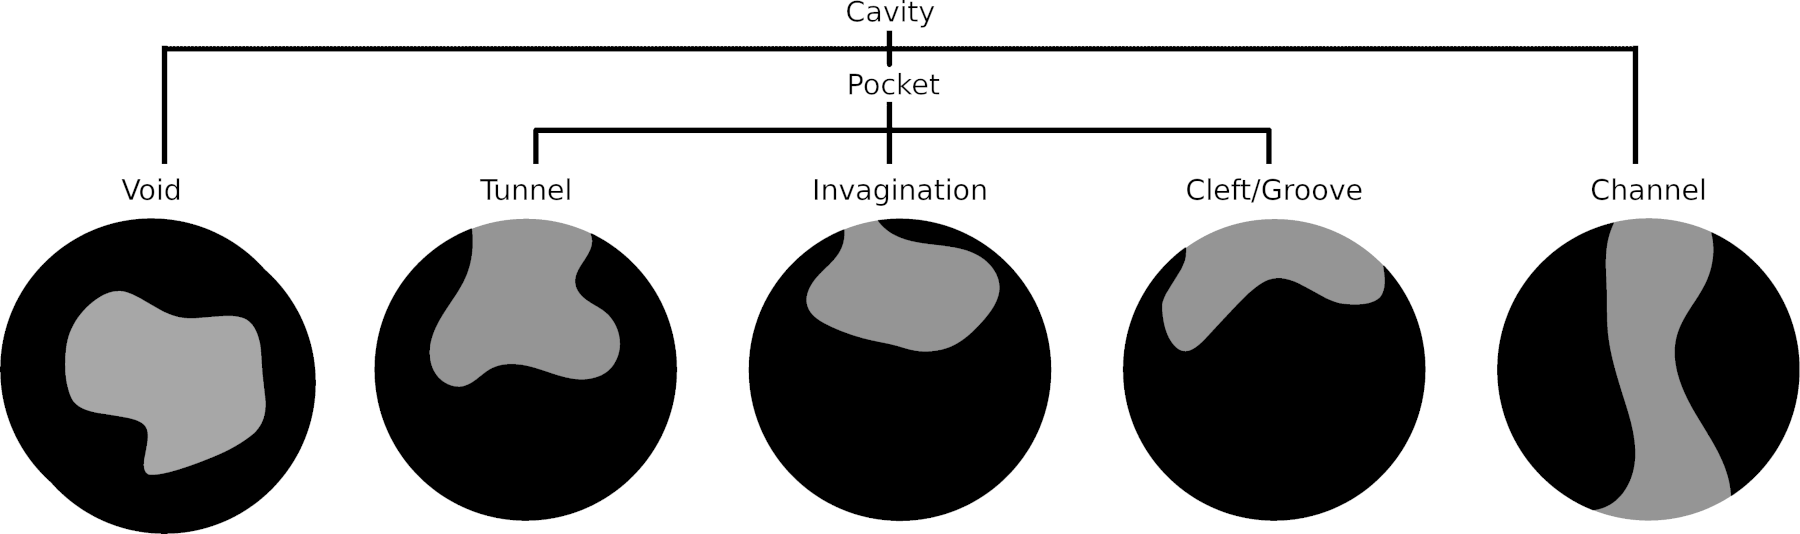
\includegraphics[scale=1]{images/cavity-classification.png}}
  \caption[Types of biomolecular cavities]{\textbf{Types of biomolecular cavities.} A biomolecular cavity (gray region) as a contiguous segment within the complement space of the biomolecule (black region), as defined by \cite{lay2013}. The categorization of these cavities follows an n-ary classification, where 'n' denotes the number of mouth openings. Specifically, a 0-ary cavity is identified as a void, representing an enclosed spatial configuration without external openings. In contrast, a 1-ary cavity, illustrated by a pocket, includes a single mouth opening. It is noteworthy that pockets encompass diverse forms like tunnels, invaginations, clefts, and grooves. Meanwhile, a 2-ary cavity, exemplified by a channel, features two mouth openings, facilitating the transit of molecular entities \cite{simoes2017}.}
  \label{fig:cavity-classification}
\end{figure}

In the current era of data science, the fields of computational and structural biology have significantly benefited from the increasing availability of biostructural data, as highlighted by \cite{mura2018}: "Structural biology meets data science". Advances in X-ray crystallography and electron microscopy techniques have expanded the determination of novel structures with respect to quality and size of these structures \cite{burley2018}. Biomolecules actively participate in various biological processes, such as protein folding, enzyme catalysis, DNA replication, DNA repair, cell signaling, virus-host interactions, and drug resistance. Dysregulation of these interactions is associated with numerous pathologies, including cancer, metabolic disorders, and pathogenic diseases \cite{scott2013}. For this reason, the identification and characterization of ligand-binding sites are the basis of rational structure-based drug discovery and design \cite{sotriffer2002,henrich2010}. Therefore, the imperative to identify targetable regions within the interaction area for new drugs becomes more apparent each day.

\section{Binding Site Characterization \label{sec:biomolecular-characterization}}

% The efficiency of identifying all cavities within a target protein using purely geometric approaches is noteworthy. However, the complexity arises in discriminating which of these cavities serve as functionally relevant binding sites \cite{sotriffer2002,henrich2010,liang1998,guerra2019}. While there is no simple and universally effective approach, characterizing binding sites based on their properties can lead to the identification of functionally relevant ones. As interactions within a cavity are inherently linked to its properties, elucidating these interactions becomes indispensable for determining the biological function of the biomolecule \cite{sotriffer2002,henrich2010}. 

Biomolecular interactions (\eg, \acs{PPI}, \acs{PLI}, \acs{PRI}, and \acs{PDI}) arise from distinctive property fingerprints at native or transient binding sites, where the molecular recognition hinges on the morphological, topological and physicochemical complementarity between the target biomolecule and its binding partner \cite{sotriffer2002,henrich2010,guerra2019,krone2016}. Binding sites impose morphological, topological and physicochemical constraints on putative ligands, with each interaction triggering a distinct biological function. Thus, describing potential binding sites in terms of morphological, topological, and physicochemical characteristics becomes essential for rational drug discovery and design, and assessing binding site druggability \cite{hubbard1994,liang1998,guerra2019,krone2016}.

The morphological attributes of biomolecular cavities establish stringent constraints on the geometry profiles of ligands capable of interacting efficiently within them. High affinity between the binding site and potential binders relies on sufficiently large interaction interfaces---extensive surface areas within the biomolecular cavity. The specificity of the binding site is dictated by geometric restrictions, including shape, size, and burial extent \cite{laskowski1996,liang1998}. Importantly, the cavity volume must accommodate the potential ligand \cite{stank2016}. The shape complementarity between the receptor and the ligand plays a decisive role in the binding process, with small ligands typically binding to buried concave sites on the molecular surface \cite{henrich2010}. Empirical studies have revealed that the active site often constitutes the largest and deepest cavity in enzymatic proteins \cite{laskowski1996}.

Topological characteristics of protein cavities contribute to functional analysis. The inference of the functionality of protein cavities has been achieved through comparison with homologous proteins, which exhibit homology and sequential similarity at the active site \cite{juncker2009}. Conserved local structural patterns, such as the catalytic triads of serine proteases \cite{dodson1998}, exemplify these homologous features. In enzymes, these specific configurations assume preferential spatial arrangements to execute elementary steps of the catalytic reaction, influencing the molecular recognition process of ligands by active sites \cite{sotriffer2002,henrich2010,thornton2000}. Describing a protein cavity according to the location of its different types of residues---hydrogen donors, electron receptors, hydrophobic contacts, and aromatics---becomes an insightful approach. Binding sites exhibit conserved amino acid sequences within protein families, offering valuable functional information \cite{henrich2010}. Amino acid composition distinguishes enzymatic from non-enzymatic binding sites, revealing varying compositions across different proteins \cite{guerra2019,carlson2008}.

Physicochemical characteristics play an essential role in selecting energetically favorable interactions. The synergy of van der Waals, hydrophobic, electrostatic, hydrogen bonding, and solvation interactions creates an energetically favorable environment for the binding process \cite{henrich2010}. For instance, hydrophobicity, quantified by the partition coefficient P, influences the kinetic and dynamic characteristics of drug action \cite{mannhold2009}. It is modulated by the shape of the binding site and the exposed area of residues \cite{henrich2010}. Various approaches generate distinct hydrophobicity scales for amino acids \cite{heiden1993}, such as Eisenberg \& Weiss \cite{eisenberg1984}, Hessa \& Heijne \cite{hessa2005}, Kyte \& Doolittle \cite{kyte1982}, Moon \& Fleming \cite{moon2011}, Radzicka \& Wolfenden \cite{radzicka1988}, Wimley \& White \cite{wimley1996}, and Zhao \& London \cite{zhao2006}. Conversely, the electrostatic potential, calculated by the Poisson-Boltzmann equation \cite{honig1995}, estimates ligand anchoring points, interaction free energy, biomolecule stability, and average atomic forces.

Therefore, the complexity lies in the discrimination which of these regions serve as functionally relevant binding sites, prompting the characterization of binding sites based on their distinctive properties \cite{sotriffer2002,henrich2010,liang1998,guerra2019}. Biomolecular interactions, shaped by morphological, topological, and physicochemical complementarity, form the foundation for understanding the biological function of biomolecules. While there is no simple and universally effective approach, characterizing binding sites based on their properties can lead to the identification of functionally relevant ones. As we unravel the intricate interplay of these properties, we gain essential insights into rational drug discovery, design, and the assessment of binding site druggability, marking a pivotal step toward advancing biomolecular research and therapeutic interventions \cite{sotriffer2002,henrich2010}.

\section{State of the Art \label{sec:state-of-the-art}}

Over the past decades, various \textit{in silico} have been developed for identifying binding sites in proteins to deepen our knowledge of a specific protein's function and for drug discovery and design \cite{liang1998}. However, only a few methodologies are applicable to other types of biomolecules, such as nucleic acids, carbohydrates, and lipids. The published computational approaches can be divided into three main categories: evolutionary, energetic, and geometric \cite{oliveira2014,simoes2017,guerra2019}.

\begin{itemize}
  \item \textbf{Evolutionary methods:} are based on the search for conserved residues in multiple sequence alignments and information from known binding site profiles;
  \item \textbf{Energetic methods:} identify binding sites based on the energetic interaction between the target biomolecule and a chemical probe, usually a chemical group;
  \item \textbf{Geometric methods:} identify cavities by analyzing the geometric characteristics of the molecular surface.
\end{itemize}

Each category of methods has its own advantages and disadvantages \cite{sotriffer2002,henrich2010,simoes2017}. Evolutionary algorithms heavily depend on sequence information or databases of active binding sites and the quality of the alignment procedure, while energetic methods rely on filtering procedures, force field parametrization, and applied scoring functions. On the other hand, geometric detection methods are relatively simple and straightforward, requiring no non-geometric knowledge, only structural data of the protein, \ie, the file in \ac{PDB}, XYZ, \ac{mmCIF}, or equivalent format, containing the Cartesian coordinates of atoms, easily accessible through the \ac{wwPDB}. Once atom coordinates are available, geometric methods should be able to represent any type of biomolecule \cite{henrich2010,oliveira2014,simoes2017}. Although purely geometric methods are efficient in identifying all types of cavities in a target molecule, identifying those that are functionally relevant poses a challenge. However, characterizing cavities in terms of well-chosen morphological, topological and physicochemical properties can lead to the identification of functionally relevant cavities, \ie, binding sites for a specific set of ligands \cite{sotriffer2002,henrich2010,liang1998,guerra2019}. 

In this context, geometry-based algorithms are the most widely used in the literature, as it is simple, direct, and does not require prior knowledge \cite{henrich2010,oliveira2014}. While evolution-based methods would be limited to proteins because they depend on principles of biological evolution, energy-based methods could be applicable but would require fine-tuning of force field parameters adapted to other types of biomolecules. As nucleic acids, carbohydrates, and lipids may have distinct properties compared to proteins, methods that rely solely on geometric information (e.g., \acs{3D} Cartesian coordinates and atom size) are desirable.

\subsection{Geometric Approaches \label{sec:geometric-approaches}}

The detection of cavities through geometric approaches is widespread, encompassing various techniques \cite{simoes2017,guerra2020}. These techniques are simple, straightforward, and do not require prior knowledge, making them the most commonly used in the literature \cite{henrich2010,oliveira2014}. In this context, we present a brief classification of geometric approaches for cavity detection (Figure \ref{fig:cavity-methods-infographic}), including techniques based on \ac{3D} grids, probes, surface, tessellation and their combinations \cite{simoes2017,guerra2020,guerra2023B}.

\begin{figure}[ht]
  \centering
  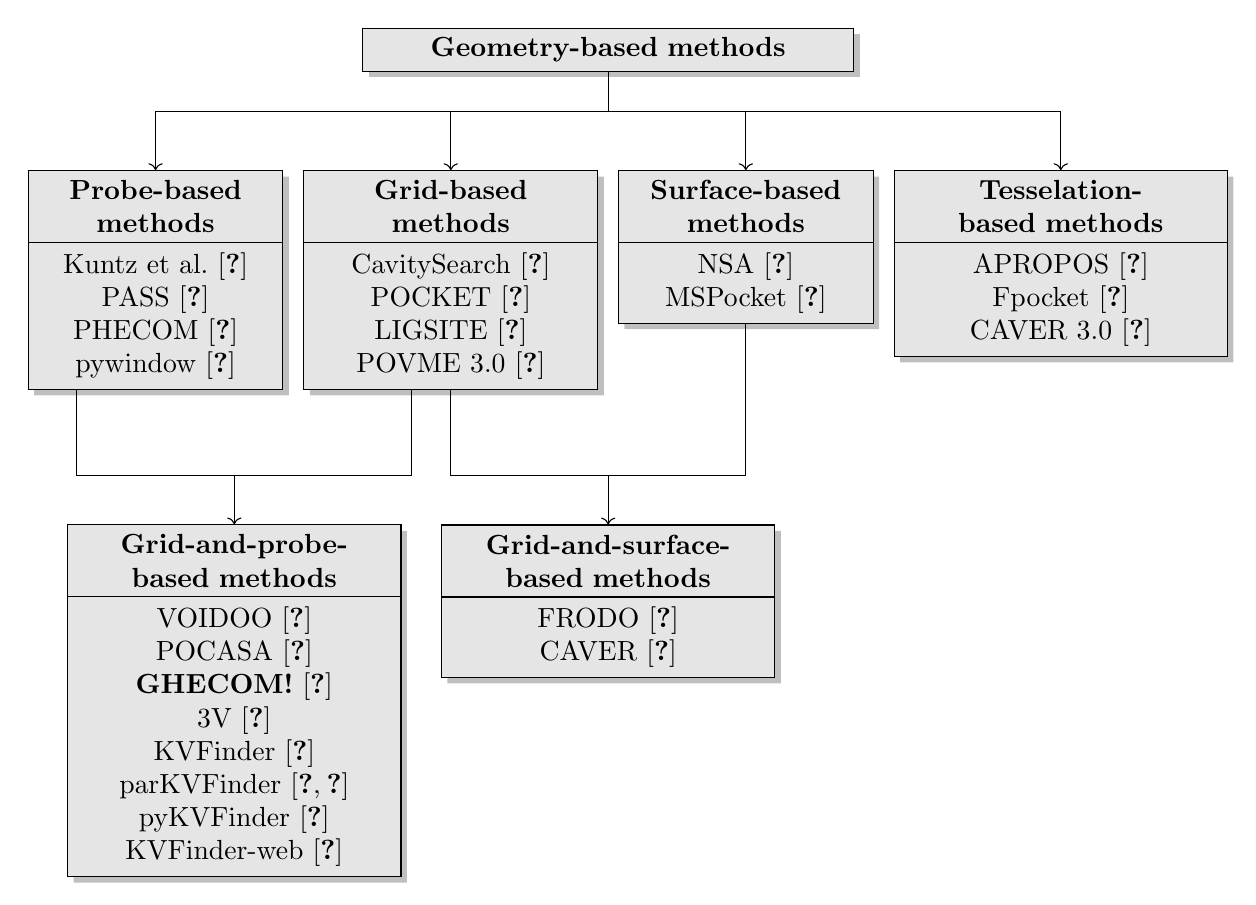
\begin{tikzpicture}[node distance=0.5cm]

    \node (GeomBased) [BoxNode, text width=6cm] {\textbf{Geometry-based methods}};
    \node (AuxNode01) [below=of GeomBased] {};
    \node (ProbeBased) [BoxNode, text width=3cm, rectangle split, rectangle split parts=2, below left=0.5cm and 4cm of AuxNode01] 
    {
      \textbf{Probe-based methods}
      \nodepart{two}{Kuntz et al. \ignorecitefornumbering{\cite{kuntz1982}}\\ PASS \ignorecitefornumbering{\cite{pass}}\\ PHECOM \ignorecitefornumbering{\cite{phecom}}\\ pywindow \ignorecitefornumbering{\cite{pywindow}}}
    };
    \node (GridBased) [BoxNode, text width=3.5cm, rectangle split, rectangle split parts=2, below left=0.5cm and 0cm of AuxNode01]
    {
      \textbf{Grid-based methods}
      \nodepart{two}{CavitySearch \ignorecitefornumbering{\cite{cavitysearch}}\\ POCKET \ignorecitefornumbering{\cite{pocket}}\\ LIGSITE \ignorecitefornumbering{\cite{ligsite}}\\ POVME 3.0 \ignorecitefornumbering{\cite{povme}}}
    };
    \node (SurfBased) [BoxNode, text width=3cm, rectangle split, rectangle split parts=2, below right=0.5cm and 0.0cm of AuxNode01]
    {
      \textbf{Surface-based methods}
      \nodepart{two}{NSA \ignorecitefornumbering{\cite{nsa}}\\ MSPocket \ignorecitefornumbering{\cite{mspocket}}}
    };
    \node (TessBased) [BoxNode, text width=4cm, rectangle split, rectangle split parts=2, below right=0.5cm and 3.5cm of AuxNode01]
    {
      \textbf{Tesselation-based methods}
      \nodepart{two}{APROPOS \ignorecitefornumbering{\cite{apropos}}\\ Fpocket \ignorecitefornumbering{\cite{fpocket}}\\ CAVER 3.0 \ignorecitefornumbering{\cite{caver3}}}
    };
    \node (AuxNode02) [below left=4.25cm and 4.7cm of AuxNode01] {};
    \node (AuxNode03) [below left=4.25cm and 4.3cm of AuxNode01] {};
    \node (AuxNode04) [below left=4.25cm and 4.5cm of AuxNode01] {};
    \node (GPBased) [BoxNode, rectangle split, rectangle split parts=2, below=0.5cm of AuxNode04, text width=4cm]
    {
      \textbf{Grid-and-probe-based methods}
      \nodepart{two}{VOIDOO \ignorecitefornumbering{\cite{voidoo}}\\ POCASA \ignorecitefornumbering{\cite{pocasa}}\\ \acs{GHECOM} \ignorecitefornumbering{\cite{ghecom}}\\ 3V \ignorecitefornumbering{\cite{3v}}\\ KVFinder \ignorecitefornumbering{\cite{oliveira2014}}\\ parKVFinder \ignorecitefornumbering{\cite{guerra2019,guerra2020}}\\ pyKVFinder \ignorecitefornumbering{\cite{guerra2021}}\\ KVFinder-web \ignorecitefornumbering{\cite{guerra2023A}}}
    };
    \node (GSBased) [BoxNode, rectangle split, rectangle split parts=2, below=5cm of AuxNode01, text width=4cm]
    {
      \textbf{Grid-and-surface-based methods}
      \nodepart{two}{FRODO \ignorecitefornumbering{\cite{frodo}}\\ CAVER \ignorecitefornumbering{\cite{caver}}}
    };
    \node (AuxNode05) [below left=4.25cm and 0.0cm of AuxNode01] {};
    \node (AuxNode06) [below right=4.25cm and 0.0cm of AuxNode01] {};
    \node (AuxNode07) [below=4.25cm of AuxNode01] {};

    \draw [->] (GeomBased.south) -- (AuxNode01)+(0,0.12) -| (ProbeBased.north);
    \draw [->] (GeomBased.south) -- (AuxNode01)+(0,0.12) -| (GridBased.north);
    \draw [->] (GeomBased.south) -- (AuxNode01)+(0,0.12) -| (SurfBased.north);
    \draw [->] (GeomBased.south) -- (AuxNode01)+(0,0.12) -| (TessBased.north);
    \draw [-] (ProbeBased.south)+(-1,0) |- (AuxNode03);
    \draw [->] (GridBased.south)+(-0.5,0) |- (AuxNode02)-| (GPBased.north);
    \draw [-] (SurfBased.south)+(0,0) |- (AuxNode05);
    \draw [->] (GridBased.south)+(0,0) |- (AuxNode06)-| (GSBased.north);

  \end{tikzpicture}
  \caption[Classification of geometry-based methods]{\textbf{Classification of geometry-based methods.}}
  \label{fig:cavity-methods-infographic}
\end{figure}

\begin{itemize}
  \item \textbf{Grid-based algorithms} (\eg, CavitySearch \cite{cavitysearch}, POCKET \cite{pocket}, LIGSITE \cite{ligsite}, POVME 3.0 \cite{povme}) represent a set of atoms as discrete points, usually using a \acs{3D} grid aligned to the axes as a scalar field, \ie, a density map, where each discrete point is an integer or boolean value. These grid maps are used to cluster relevant empty space points (\ie, not belonging to the solute) into cavities using voxel clustering algorithms. Typically, these methods use simple data structures capable of representing a collection of data at a discrete point and identifying cavities automatically. However, geometric accuracy, computation time, and memory consumption heavily depend on the grid resolution, \ie, grid-spacing sensitivity. Additionally, these methods are not rotationally invariant, meaning that the orientation of a given molecule slightly affects accuracy, \ie, orientation sensitivity;
  \item \textbf{Probe-based algorithms} (\eg, Kuntz et al. \cite{kuntz1982}, PASS \cite{pass}, PHECOM \cite{phecom}, pywindow \cite{pywindow}) use a set of atoms, considering their \acs{3D} coordinates and \ac{vdW} radii, to represent the molecular surface, which is analyzed by one or more probes, usually rigid spheres, to investigate its accessibility levels. This technique can detect any type of cavity and is related to the spatial extension of potential ligands; however, it may struggle to find and unequivocally delineate the boundaries between the cavity and the solvent, \ie, mouth-opening ambiguity;
  \item \textbf{Surface-based algorithms} (\eg, NSA \cite{nsa}, MSPocket \cite{mspocket}) do not use a rigid sphere model but rather a molecular surface model, such as \acs{vdW} surface, \ac{SES}, \ac{SAS}, and \ac{LES}, defining the molecular interface and its environment. Analysis of the molecular interface identifies cavities based on accessibility to a specific solvent or ligand. In this case, cavity detection occurs automatically, as in grid-based methods, but without mouth-opening ambiguity. However, in some cases, these algorithms may struggle to detect all types of cavities and their complete extent;
  \item \textbf{Tessellation-based algorithms} (\eg, APROPOS \cite{apropos}, Fpocket \cite{fpocket}, CAVER 3.0 \cite{caver3}) rely on computational geometry techniques, such as \textalpha-shapes, \textbeta-shapes, Voronoi diagrams, and Apollonius diagrams. Specifically, \textalpha-shapes and Voronoi tessellation use atomic centers, implicitly constant-radius spheres to model atoms, while \textbeta-shapes and Apollonius-based methods depend on variable-radius spheres to model these atoms, which are explored to identify cavities. Typically, these methods do not depend on any information from the molecular surface to detect cavities but may struggle to identify the correct binding site location, delineate the boundaries between the cavity and the solvent, and define the number of surface atoms.
\end{itemize}

This classification illustrates that each technique has its own inherent strengths and weaknesses, rendering them more suitable for specific applications \cite{simoes2017,guerra2020}. The cohesive combination of these techniques aims to leverage the capabilities of each and mitigate their individual shortcomings, resulting in more robust approaches. Within this broader context, two notable subcategories emerge:

\begin{itemize}
  \item \textbf{Grid-and-probe-based methods} (\eg, VOIDOO \cite{voidoo}, POCASA \cite{pocasa}, \acs{GHECOM} \cite{ghecom}, 3V \cite{3v}, KVFinder \cite{oliveira2014}, parKVFinder \cite{guerra2019,guerra2020}) combine the strengths of both grid- and probe-based methods. Analogous to grid-based methods, they rely on a scalar field defined at each grid point and predominantly use large probe spheres rolling on the \acs{vdW} surface. These probes define cavities between the probe-generated surface and the molecular surface. This combined approach mitigates mouth-opening ambiguity and orientation sensitivity, common in grid-based methods \cite{simoes2017}. The mouth-opening ambiguity is also known as cavity ceiling problem, which can be controlled by customizable probe sizes \cite{simoes2017,oliveira2014}. However, grid-spacing sensitivity remains, unless we use a grid spacing of at most half of the smaller probe to mitigate it. The usage of probes in grid-based methods follows three techniques, that are atom fattening (originating \acs{SAS} or \acs{SAS}-like surfaces), exemplified by VOIDOO \cite{voidoo}, rolling probes of unequal radii on the \acs{vdW} surface, as seen in POCASA \cite{pocasa}, \acs{GHECOM} \cite{ghecom}, and 3V \cite{3v}, and concentric probes of unequal radii at grid points, specifically implemented in KVFinder software \cite{oliveira2014};
  \item \textbf{Grid-and-surface-based methods} (\eg, FRODO \cite{frodo}, CAVER \cite{caver}) combine the strengths of both grid- and surface-based methods. Similar to probe spheres, surfaces resolve the ambiguity issue in grid-based methods, particularly in defining cavity ceilings (and, consequently, mouth openings). These methods employ a scalar field in conjunction with a \acs{3D} grid, where the scalar field may be defined by various functions. In summary, the utilization of surfaces with grids overcomes common issues associated with grid-based methods, namely, orientation sensitivity and mouth-opening ambiguity. However, the challenge of grid-spacing sensitivity persists unless a grid spacing of at most half of the smaller probe.
\end{itemize}

In this context, the exploration of geometric approaches for cavity detection reveals a diverse landscape of techniques, each with its unique strengths and weaknesses. The simplicity and accessibility of these methods have made them foundational in biomolecular research \cite{henrich2010,simoes2017}. This classification, encompassing grid-based, probe-based, surface-based, and tessellation-based algorithms, provides a comprehensive overview of the strategies employed in structural and functional characterization of biomolecules and binding sites \cite{simoes2017}. The cohesive integration of these techniques, as seen in grid-and-probe-based or grid-and-surface-based methods, represents a strategic effort to overcome individual limitations and enhance the robustness of cavity detection methodologies. By acknowledging the strengths of each approach and strategically combining them, researchers aim to optimize the efficacy of computational platforms, paving the way for more nuanced and accurate structural and functional insights into biomolecules.

\subsection{Well-established Computational Tools \label{sec:computational-tools}}

The vast majority of cavity detection tools were originally developed for proteins (see Section \ref{sec:geometric-approaches}). Although these algorithms exhibit robustness in describing and analyzing any molecular system (\eg, protein, DNA, RNA, inorganic material, supramolecular cage, etc.), so far, only a few tools have been applied to other biomolecular systems, excluding proteins, to assess structural characteristics such as the shape, volume, area and mouth openings. Our literature review led us to identify tools meeting specific criteria: applicability to any molecular system, availability as free software, comprehensive documentation, robust developer support, a well-conceived set of characterizations, and recognition within the scientific community. Guided by these stringent criteria, we spotlight four well-established cavity detection tools: parKVFinder, Fpocket, \acs{GHECOM}, and CAVER tools.

\subsubsection{parKVFinder}

parKVFinder \cite{guerra2019,guerra2020}, a grid-and-probe-based approach, detects and characterizes any type of biomolecular cavity, integrated with a graphical plugin for PyMOL \cite{pymol}. The cavity detection algorithm (Figure \ref{fig:parkvfinder-schema}) employs a dual-probe methodology based on mathematical morphology theory \cite{matheron1974,serra1982}. Originally implemented in the KVFinder software \cite{oliveira2014}, this algorithm involves two probes, a smaller probe (\textit{Probe In}) and a larger probe (\textit{Probe Out}), inspecting grid points to define cavities as the non-overlapping regions traversed by these probes.

\begin{figure}[h]
  \centerline{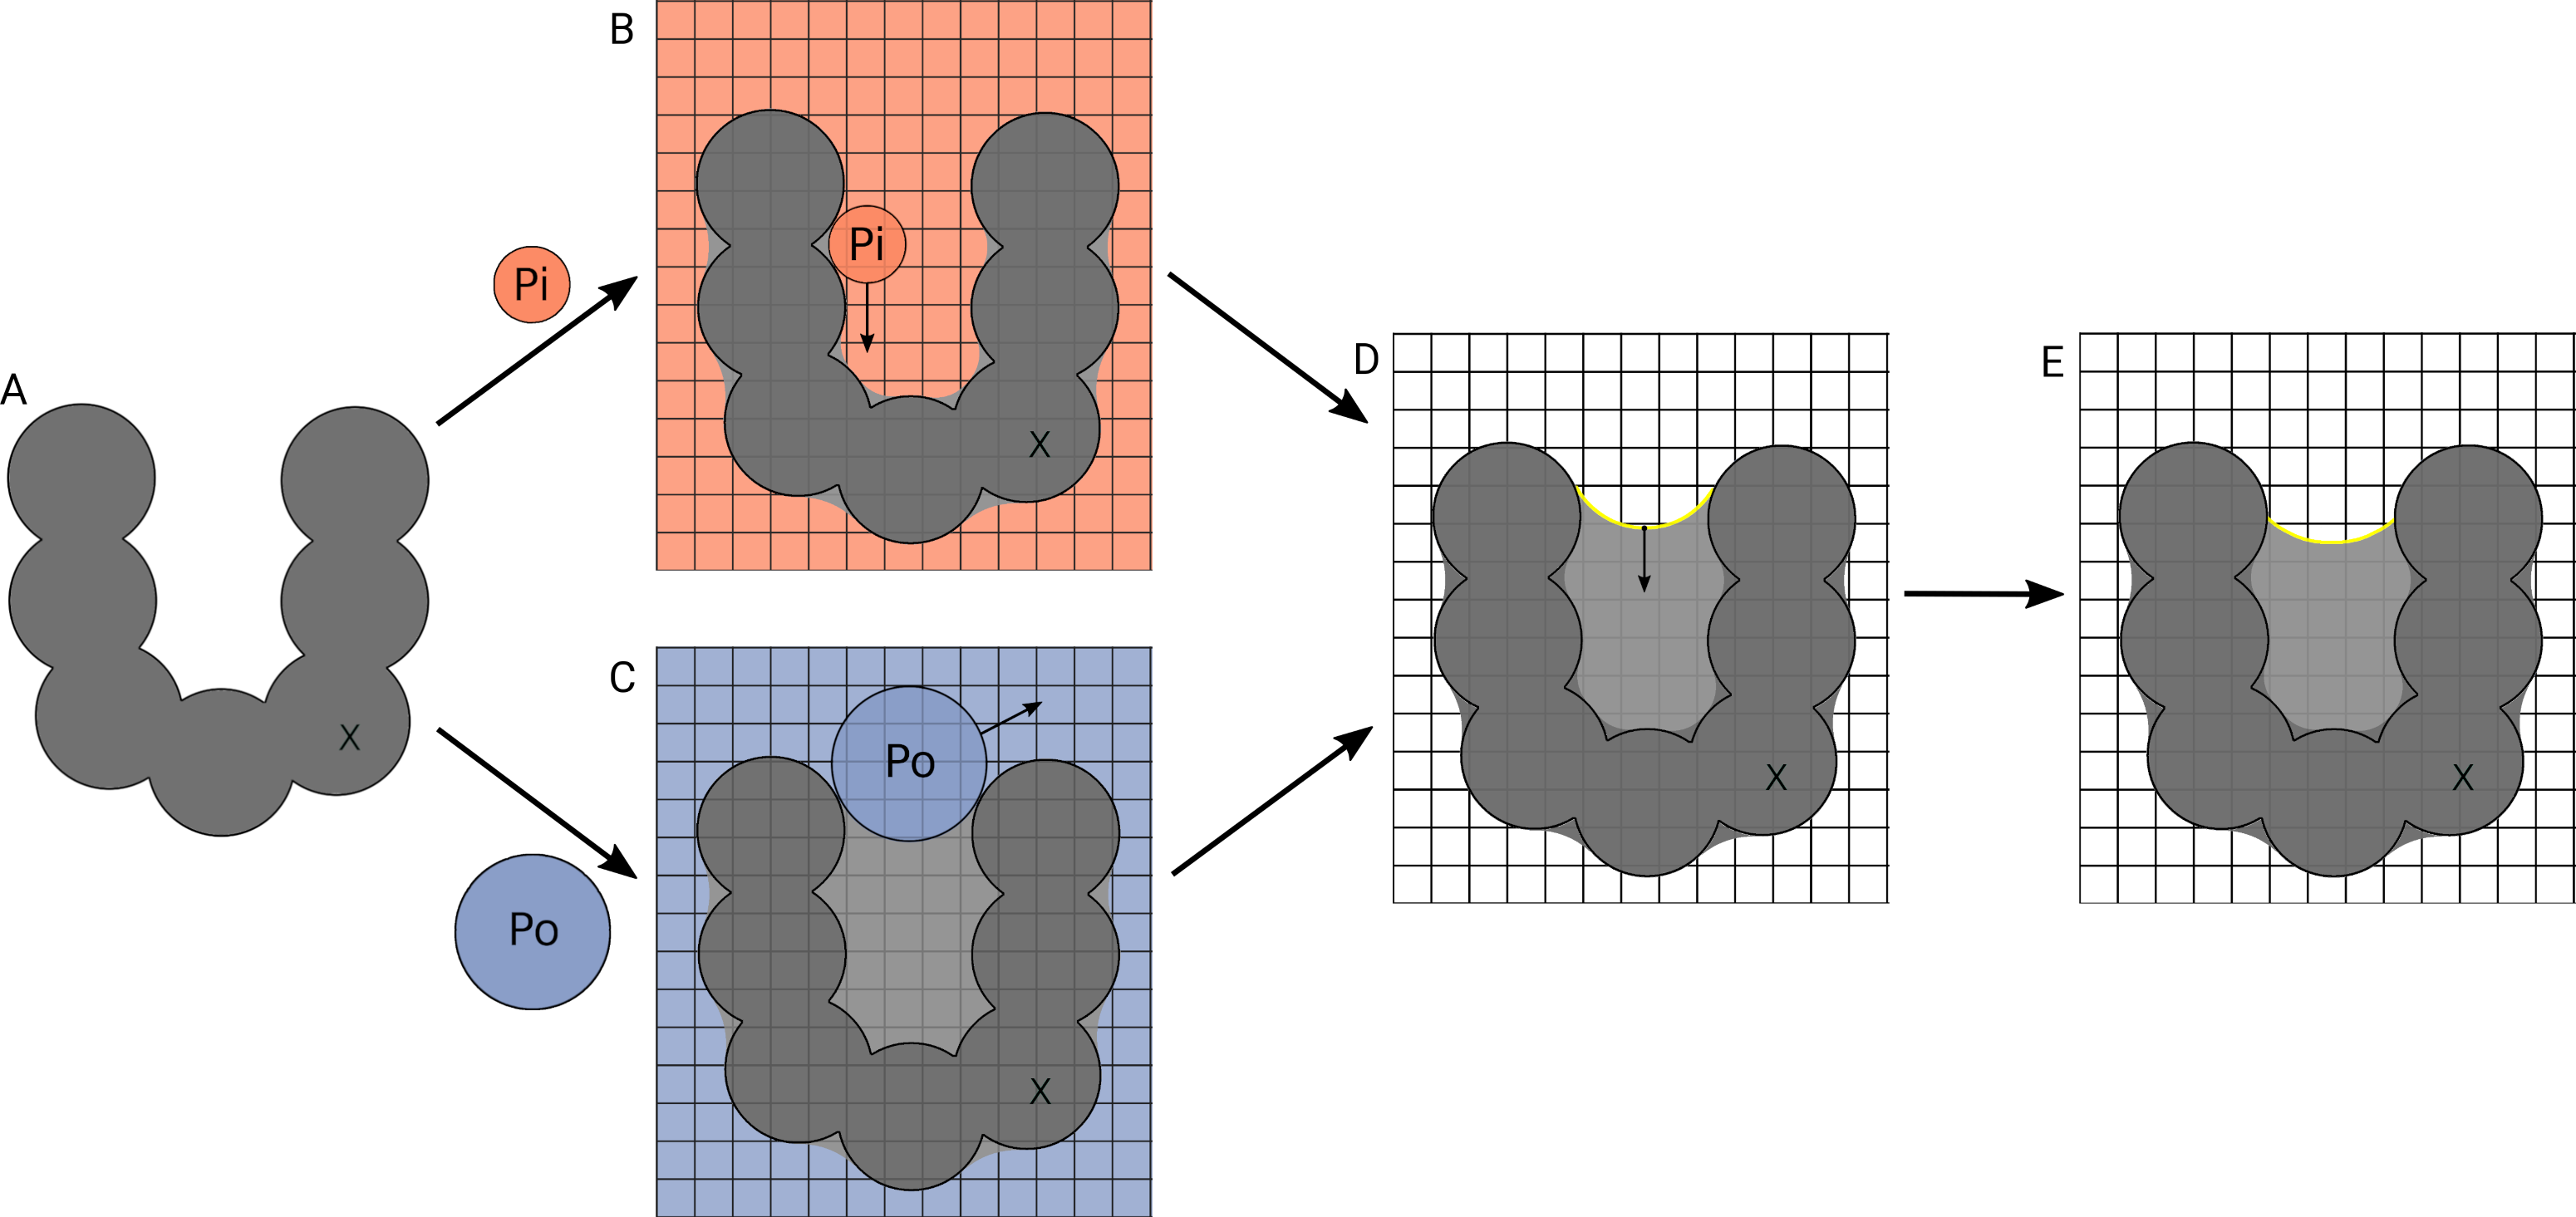
\includegraphics[scale=1]{images/kvfinder-suite-schema.png}}
  \centerline{\tiny{\textbf{Source:} Reprinted with permission from \cite{guerra2023B}. Copyright 2023 American Chemical Society.}}
  \caption[Cavity detection algorithm in parKVFinder]{\textbf{Cavity detection algorithm in parKVFinder.} \textbf{(A)} A biomolecular structure X, composed of atoms modeled as rigid spheres with van der Waals radii, is inserted into a \acs{3D} grid. \textbf{(B)} The \ac{Pi} probe traverses the surface of the structure, moving through grid points (orange). \textbf{(C)} Next, the \ac{Po} probe traverses accessible points in blue. \textbf{(D)} Cavity points (light gray) are defined as the difference between the accessible points of the probes. Points not reached by \acs{Pi} (dark gray) define the \acs{SES} (standard) or \acs{SAS}, depending on the surface representation chosen by the user. \textbf{(E)} Finally, a distance-based removal procedure is applied to eliminate cavity points near the cavity-bulk boundary (yellow line).}
  \label{fig:parkvfinder-schema}
\end{figure}

It is noteworthy that the original KVFinder software \cite{oliveira2014}, introduced in 2014, has been deprecated. However, subsequent implementations, namely parKVFinder \cite{guerra2020}, pyKVFinder \cite{guerra2021}, and KVFinder-web \cite{guerra2023A}, have been developed to enhance computational performance and usability. Each of these tools addresses different scientific community demands in a flexible manner. Cavity characterization in these tools includes morphological descriptors (\eg, volume, area, shape, and depth), topological descriptors (\eg, interface residues surrounding the cavities and their classification---aliphatic, aromatic, polar uncharged, negatively charged, and positively charged---), and physicochemical descriptors (\eg, hydrophobicity). Further details on the parKVFinder can be found in Section \ref{sec:parkvfinder}.

\subsubsection{Fpocket}

Fpocket \cite{fpocket}, a tessellation-based approach, employs the concept of \textalpha\space spheres, originally introduced by \cite{liang1998}, for the detection of molecular pockets. The cavity detection algorithm (Figure \ref{fig:fpocket-schema}) performs a comprehensive analysis to identify the whole set of \textalpha\space spheres within a given molecular structure, using the \textit{qhull} package \cite{qhull}. The process involves categorizing small alpha spheres situated inside the structure, large spheres outside the structure, and the spheres in between as corresponding to cavities. To refine the cavity selection, Fpocket eliminates any alpha sphere falling outside a customized range of minimum and maximum radii. The remaining \textalpha\space spheres are grouped into cavities based on proximity and neighborhood relationships, and cavities of poor interest (\eg, hydrophilic or small putative pockets) excluded from further analysis. Subsequently, the cavities are assessed using a set of dpocket descriptors \cite{fpocket}, allowing the cavities to be ranked according to their putative binding affinity for small molecules. 

\begin{figure}[ht]
  \centerline{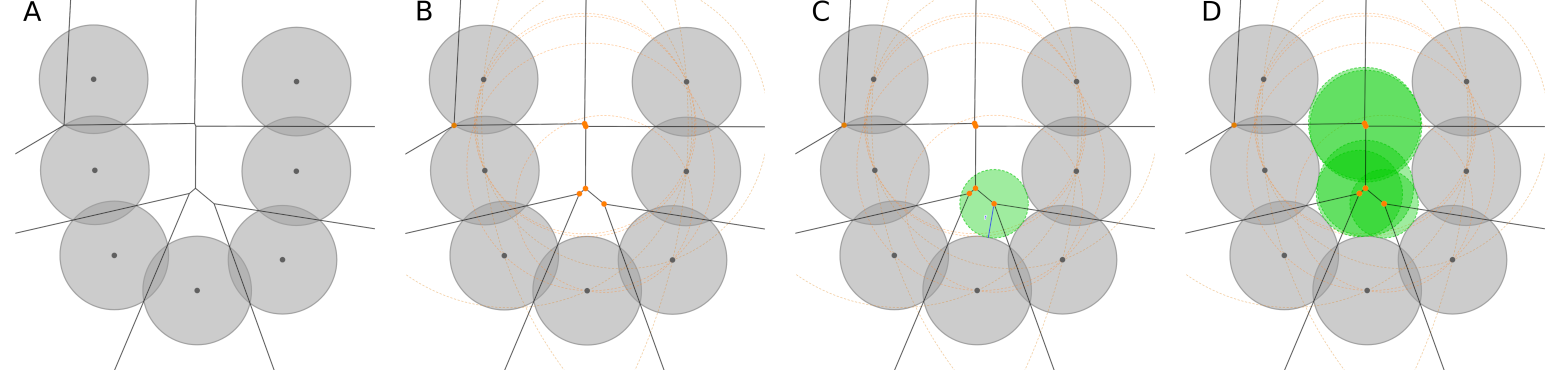
\includegraphics[scale=0.9]{images/fpocket-schema.png}}
  \centerline{\tiny{\textbf{Source:} Reprinted with permission from \cite{guerra2023B}. Copyright 2023 American Chemical Society.}}
  \caption[Cavity detection algorithm in Fpocket]{\textbf{Cavity detection algorithm in Fpocket.} \textbf{(A)} Voronoi diagram of the atomic centers. \textbf{(B)} Voronoi balls (dotted orange circles) centered at Voronoi vertices (orange points). \textbf{(C)} Example of an \textalpha\space sphere (green sphere) centered at a Voronoi vertex (orange point) and grows until it becomes tangent to an atom. \textbf{(D)} Cluster of \textalpha\space spheres (green region) filling the binding site.}
  \label{fig:fpocket-schema}
\end{figure}

\subsubsection{\acs{GHECOM}}

\ac{GHECOM} \cite{ghecom}, a grid-and-probe-based approach, identifies both deep and shallow pockets, employing an array of spherical probes. The cavity detection algorithm (Figure \ref{fig:ghecom-schema}) combines fundamental erosion and dilation operations from mathematical morphology \cite{matheron1974,serra1982} with different spherical probes to report openness-closedness of a target molecular shape, thereby revealing deep and shallow pockets (referred to as \textit{multi-scale pockets}). Following that, a single-linkage clustering method groups pocket regions, allowing for the subsequent estimation of their respective volumes. \acs{GHECOM} introduces a metric known as \textit{pocketness}, which establishes a correlation between the volume and depth of points associated with individual residues or atoms. This metric serves as an informative indicator of their respective contributions to ligand interactions.

\begin{figure}[H]
  \centerline{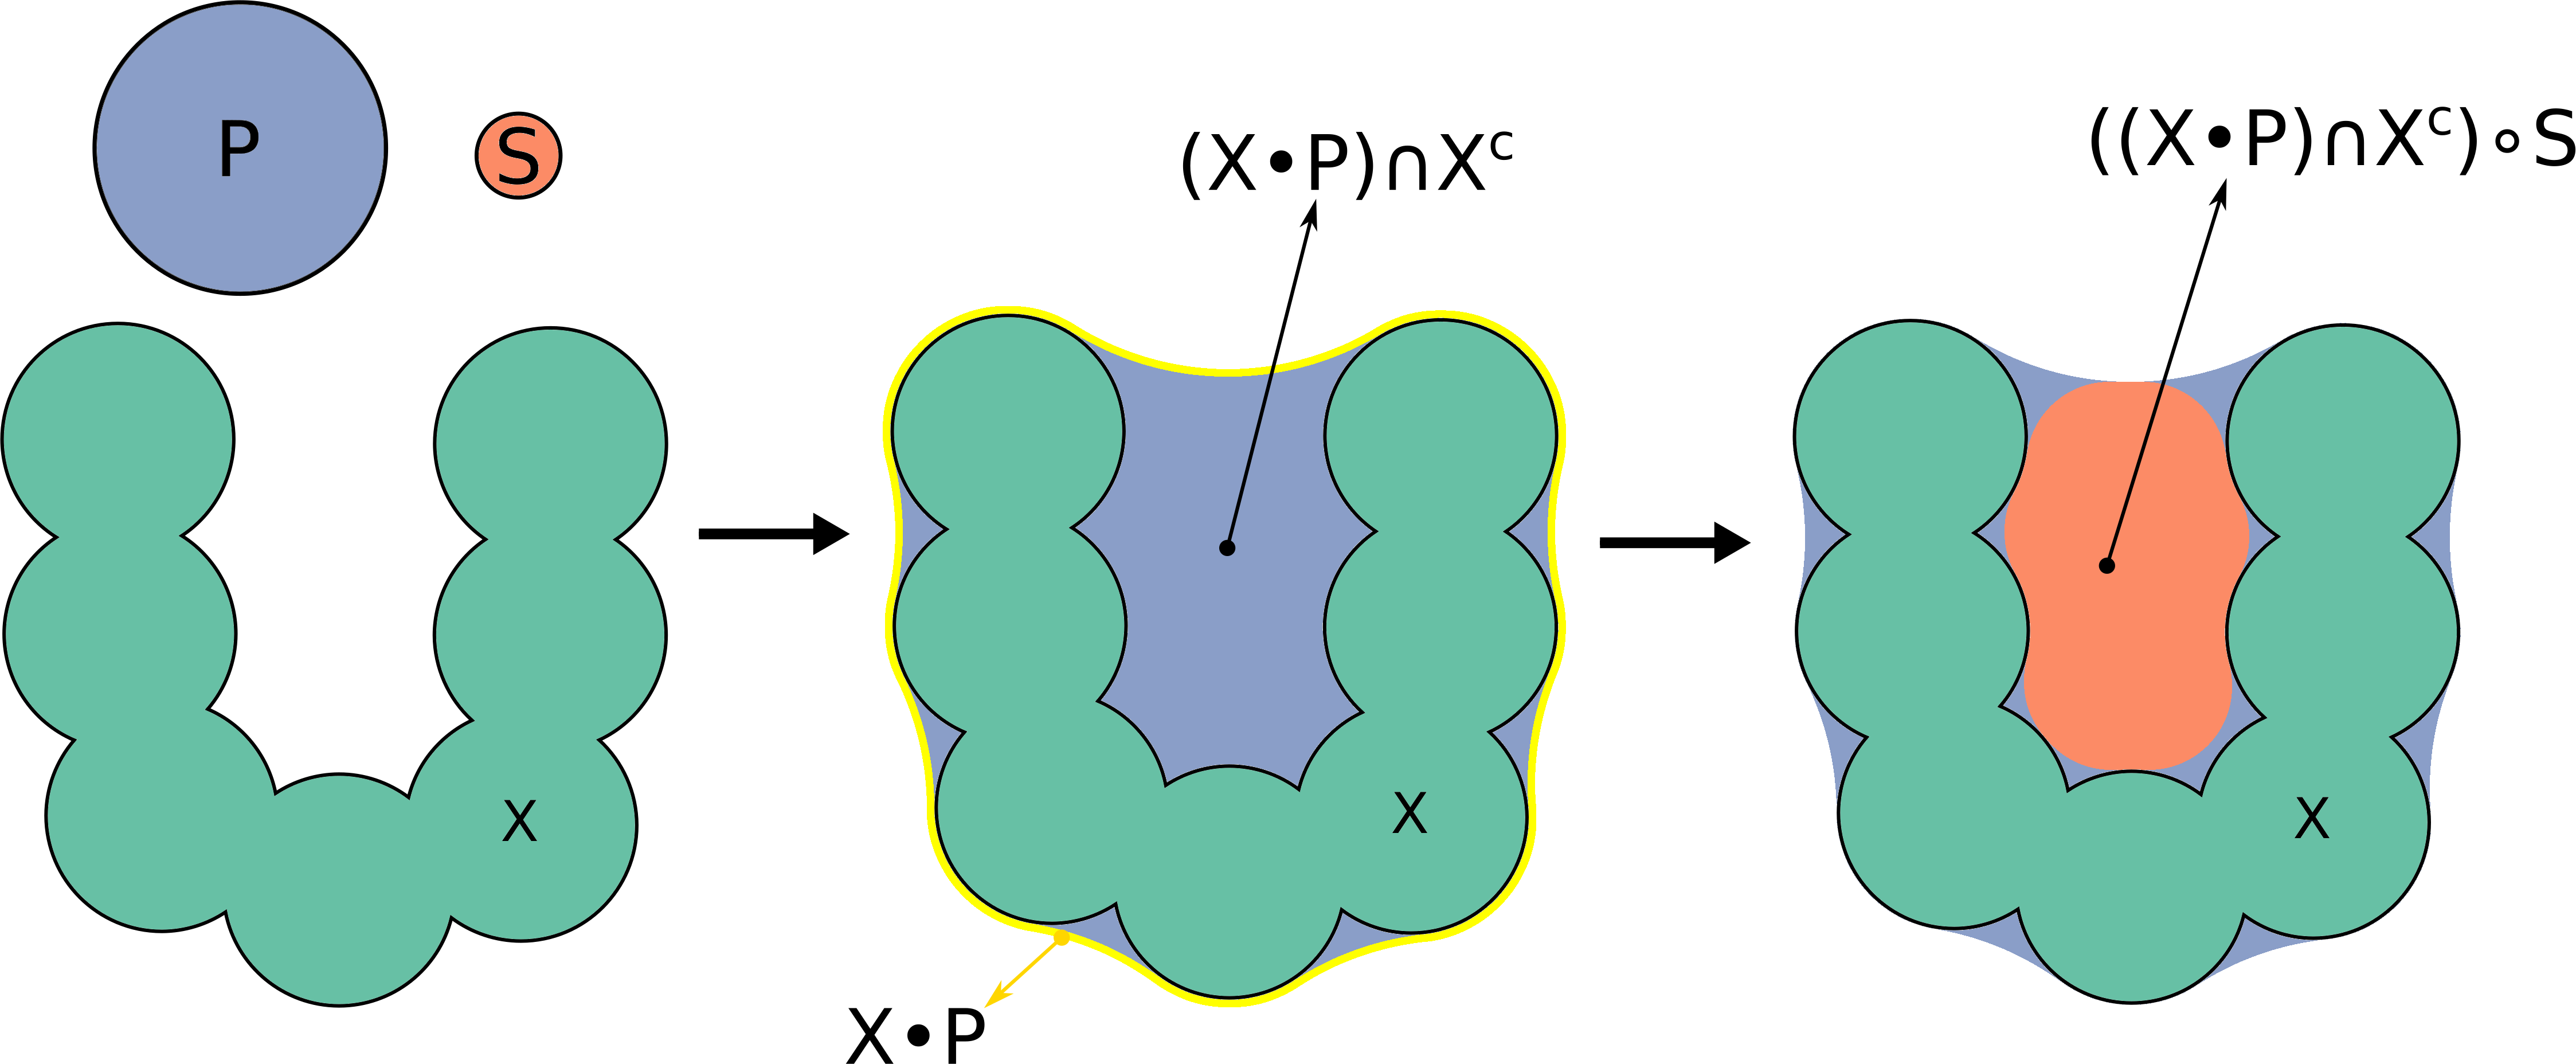
\includegraphics[scale=0.9]{images/ghecom-schema.png}}
  \centerline{\tiny{\textbf{Source:} Reprinted with permission from \cite{guerra2023B}. Copyright 2023 American Chemical Society.}}
  \caption[Pocket detection algorithm in \acs{GHECOM}]{\textbf{Pocket detection algorithm in \acs{GHECOM}.} A biomolecular structure (green region; $X$) is enclosed by a spherical probe P (blue sphere), defining the region bounded by the yellow contour. Next, the intersection of X closed by P ($X \bullet P$) and the space outside the protein ($X^c$) defines the region not accessible to the probe P (blue region; $(X \bullet P) \cap X^c$). Subsequently, this region is opened by a spherical probe S (orange sphere), where P is larger than S. Finally, the pocket (orange region; $((X \bullet P) \cap X^c) \circ S$) is defined by the space outside the molecular shape not accessible to P but accessible to S. For multi-scale detection, different sizes of the spherical probe P are used.}
  \label{fig:ghecom-schema}
\end{figure}

\subsubsection{CAVER tools}

CAVER tools comprise a series of computational methods designed for tunnel and channel analysis within biomolecular structures. The initial iteration, CAVER \cite{caver}, was a grid-and-surface-based approach for tunnel and channel calculation. Subsequently, CAVER 3.0 \cite{caver3} replaced the axis-aligned grid with a Voronoi diagram approach, turning into a tessellation-based approach. The user-friendly interface, CAVER Analyst 2.0 \cite{caveranalyst2}, incorporates CAVER 3.0, providing visual assistance to users in tunnel and cavity calculations. The cavity detection algorithm (Figure \ref{fig:caver-schema}) constructs a pseudo-Voronoi diagram of a given biomolecular structure. By identifying paths represented as graphs composed of Voronoi vertices and edges, CAVER 3.0 characterizes these paths as tunnels connecting cavities to the surrounding solvent. The resulting tunnels are further characterized by length, average radius, and bottleneck (mouth opening) radius. CAVER Analyst 2.0 complements these functionalities by identifying regions of empty space (\ie, cavities) within the biomolecular structure. Employing a similar approach to that described in the KVFinder suite (Figure \ref{fig:parkvfinder-schema}) and \acs{GHECOM} (Figure \ref{fig:ghecom-schema}), CAVER Analyst 2.0 determines regions accessible where a small probe can enter from outside, but a large probe cannot.

\begin{figure}[H]
  \centerline{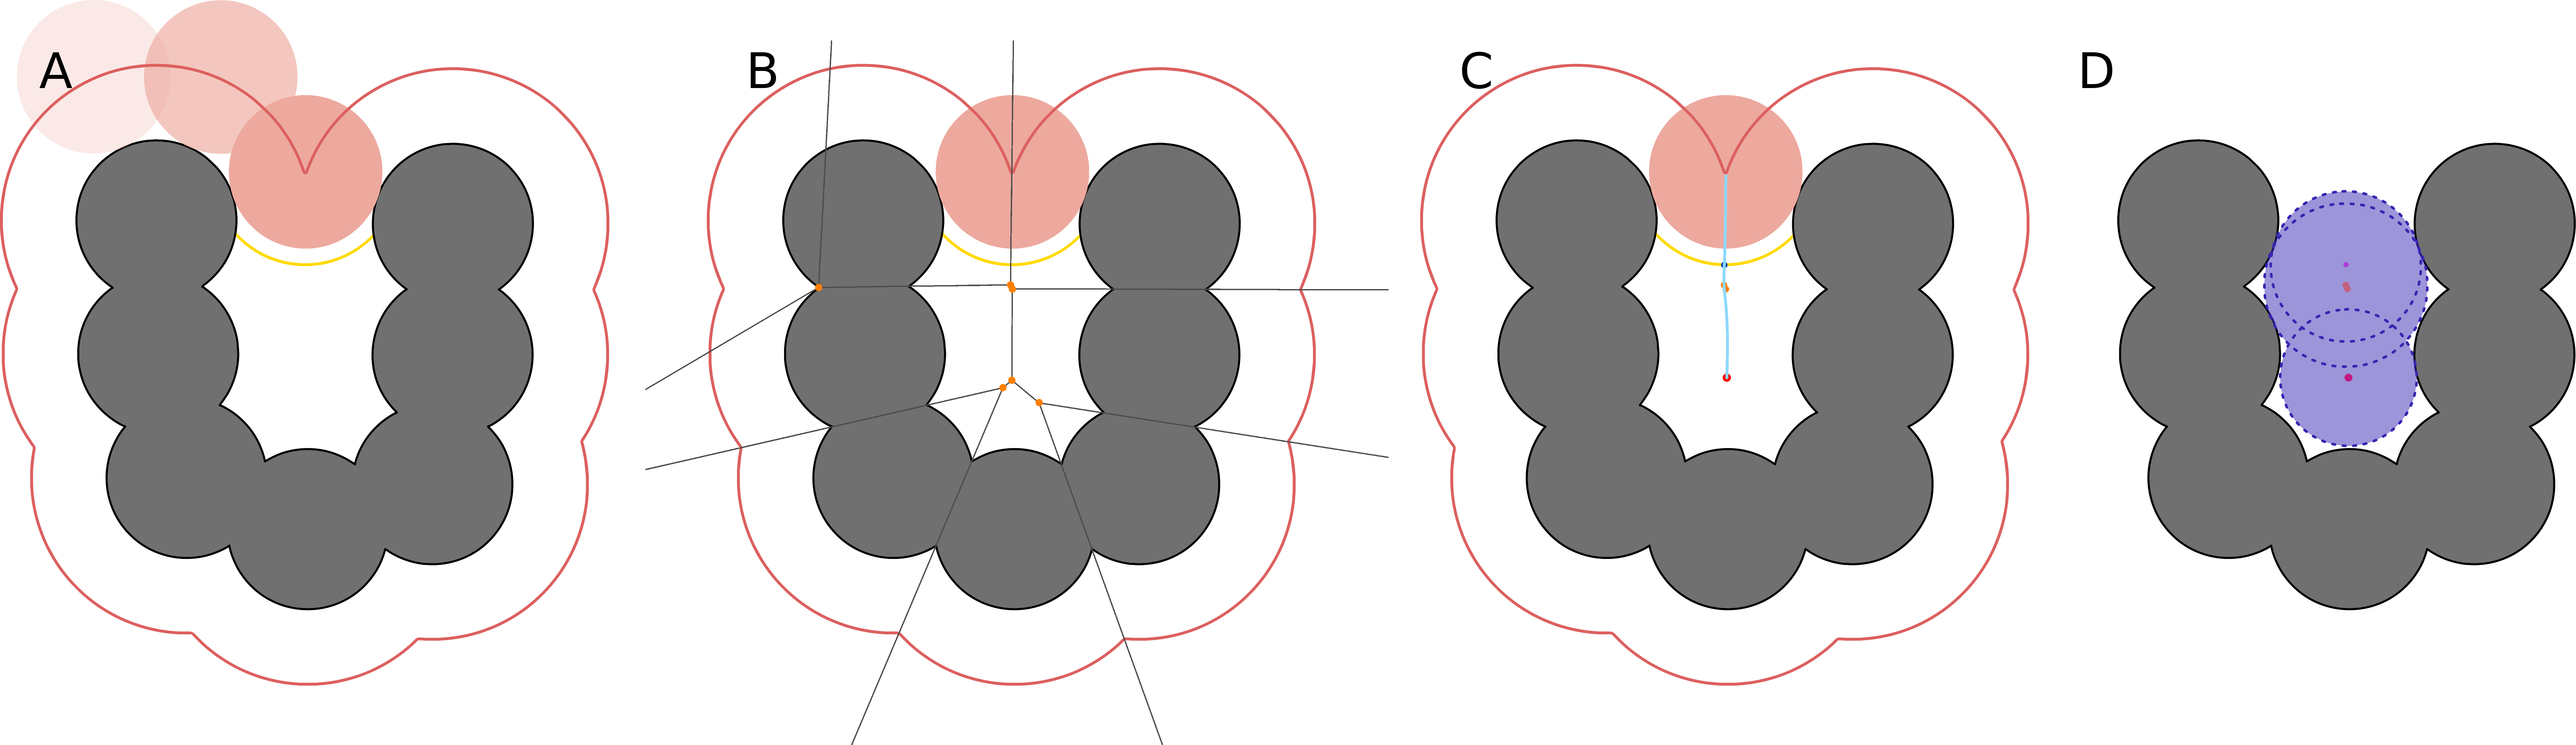
\includegraphics[scale=1.1]{images/caver-schema.png}}
  \centerline{\tiny{\textbf{Source:} Reprinted with permission from \cite{guerra2023B}. Copyright 2023 American Chemical Society.}}
  \caption[Channel and tunnel detection algorithm in CAVER 3.0]{\textbf{Channel and tunnel detection algorithm in CAVER 3.0.} \textbf{(A)} A molecular shape is probed by a spherical probe, called the \textit{shell probe}, with a radius specified by the \textit{shell radius} parameter, to define an outer surface \acs{SAS} (red line). From it, a distance specified by the \textit{shell depth} parameter is removed to define an inner surface (yellow line). \textbf{(B)} A pseudo-Voronoi diagram is constructed based on the molecular shape. Voronoi vertices (orange points) are used to create the central lines of the tunnel/channel. \textbf{(C)} A starting point (red point) is a user-defined parameter set as the center of mass of the molecular shape, and an endpoint (blue point) is set at the center of the inner surface. From the starting point, the central line passes through Voronoi edges and vertices to form a tunnel/channel to the outer surface and passes through the endpoint. \textbf{(D)} Spheres are fitted at all points of the central line, from the starting point to the endpoint, defining the bottleneck (mouth opening) radius along the tunnel and/or channel.}
  \label{fig:caver-schema}
\end{figure}

\section{Computational Complexity \label{sec:computational-complexity}}

The effectiveness of cavity detection algorithms relies not only on their accuracy in identifying binding sites but also on their computational efficiency, particularly when dealing with biomolecular structures and large datasets. Computational complexity, a field studying algorithmic efficiency, involves analyzing the computational resources, such as time and space, required by an algorithm to solve a specific problem as a function of the input size. The goal is to understand how an algorithm's performance scales with increasing input sizes.

There are two primary aspects of computational complexity:

\begin{itemize}
  \item \textbf{Time Complexity:} measures the time an algorithm takes to complete relative to the input size;
  \item \textbf{Space Complexity:} measures the memory (\ie, space) an algorithm needs to solve a problem based on the input size.
\end{itemize}

In computer science, both time and space complexity are often expressed using big-O notation ($\mathcal{O}$), also known as Bachmann-Landau notation. This notation describes the upper bound of an algorithm's running time and memory requirements, respectively, classifying algorithms based on how their performance grows relative to the input size.

In this scenario, the computational complexity of cavity detection algorithms is a
critical aspect that influences their practical utility and scalability. Here, we briefly delve into the computational complexity of the geometry-based approaches described in Section \ref{sec:geometric-approaches}.

Grid-based algorithms (\eg, CavitySearch \cite{cavitysearch}, POVME 3.0 \cite{povme}) rely on discretizing the molecular structure into a \acs{3D} grid. The computational complexity of these methods is inherently tied to the grid spacing and biomolecule size. The time complexity is typically $\mathcal{O}(n_{v})$, where $n_{v}$ represents the number of voxels, and it linearly increases with the number of voxels. In terms of user inputs, the number of voxels (Eq. \ref{eq:nv-ref}) is expressed as follows:

\begin{equation}
  n_v \colon (l_x,l_y,l_z,s) \simeq \left \lceil \frac{l_x}{s} \right \rceil \cdot \left \lceil \frac{l_y}{s} \cdot \right \rceil \left \lceil \frac{l_z}{s} \right \rceil
  \label{eq:nv-ref}
\end{equation}

\noindent where $l_x$, $l_y$, $l_z$ are the lengths of the target biomolecule along x, y, and z-axis, respectively, $s$ is the grid spacing, and $\lceil \cdot \rceil$ is the ceiling function.

A finer grid provides a more detailed representation of the molecular surface but increases the number of grid points to be processed. Consequently, there exists a delicate balance between achieving sufficient resolution for accurate cavity detection and maintaining computational efficiency. The spatial complexity, referring to the memory requirements, is also $\mathcal{O}(n_{v})$ as it scales with the number of voxels. Implementing strategies to optimize grid-based algorithms involves finding ways to reduce this linear relationship, such as through sparse grid representations or parallel processing.

Probe-based algorithms (\eg, PHECOM \cite{phecom}, pywindow \cite{pywindow}) introduce a distinct set of considerations, where the chosen probe size significantly influences precision and sensitivity in cavity detection. The time complexity of probe-based algorithms is often expressed as $\mathcal{O}(n_{p} \cdot n_{a})$, where $n_{p}$ is the number of probes, and $n_{a}$ is the number of atoms. Conversely, spatial complexity depends solely on the number of atoms, denoted as $\mathcal{O}(n_{a})$.

Surface-based algorithms (\eg, NSA \cite{nsa}, MSPocket \cite{mspocket}) focus on the molecular surface characteristics. The computational complexity of surface-based algorithms is associated with the surface representation and analysis techniques employed. These methods typically involve operations on the molecular surface mesh or point cloud, leading to complexities that depend on factors such as surface resolution, mesh complexity, and the nature of surface analysis. These complexities can range from linear (\eg, vertex transformation) to polynomial (\eg, convex hull computation), and optimizations often revolve around efficient mesh processing and surface characterization techniques.

Tessellation-based algorithms (\eg, Fpocket \cite{fpocket} and CAVER 3.0 \cite{caver3}) leverage geometric techniques such as Voronoi diagrams and \textalpha\space spheres. The computational complexity here is intricately linked to the efficiency of these geometric operations. The time complexity of tessellation-based algorithms often involves complex geometric operations and is expressed as $\mathcal{O}(n_{a} \cdot \log{n_{a}})$, where $n_{a}$ is the number of atoms. Spatial complexity depends on the number of points (\ie, number of atoms) used in the geometric calculations, expressed as $\mathcal{O}(n_{a})$.

Thus, systematic evaluation of the computational complexity inherent in a given algorithm presents their limitations but also unveils opportunities for optimization. The intrinsic complexity of biomolecular systems requires the development of efficient algorithms capable of handling large datasets. In this context, parallel computing emerges as a promising avenue for enhancing the computational efficiency of computational biology algorithms, including tasks such as cavity detection, cavity characterization, solvent accessibility determination, and beyond.

\section{Parallel Computing \label{sec:parallel-computing}}

Computational problems are typically divided into distinct parts, each comprising sets of instructions. In computing, two fundamental approaches exist: serial computing, which executes instructions sequentially, and parallel computing, which leverages multiple computational resources simultaneously (Figure \ref{fig:computing-strategies}). Parallel execution enables the simultaneous execution of instructions, thereby reducing computational time---a critical advantage in the context of modern computers featuring parallel architectures with multiple processors \cite{foster1995,grama2003}. Despite its potential, parallel computing introduces new challenges that necessitate careful consideration. Coordinating parallel tasks, managing data synchronization, and minimizing communication overhead are critical concerns. Load balancing becomes pivotal to ensure uniform resource utilization, preventing bottlenecks that hinder performance gains. Additionally, designing algorithms that effectively parallelize tasks is a complex endeavor, requiring a deep understanding of both the problem domain and the intricacies of parallel architectures \cite{grama2003,matloff2012}.

\begin{figure}[h]
  \raggedright
  \textbf{Serial Computing} \\
  \vspace{0.2cm}
  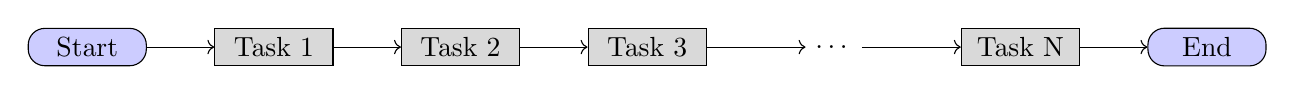
\begin{tikzpicture}[node distance=2.37cm]
      
    \node (start) [StartEndNode] {Start};
    \node (task1) [OperationNode, right of=start] {Task 1};
    \node (task2) [OperationNode, right of=task1] {Task 2};
    \node (task3) [OperationNode, right of=task2] {Task 3};
    \node (dots) [right of=task3] {\dots};
    \node (taskn) [OperationNode, right of=dots] {Task N};
    \node (end) [StartEndNode, right of=taskn] {End};
    
    \draw [->] (start) -- (task1);
    \draw [->] (task1) -- (task2);
    \draw [->] (task2) -- (task3);
    \draw [->] (task3) -- (dots);
    \draw [->] (dots) -- (taskn);
    \draw [->] (taskn) -- (end);
  \end{tikzpicture} \\ 
  \vspace{0.5cm} % Space between diagrams
  \textbf{Parallel Computing} \\
  \vspace{0.2cm}
  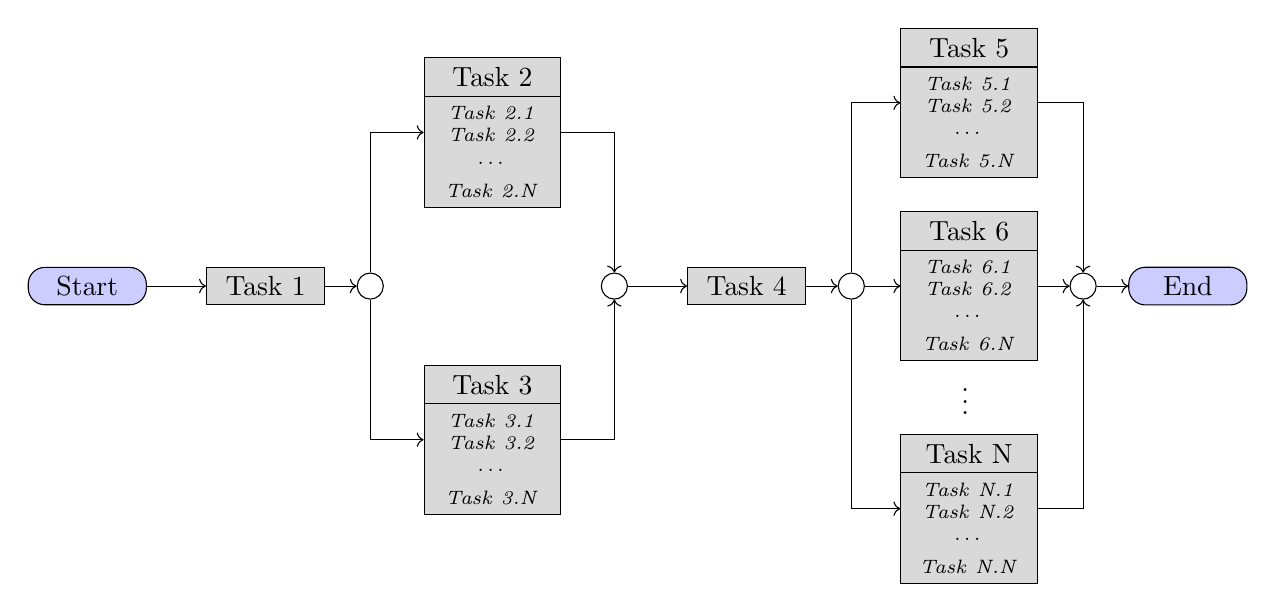
\begin{tikzpicture}[node distance=0.4cm]
    
    \node (start) [StartEndNode] {Start};
    \node (task1) [OperationNode, right=0.75cm of start] {Task 1};
    \node (ConnNode01) [ConnNode, right=of task1] {};
    \node (task2) [OperationNode, rectangle split, rectangle split parts=2, above right=0.75cm and 1.25cm of task1, text width=1.5cm, text centered] {
      Task 2
      \nodepart{two}{\scriptsize{\textit{Task 2.1}\\ \textit{Task 2.2}\\ \dots \\ \textit{Task 2.N}}}
    };
    \node (task3) [OperationNode, rectangle split, rectangle split parts=2, below right=0.75cm and 1.25cm of task1, text width=1.5cm, text centered] {
      Task 3
      \nodepart{two}{\scriptsize{\textit{Task 3.1}\\ \textit{Task 3.2}\\ \dots \\ \textit{Task 3.N}}}
    };
    \node (ConnNode02) [ConnNode, right=3.5cm of task1] {};
    \node (task4) [OperationNode, right=0.75cm of ConnNode02] {Task 4};
    \node (ConnNode03) [ConnNode, right=of task4] {};
    \node (task5) [OperationNode, rectangle split, rectangle split parts=2, above right=1.25cm and 0.5cm of ConnNode03, text width=1.5cm, text centered] {
      Task 5
      \nodepart{two}{\scriptsize{\textit{Task 5.1}\\ \textit{Task 5.2}\\ \dots \\ \textit{Task 5.N}}}
    };
    \node (task6) [OperationNode, rectangle split, rectangle split parts=2, right=0.45cm of ConnNode03, text width=1.5cm, text centered] {
      Task 6
      \nodepart{two}{\scriptsize{\textit{Task 6.1}\\ \textit{Task 6.2}\\ \dots \\ \textit{Task 6.N}}}
    };
    \node (dots) [below right=0.85cm and 1.15cm of ConnNode03] {\vdots};
    \node (taskn) [OperationNode, rectangle split, rectangle split parts=2, below right=1.75cm and 0.5cm of ConnNode03, text width=1.5cm, text centered] {
      Task N
      \nodepart{two}{\scriptsize{\textit{Task N.1}\\ \textit{Task N.2}\\ \dots \\ \textit{Task N.N}}}
    };
    \node (ConnNode04) [ConnNode, right=of task6] {};
    \node (end) [StartEndNode, right=of ConnNode04] {End};

    \draw [->] (start) -- (task1);
    \draw [->] (task1) -- (ConnNode01);
    \draw [->] (ConnNode01) |- (task2);
    \draw [->] (ConnNode01) |- (task3);
    \draw [->] (task2) -| (ConnNode02);
    \draw [->] (task3) -| (ConnNode02);
    \draw [->] (ConnNode02) -- (task4);
    \draw [->] (task4) -- (ConnNode03);
    \draw [->] (ConnNode03) |- (task5);
    \draw [->] (ConnNode03) -- (task6);
    \draw [->] (ConnNode03) |- (taskn);
    \draw [->] (task5) -| (ConnNode04);
    \draw [->] (task6) -- (ConnNode04);
    \draw [->] (taskn) -| (ConnNode04);
    \draw [->] (ConnNode04) -- (end);
  \end{tikzpicture}
  \caption[Diagram of serial and parallel computing]{\textbf{Diagram of serial and parallel computing.}}
  \label{fig:computing-strategies}
\end{figure}

Parallel computing marks a paradigm shift from traditional sequential approaches, employing multiple processors or computing units to simultaneously perform tasks. This paradigm has gained prominence in response to growing computational demands, especially with the increasing complexity of data volumes and problem-solving requirements. Early parallel systems were tightly coupled, sharing memory and closely coordinating tasks. The evolution of parallel computing architectures progressed from \ac{SIMD} to \ac{MIMD} systems, reflecting a shift towards greater flexibility and efficiency. Diverse parallel computing architectures are designed to meet specific computational needs. Shared-memory architectures, such as \ac{SMP}, enable processors to access a common memory pool. In contrast, distributed-memory architectures, seen in clusters or grids, involve processors with their dedicated memory. Hybrid architectures combine these models, capitalizing on the strengths of both shared and distributed memory systems \cite{matloff2012}.

One key metric in evaluating parallel computing performance is speedup (Eq. \ref{eq:speedup}), which is a relative measure used to analyze the efficiency gained by employing multiple processing elements compared to a single processor. The ideal speedup is linear, meaning that doubling the number of processing elements should ideally halve the computation time. However, achieving this ideal speedup is challenging, and many algorithms exhibit nearly linear speedup for a small number of processors, reaching an asymptotic behavior for a large number of processing elements \cite{grama2003,matloff2012}.

\begin{equation}
  S \colon (T_1, T_p) \mapsto \frac{T_1}{T_p} \in [0,\infty)
  \label{eq:speedup}
\end{equation}

\noindent where \(S\) is the speedup, \(T_1\) is the execution time on a single processor, \(T_p\) is the execution time on \(p\) processors.

This performance gain can be predicted by two models (Figure \ref{fig:laws-plot}): Amdahl's Law \cite{amdahl1967} and Gustafson's Law \cite{gustafson1988}. Amdahl's Law (Eq. \ref{eq:amdahl}), assumes the size of the computational problem is fixed, and the non-parallelizable fraction of the program is independent of the number of processors. Gustafson's Law (Eq. \ref{eq:gustafson}) addresses the deficiencies of Amdahl's Law, proposing that programmers tend to define the size of problems to exploit the computational power that becomes available as resources improve. In a way, Gustafson's Law redefines efficiency due to the possibility that limitations imposed by the sequential fraction of a program can be combated by an increase in available computational resources.

\begin{equation}
  S_A \colon (f_p, N_p) \mapsto \frac{1}{(1 - f_p) + \frac{f_p}{N_p}}
  \label{eq:amdahl}
\end{equation}

\begin{equation}
  S_G \colon (f_p, N_p) \mapsto (1 - f_p) + N_p \cdot f_p
  \label{eq:gustafson}
\end{equation}

\noindent where \(S_A\) is the speedup estimated by Amdahl's Law, \(S_G\) is the speedup estimated by Gustafson's Law, \(f_p\) is the parallelizable fraction of the code, and \(N_p\) is the number of available processors.

\begin{figure}[h]
  \centering
  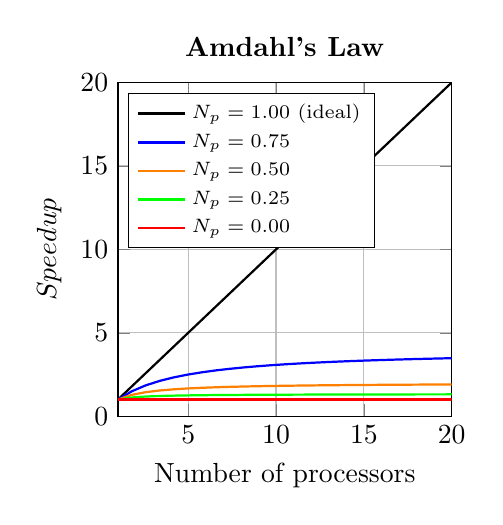
\begin{tikzpicture}
    \begin{axis}[
      xlabel={Number of processors},
      ylabel={$Speedup$},
      title=\textbf{Amdahl's Law},
      grid=major,
      xmin=1, xmax=20,
      ymin=0, ymax=20,
      height=0.48\textwidth, width=0.48\textwidth,
      domain=1:20,
      legend pos=north west,
      legend style={font=\scriptsize},
      legend cell align={left},
    ]
    \addplot[black, thick] {1 / ((1.0 - 1.0) + (1.0 / x))};
    \addlegendentry{$N_p=1.00$ (ideal)};
    \addplot[blue, thick] {1 / ((1.0 - 0.75) + (0.75 / x))};
    \addlegendentry{$N_p=0.75$};
    \addplot[orange, thick] {1 / ((1.0 - 0.5) + (0.5 / x))};
    \addlegendentry{$N_p=0.50$};
    \addplot[green, thick] {1 / ((1.0 - 0.25) + (0.25 / x))};
    \addlegendentry{$N_p=0.25$};
    \addplot[red, thick] {1 / ((1.0 - 0.0) + (0.0 / x))};
    \addlegendentry{$N_p=0.00$};
    \end{axis}
  \end{tikzpicture}
  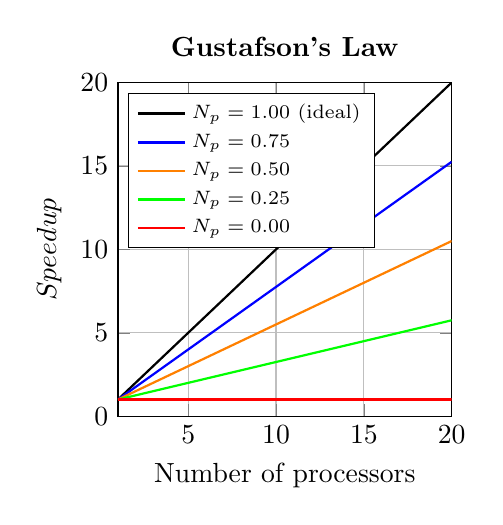
\begin{tikzpicture}
    \begin{axis}[
      xlabel={Number of processors},
      ylabel={$Speedup$},
      title=\textbf{Gustafson's Law},
      grid=major,
      xmin=1, xmax=20,
      ymin=0, ymax=20,
      height=0.48\textwidth, width=0.48\textwidth,
      domain=1:20,
      legend pos=north west,
      legend style={font=\scriptsize},
      legend cell align={left},
    ]
    \addplot[black, thick] {(1 - 1.0) + (1.0 * x)};
    \addlegendentry{$N_p=1.00$ (ideal)};
    \addplot[blue, thick] {(1 - 0.75) + (0.75 * x)};
    \addlegendentry{$N_p=0.75$};
    \addplot[orange, thick] {(1 - 0.5) + (0.5 * x)};
    \addlegendentry{$N_p=0.50$};
    \addplot[green, thick] {(1 - 0.25) + (0.25 * x)};
    \addlegendentry{$N_p=0.25$};
    \addplot[red, thick] {(1 - 0.0) + (0.0 * x)};
    \addlegendentry{$N_p=0.00$};
    \end{axis}
  \end{tikzpicture}
  \caption[Speedup according to Amdahl's and Gustafson's Laws]{\textbf{Speedup according to Amdahl's and Gustafson's Laws.} The speedup is presented as a function of the number of available processors for different fractions of parallelizable code ($N_p$), considering the estimates of Amdahl's and Gustafson's laws.}
  \label{fig:laws-plot}
\end{figure}

Following these rules, applications of parallel computing span various domains, from scientific simulations and data analytics to artificial intelligence. \ac{HPC} clusters address intricate scientific problems, such as simulating climate models, conducting molecular dynamics simulations for drug discovery, or analyzing large-scale genomics data. On the other hand, parallel processing significantly accelerates tasks like training machine learning models for image recognition, natural language processing, and recommendation systems. Additionally, parallel algorithms play a crucial role in speeding up tasks like sorting, searching, and graph traversal, contributing to improved efficiency in various computational domains. The future of parallel computing is influenced by ongoing advancements in hardware, software, and algorithms. Emerging technologies, such as quantum computing, introduce new dimensions to parallelism. Ongoing research explores novel ways to harness parallelism efficiently, overcome scalability challenges, and integrate parallel computing into mainstream applications. In summary, parallel computing stands as a cornerstone in addressing the escalating demands for computational power. Its comprehensive application ensures the development of efficient computational platforms for different research fields.

%%% Chapter 4: Data Coding in Structural Biology

\chapter{Data Coding in Structural Biology}

Data coding, in essence, refers to the process of representing information or data using a specific set of symbols, codes, or conventions. This encoding allows for the efficient storage, transmission, and processing of data. In computer science, data coding can involve various techniques, such as character encoding (representing characters with numerical values), binary coding (using combinations of 0s and 1s to represent information), and other methods tailored to specific types of data.

The data coding of biomolecules and binding sites plays a fundamental role in structural biology, enabling the computational representation, visualization and analysis of complex biological information \cite{kozlikova2016}. This process converts biological information into formats that are understandable and suitable for processing by algorithms and programs in computational systems. Data coding involves assigning numerical or categorical codes to biological components, \eg, atoms, amino acids, and nucleotides, to describe occupancy, coordinates, forces, physicochemical characteristics, and/or structural properties.

In structural biology, data coding is important for performing advanced analyses, \eg, molecular modeling, \ac{MD} simulations, and interaction prediction. There are several applications that exemplify the biological data coding for computational analyses. For instance, in molecular modeling, a protein can be coded using one-letter codes to represent different amino acids, as seen in protein sequence representation, to predict protein folding, as applied in ESMFold \cite{lin2022}, AlphaFold \cite{jumper2021} and RosettaFold \cite{baek2021}. In \acs{MD} simulation, the \acs{3D} coordinates of atoms or sets of atoms, along with vectors representing forces or other attributes, are used to represent the structure of a biomolecule, as in GROMACS \cite{gromacs} or AMBER \cite{amber} in atomistic-scale simulations and in CafeMol in coarse-grained molecular dynamics simulations \cite{kenzaki2011}. Additionally, binding sites, once identified by computational algorithms, are coded in different ways for further analyses. Binding sites can be coded to represent the spatial and physicochemical features of a biomolecular region, such as the \acs{3D} grids used in the KVFinder suite \cite{guerra2019,guerra2020,guerra2021,guerra2023B}, or the \acs{3D} coordinates of atoms, as in Fpocket \cite{fpocket}.

When working with computational models for the study of biomolecules, data coding is essential for the abstraction and computational representation of biological data. This abstraction is crucial for the development of computational tools aimed at studying biomolecular systems. Here, we present the data codings implemented for biomolecules and binding sites, \ie, volumetric representation, atomistic representation, and graph representation.

\section{Volumetric Representation}

Biomolecules and their binding sites can be represented in a \acs{3D} grid, organized into volumetric pixels, commonly known as voxels. This grid, akin to a matrix (\eg, a numpy array), assigns values to each voxel, encapsulating a discrete point of data within the \acs{3D} grid. Each voxel, acting as a discrete data point, can contain multiple types of information, enabling a straightforward and efficient representation of various properties within a specific portion of space (Figure \ref{fig:voxel}). In computer science, the \acs{3D} grid is a widely employed data structure in image processing and computer vision applications, including tasks such as image reconstruction, image segmentation, and object detection.

\begin{figure}[h]
  \centerline{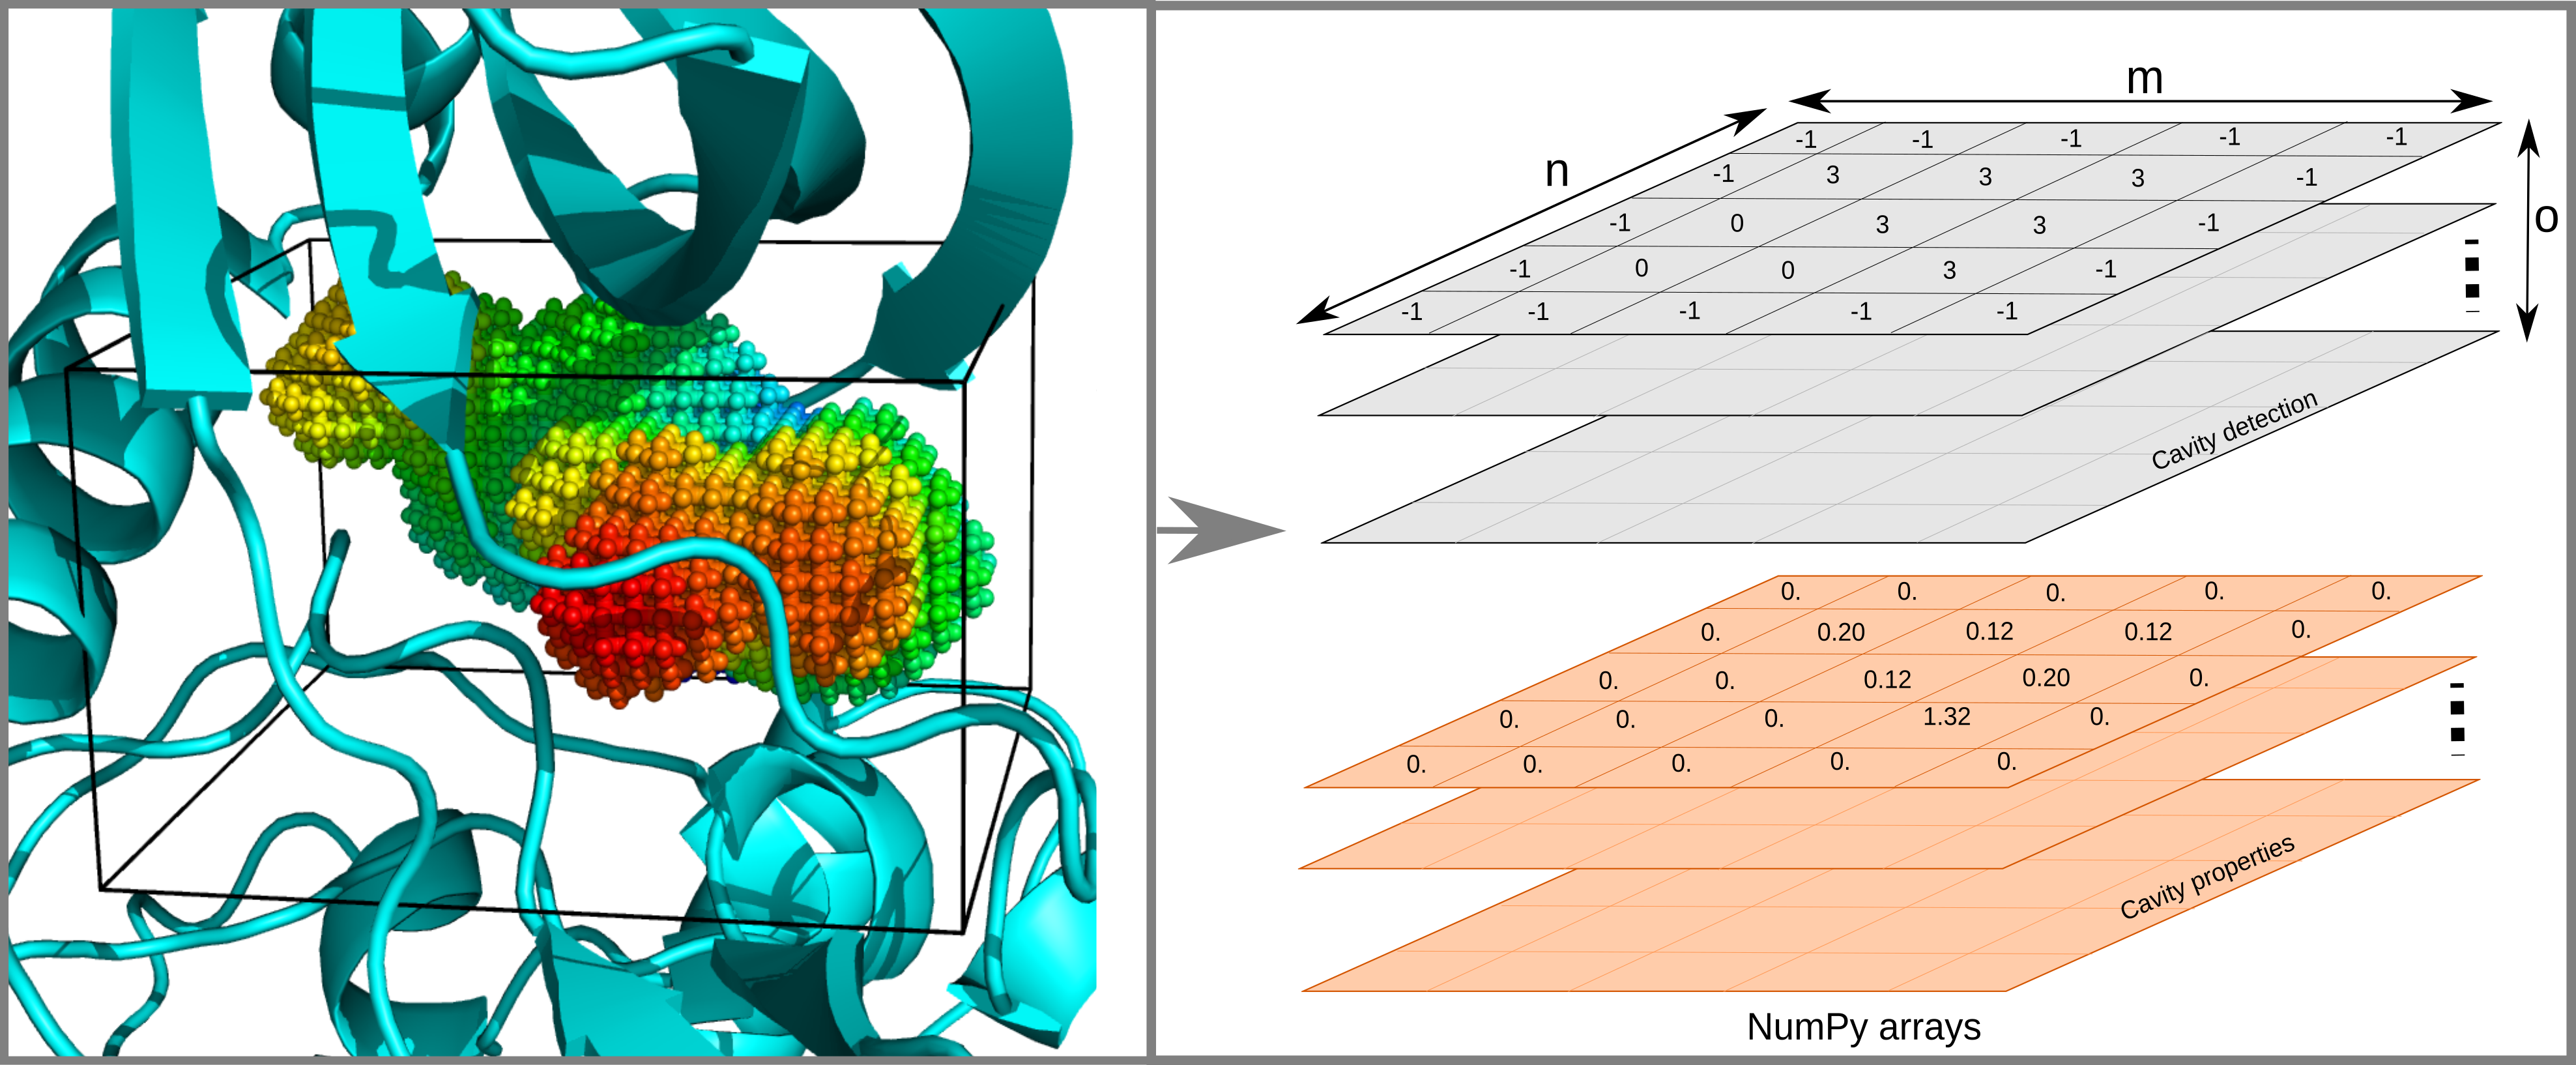
\includegraphics[scale=1]{images/voxels.png}}
  \centerline{\tiny{\textbf{Source:} Reprinted from \cite{guerra2021}. Licensed under \href{https://creativecommons.org/licenses/by/4.0/}{CC BY 4.0}.}}
  \caption[Grid representations]{\textbf{Grid representations.} Based on a 3D grid with dimensions (m, n, o), each element corresponds to a region of cavity (>1), empty space (1), biomolecule (0), or solvent (-1). Additionally, properties are stored in the same data structure, corresponding to the property value in the region.}
  \label{fig:voxel}
\end{figure}

Among various molecular surface representations, the \acs{3D} grid composed of voxels is the simplest and most suitable for representing multiple properties under various conditions, as each voxel in the \acs{3D} grid can store multiple information, \eg, charge distribution, burial extent (depth), hydrophobicity, hydrogen-bond-forming regions and cavity identifier. Moreover, the \acs{3D} grid is an efficient data structure for storing and accessing values and/or attributes at a \acs{3D} position, enabling the performance of mathematical and logical operations within a \acs{3D} region. Its versatility makes it an ideal choice for the development of computational algorithms, leveraging parallel computing techniques to accelerate the processing of large datasets.

The computational complexity of grid-based algorithms heavily relies on the input size, \ie, the number of voxels. Higher density grids offer a more detailed spatial representation, which proves beneficial for in-depth studies but comes at the cost of increased computational requirements, \ie, increased memory consumption and poorer time performance. For cavity detection algorithms, efficiency is often assessed based on the linear scalability of time complexity with the number of voxels, deeming exponential scalability inefficient. Within this context, the voxel clustering algorithm emerges as the most time-intensive step, primarily due to its limited parallelizability. 

In the parKVFiner software, the voxel length is a user-defined parameter, with default value of 0.6 Å. However, users have the flexibility to adjust this value based on the specific demands of their case studies. For instance, a smaller voxel length, such as 0.25 Å, is recommended for those seeking a more accurate morphological characterization of biomolecular cavities. The computational complexity is intricately tied to the number of voxels ($n_v$), denoted as $\mathcal{O}(n_v)$. User inputs determine the number of voxels (Eq. \ref{eq:nv}), calculated as follows:

\begin{equation}
  n_v \colon (l_x,l_y,l_z,Po,s) \mapsto \left \lceil \frac{l_x + 2 \cdot Po + s}{s} \right \rceil \cdot \left \lceil \frac{l_y + 2 \cdot Po + s}{s} \right \rceil \cdot \left \lceil \frac{l_z + 2 \cdot Po + s}{s} \right \rceil
  \label{eq:nv}
\end{equation}

\noindent where $l_x$, $l_y$, $l_z$ are the lengths of the target biomolecule along x, y, and z-axis, respectively, $Po$ is the \textit{Probe Out} size, $s$ is the grid spacing, and $\lceil \cdot \rceil$ is the ceiling function.

Under typical conditions, the average dimensions of the \acs{3D} grid, denoted as $(\bar{m},\bar{n},\bar{o})$, are roughly $(120,120,120)$, along the x, y, and z axes, respectively. The computational complexity increases as the region of interest, dictated by the biomolecule and the probe size, influences the number of voxels, where the voxel-level analysis, inherent to the algorithm, amplifies computational demands.

Turning to spatial complexity, the number of voxels and the bit-depth of grid elements significantly influence memory usage, with the latter also impacting precision. The choice between int (32-bit integer) and double (64-bit floating-point) in the C-coded parKVFinder reflects a balance between memory efficiency and the precision required for accurate calculations. Spatial complexity scales linearly with the number of voxels ($n_v$), denoted as $\mathcal{O}(n_v)$. In parKVFinder, the grid for cavity and surface points identifiers is an integer grid (32-bit integer), while cavity properties, such as point depth and hydrophobicity, are stored in a double grid (64-bit floating-point).

\subsection{Molecular Surface Representation}

The representation of molecular surfaces is a crucial step in the modeling and analysis of biomolecules. In this approach, biomolecules are described through a rigid sphere model, considering atomic positions and radii to represent the molecular surface. There are three commonly used mathematical formulations to represent molecular surfaces (Figure \ref{fig:surface-representation}):

\begin{enumerate}[label=\textbf{(\Alph*)}]
  \item \textbf{\acs{vdW} surface:} represents each atom as a sphere whose radius is proportional to its van der Waals radius. The \acs{vdW} surface is depicted as the union of these spherical atoms;
  \item \textbf{\acs{SAS}:} represents regions of a molecule that can be accessed by a solvent molecule (e.g., a water molecule), approximated by a spherical probe;
  \item \textbf{\acs{SES}:} is similar to \acs{SAS} but considers the outer shell of the probe instead of the probe's center.
\end{enumerate}
  
\begin{figure}[H]
  \centerline{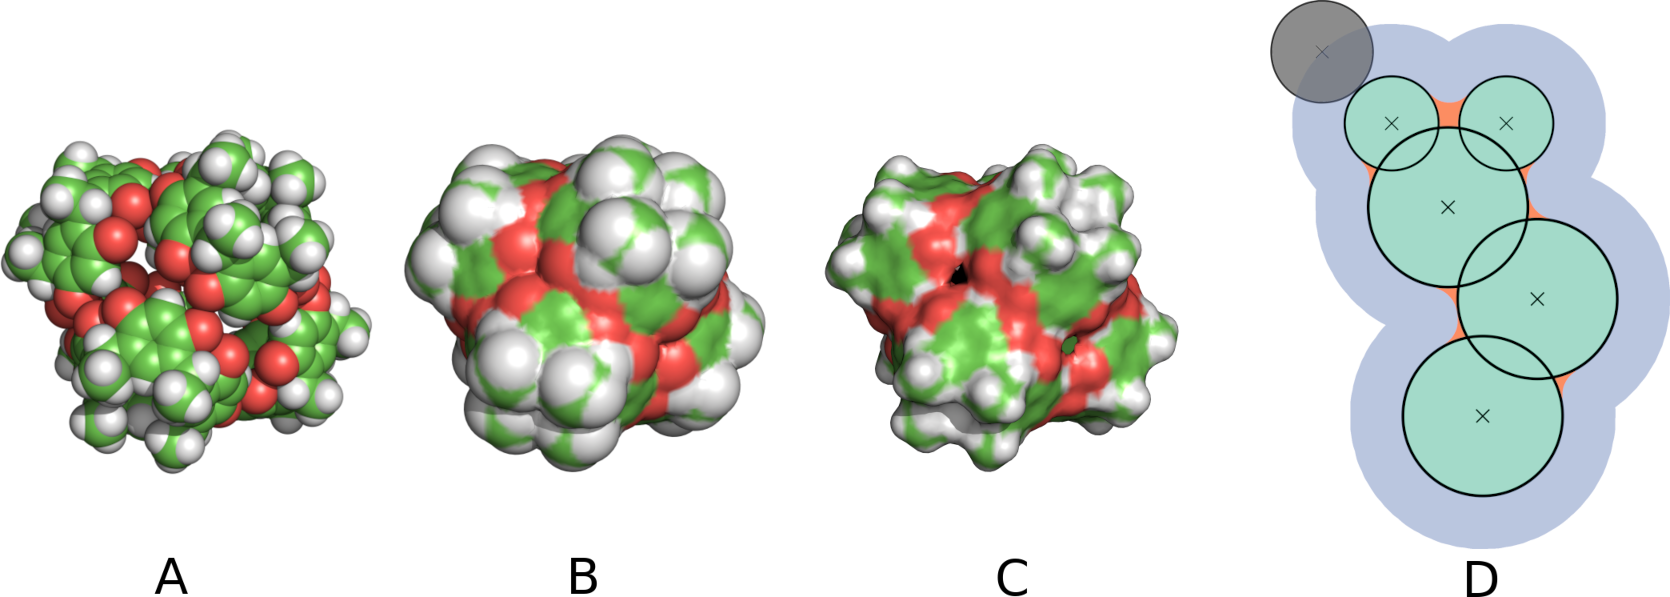
\includegraphics[scale=0.9]{images/surface-representation.png}}
  \centerline{\tiny{\textbf{Source:} Reprinted with permission from \cite{guerra2023B}. Copyright 2023 American Chemical Society.}}
  \caption[Molecular surface representations]{\textbf{Molecular surface representations.} \textbf{(A)} \acs{vdW} surface. \textbf{(B)} \acs{SAS}. \textbf{(C)} \acs{SES}. Images generated with PyMOL for the supramolecular cage (resorcin[4]arene-hexameric). \textbf{(D)} 2D schematic representation of molecular surfaces. The \acs{vdW} surface (green) consists of atoms represented as green spheres. A spherical probe (gray), representing a solvent molecule, rolls over the atoms of the molecule to define \acs{SES} and \acs{SAS}. \acs{SES} is defined by the \acs{vdW} surface (green) and the space not reached by the spherical probe (orange). \acs{SAS} is defined by the envelope reached by the center of the spherical probe (blue).}
  \label{fig:surface-representation}
\end{figure}

\section{Atomistic Representation}

In our exploration of structural and functional characterization, we now turn to atomistic representation, an alternative to the voxel-based approach. Rather than representing structural data through voxels in a \acs{3D} grid, biomolecules and their binding sites can also be portrayed through their atomistic representation (Figure \ref{fig:atomistic-representation}). This representations are applied in tools of molecular dynamics simulations, such as GROMACS \cite{gromacs}, AMBER \cite{amber}, and CafeMol \cite{kenzaki2011}. Here, atoms, residues, and/or nucleobases are modeled as hard sphere models in \acs{3D} coordinates (x, y, z), along with vectors (\eg, forces, velocities, and accelerations) and properties (\eg, mass, charge, and van der Waals radius).

\begin{figure}[h]
  \centerline{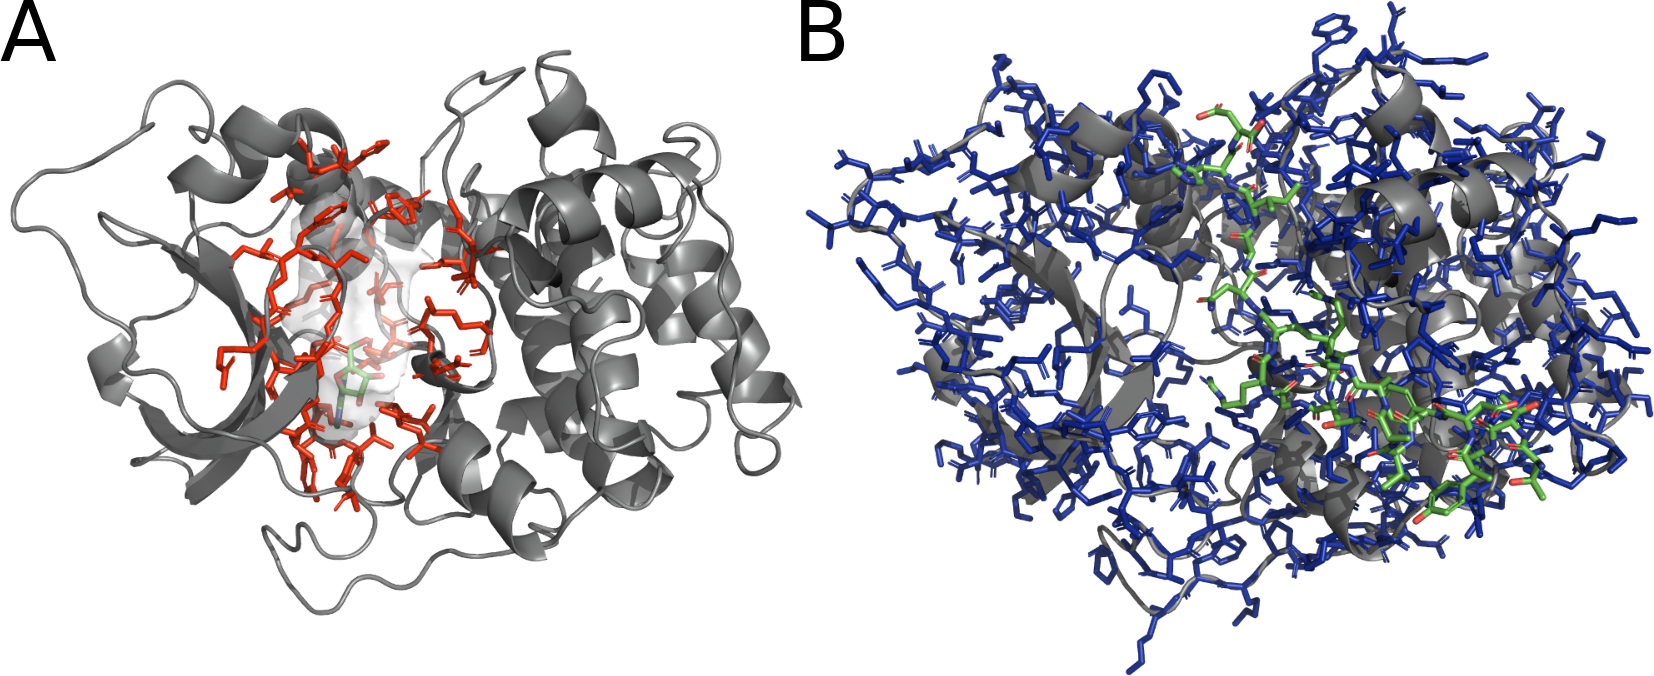
\includegraphics[scale=2]{images/atomistic-representation.png}}
  \caption[Atomistic representations]{\textbf{Atomistic representations.} \textbf{(A)} Atoms and amino acids (\textit{sticks} in green) forming the adenosine binding site (transparent surface). \textbf{(B)} Atoms and amino acids (\textit{sticks} in blue) exposed to the solvent, excluding binding sites for small molecules, with an inhibitor bound (\textit{sticks} in green). Images generated with PyMOL for a subunit of cyclic AMP-dependent protein kinase (PDB ID: 1FMO).}
  \label{fig:atomistic-representation}
\end{figure}

Yet, when delving effectively into interaction regions, a prerequisite emerges---the filtration of areas of interest, such as binding sites (Figure \ref{fig:atomistic-representation}A) or solvent-exposed regions (Figure \ref{fig:atomistic-representation}B). This atomistic representation allows precise and in-depth analysis, focusing on interactions and structural features relevant to biological function. Additionally, atomistic information can be utilized in molecular docking studies, rational drug design, and prediction of molecular interactions. These applications significantly contribute to the development of new therapeutic compounds and aid in understanding the molecular mechanisms involved in biological processes.

Parallel to the challenges encountered in volumetric representation, the computational complexity of algorithms based on atomistic representations hinges on the input size---specifically, the number of atoms. Researchers must balance the level of detail required for their analyses with the computational resources available, opting for fine-grained (all-atom), coarse-grained or carbon\textalpha\space (backbone) models. Spatial complexity is linearly dependent on the number of atoms ($n_a$), denoted as $\mathcal{O}(n_a)$. 

Within parKVFinder, the atomistic representation encodes each atom by its residue number (32-bit integer), chain identifier (char), residue name (4-char array), atom type (char), coordinates (64-bit floating-point), and \acs{vdW} radius (64-bit floating-point). Concurrently, interface residues are represented by residue number (32-bit integer), chain identifier (char) and residue name (4-char array). In both instances, spatial complexity significantly diminishes compared to volumetric representation, given the fewer atoms or interface residues compared to voxels for the same target biomolecule. When applying atomistic representation, researchers adopt the biomolecule's perspective, in contrast to the cavity point-of-view inherent in volumetric representation.

\section{Graph Representation \label{sec:graph-representation}}

Expanding upon the atomistic representation, the utilization of graph-based models emerges as a robust representation for examining interactions and relationships within biomolecules. Graph theory techniques are widely applied across diverse scientific domains such as biology, chemistry, physics, computer science, and mathematics \cite{foulds1995, majeed2020}. A cornerstone in discrete mathematics, it models the relationships and interactions between objects in a network, assisting in the analysis of biological interaction networks at various scales. In structural biology, graph theory has been utilized to investigate the structure, folding, stability, function, allostery and dynamics of proteins \cite{vishveshwara2002,dipaola2015,heal2018,kantelis2022}.

A graph $\mathcal{G(V,E)}$ (Figure \ref{fig:graph-examples}) is a mathematical structure, where $\mathcal{V} = \{v_1, v_2, \dots, v_n\}$ is a nonempty, finite set of vertices (also known nodes, point and junction), and $\mathcal{E} = \{e_1, e_2, \dots, e_n\}$ is a set of unordered pairs of distinct vertices of $\mathcal{V}$, whose elements $\{v_i,v_j\} \in \mathcal{E}$, where $v_i,v_j \in \mathcal{V}$, connects vertices $v_i$ and $v_j$ and termed edges (also known as line, arc, branch and link). Graphs can be directed (also known as digraph), where edges link two vertices symmetrically, or undirected, where edges link two vertices asymmetrically. Additionally, graphs can also be weighted, where each edge is assigned a weight or cost, which can represent a physical distance, a similarity measure, or any other property \cite{foulds1995,bondy1976,majeed2020,black2020}. Evolving from this, graph theory finds applications in modeling biological and chemical systems. In chemistry, molecular graphs capture the structural relationships between atoms and bonds, facilitating the study of chemical compounds and reactions. Biomolecules, which are assemblies of atoms (vertices) connected by intramolecular and intermolecular interactions (edges), have also been extensively explored through graph theory \cite{vishveshwara2002,mason2007}.

\begin{figure}[h]
  \centering
  \begin{subfigure}{0.32\textwidth}
    \centering
    \textbf{\footnotesize{Undirected graph}}
    \vspace{0.25cm} \\
    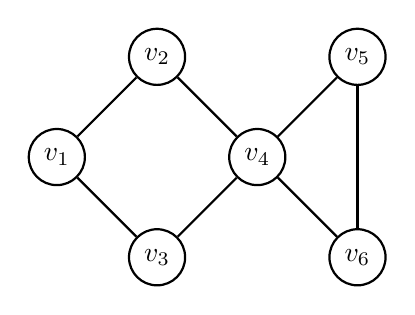
\begin{tikzpicture}[node distance={18mm}, thick]
      \node[ConnNode] (1) {$v_1$}; 
      \node[ConnNode] (2) [above right of=1] {$v_2$}; 
      \node[ConnNode] (3) [below right of=1] {$v_3$}; 
      \node[ConnNode] (4) [above right of=3] {$v_4$}; 
      \node[ConnNode] (5) [above right of=4] {$v_5$}; 
      \node[ConnNode] (6) [below right of=4] {$v_6$}; 
      \draw (1) -- (2); 
      \draw (1) -- (3); 
      \draw (2) -- (4); 
      \draw (3) -- (4);
      \draw (4) -- (5);
      \draw (4) -- (6);
      \draw (5) -- (6);
    \end{tikzpicture}
  \end{subfigure}
  \hfill
  \begin{subfigure}{0.32\textwidth}
    \centering
    \textbf{\footnotesize{Directed graph}}
    \vspace{0.25cm} \\
    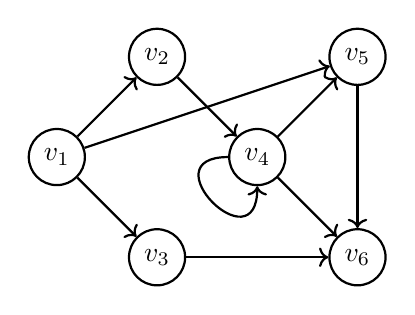
\begin{tikzpicture}[node distance={18mm}, thick]
      \node[ConnNode] (1) {$v_1$}; 
      \node[ConnNode] (2) [above right of=1] {$v_2$}; 
      \node[ConnNode] (3) [below right of=1] {$v_3$}; 
      \node[ConnNode] (4) [above right of=3] {$v_4$}; 
      \node[ConnNode] (5) [above right of=4] {$v_5$}; 
      \node[ConnNode] (6) [below right of=4] {$v_6$};
      \draw[->] (1) -- (2); 
      \draw[->] (1) -- (3);
      \draw[->] (1) -- (5); 
      \draw[->] (2) -- (4); 
      \draw[->] (3) -- (6);
      \draw[->] (4) to [out=180,in=270,looseness=5] (4); 
      \draw[->] (4) -- (5);
      \draw[->] (4) -- (6);
      \draw[->] (5) -- (6);
    \end{tikzpicture}
  \end{subfigure}
  \hfill
  \begin{subfigure}{0.32\textwidth}
    \centering
    \textbf{\footnotesize{Weighted graph}}
    \vspace{0.25cm} \\
    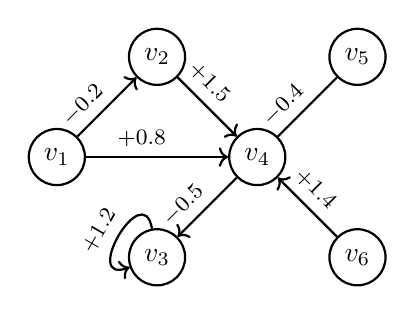
\begin{tikzpicture}[node distance={18mm}, thick]
      \node[ConnNode] (1) {$v_1$}; 
      \node[ConnNode] (2) [above right of=1] {$v_2$}; 
      \node[ConnNode] (3) [below right of=1] {$v_3$};
      \node[circle] (Aux3) [above left=0.2cm and 0cm of 3, rotate=60] {\footnotesize{$+1.2$}}; 
      \node[ConnNode] (4) [above right of=3] {$v_4$}; 
      \node[ConnNode] (5) [above right of=4] {$v_5$}; 
      \node[ConnNode] (6) [below right of=4] {$v_6$};
      \draw[->] (1) -- node[midway, above right, sloped, pos=-0.1] {\footnotesize{$-0.2$}} (2);
      \draw[->] (1) -- node[midway, above right, sloped, pos=0.15] {\footnotesize{$+0.8$}} (4);
      \draw[->] (2) -- node[midway, above right, sloped, pos=-0.1] {\footnotesize{$+1.5$}} (4);
      \draw[->] (3) to [out=100,in=200,looseness=3] (3); 
      \draw[->] (4) -- node[midway, above right, sloped, pos=1.1] {\footnotesize{$-0.5$}} (3);
      \draw (5) -- node[midway, above right, sloped, pos=1.1] {\footnotesize{$-0.4$}} (4);
      \draw[->] (6) -- node[midway, above right, sloped, pos=1] {\footnotesize{$+1.4$}} (4); 
    \end{tikzpicture}
  \end{subfigure}
  \caption[Pictorial overview of graphs $\mathcal{G(V,E)}$]{\textbf{Pictorial overview of graphs $\mathcal{G(V,E)}$.}}
  \label{fig:graph-examples}
\end{figure}

In this context, we introduce a graph-based representation for biomolecules using the \acs{3D} coordinates (x, y, z) of a biomolecular structure or complex that generates a residue-level graph, where vertices represent residues and edges represent interactions or some type of relationship between them. The construction of edges is based on customizable distance cutoffs between atoms, such as \ac{CA}, \ac{CB}, or any other atom, which can be defined by the user (Figure \ref{fig:graph-representation}). According to \ac{CAPRI} Round 28 \cite{capri,round28}, a distance cutoff of 8 Å between any two \acs{CB} atoms (or \acs{CA} for Gly) define interface residues, and a distance cutoff of 4 Å between any two atoms define native contacts. Expanding on the \acs{CB} definition, a distance cutoff of 10 Å between any two \acs{CA} atoms to define interface residues. Thus, the default parameters set in the implementation are these distance cutoffs, establishing relationships or interactions between residues \cite{vishveshwara2002,mason2007}. Figure \ref{fig:graph-representation}A shows an example of a residue-level graph generated from an adenosine binding site (Figure \ref{fig:atomistic-representation}A), and Figure \ref{fig:graph-representation}B shows an example of a residue-level graph generated from a solvent-exposed surface (Figure \ref{fig:atomistic-representation}B).

\begin{figure}[H]
\centerline{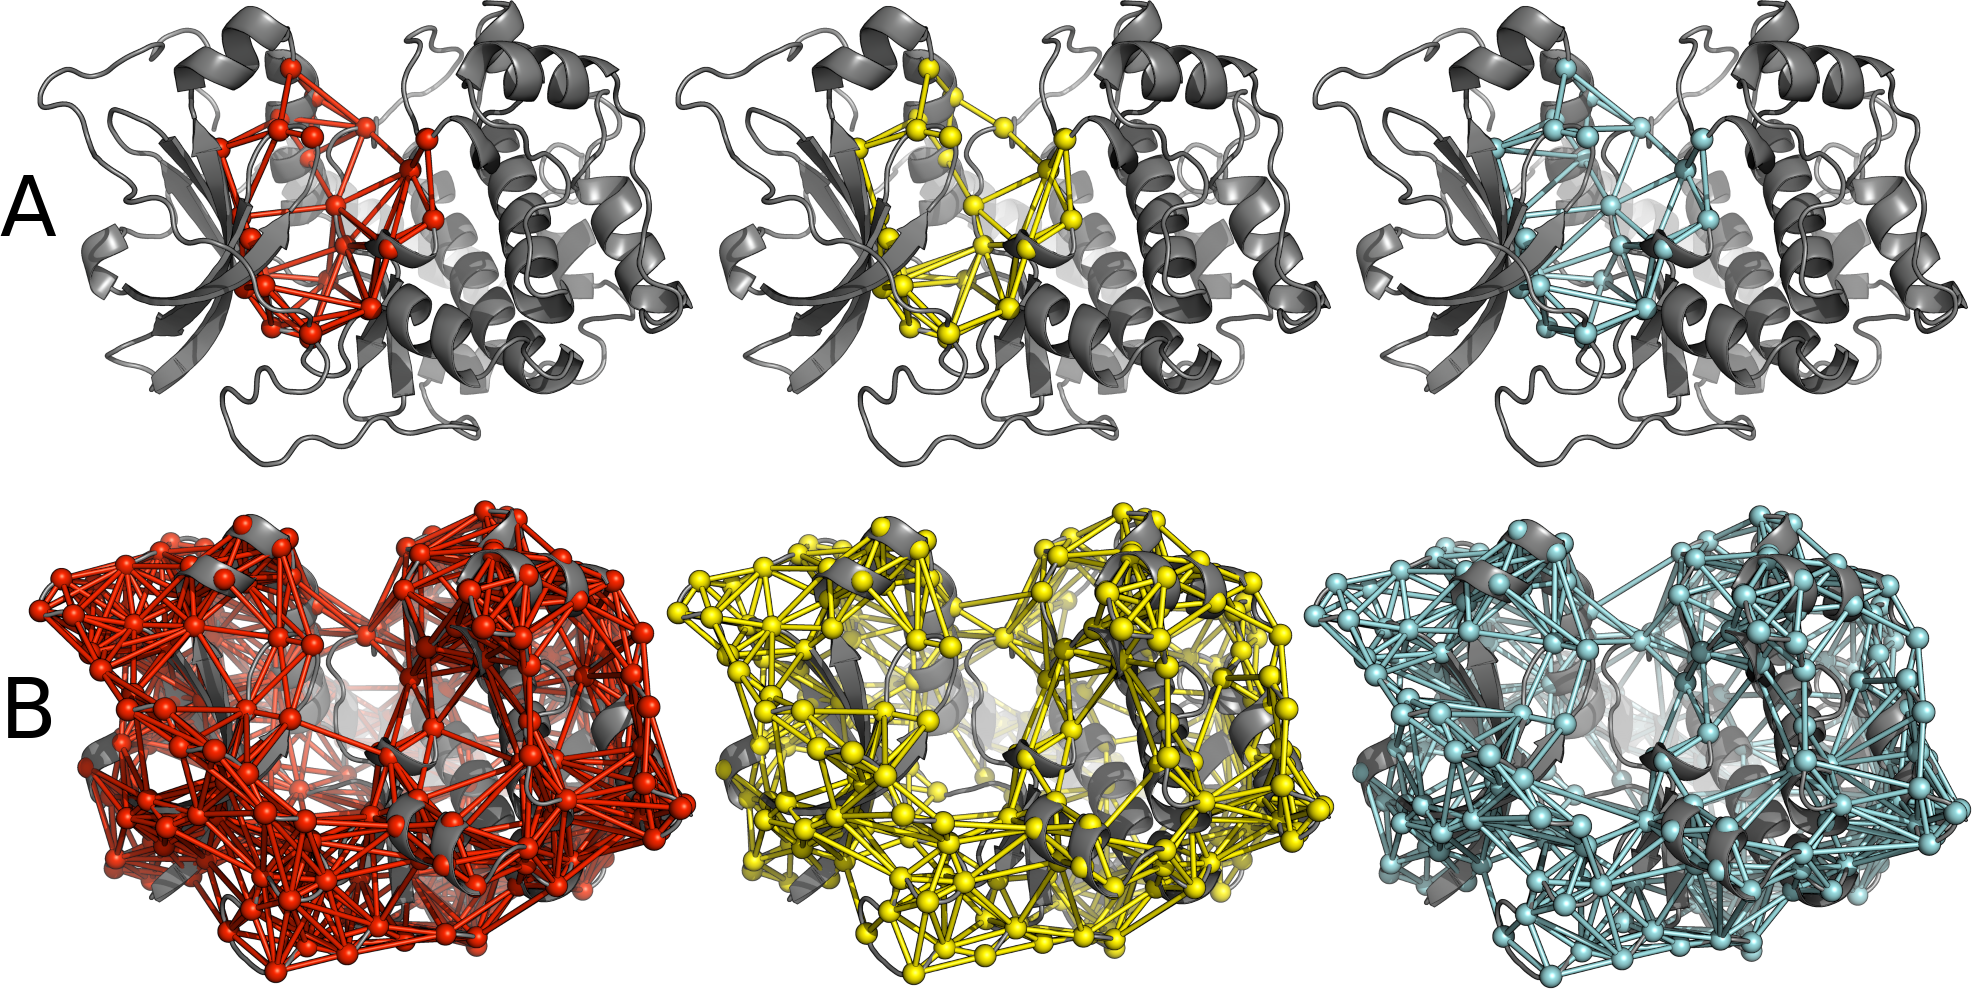
\includegraphics[scale=1.5]{images/graph-representation.png}}
\caption[Graph representations]{\textbf{Graph representations.} \textbf{(A)} Adenosine binding site as graphs with edges based on the distance cutoff of \acs{CA} (spheres and sticks in red), \acs{CB} (spheres and sticks in yellow), and any atoms of the residues (spheres and sticks in cyan). \textbf{(B)} Solvent-exposed surface, excluding binding sites for small molecules, as graphs with edges based on the distance cutoff of \acs{CA} (spheres and sticks in red), \acs{CB} (spheres and sticks in yellow), and any atoms of the residues (spheres and sticks in cyan). Images generated with PyMOL for a subunit of cyclic AMP-dependent protein kinase (PDB ID: 1FMO).}
\label{fig:graph-representation}
\end{figure}

This graph-based representation allows a more efficient analysis of interactions and relationships between residues, providing a visually intuitive exploration of the structural and functional attributes of the biomolecule. Additionally, various properties and metrics can be calculated from the graphs, such as paths, distances, centrality, and other metrics that aid in understanding the structure and function of the biomolecule \cite{majeed2020,vishveshwara2002,mason2007}. Since our primary focus is on the adjacency matrix, spatial complexity depends on the square of the number of vertices (\ie, number of residues---$n_r$), denoted as $\mathcal{O}(n_{r}^{2})$. However, as we include attributes (weights) on vertices and edges, spatial complexity will depend on the size of this additional data. With this graph-based representation in hand, novel mathematical approaches from graph theory can be applied to deepen our understanding of biological function and provide crucial insights for the development of therapies and therapeutic interventions.

%%% Chapter 5: KVFinder suite

% https://cnpemcamp-my.sharepoint.com/:w:/r/personal/joao_guerra_lnbio_cnpem_br/_layouts/15/Doc.aspx?sourcedoc=%7BD0C80180-AF7E-412F-B94E-6C38D8D4C946%7D&file=Relat%C3%B3rio%20Plataforma%20Biologia%20Computacional%202022.2.docx&action=default&mobileredirect=true


\chapter{KVFinder suite \label{ch:kvfinder-suite}}

The interactions between biomolecules play a crucial role in biological processes, involving entities ranging from small molecules such as ions and drugs to macromolecules such as proteins and nucleic acids. These receptor-ligand interactions (\eg, IPPs, IPLs, IPRs, and IPDs) take place at specific binding sites, which can be solvent-exposed clefts or cavities buried within the receptors. Morphological, topological, and physicochemical complementarity between ligands and receptors governs molecular recognition, limiting efficient interaction to a finite number of ligands. The identification and assessment of these regions are fundamental for understanding the tertiary structure of biomolecules and for the development of new drugs. To meet this demand, we have developed the computational platform \textbf{KVFinder suite}, which combines precise tools with high-performance processing, enabling the analysis of biomolecular experimental data and the comprehension of the biomolecular structure and function in biological systems.

The KVFinder suite consists of five computational tools that offer comprehensive functionalities for structural analysis and the study of biomolecular interactions. The tools included in the platform are: parKVFinder \cite{guerra2019,guerra2020}, pyKVFinder \cite{guerra2021}, KVFinder-web \cite{guerra2023A}, SERD, and KVFinderMD. Next, we will describe each of these tools, their main features, and their guideline applications.

\section{parKVFinder \label{sec:parkvfinder}}

The \ac{parKVFinder} \cite{guerra2020} is an open-source tool, licensed under GPL v3.0, developed for the detection and characterization of any type of biomolecular cavity. Originating from the master's thesis entitled "Prospecção e caracterização de cavidades supramoleculares" \cite{guerra2019}, it presents itself as an refactored, optimized and parallelized successor of KVFinder \cite{oliveira2014}. The initial release, parKVFinder \href{https://github.com/LBC-LNBio/parKVFinder/releases/tag/v1.0}{v1.0}, was published in \textit{SoftwareX} \cite{guerra2020}, with morphological (\ie, shape, volume, and area) and constitutional (\ie, interface residues surrounding cavities) characterizations. A notable addition was a novel algorithm for surface area estimation, based on Mullikin & Verbeek voxel classification. Progressing further, parKVFinder \href{https://github.com/LBC-LNBio/parKVFinder/releases/tag/v1.2.0}{v1.2.0} expanded its capabilities with additional morphological (\ie, depth), physicochemical (\ie, Eisenberg & Weiss hydrophobicity \cite{eisenberg1984}), and constitutional (\ie, residue frequency) characterizations \cite{guerra2023A}. 

The parKVFinder software is integrated with the PyMOL molecular viewer \cite{pymol} through a graphical plugin. The original plugin, PyMOL parKVFinder Tools, was developed for PyMOL v1.8 \cite{guerra2019,guerra2020}. However, with the advent of PyMOL v2.0 by Schröndinger, which discontinued support for the 1.8 version, a new plugin was developed---PyMOL2 parKVFinder Tools (Figure \ref{fig:pymol2-parkvfinder-tools}), written in Python3 with Qt interface. This update plugin incorporates new characterizations (depth and Eisenberg & Weiss hydrophobicity) from parKVFinder v1.2.0. This new plugin provides an intuitive and easy-to-use \ac{GUI}, allowing users to customize parameters for the detection and characterization of cavities.  Additionally, users can visualize identified cavities and their characteristics directly within the PyMOL environment (Figure \ref{fig:pymol2-parkvfinder-tools-visualization}). Alongside the \acs{GUI}, parKVFinder also serves advanced users with a \ac{CLI}, enabling task automation and program integration. The source code for parKVFinder and the PyMOL plugins is publicly available in the following repository: \url{https://github.com/LBC-LNBio/parKVFinder}.

\begin{figure}
  \centering
  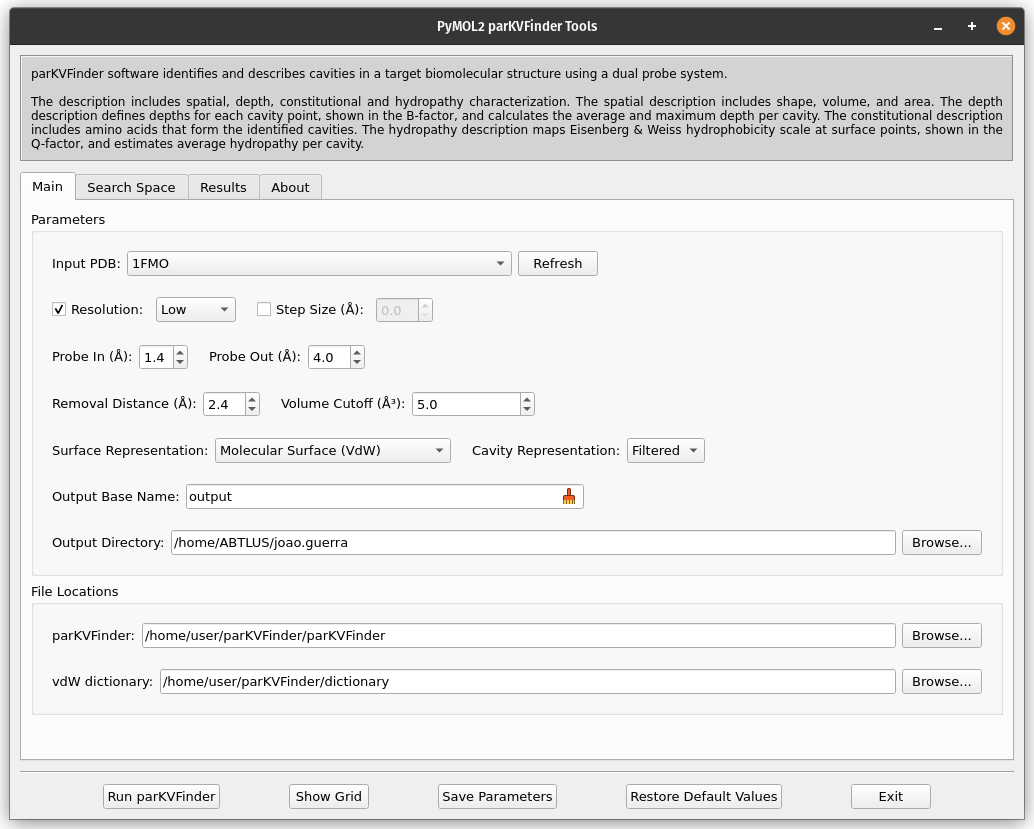
\includegraphics[scale=0.35]{images/pymol2-parkvfinder-tools.png}
  \caption[PyMOL2 parKVFinder Tools]{\textbf{PyMOL2 parKVFinder Tools.} The \textit{Main} tab presents the options that directly control the cavity detection procedure, in which user can set \textit{Probe In} and \textit{Probe Out} sizes, grid spacing, removal distance, volume filter, surface representation and cavity representation. Space segmentation features are managed in the \textit{Search Space} tab, allowing users to designate either the entire structure or custom search spaces. In box adjustment mode, an interactive box is drawn in the PyMOL viewer. Additionally, users can opt for ligand adjustment, limiting the search space around a defined ligand (PyMOL object) to a user-specified radius. After running parKVFinder, results (volume, surface area, depth, hydropathy, and interface residues) are interactively accessible in the \textit{Results} tab, and the cavity PDB file seamlessly loads into the PyMOL viewer.}
  \label{fig:pymol2-parkvfinder-tools}
\end{figure}

\begin{figure}[ht]
  \centering
  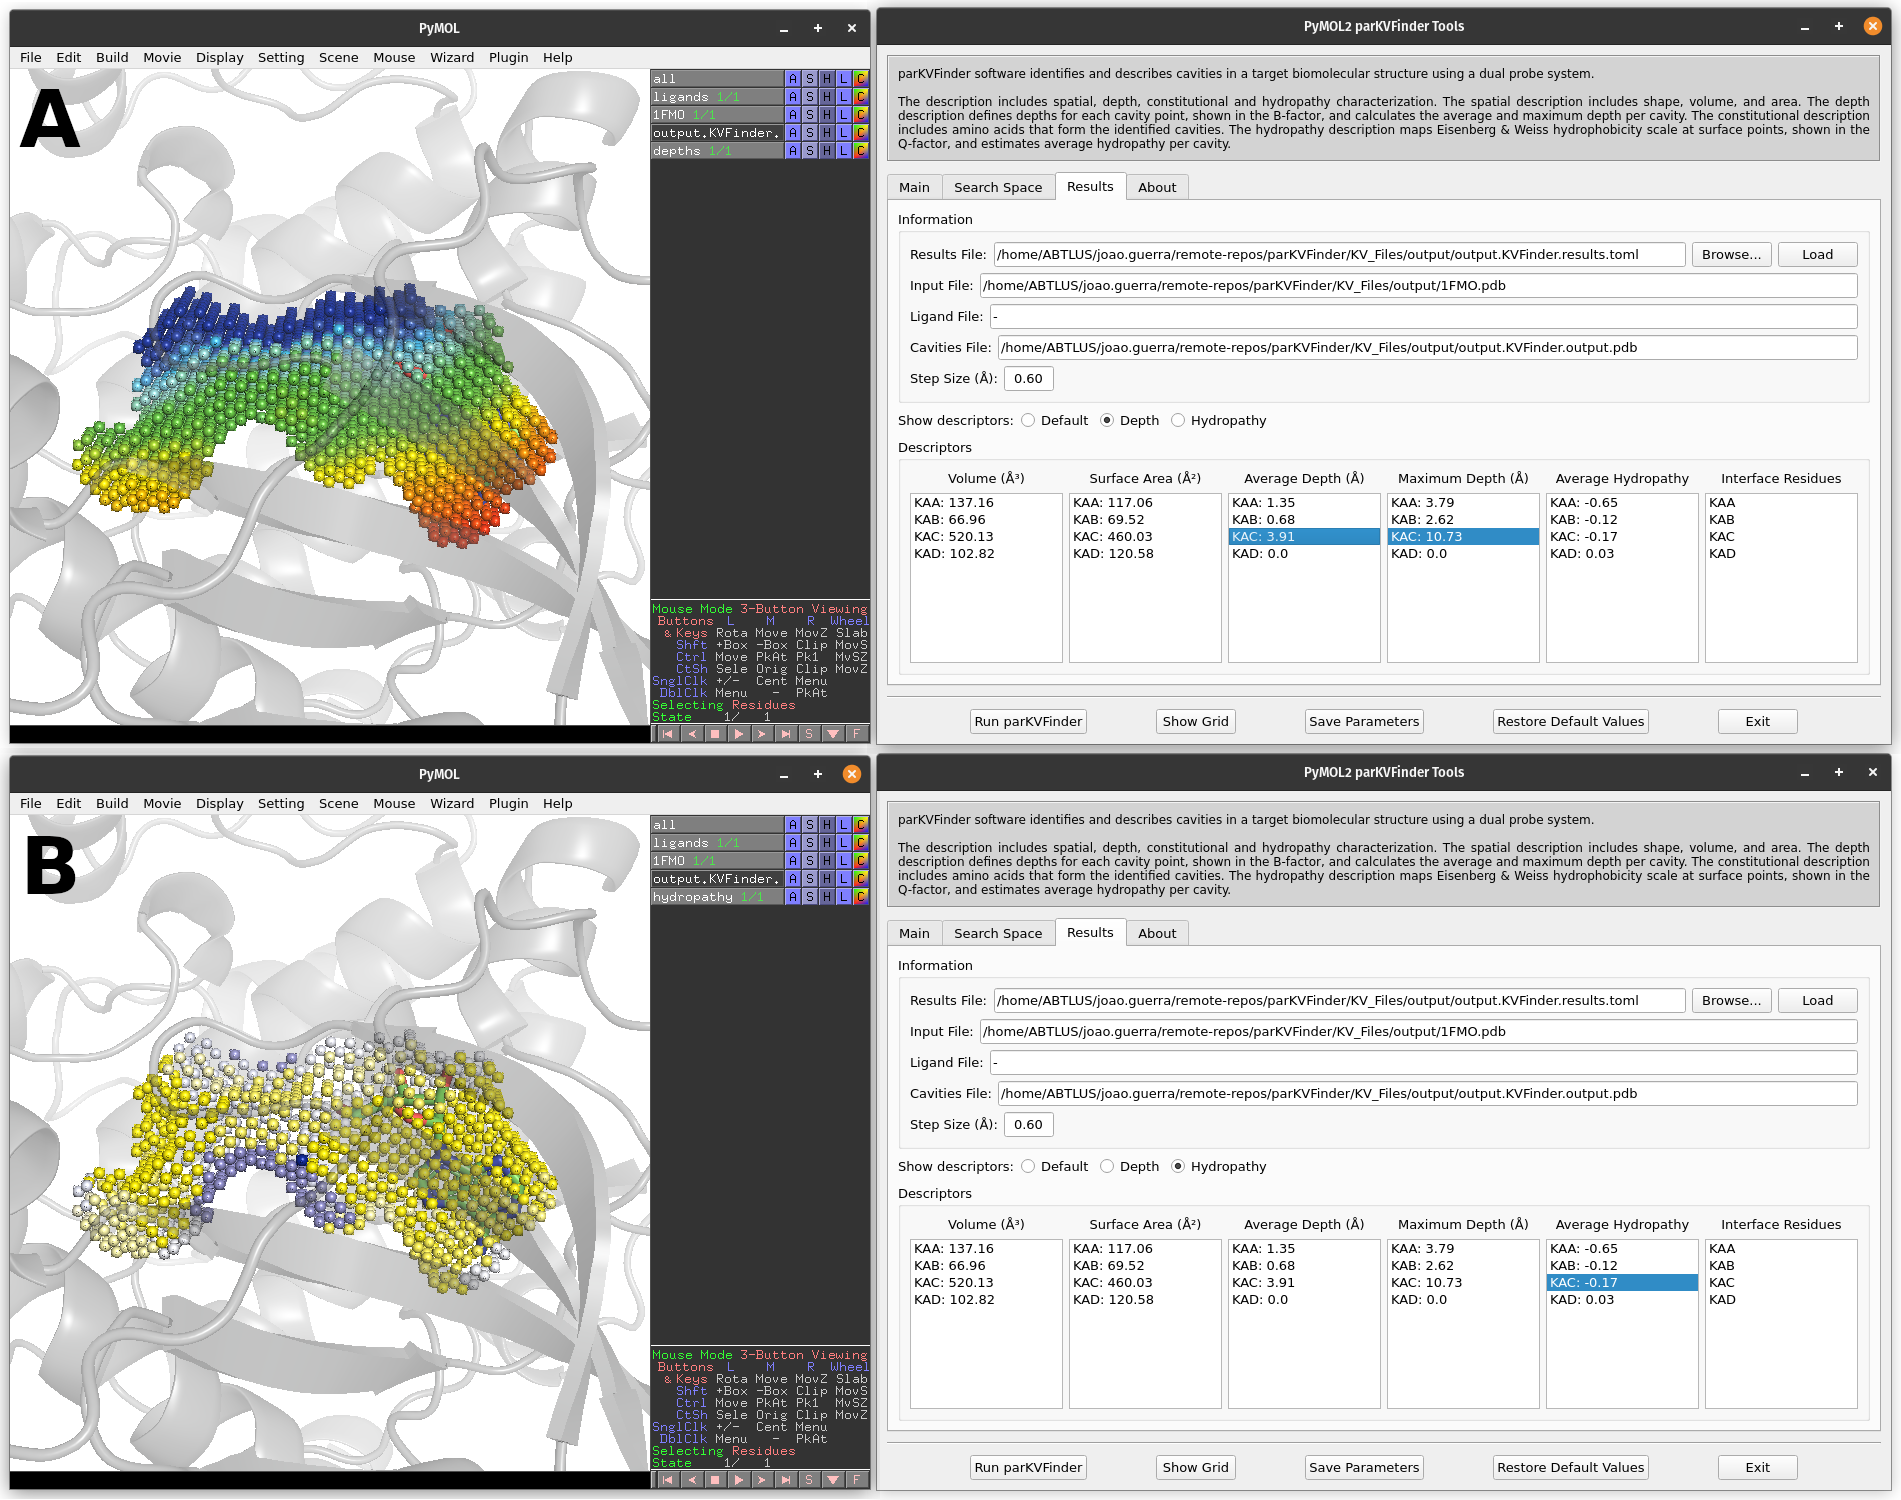
\includegraphics[scale=1]{images/pymol2-parkvfinder-tools-visualization.png}
  \caption[Interactive view of PyMOL2 parKVFinder Tools in PyMOL]{\textbf{Interactive view of PyMOL2 parKVFinder Tools in PyMOL.} Cavity characterization of the adenosine binding site in a protein kinase A (PDB ID: 1FMO). \textbf{(A)} Depth characterization: cavity points are colored by depth, ranging from superficial (blue points) to buried (red points). \textbf{(B)} Hydropathy characterization: surface cavity points are colored by Eisenberg & Weiss hydrophobicity scale, from $-1.42$ (highly hydrophobic) to $2.6$ (highly hydrophilic).}
  \label{fig:pymol2-parkvfinder-tools-visualization}
\end{figure}

Cavity detection and characterization routines in parKVFinder leverage the OpenMP library for parallelization, optimizing performance on multicore systems. Computational assessments on a set of 1000 protein domains (kv1000, \url{https://github.com/jvsguerra/kv1000}) revealed significant runtime reductions compared to KVFinder. The code optimization yielded a speedup of $\sim$1.5 times \cite{guerra2019} compared to KVFinder, and the subsequent code parallelization in parKVFinder led to a speedup of $\sim$6.5 times \cite{guerra2020}. Overall, parKVFinder demonstrated a remarkable $\sim$9.5 times reduction in runtime compared to KVFinder \cite{guerra2019,guerra2020}.

\subsection{Case Studies}

The parKVFinder was applied in two case studies published in scientific journals to investigate proteins of therapeutic interest. These analyses explored the dynamics of the flaps of the \ac{HIV-1} protease \cite{guerra2020} and the hydrophobicity profile of binding sites in alphaviruses \cite{ribeiro2021}. Next, we will describe each of these case studies in detail.

\subsubsection{Molecular Dynamics of HIV-1 Protease \label{sec:md-hiv1-protease}}

The active site of the HIV-1 protease represents a relevant therapeutic target for various antiretroviral drugs. This binding site exhibits significant complexity, which arises from the movement of \textbeta-hairpins, known as flaps, leading to structural and morphological variations. The volume of the binding site changes with the motion of these flaps, influencing substrate accessibility to the active site of the homodimer \cite{lam1994,soares2016}.

In this study, the \acs{MD} of the HIV-1 protease was investigated by identifying and evaluating the active site's volume during \acs{MD} simulations. Our objective was to describe the dynamic movement of the flaps through the volume and shape of the active site cavity as conformational descriptors in \acs{MD} simulations. To achieve this, 200 ns \acs{MD} simulations were conducted using the GROMACS 2019.4 package \cite{gromacs}, the AMBER99SB-ws force field, and the TIP42005s water model. The simulations initiated from the crystallographic structure of HIV-1 protease in the closed conformation \cite{lam1994}, excluding the inhibitor present in the structure, cyclic urea.

\begin{figure}[h]
  \centerline{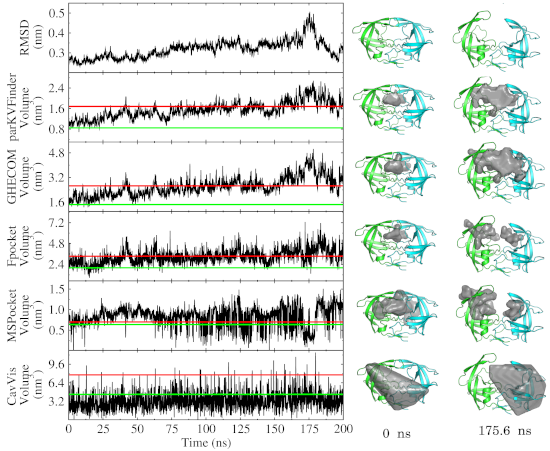
\includegraphics[scale=1.2]{images/hiv1-protease-md-analysis.png}}
  \centerline{\tiny{\textbf{Source:} Reprinted from \cite{guerra2020}. Licensed under \href{https://creativecommons.org/licenses/by/4.0/}{CC BY 4.0}.}}
  \caption[Volume of the HIV-1 protease active site over a 200 ns molecular dynamics simulation]{\textbf{Volume of the HIV-1 protease active site over a 200 ns molecular dynamics simulation.} The green and red lines indicate the cavity volume for the closed (PDB ID: 1HVR) and semi-open (PDB ID: 1HHP) states, respectively. Protein structures at the beginning of the simulation (0 ns) and the frame with the highest \acs{RMSD} (175.6 ns) are shown as cartoons. The corresponding cavities detected by each tool are displayed as gray surfaces.}
  \label{fig:hiv1-protease-dm-analysis}
\end{figure}

The active site volume was monitored throughout the \acs{MD} simulations (Figure \ref{fig:hiv1-protease-dm-analysis}). Initially, the cavity volume corresponds to the closed conformation (green line). After $\sim$25 ns, it increases, reaching the value corresponding to the semi-open conformation (red line) around 75 ns, indicating an opening process. Subsequently, the flaps separate further, and the cavity achieves its maximum volume at $\sim$175 ns before reverting to the more stable semi-open conformation. This dynamic volume change correlates well (Pearson correlation; $\rho=0.72$) with the \ac{RMSD} of the \acs{CA} calculated from the closed conformation, providing an accurate depiction of the protein's conformational state throughout the simulation. It is noteworthy that \acs{RMSD} describes global structural variations, while the estimated volume offers a direct metric of conformational changes in the active site, possibly associated with ligand accessibility.

The performance of parKVFinder \cite{guerra2020} was benchmarked against other geometry-based methods (Figure \ref{fig:hiv1-protease-dm-analysis}), including GHECOM \cite{ghecom}, Fpocket \cite{fpocket}, MSPocket \cite{mspocket}, and CavVis \cite{cavvis}. The correlation between the estimated volume by each program and the \acs{RMSD} was evaluated, replicating the approach used for parKVFinder. The volume estimated by GHECOM ($\rho=0.75$) correlates with the conformational state, similar to parKVFinder ($\rho=0.72$), likely due to their shared use of grid-and-sphere-based methods. However, the cavities identified by Fpocket ($\rho=0.35$), MSPocket ($\rho=-0.24$), and CavVis ($\rho=0.19$) did not show a satisfactory correlation with the conformational dynamics of the active site. Therefore, parKVFinder and GHECOM demonstrated high accuracy in describing the conformational state of the HIV-1 protease active site.

Beyond accuracy, the computational time of the programs was also assessed (Figure \ref{fig:hiv1-protease-dm-times}). parKVFinder ($t=1h03m$) was at least four times faster than GHECOM ($t=4h32m$), due to the multi-threaded subroutines implemented in parKVFinder. Furthermore, parKVFinder outperformed MSPocket ($t=2h48m$) and CavVis ($t=3h45$) in terms of computational time but did not surpass Fpocket ($t=20m$), which uses Voronoi tessellation and \textalpha\space spheres methods, resulting in fast computations. However, this implementation of Fpocket proved less sensitive in the detailed description of the HIV-1 protease active site, inefficiently distinguishing the conformational states of the active site. Therefore, considering accuracy and performance, parKVFinder emerged as a robust option for the spatial detection and characterization of cavities in the case study of the HIV-1 protease \cite{guerra2020}.

\begin{figure}[H]
  \centerline{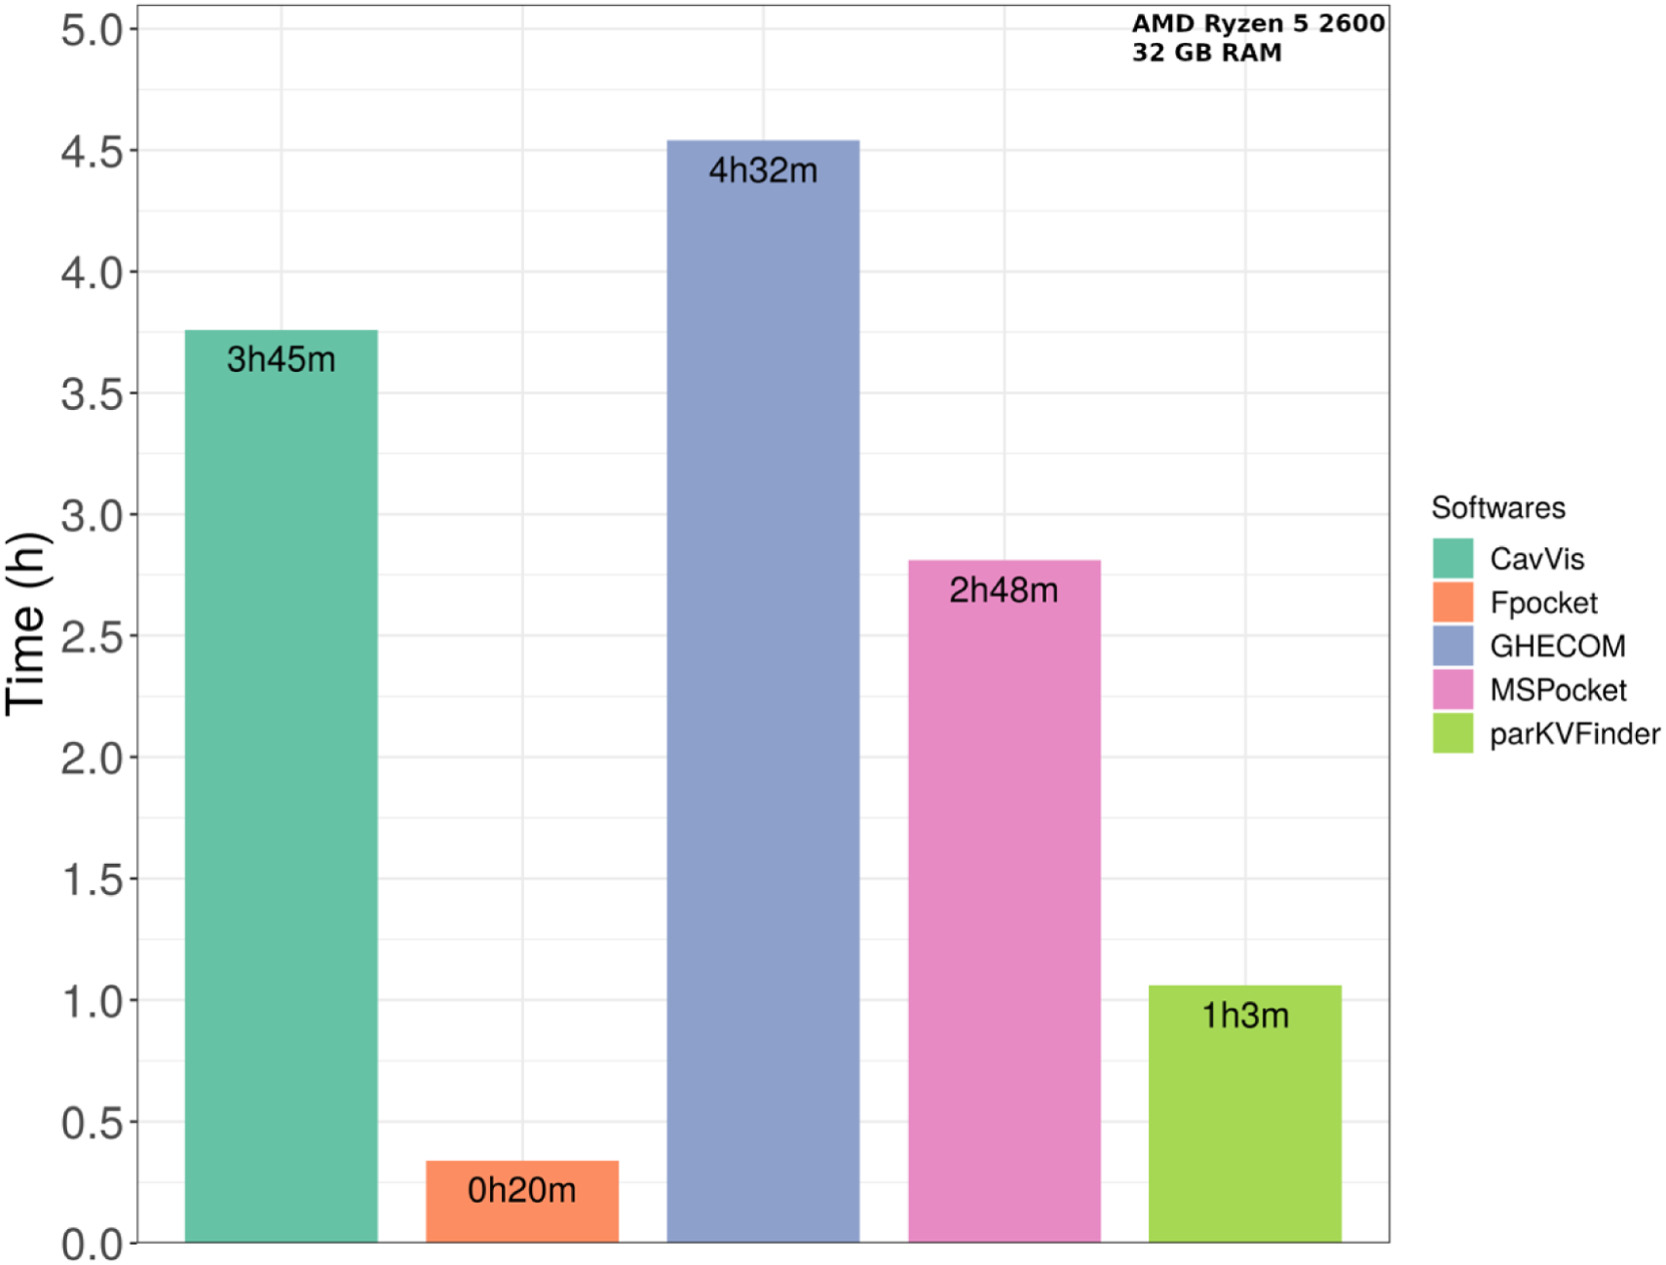
\includegraphics[scale=0.9]{images/hiv1-protease-dm-times.png}}
  \centerline{\tiny{\textbf{Source:} Reprinted from \cite{guerra2020}. Licensed under \href{https://creativecommons.org/licenses/by/4.0/}{CC BY 4.0}.}}
  \caption[Computational time of the benchmarking methods]{\textbf{Computational time of the benchmarking methods.}}
  \label{fig:hiv1-protease-dm-times}
\end{figure}

It is important to highlight that the details of the simulations and analyses are available in the article published in the \textit{SoftwareX} \cite{guerra2020}.

\subsubsection{Mayaro and Other Alphaviruses \label{sec:parkvfinder-mayaro}}

\ac{MAYV} is an emerging arbovirus prevalent in Central and South America, associated with a debilitating and arthritogenic disease. The ectodmains E1 and E2 are essential transmembrane alphaviral proteins that form heterodimers. These heterodimers, organized into trimers, compose the spikes on the viral surface, extending through the lipid bilayer and interacting with the nucleocapsid proteins C. These spikes play a crucial role in binding to cellular receptors, cell internalization, and membrane fusion. The subsquent release of \acs{MAYV} RNA into the cytoplasm triggers viral protein expression, replication, and the production of mature and infectious viral progeny. Given their central role, the E1 and E2 proteins of \acs{MAYV} are key targets for vaccine development and antiviral drugs \cite{ribeiro2021}. However, the lack of detailed structural information on these proteins has hindered the development of effective strategies to combat \acs{MAYV} infection.

The central region between the E1 and E2 proteins forms a cavity occupied by an extra-long density, not accounted for by side-chain residues (Figure \ref{fig:mayv-e1-e2}A and B). A similar density profile was previously observed in a cryo-electron map of the \ac{SINV}, suggesting a hydrophobic phospholipid tail (C18), termed a \textit{pocket factor}, might occupy this density and stabilize the hydrophobic pocket formed between E1 and E2 \cite{chen2018}. To gain a deeper understanding of the pocket environment and extract its chemical characteristics, we employed parKVFinder \cite{guerra2020} to comprehensively characterize the \acs{MAYV} pocket and compare it with pockets in other alphaviruses. The E1 and E2 ectodomains of \acs{MAYV} (PDB ID: 7KO8), \acs{SINV} (PDB ID: 6IMM), \ac{EEEV} (PDB ID: 6MX4), \ac{VEEV} (PDB ID: 3J0C), and \ac{CHIKV} (PDB ID: 6NK5) were used for the detection and characterization of the hydrophobic pocket. In \acs{MAYV}, the cavity between the E1 and E2 domains has a volume of $\sim$850 $\AA^3$ (Figure \ref{fig:mayv-e1-e2}D). This volume is quite similar across \acs{SINV}, \acs{EEEV}, and \acs{VEEV}, while in \acs{CHIKV}, the larger distance between E1 and E2 results in a larger volume.

\begin{figure}
  \centerline{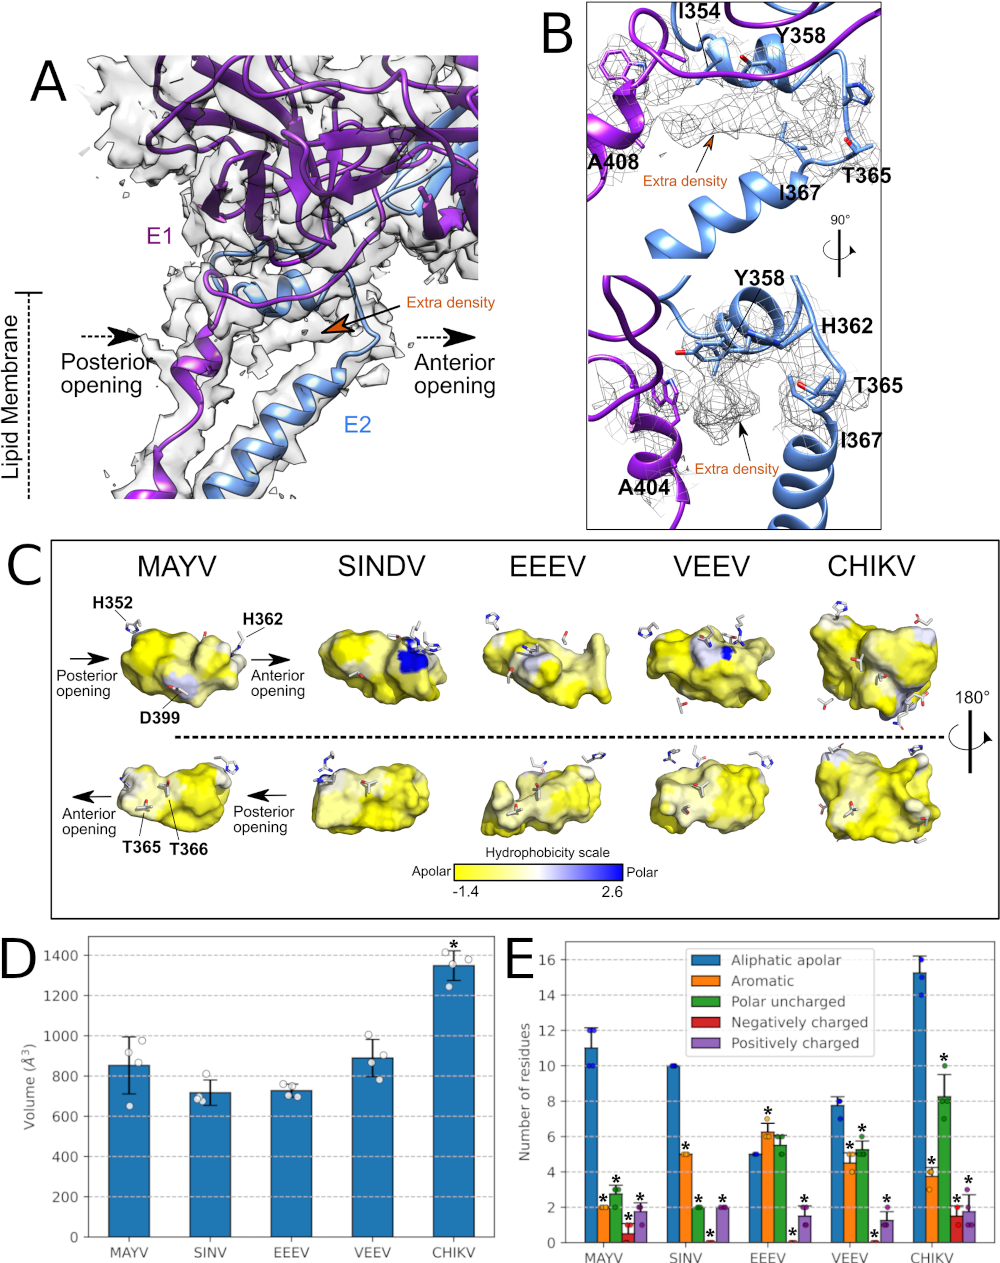
\includegraphics[scale=0.22]{images/mayv-e1-e2.png}}
  \centerline{\tiny{\textbf{Source:} Adapted from \cite{ribeiro2021}. Licensed under \href{https://creativecommons.org/licenses/by/4.0/}{CC BY 4.0}.}}
  \caption[MAYV E1 and E2 transmembrane domains and the hydrophobic cavity]{\textbf{MAYV E1 and E2 transmembrane domains and the hydrophobic cavity.} \textbf{(A)} \acs{3D} atomic model of \acs{MAYV} fitted to the density map, showing the upper portion of the E1 and E2 TM helices. The E1-E2 intersection forms a cavity with anterior and posterior openings. The observed extra density within the cavity is indicated. \textbf{(B)} Detail of the extra density found in the head region of E1-E2 and the surrounding residues. The density map of \acs{MAYV} is shown in mesh or surface representation. \textbf{(C)} Cavity detection in alphaviral structures. The cavity between the E1 and E2 domains is shown in surface representation and colored based on the Eisenberg & Weiss hydrophobicity scale, using the residues that form the cavity. Only polar residues are represented as sticks. \textbf{(D)} Cavity volume for the four E1-E2 heterodimers (n = 4 independent heterodimer structures) in the asymmetric unit. One-way ANOVA with Tukey's multiple comparison test was used to compare the \acs{MAYV} cavity volume with other alphaviruses (* indicates adj. p < 0.01 when compared to alphaviruses with \acs{MAYV}). \textbf{(E)} Number of residues in each of the four E1-E2 heterodimers (n = 4 independent heterodimer structures) in the asymmetric unit, separated by classes. One-way ANOVA with Tukey's multiple comparison test was used to compare the number of residues in the apolar aliphatic class with the other classes in the same alphavirus species (* indicates adj. p < 0.01 when comparing the apolar aliphatic class with the other classes). All data are presented as mean values +/- SD. Apolar aliphatic: ALA, VAL, ILE, LEU, GLY, PRO; Aromatic: PHE, TYR, TRP; Uncharged polar: SER, THR, CYS, MET, ASN, GLN; Negatively charged: GLU, ASP; Positively charged: ARG, LYS, HIS.}
  \label{fig:mayv-e1-e2}
\end{figure}

The hydrophobic nature of the alphavirus pocket is clearly observed by mapping the hydrophobicity surface (Figure \ref{fig:mayv-e1-e2}C) and the number of apolar residues forming the core of the cavity (Figure \ref{fig:mayv-e1-e2}E). The pocket density extends to polar residues, such as H362, T365, and T366 from the E2 domain at the posterior opening (Figure \ref{fig:mayv-e1-e2}C and E), indicating that the molecule may have an amphipathic nature, such as a fatty acid. Notably, T365 and T366 maintain a structurally conserved position in other alphaviruses or are replaced by serine, an even more polar residue. At the posterior opening, another histidine (H352 from E2) helps close the pocket, with histidine residues in similar positions observed in most alphaviruses, except SINV. Together, these findings indicate that alphaviruses have a consistent amphipathic cavity formed between the E1 and E2 domains in the outer membrane of the lipid bilayer. If the alphaviral pocket hosts a molecule, it would be chemically similar across different alphaviruses. The density map of \acs{MAYV} suggests that the extra density may be occupied by a fatty acid, potentially enhancing interactions between E1 and E2. Consequently, the pocket emerges as a potential target for the development of antiviral compounds against \acs{MAYV} and other alphaviruses through rational drug design.

On the other hand, alphavirus nucleocapsid proteins C are composed of two subdomains: a disordered N-terminal domain, responsible for binding to viral RNA (not observed in the \acs{MAYV} density map), and a structured C-terminal domain that non-covalently binds to E2 proteins (Figure \ref{fig:mayv-c-e2}). The N-terminal region has lower identity among alphaviruses and is reported as virus-specific \cite{ribeiro2021}. The \acs{MAYV} density map confirms the generally conserved structure of the C protein, forming two subdomains rich in beta sheets separated by a shallow cavity of $\sim$500 $\AA^3$ (Figure \ref{fig:mayv-c-e2}), wherein the C-terminal domain of the E2 protein non-covalently binds. The bottom of the pocket is hydrophobic, while its top has polar and charged residues. The interface between the capsid and the E2 protein involves the TPY consensus motif (residues T387, P398, and Y399; Figure \ref{fig:mayv-c-e2}), conserved within the \textit{Alphavirus} genus. Interestingly, small molecules proposed to inhibit the interaction between the capsid and the E2 protein contain heterocyclic rings, reinforcing the relevance of this type of contact for the capsid-E2 protein interaction and positioning this site as a potential drug target.

\begin{figure}[hp]
  \centerline{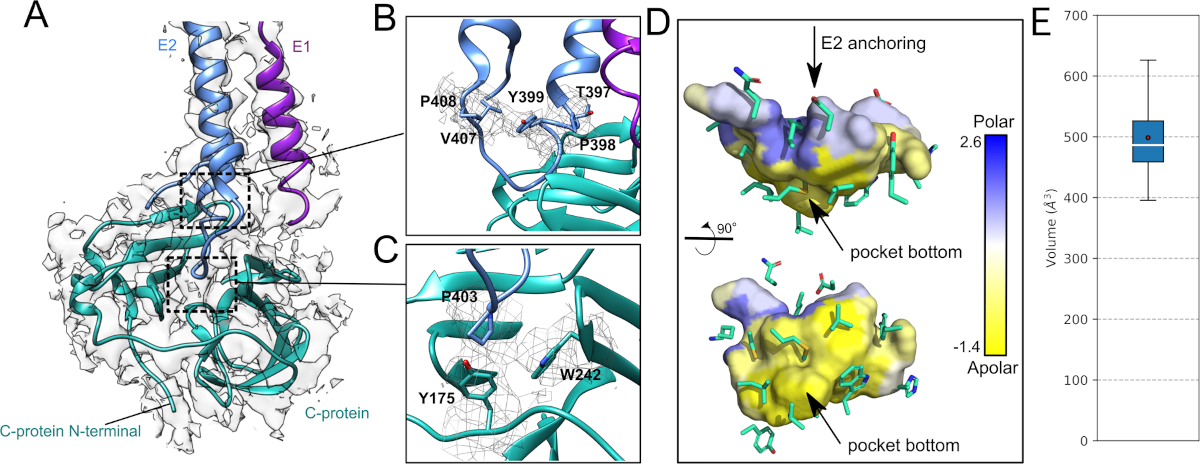
\includegraphics[scale=0.23]{images/mayv-c-e2.png}}
  \centerline{\tiny{\textbf{Source:} Adapted from \cite{ribeiro2021}. Licensed under \href{https://creativecommons.org/licenses/by/4.0/}{CC BY 4.0}.}}
  \caption[Interaction of MAYV capsid with the C-terminal domain of the E2 protein]{\textbf{Interaction of MAYV capsid with the C-terminal domain of the E2 protein.} \textbf{(A)} 3D atomic model of \acs{MAYV} fitted to the density map obtained by cryo-electron microscopy. The C, E1, and E2 proteins are represented as cyan, purple, and blue cartoons, respectively. \textbf{(B)} The interaction of the TPY motif (residues T387, P398, and Y399) with the C protein. \textbf{(C)} Residues P403 and T402 of E2 and their interaction with the aromatic residues Y175 and W242 in the C protein. The density map of \acs{MAYV} is shown in mesh representation. \textbf{(D)} Cavity detection in the C protein of \acs{MAYV}, showing a hydrophobic environment at the bottom of the pocket and a polar and charged environment at the outer edges of the cavity. The cavity in the C protein that binds to the C-terminal domain of E2 is shown in surface representation and colored according to the Eisenberg hydrophobic consensus scale. The C protein residues surrounding the cavity are represented as sticks. \textbf{(E)} Boxplot of the cavity volume for the four capsids (n = 4 independent capsid structures) in the asymmetric unit. In the boxplot, the box represents the interquartile range ($IQR$) ($67.5 \AA^3$), the 75th percentile ($Q3$) ($526.2 \AA^3$), and the 25th percentile ($Q1$) ($458.7 \AA^3$). The central line indicates the median ($486.3 \AA^3$), and the mean ($498.6 \AA^3$) is indicated by a dot. The "whiskers" with a minimum value ($395.7 \AA^3$) and a maximum value ($626.2 \AA^3$) are determined using $Q1-1.5 \cdot IQR$ and $Q3+1.5 \cdot IQR$, respectively.}
  \label{fig:mayv-c-e2}
\end{figure}

It is important to note that the complete results and details of the analyses are available in the article published in the \textit{Nature Communications} \cite{ribeiro2021}.

\subsection{Discussion}

parKVFinder emerges as a powerful tool for detecting and characterizing biomolecular cavities, offering enhanced capabilities through integration with PyMOL—a user-friendly platform for visualization. The routine optimization and parallelization have significantly improved its performance, surpassing its predecessor, KVFinder \cite{guerra2019,guerra2020}. In the case study involving the \acs{MD} of HIV-1 protease, parKVFinder demonstrated a remarkable capacity to accurately describe the conformational dynamics of the active site, outperforming other geometry-based methods both in accuracy and computational time. The investigation of the hydrophobic pocket within alphaviruses, particularly in MAYV, not only identifies on potential drug targets but also highlights shared structural features across alphaviruses. This consistency in the nature of the cavity underscores parKVFinder's utility in uncovering fundamental aspects of biomolecular structures.

Despite the successful application of parKVFinder in \acs{MD} simulations \cite{guerra2020} and a comparative study \cite{ribeiro2021}, certain limitations became apparent in automated tasks and systematic binding site comparisons. Consequently, there arises a need for a more suitable tool tailored to data science applications, providing straightforward access to functions and data structures for efficient analysis. Nevertheless, it is important to acknowledge that parKVFinder still plays a significant role within KVFinder suite. Its contribution lies notably in optimizing detection and characterization parameters through the PyMOL graphical plugin (PyMOL2 parKVFinder Tools), leveraging its visual cues. These fine-tuned parameters seamlessly integrate into automated studies and systematic binding site comparisons. In essence, parKVFinder continues to be indispensable for conducting structural and functional analyses focused on individual biomolecular structures.

\section{pyKVFinder}

In data science, data-intensive cavity analysis requires efficient routines and algorithms built on easily manipulable data structures. Cavities identified by parKVFinder, like those in other well-known programs such as fpocket \cite{fpocket}, GHECOM \cite{ghecom}, and POVME 3.0 \cite{povme}, are human-readable and easily displayed in molecular visualization programs. However, they lack suitable structuring for direct integration into automated protocols and data science applications. Addressing this need, we developed the \ac{pyKVFinder} \cite{guerra2021}, an open-source Python package, licensed under GPL v3.0, for detecting and characterizing cavities in biomolecular structures within automated protocols and data science applications. Subsequently, pyKVFinder was published in \textit{BMC Bioinformatics} \cite{guerra2021} and released as pyKVFinder \href{https://github.com/LBC-LNBio/pyKVFinder/releases/tag/v0.2.5}{v0.2.5}, with the current version being \href{https://github.com/LBC-LNBio/pyKVFinder/releases/tag/v0.6.9}{v0.6.9}. The source code is under continuous development and available at the following repository: https://github.com/LBC-LNBio/pyKVFinder.

pyKVFinder employs a \ac{SWIG} (\url{https://www.swig.org}) to extend \acs{3D} grid operations, written in C, to the high-level programming language, Python. by doing so, pyKVFinder can be imported as a package in the Python environment and users can decide to run the full cavity detection and characterization workflow through the \textit{pyKVFinder.run\_workflow} function or run pyKVFinder functions in a stepwise fashion (Figure \ref{fig:code-workflow}). For further details on the functions of pyKVFinder package, please refer to the article published in \textit{BMC Bioinformatics} \cite{guerra2021} or the documentation page at \url{https://lbc-lnbio.github.io/pyKVFinder/}.

\begin{figure}[h]
  \centering
  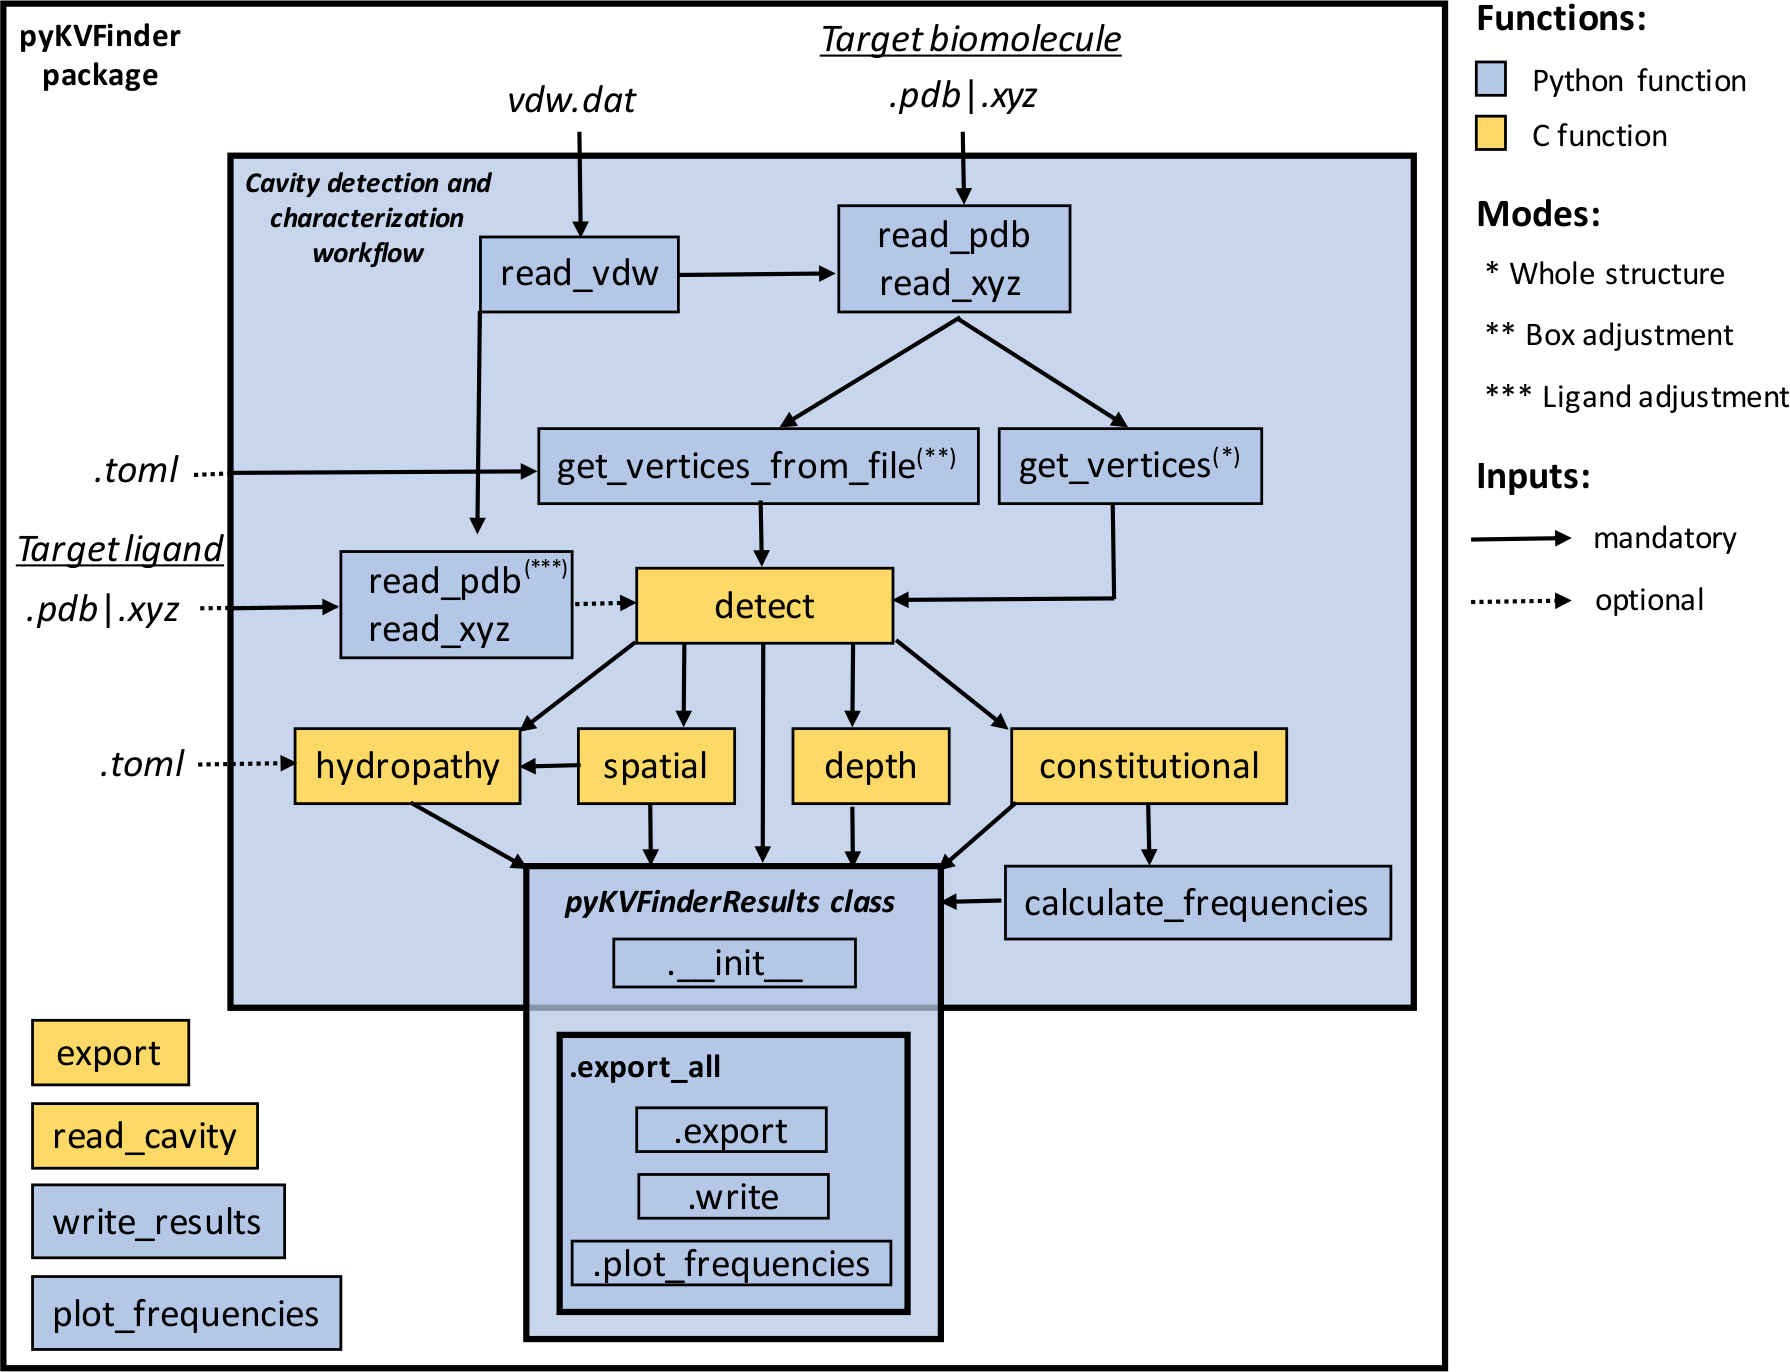
\includegraphics[scale=0.7]{images/code-workflow.png}
  \centerline{\tiny{\textbf{Source:} Reprinted from \cite{guerra2021}. Licensed under \href{https://creativecommons.org/licenses/by/4.0/}{CC BY 4.0}.}}
  \caption[Diagram of cavity detection and characterization workflow using pyKVFinder package]{\textbf{Diagram of cavity detection and characterization workflow using pyKVFinder package.}  The flowchart illustrates function calls and their dependencies for performing cavity detection and characterization with pyKVFinder package}
  \label{fig:code-workflow}
\end{figure}

In pyKVFinder, the target biomolecule is inserted in a regular 3D grid, stored as an \ac{ndarray} from the NumPy package \cite{numpy}. To detect cavities, pyKVFinder uses a dual-probe algorithm, as shown in Figure \ref{fig:parkvfinder-schema}, which scans the biomolecular structure for regions of inaccessibility (\ie, cavities). In addition to cavity properties like volume, area, and interface residues stored as Python dictionaries, pyKVFinder calculates cavity depth and hydrophobicity. Both cavity points and these morphological and physicochemical properties are stored in \acsp{ndarray} and can be visualized using Python molecular visualization packages (\eg, NGLView \cite{nglview} and plotly \cite{plotly}). Moreover, pyKVFinder can be integrated with various scientific packages and libraries (\eg, scikit-learn \cite{scikit-learn} and SciPy \cite{scipy}) for mathematical calculations, statistical analysis, and \acs{3D} visualization using interactive interfaces (\eg, IPython, Jupyter, and JupyterLab notebooks). Thus, pyKVFinder facilitates complex analyses of biostructural data with protocols and algorithms within the Python ecosystem, serving as a building block for new applications in data science, rational drug design, and drug discovery. In essence, pyKVFinder provides a versatile means of detecting and characterizing biomolecular cavities and integrating this information into automated protocols and data science applications.

The computational performance of pyKVFinder was also assessed on kv1000 \cite{guerra2020}, presenting a considerably shorter runtime compared to parKVFinder, averaging 31\% faster (Figure \ref{fig:pykvfinder-speedup}). The primary reason for this performance gain lies in the additional possibility to parallelize routines, \ie, atom insertion into the 3D grid in the detection function (\ie, \textit{pyKVFinder.detect}), based on \acsp{ndarray}. The most significant improvement was observed in proteins with over 2000 atoms, achieving a speedup of $\sim$4.3 times in proteins with 11000 atoms, benefiting the growing number of currently resolved high-order structures. For very small proteins ($\less 2000$ atoms), which represent a smaller portion of available structures, pyKVFinder's performance gain was not significant or even lower than that of parKVFinder, mainly due to the Python reading of the target's PDB or XYZ file. 

\begin{figure}[h]
  \centering
  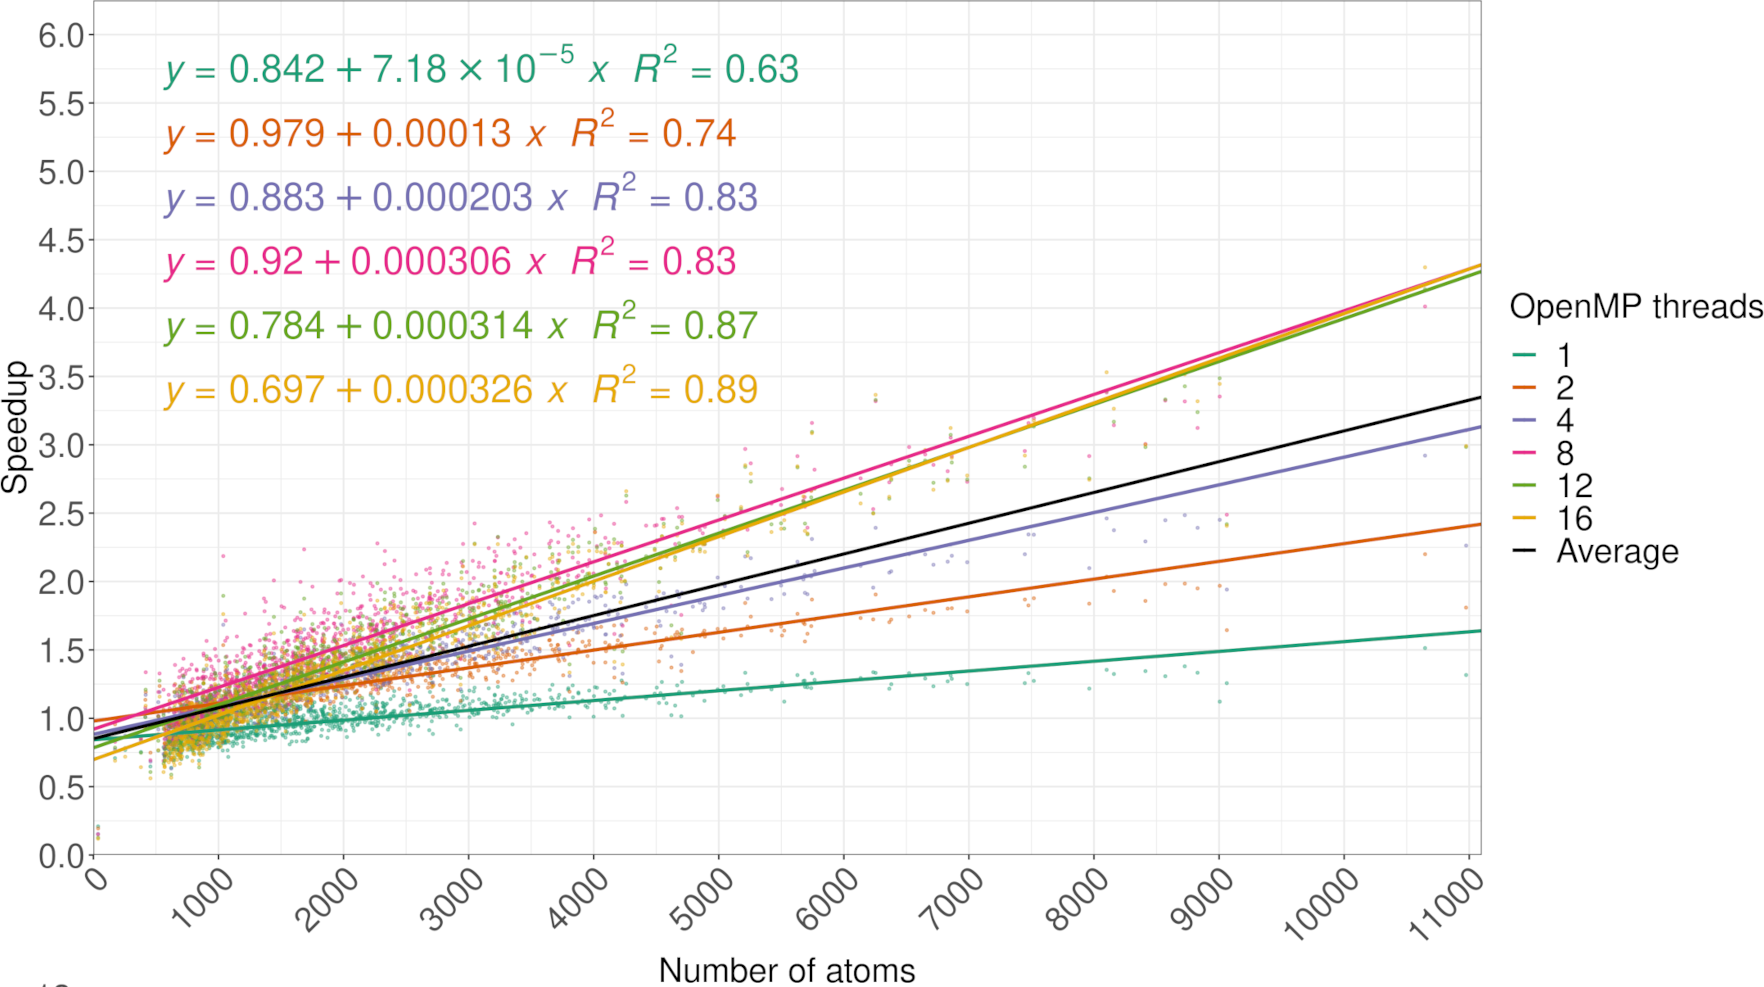
\includegraphics[scale=1]{images/pykvfinder-speedup.png}
  \caption[Speedup of pyKVFinder compared to parKVFinder]{\textbf{Speedup of pyKVFinder compared to parKVFinder.} The speedup is the ratio of pyKVFinder's execution time to parKVFinder's execution time, applying the same number of OpenMP threads, for different numbers of atoms.}
  \label{fig:pykvfinder-speedup}
\end{figure}

Even with the addition of new characterizations such as depth and hydrophobicity, pyKVFinder's performance was only reduced by an average of 5\% (for depth) and 4\% (for hydrophobicity), regardless of the number of threads used (Figure \ref{fig:pykvfinder-parkvfinder-kv1000-comparison}). Additionally, the scalability of pyKVFinder with an increasing number of threads, as well as the absolute time to perform cavity detection, is presented in Figure \ref{fig:pykvfinder-parkvfinder-kv1000-comparison}, following the behavior exhibited by parKVFinder \cite{guerra2020}.

\begin{figure}[h]
  \centering
  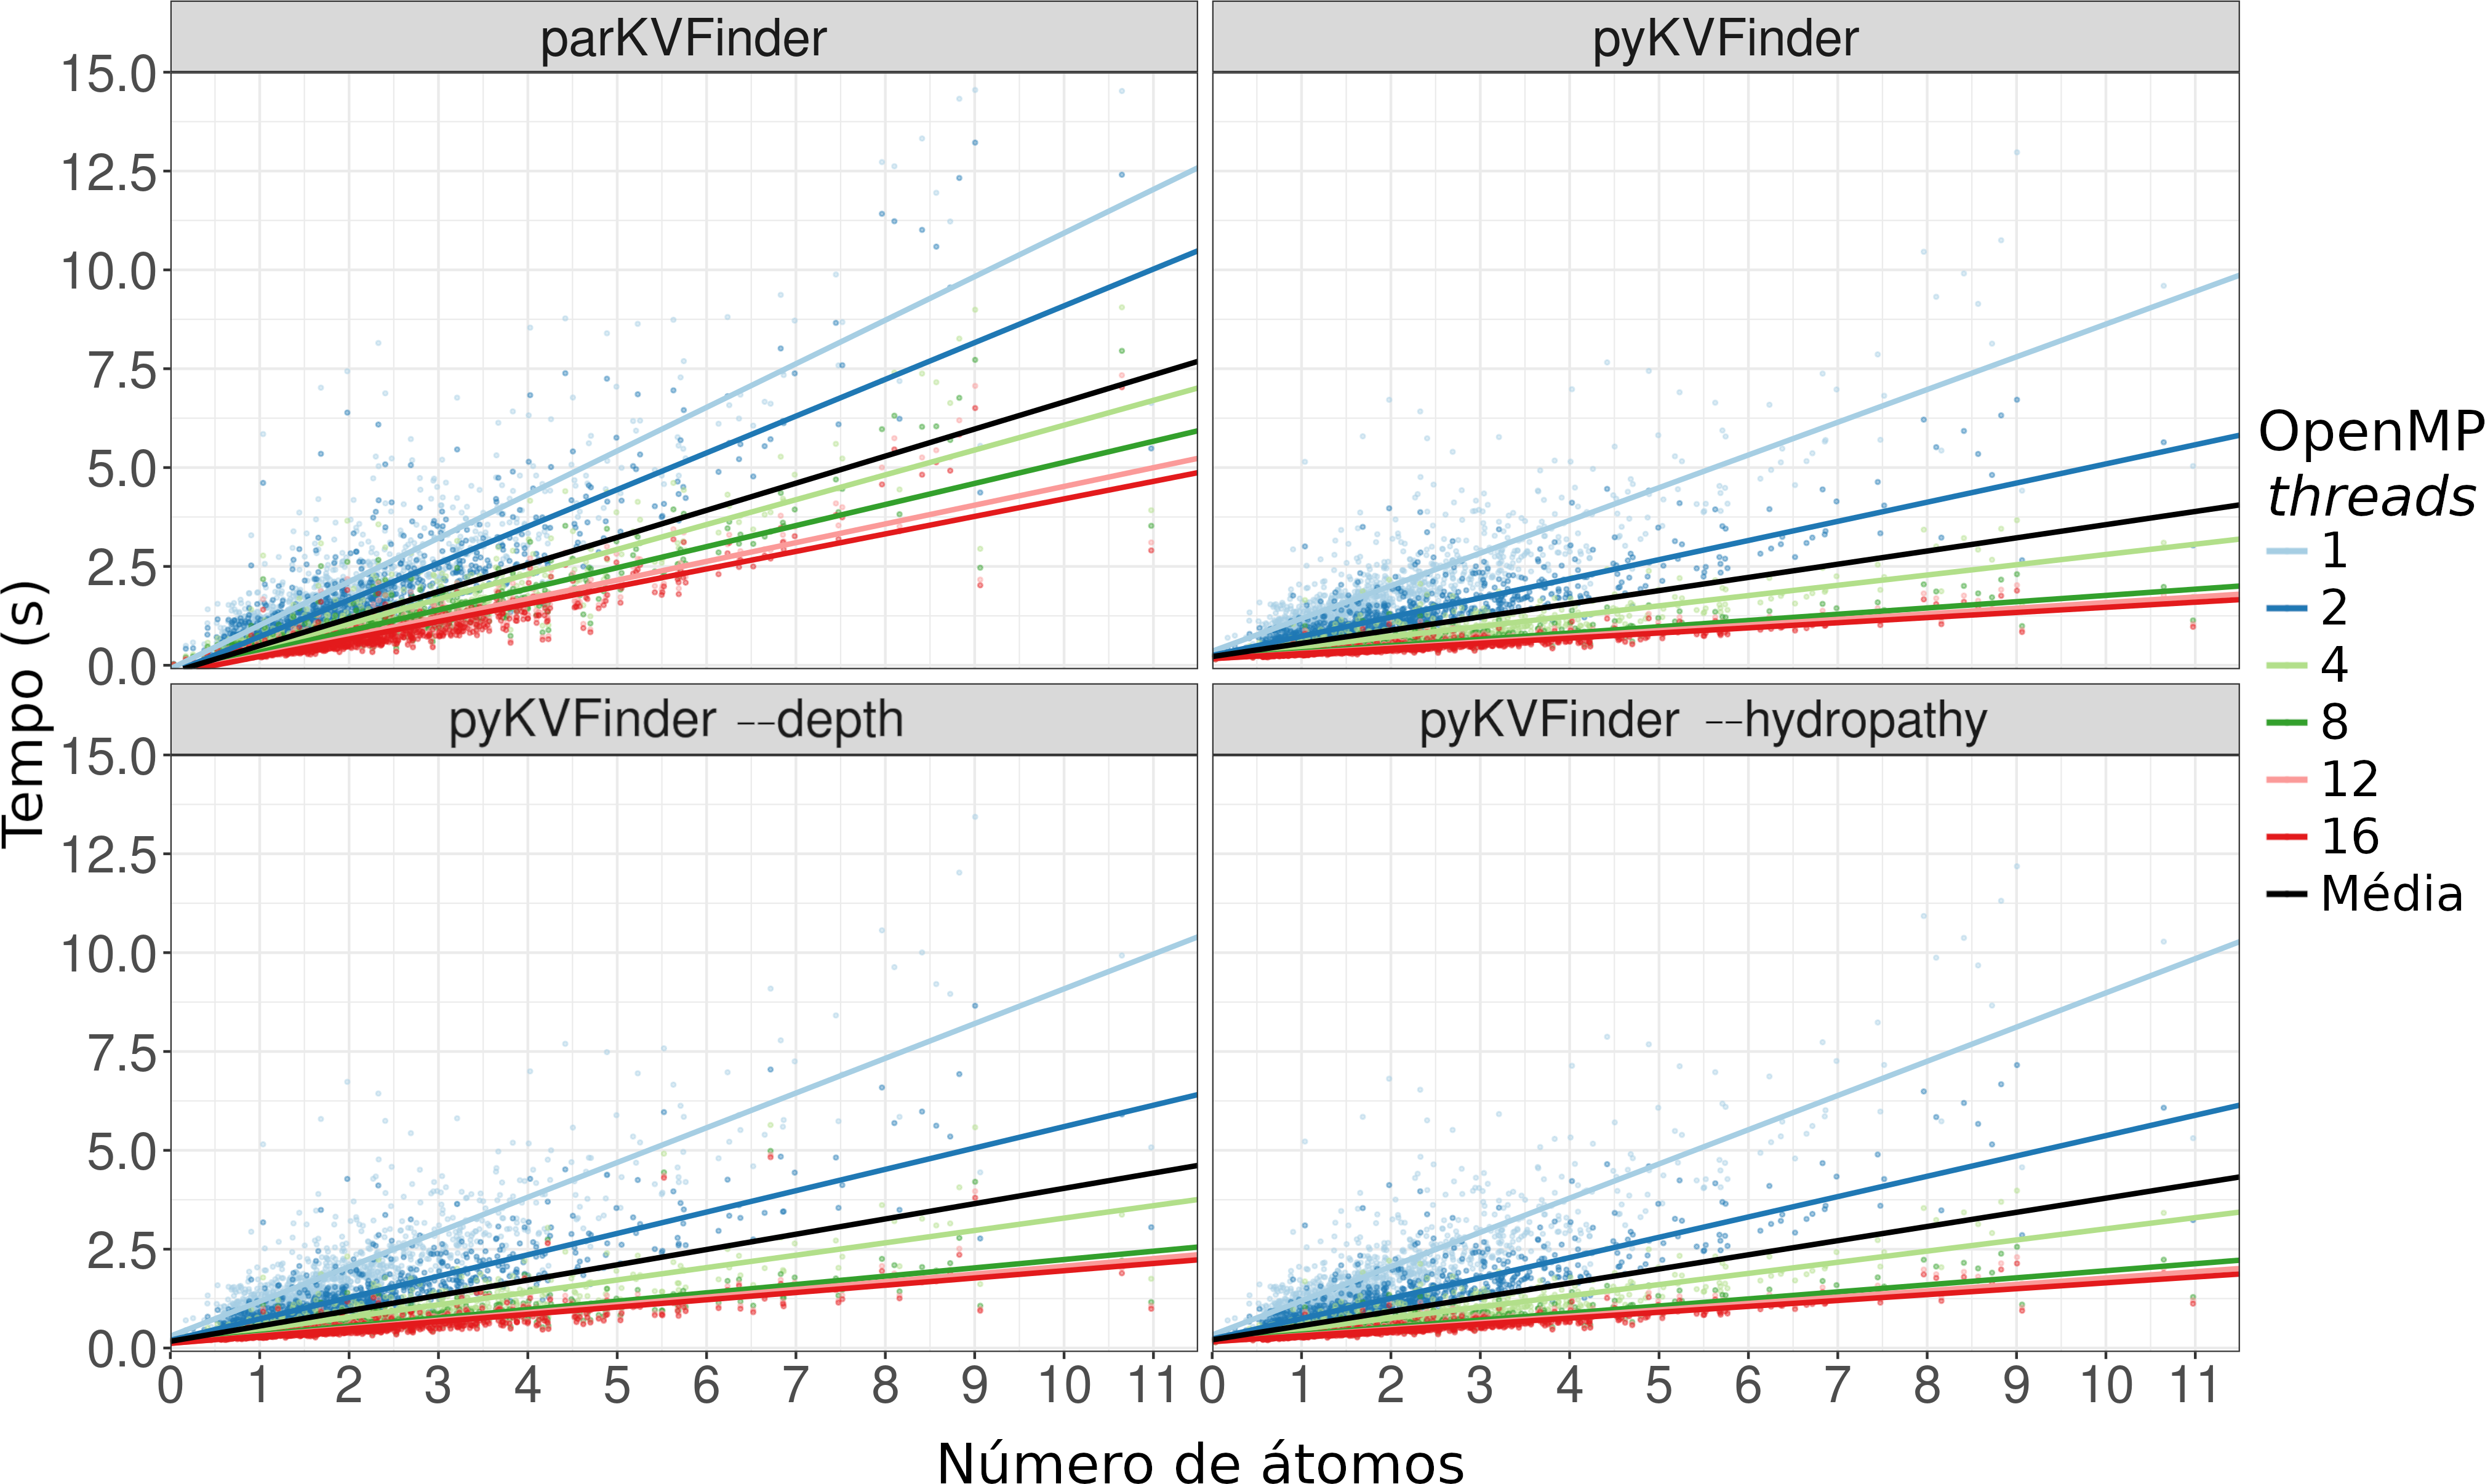
\includegraphics[scale=1]{images/pykvfinder-parkvfinder-kv1000-comparison.png}
  \caption[Computational time as a function of the number of atoms with different numbers of threads for parKVFinder and pyKVFinder]{\textbf{Computational time as a function of the number of atoms with different numbers of threads for parKVFinder and pyKVFinder.} Top left panel: parKVFinder. Top right panel: pyKVFinder with default characterization (volume, area, and interface residues). Bottom left panel: pyKVFinder with default and depth characterizations. Bottom right panel: pyKVFinder with default and hydrophobicity characterizations.}
  \label{fig:pykvfinder-parkvfinder-kv1000-comparison}
\end{figure}

Therefore, experienced users requiring scripting routines are encouraged to use pyKVFinder due to its enhanced performance, while newcomers should prioritize parKVFinder due to its monolithic behavior and ease of installation and execution. 

\subsection{Implementations of New Characterizations}

Within the context of pyKVFinder, in collaboration with Dr. György Szalóki (Laboratoire Hétérochimie Fondamentale et Appliquée - Université Toulouse III Paul Sabatier - France), the scope of the KVFinder suite has been expanded to a new class of molecules called supramolecular cages. These cages are interconnected molecules that come together through non-covalent interactions, forming an internal cavity capable of encapsulating molecules or ions. The shape and size of the cavity are important parameters that can be easily determined by geometric algorithms, aiding in the rational design of supramolecular cages. In this context, new characterizations applicable to both cage and biomolecular contexts have been developed.

\subsubsection{Molecular Volume Estimation \label{sec:molecular-volume-estimation}}

The \textit{pyKVFinder.Molecule} class, introduced in pyKVFinder \href{https://github.com/LBC-LNBio/pyKVFinder/releases/tag/v0.5.0}{v0.5.0}, enables users to model detailed molecular surfaces, following mathematical formulations shown in Figure \ref{fig:surface-representation}, within the pyKVFinder framework. In this approach, molecules are inserted into a regular 3D grid, taking into account the \acs{vdW} radii of each of the atoms in the molecule. Users can customize these radii through a configuration file (\textit{\href{https://github.com/LBC-LNBio/pyKVFinder/blob/master/pyKVFinder/data/vdw.dat}{vdw.dat}}), as well as the surface representation, \ie \acs{vdW} surface, \acs{SES} and \acs{SAS}. Conveniently, users can represent the \acs{vdW} surface by invoking \textit{Molecule.vdw}, \acs{SES} by invoking \textit{Molecule.surface('SES')}, and \acs{SAS} by invoking \textit{Molecule.surface('SAS')} (Figure \ref{fig:molecular-modeling}). Within the 3D grid, each voxel is assigned as a molecule ($0$) or solvent ($1$) point, allowing the estimation of the \acs{vdW} volume by summing the voxels labeled as a molecule through the \textit{Molecule.volume} method. The comprehensive implementation of these features for molecular modeling and characterization has been described and applied in an article published in the \textit{Journal of Chemical Information and Modeling} \cite{guerra2023B}.

\begin{figure}[h]
  \centering
  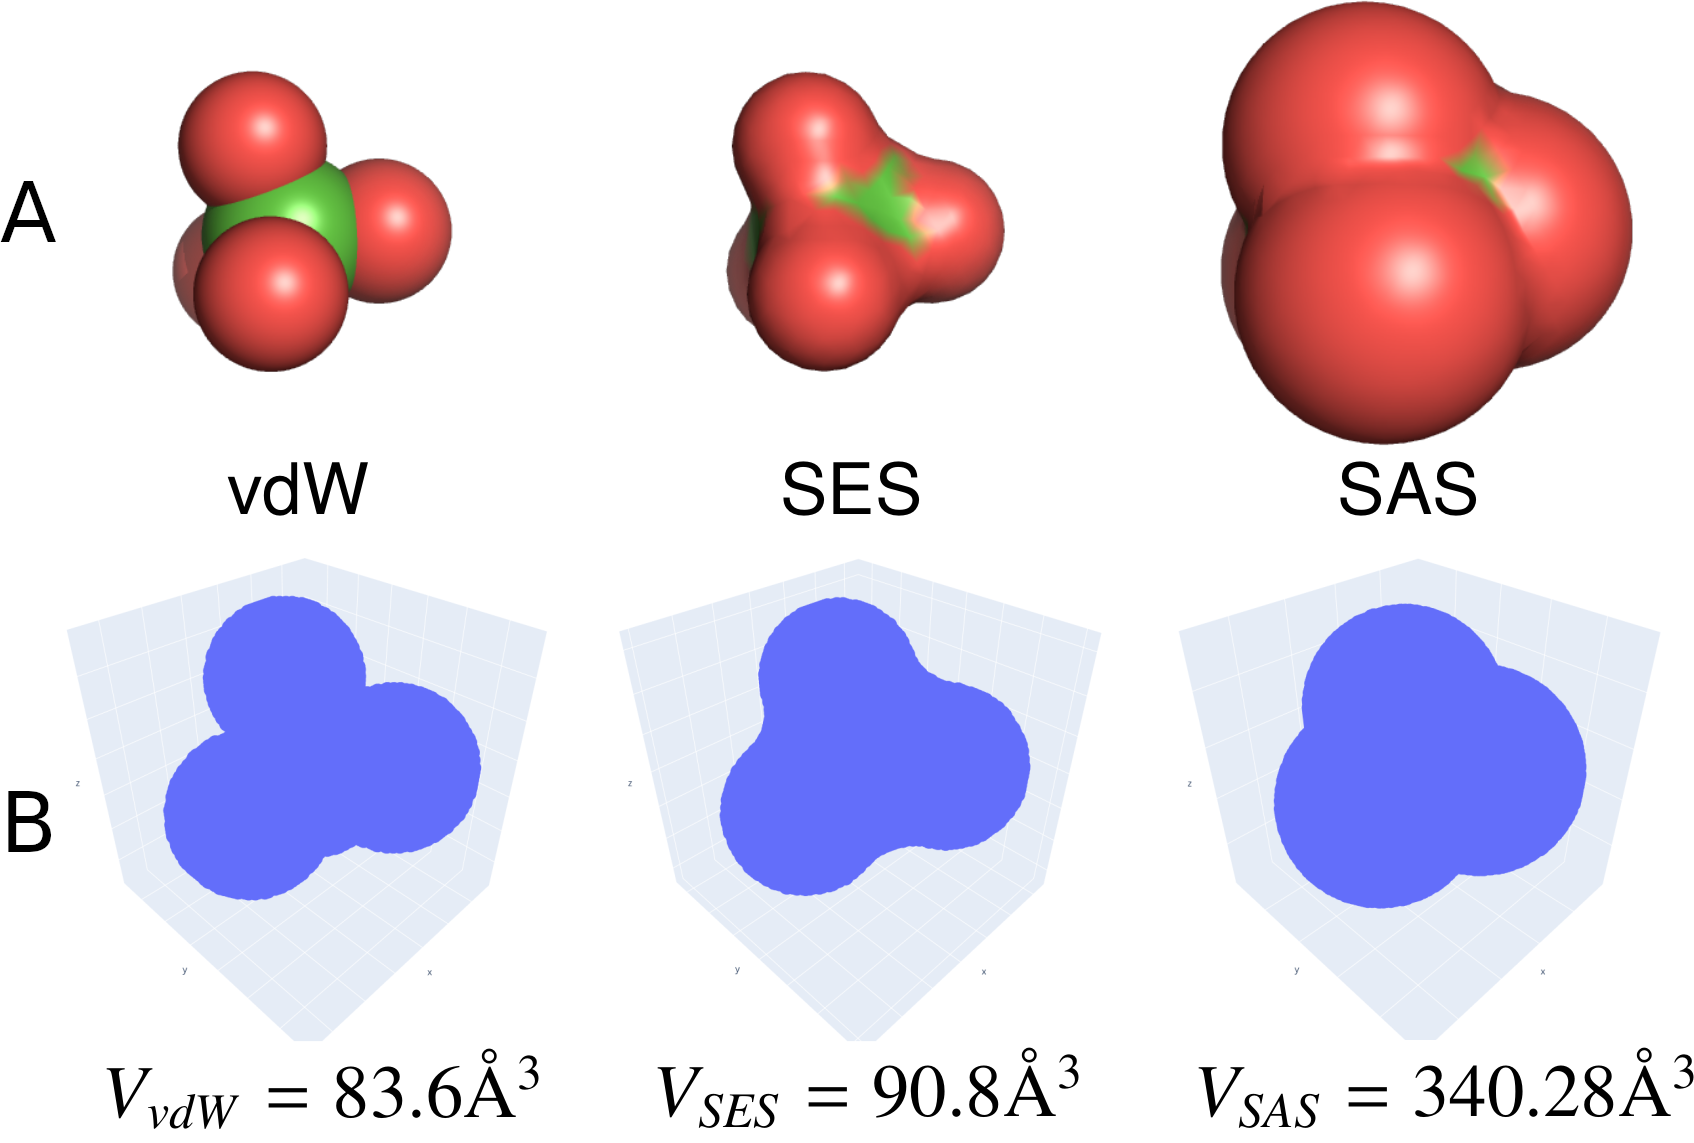
\includegraphics[scale=1.5]{images/molecular-modeling.png}
  \caption[Molecular modeling and volume estimation of perchlorate ($ClO_4$)]{\textbf{Molecular modeling and volume estimation of perchlorate ($ClO_4$).} \textbf{(A)} Molecular surface of \acs{vdW} (left panel), \acs{SES} (center panel), and \acs{SAS} (right panel) in the PyMOL molecular viewer. \textbf{(B)} Modeling and estimation of the \acs{vdW} (left panel), \acs{SES} (center panel), and \acs{SAS} (right panel) molecular volume by pyKVFinder.}
  \label{fig:molecular-modeling}
\end{figure}

\subsubsection{Opening Characterization}

Understanding the characteristics of supramolecular cages, such as volume (Figure \ref{fig:cage-characterization}A) and openings (Figure \ref{fig:cage-characterization}B), which drive the encapsulation of reactive intermediates, is crucial for the rational design of new supramolecular cages with enhanced catalytic properties. In this regard, we have developed an opening characterization using pyKVFinder, allowing the identification of openings, determination of the area of these openings, and the largest spherical probe (\ie, atom) that can pass through each opening, as shown in Figure \ref{fig:cage-characterization}.

\begin{figure}[ht]
  \centering
  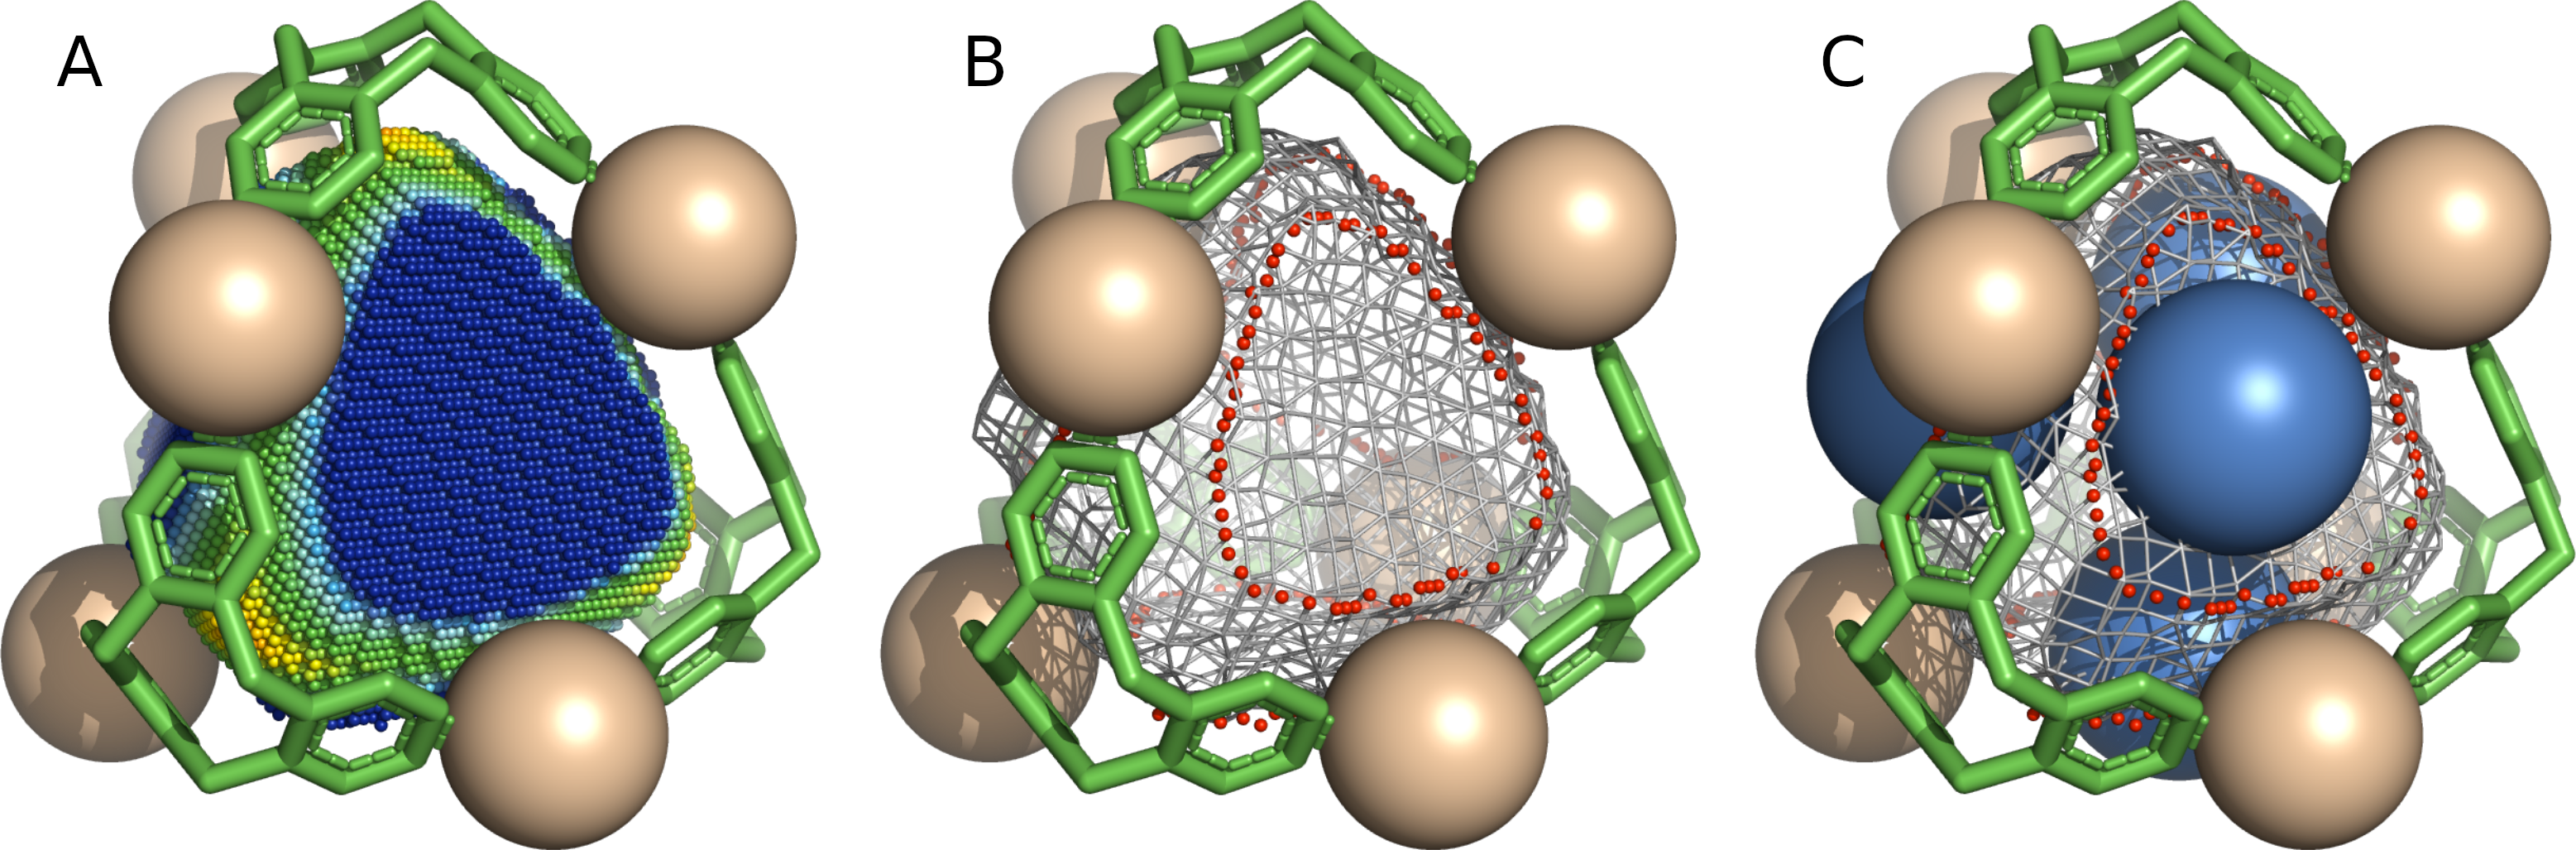
\includegraphics[scale=1.2]{images/cage-characterization.png}
  \caption[Supramolecular cage characterizations]{\textbf{Supramolecular cage characterizations.} \textbf{(A)} Volume and depth. Points are colored according to depth, with blue for shallower and red for deeper points. \textbf{(B)} Openings (red points) and opening area. \textbf{(C)} Largest spherical probe (blue sphere) accessible to the cage cavity.}
  \label{fig:cage-characterization}
\end{figure}

The dual-probe system uses integer identifiers for cavity points ($1$), biomolecule points ($0$), and solvent points ($-1$). After cavity segmentation, performed by the \ac{DFS} algorithm, the cavity points are marked with values $\geq2$, and the cavity points that did not reach the volume cutoff are retained with the value $1$. From this voxel classification, cavity points ($\geq2$) located at a grid unit from a solvent point ($-1$), following the structuring element's rank 3 and connectivity 1 relationship (Figure \ref{fig:structuring-elements}), are identified as cavity-solvent boundary points, marked with the negative value of the corresponding cavity's numeric identifier, as described for depth characterization \cite{guerra2019,guerra2021}. From these boundary points, the surface area is calculated using the area estimation methodology of the KVFinder suite \cite{guerra2019,guerra2020}, which corresponds to the opening area. Subsequently, the cavity-solvent boundary points located at a grid unit from a biomolecule point ($0$), following the structuring element's rank 3 and connectivity 1 relationship (Figure \ref{fig:structuring-elements}), are identified as opening points. At this stage, a new \acs{3D} grid is generated to accumulate the opening points, which are marked with the value $1$, while the remaining points receive the value $0$. Afterwards, the \acs{DFS} algorithm is repourpouse to segment boundary points, to identify distinct openings, where opening points are marked with values $\geq2$ (Figure \ref{fig:cage-characterization}B), and openings with fewer points than a cutoff defined by the user are kept with the value $1$. Finally, for each identified opening, the midpoint is calculated, and the largest sphere centered in this midpoint is fitted inside the respective boundary, defining the largest atom that can pass through this opening (Figure \ref{fig:cage-characterization}C).

\begin{figure}[h]
  \centering
  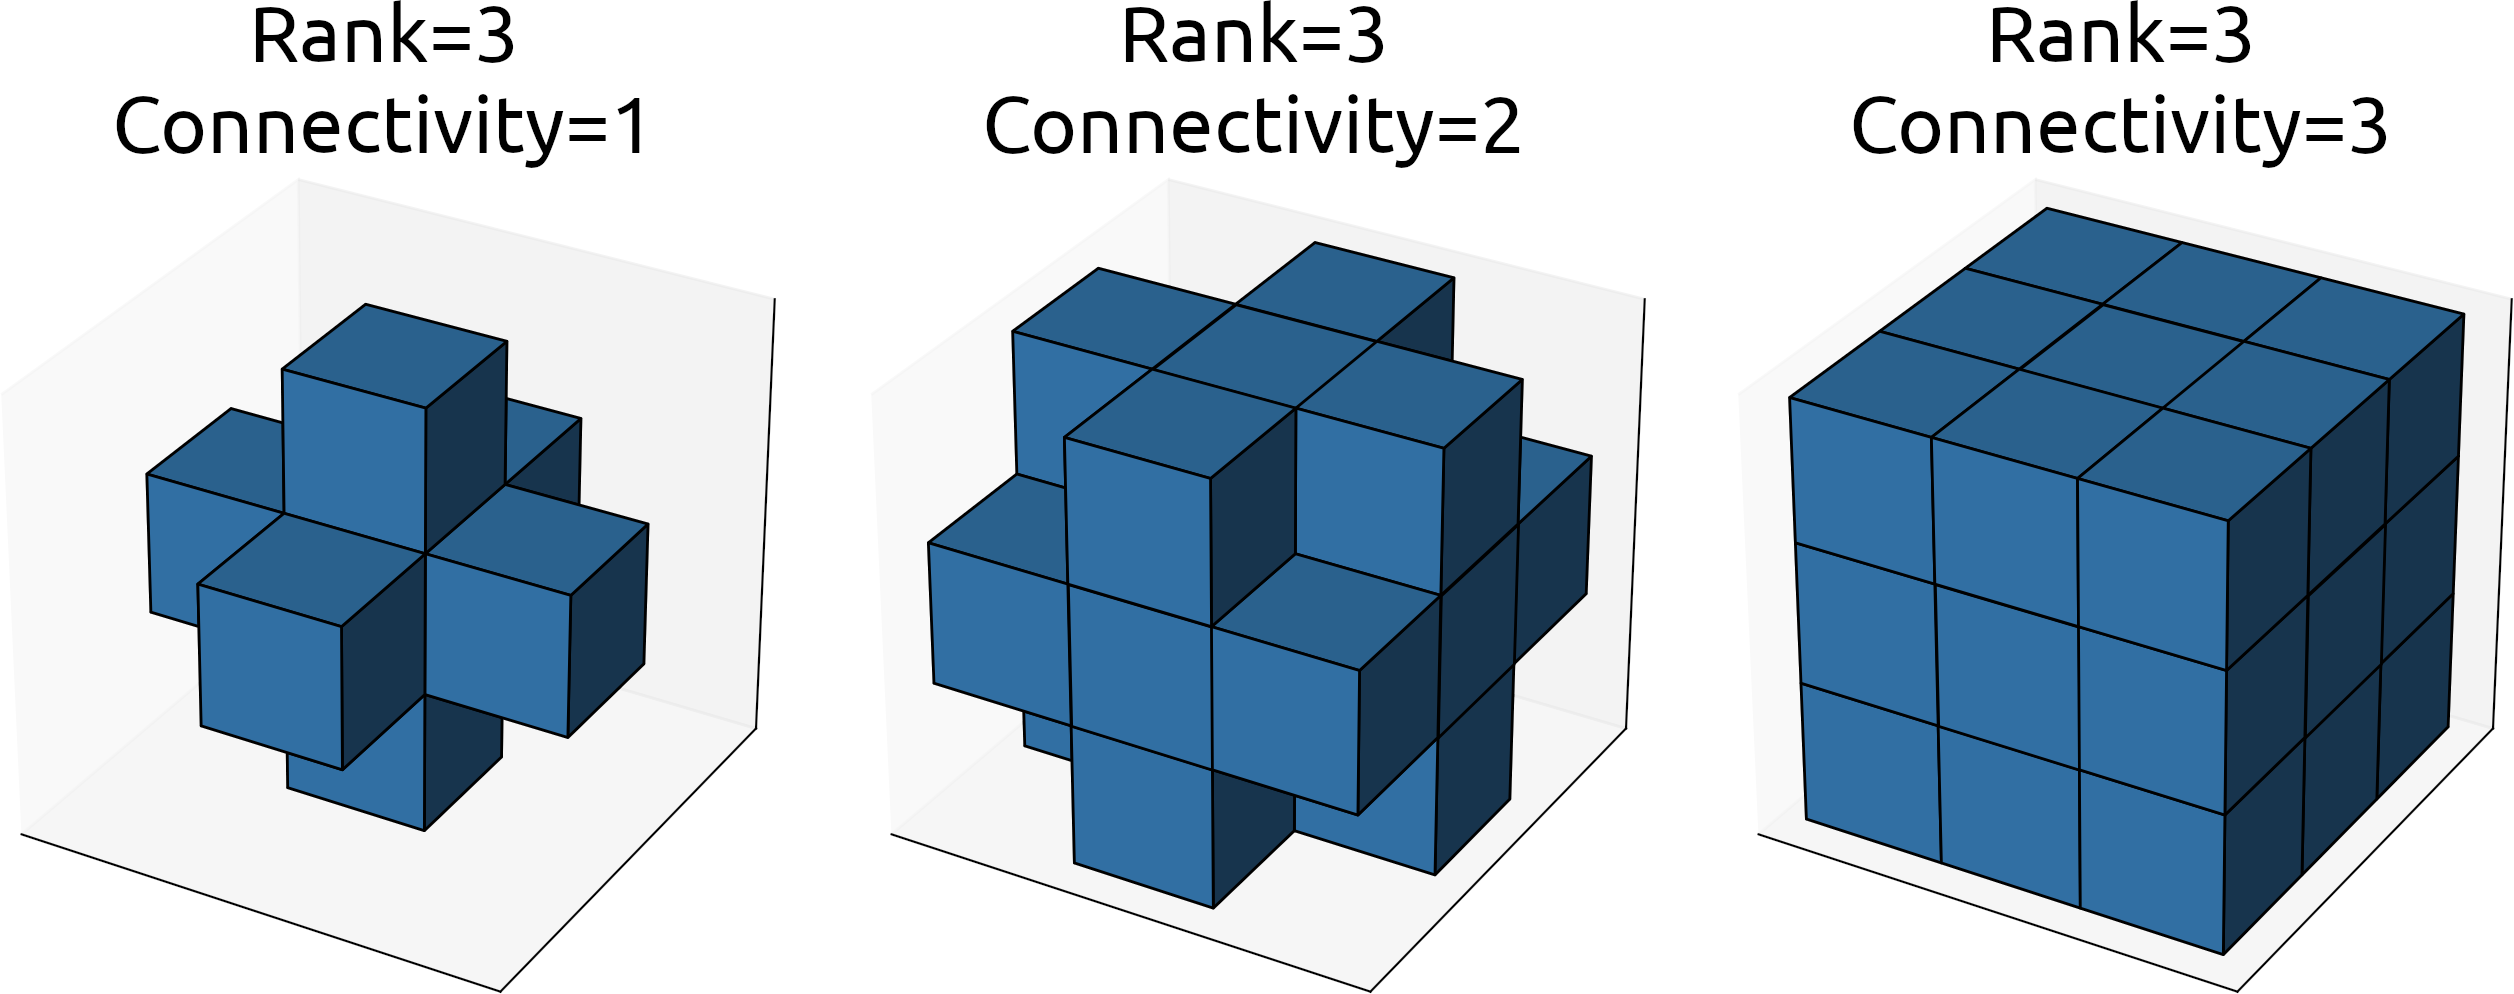
\includegraphics[scale=0.6]{images/3D-binary-structure.png}
  \caption[Structuring elements for spatial filters]{\textbf{Structuring elements for spatial filters.}}
  \label{fig:structuring-elements}
\end{figure}

\subsection{Case Studies}

The pyKVFinder was applied in two case studies published in scientific journals to investigate proteins of therapeutic interest. These analyses explored the characteristics of cavities in proteins homologous to the \ac{ADRP} domain of \ac{SARS-CoV-2} and the \acs{MD} of the \acs{ADRP} domain of \acs{SARS-CoV-2} \cite{guerra2021}. Next, we will describe each of these case studies in detail.

\subsubsection{SARS-CoV-2 and Homologous Proteins \label{sec:pykvfinder-sars-cov-2}}

Among the 15 \ac{Nsps} of the \acs{SARS-CoV-2}, the \acs{ADRP} domain of nsp3 protein, also known as the macrodomain, is noteworthy \cite{michalska2020}. This domain has been under investigation to comprehend its exact functions in the coronavirus life cycle, as the \acs{ADRP} domain recognizes ADP-ribose 1'-phosphate and appears to play a crucial role in virulence and innate immunity regulation against infection \cite{fehr2016,claverie2020}. Recent efforts have aimed to characterize the ADP-ribose substrate-binding site and evaluate this site as a potential target for antiviral drugs.

\begin{figure}[h]
  \centering
  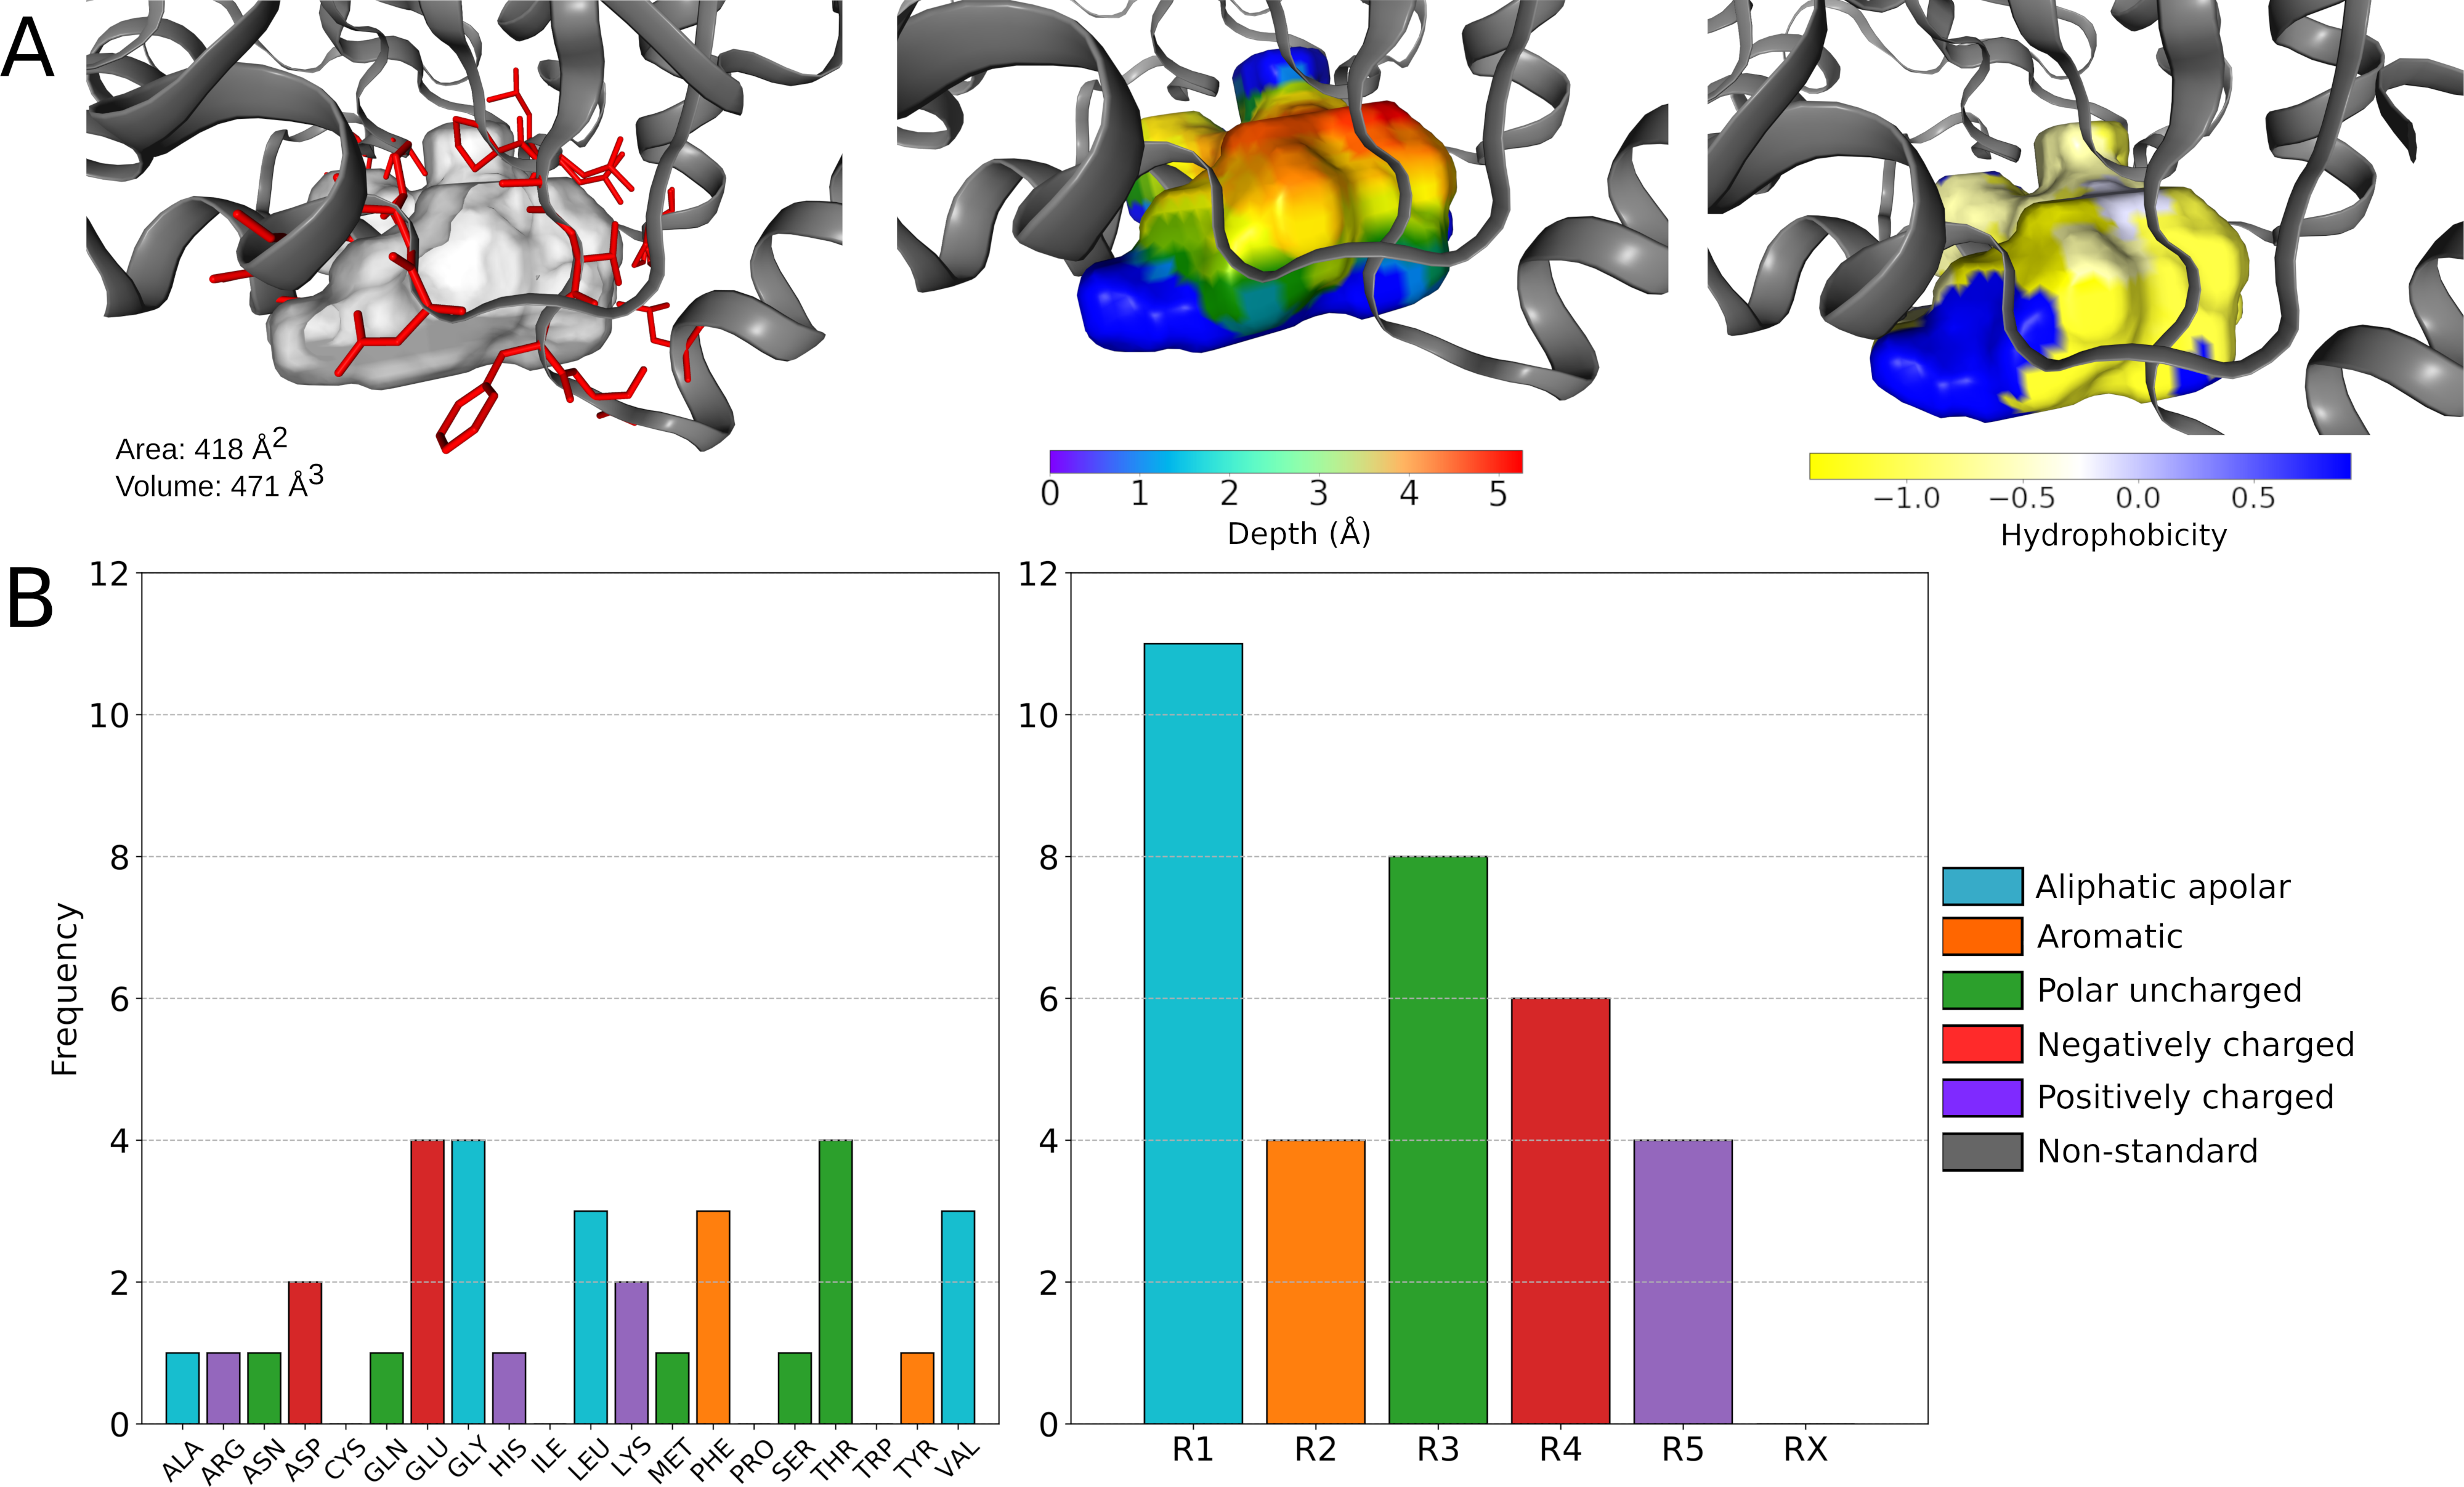
\includegraphics[scale=0.9]{images/adrp-sars-cov-2-analysis.png}
  \centerline{\tiny{\textbf{Source:} Adapted from \cite{guerra2021}. Licensed under \href{https://creativecommons.org/licenses/by/4.0/}{CC BY 4.0}.}}
  \caption[Characterization of the ADRP substrate-binding cavity of SARS-CoV-2]{\textbf{Characterization of the ADRP substrate-binding cavity of SARS-CoV-2.} \textbf{(A)} Characterizations of the substrate-binding site of the ADRP domain of SARS-CoV-2 (PDB ID: 6WEN). Left panel: Detected cavity represented as a gray surface and the surrounding residues as red sticks. The cavity area and volume are shown. Center panel: Cavity colored by depth. Right panel: Cavity colored by hydrophobicity using the Eisenberg and Weiss scale. \textbf{(B)} Bar chart of interface residue frequencies. Left panel: Amino acids. Right panel: Classes of amino acids.}
  \label{fig:binding-site-analysis}
\end{figure}

In this context, we employed pyKVFinder to detect and characterize a cavity present in the \acs{ADRP} protein of \acs{SARS-CoV-2}, corresponding to the substrate-binding site (Figure \ref{fig:binding-site-analysis}A). After cavity detection, we characterized its volume, area, and the interface residues involved in the cavity (Figure \ref{fig:binding-site-analysis}A, left panel). It noteworthy that 3D visualization of the protein and cavity can be performed in the Jupyter notebook itself using the NGLView package \cite{nglview}. However, users have the freedom to choose other molecular visualization tools (\eg, PyMOL \cite{pymol}, ChimeraX \cite{chimerax}, NGL Viewer \cite{nglviewer}, or VMD \cite{vmd}). Additionally, we inspected the substrate-binding cavity of ADRP in terms of depth (Figure \ref{fig:binding-site-analysis}A, center panel) and hydrophobicity (Figure \ref{fig:binding-site-analysis}A, right panel). These descriptions are relevant for drug development \cite{brosey2021}. Despite being solvent-exposed in the apo form, the cavity has internal components (in red) that reach a more central portion of the ADRP beta-sheet (Figure \ref{fig:binding-site-analysis}A, center panel). Hydrophobicity analysis shows that the cavity's core is more hydrophobic (in yellow), with some polar residues at the edges (in blue), contributing to the rational design of more specific ligands.

As illustrated in Figure \ref{fig:binding-site-analysis}A, the ADP-ribose binding site forms a cleft between the \textalpha-helices of the \acs{ADRP} domain, and key contacts involve residues from loop regions, explaining the flexibility of the pocket during substrate binding \cite{michalska2020}. We then determined the composition of the residues forming the cavity and presented their frequencies in a histogram (Figure \ref{fig:binding-site-analysis}B), using the matplotlib library \cite{matplotlib}. However, users are free to analyze the data and present results using their preferred graphical library.

\begin{figure}[h]
  \centering
  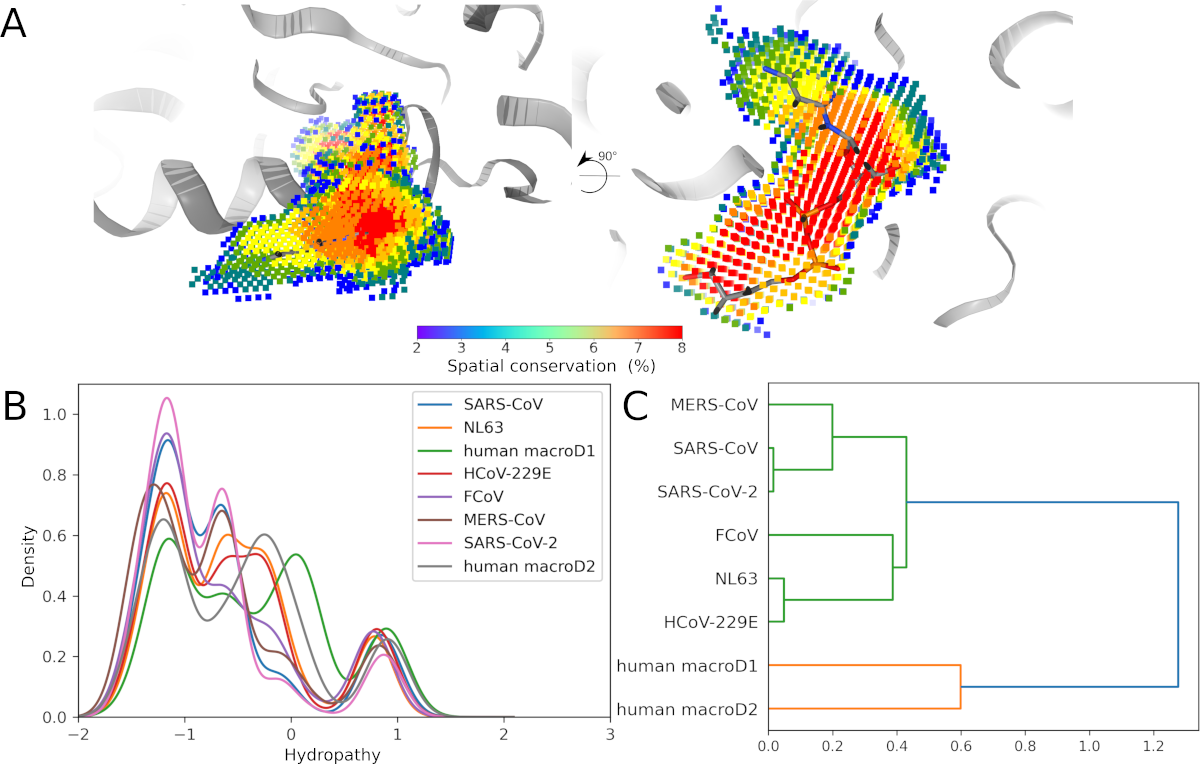
\includegraphics[scale=0.9]{images/adrp-sars-cov-2-conservation-analysis.png}
  \centerline{\tiny{\textbf{Source:} Adapted from \cite{guerra2021}. Licensed under \href{https://creativecommons.org/licenses/by/4.0/}{CC BY 4.0}.}}
  \caption[Comparative study of the ADRP substrate-binding site of SARS-CoV-2 and related proteins]{\textbf{Comparative study of the ADRP substrate-binding site of SARS-CoV-2 and related proteins.} \textbf{(A)} Conservation analysis of the ADP-ribose binding site in the ADRP domain of SARS-CoV-2 (PDB ID: 6WEN, chain A), SARS-CoV (PDB ID: 2ACF, chain B), MERS-CoV (PDB ID: 5HIH, chain A), NL63 (PDB ID: 2VRI, chain A), HCoV-229E (PDB ID: 3EJG, chain A), FCoV (PDB ID: 3ETI, chain B), and human macrodomain proteins macroD1 (PDB ID: 2X47, chain A) and macroD2 (PDB ID: 6Y73, chain D). The cavity points detected in at least two structures are colored by conservation percentage. \textbf{(B)} Hydropathy profile. \textbf{(C)} Hierarchical clustering dendrogram of residue frequency. Pearson correlation metric was used to assess similarity, and complete linkage method was chosen as the linking method. All graphics and images were generated in a Jupyter notebook. Three-dimensional structure images were created using the NGLView package \cite{nglview}, while graphics were built using the matplotlib package \cite{matplotlib}.}
  \label{fig:conservation-analysis}
\end{figure}

To compare the composition of this ADRP binding cavity with that of other related proteins, we conducted the same analysis on seven other selected proteins based on structural homology and alignment using Dali \cite{dali}. The proteins related to the ADRP domain of SARS-CoV-2 (PDB ID: 6WEN, chain A) are: MERS-CoV (PDB ID: 5HIH, chain A), NL63 (PDB ID: 2VRI, chain A), HCoV-229E (PDB ID: 3EJG, chain A), FCoV (PDB ID: 3ETI, chain B), and human macrodomain proteins macroD1 (PDB ID: 2X47, chain A) and macroD2 (PDB ID: 6Y73, chain D). Structures in the apo form were realigned using the MUSTANG algorithm \cite{mustang} of the YASARA program \cite{yasara}. By applying arithmetic operations on the matrices of the detected cavities, we determined the conservation of the cavity across species. As observed in Figure \ref{fig:conservation-analysis}A, the core of the ADRP cavity (red points) is highly conserved among the analyzed species, being occupied by the ADP's diphosphate and ribose, as well as the second ribose linked to ADP in the substrate-bound form of ADRP. On the other hand, adenosine occupies a less conserved region of the cavity (blue points), indicating that the structure of this site undergoes changes in some species to accommodate the ADP-ribose substrate.

To compare the hydrophobicity of the cavity across species, we plotted a hydrophobicity distribution using the matplotlib library \cite{matplotlib}, as shown in Figure \ref{fig:conservation-analysis}B. The distribution clearly reveals the hydrophobic nature of the pocket, widely shared among the ADRP substrate-binding cavities of coronaviruses. Interestingly, human proteins macroD1 and macroD2 seem to exhibit a less pronounced hydrophobicity distribution.

With pyKVFinder, we can calculate the frequency of residues composing the cavity. Using the SciPy library \cite{scipy}, we performed hierarchical clustering of these frequencies and presented the dendrogram in Figure \ref{fig:conservation-analysis}C. In this dendrogram, we observe that the cavity of SARS-CoV-2 ADRP clusters with that of SARS-CoV, demonstrating high similarity between these betacoronaviruses. Next to them, we can observe another betacoronavirus, MERS-CoV. In turn, alphacoronaviruses NL63 and HCoV-229E, and feline FCoV cluster together. Further away from the coronavirus macrodomain domains are the two human macrodomain proteins, macroD1 and D2. Despite the ADRP or macroD1/D2 cavities sharing the same substrate, ADP-ribose, these results indicate that the residue profile around these cavities follows evolutionary traces.

To demonstrate the functionalities and advantages of pyKVFinder, we conducted this study in a Jupyter notebook, executing step-by-step pyKVFinder functions. The notebook with the complete case study is available at \url{https://github.com/LBC-LNBio/pyKVFinder/blob/master/examples/conservation-analysis/conservation-analysis.ipynb}. A detailed description of this analysis is provided in the article published in the \textit{BMC Bioinformatics} \cite{guerra2021}.

\subsubsection{Molecular Dynamics of the ADRP Domain of SARS-CoV-2}

In this context, the computational performance of pyKVFinder was evaluated in \acs{MD} simulations of the ADRP domain of SARS-CoV-2 (PDB ID: 6W02, chain B) without its ligand, ADP-ribose, for a period of 600 ns, with frame extraction every 1 ns. This analysis was repeated with other well-known tools: parKVFinder v1.1.3 \cite{guerra2020}, POVME 3.0 \cite{povme}, fpocket \cite{fpocket}, GHECOM \cite{ghecom}, MSPocket \cite{mspocket}, and Biobb\_vs \cite{biobbvs}. All these methods successfully detected the substrate-binding site of the ADRP, where the shape and volume varied slightly during the MD simulation (Figure \ref{fig:pykvfinder-benchmarking}). The shapes of the cavities detected by pyKVFinder and parKVFinder precisely fit the original ligand in the binding site, similar to MSPocket (Figure \ref{fig:pykvfinder-benchmarking}A). Additionally, the volume calculated by pyKVFinder ($346.8 \pm 78.7 \AA^3$) and parKVFinder ($346.5 \pm 79.3 \AA^3$) closely relates to the volume of ADP-ribose ($351.1 \AA^3$; molecular surface volume estimated by the YASARA program), which originally occupied the substrate-binding site in the crystallographic structure used in the MD simulations (Figure \ref{fig:pykvfinder-benchmarking}B).

\begin{figure}[h]
  \centering
  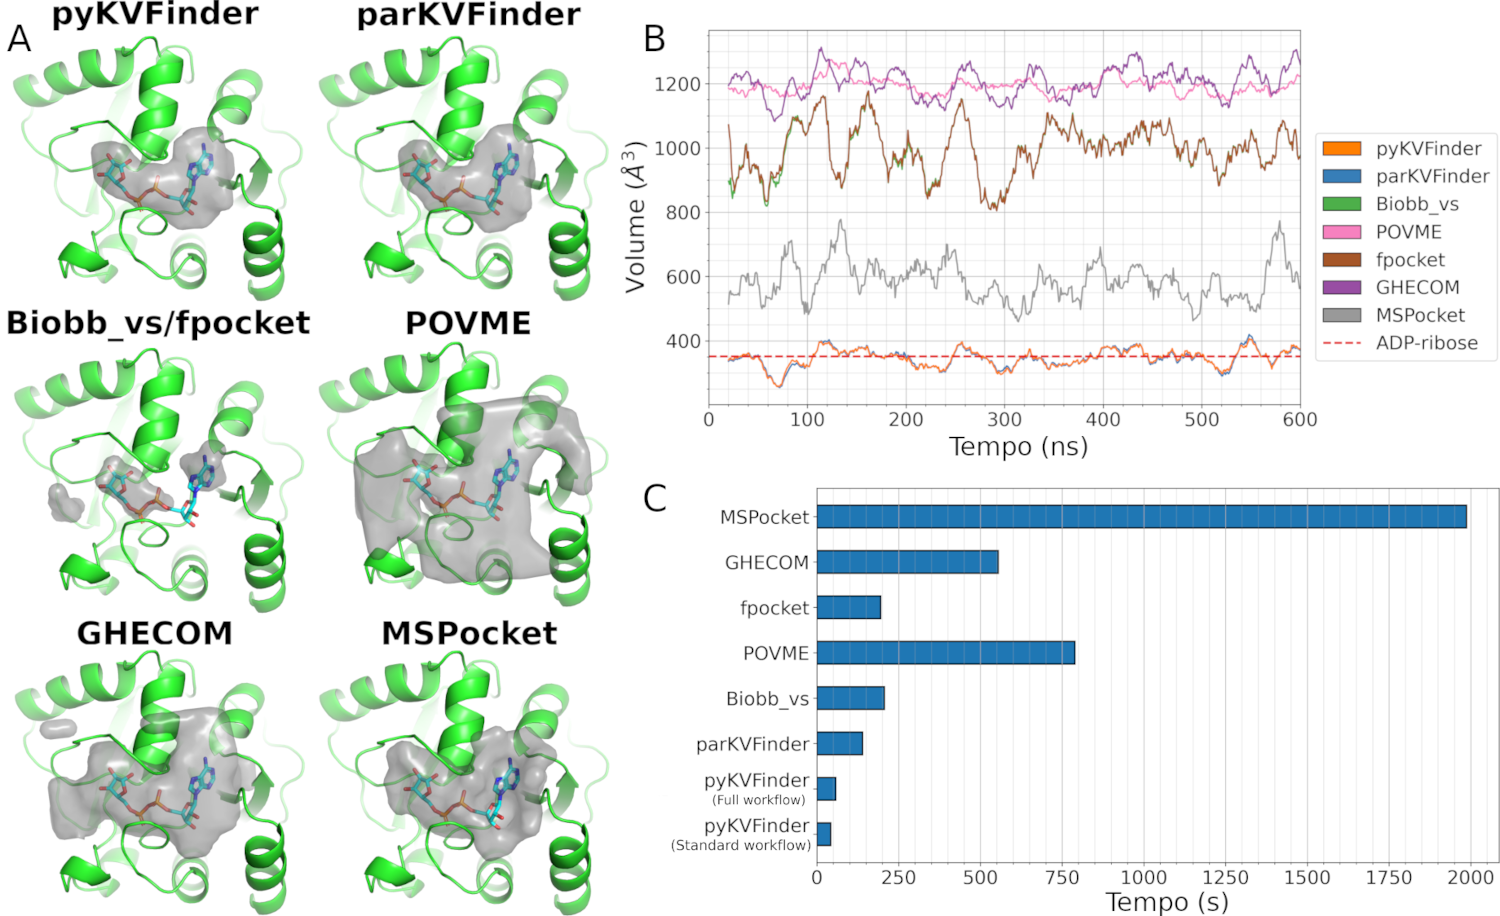
\includegraphics[scale=1]{images/pykvfinder-benchmarking.png}
  \centerline{\tiny{\textbf{Source:} Reprinted from \cite{guerra2021}. Licensed under \href{https://creativecommons.org/licenses/by/4.0/}{CC BY 4.0}.}}
  \caption[Performance evaluation of benchmarking methods for the ADRP substrate-binding site detection]{\textbf{Performance evaluation of benchmarking methods for the ADRP substrate-binding site detection.} \textbf{(A)} Protein structures (shown in green cartoons) in frame 30 (with the lowest RMSD compared to the crystallographic structure) of the ADRP domain trajectory with corresponding detected cavities (gray surfaces) by each benchmarking method. \textbf{(B)} Total volume of cavities detected at the substrate-binding site of ADRP over a 600 ns simulation. The total volume is calculated in a window of 20 frames. The red dashed line indicates the molecular surface volume of the ADP-ribose molecule, which originally occupied the substrate-binding site of ADRP in the crystallographic structure (PDB ID: 6W02, chain B). \textbf{(C)} Elapsed time to detect and characterize the substrate-binding site of ADRP. The default protocol of pyKVFinder, as well as parKVFinder, detects cavities and applies morphological (\eg, volume, area, and shape) and constitutional (e.g., interface residues and their frequencies) characterizations. The complete pyKVFinder protocol includes the default protocol with depth and hydrophobicity characterizations.}
  \label{fig:pykvfinder-benchmarking}
\end{figure}

In addition to accurately detecting biomolecular cavities, current tools must also perform perform fast cavity detection and characterizations. Therefore, we also assessed the elapsed time to execute these benchmarking methods (Figure \ref{fig:pykvfinder-benchmarking}C). pyKVFinder outperformed all analyzed methods in this aspect, even when applying the new characterization features of depth and hydrophobicity; the elapsed time of pyKVFinder increased only by 36\%, still outperforming other benchmarking methods. Furthermore, compared to parKVFinder, pyKVFinder was 3.3 times faster in detecting the ADRP binding site. The main reason for the performance gain is the additional possibility of parallelizing routines, \ie, atom insertion into the 3D grid in the detection function, based on ndarrays. Additionally, pyKVFinder's scalability, with an increase in the number of threads, follows the same behavior as parKVFinder \cite{guerra2020}. Therefore, pyKVFinder offers a more flexible and efficient option for experienced users requiring large-scale applications, while parKVFinder is more suitable for beginners due to its simplicity of installation and use.

To demonstrate the functionalities and advantages of pyKVFinder, we conducted this study in a Jupyter notebook, executing step-by-step pyKVFinder functions. The notebook with the complete case study is available at \url{https://github.com/LBC-LNBio/pyKVFinder/blob/master/examples/md-analysis/md-analysis.ipynb}. A detailed description of this analysis is provided in the article published in the \textit{BMC Bioinformatics} \cite{guerra2021}.

\subsection{Discussion}

Despite each method having its own set of characterizations to be performed on the detected cavities, the cavity data structure is only accessible within the Python ecosystem in pyKVFinder, which provides \acp{ndarray} and dictionaries in Python. By providing an accessible and flexible data structure, pyKVFinder allows users to develop new cavity characterizations, as well as analysis protocols based on these data structures. For example, in a recent study conducted by \cite{jefferson2023}, the cross-sectional area of cavities in related proteins was explored using pyKVFinder. This study demonstrated how the data structures provided by pyKVFinder can be used to delve deeper into cavity exploration and discover information relevant to drug development and understanding molecular interactions. Furthermore, the integration of pyKVFinder with the Python ecosystem expands the possibilities for data analysis and visualization, leveraging the robust scientific libraries available in Python language. This integration facilitates the implementation of advanced and customized analyses, enabling researchers to comprehensively explore the properties of biomolecular cavities and gain valuable insights.

In this way, pyKVFinder not only contributes to advancing research in drug discovery and rational drug design but also strengthens collaboration and knowledge sharing in the scientific community. By providing an accessible, flexible tool integrated into the Python ecosystem, pyKVFinder empowers researchers to explore biomolecular cavities more efficiently and effectively, driving the discovery of new therapeutic targets and the development of more effective drugs.

\section{KVFinder-web}

In recent years, web services communicating through \ac{HTTP} have become increasingly popular in cloud computing environments, providing broad access to data and processing resources. Various web services have been proposed for the detection and/or characterization of binding sites in biomolecules, including FpocketWeb \cite{fpocketweb}, GHECOM \cite{ghecom}, CaverWeb \cite{caverweb}, MoloVol \cite{molovol}, and 3DLigandSite \cite{3dligandsite}. Compared to other tools for detecting cavities, parKVFinder stands out with its intuitive set of parameters and extensive testing in the literature for both detection and computational capabilities, offering precise and robust performance with any type of protein cavity, as shown previously \cite{guerra2019,guerra2020, guerra2021}. Although other methods can also detect protein binding sites, each has its specific set of characterizations. parKVFinder distinguishes itself by combining morphological, topological, and physicochemical characterizations of binding sites, effectively assisting users in identifying functionally relevant cavities and studying the molecular recognition process.

\begin{figure}[ht]
  \centering
  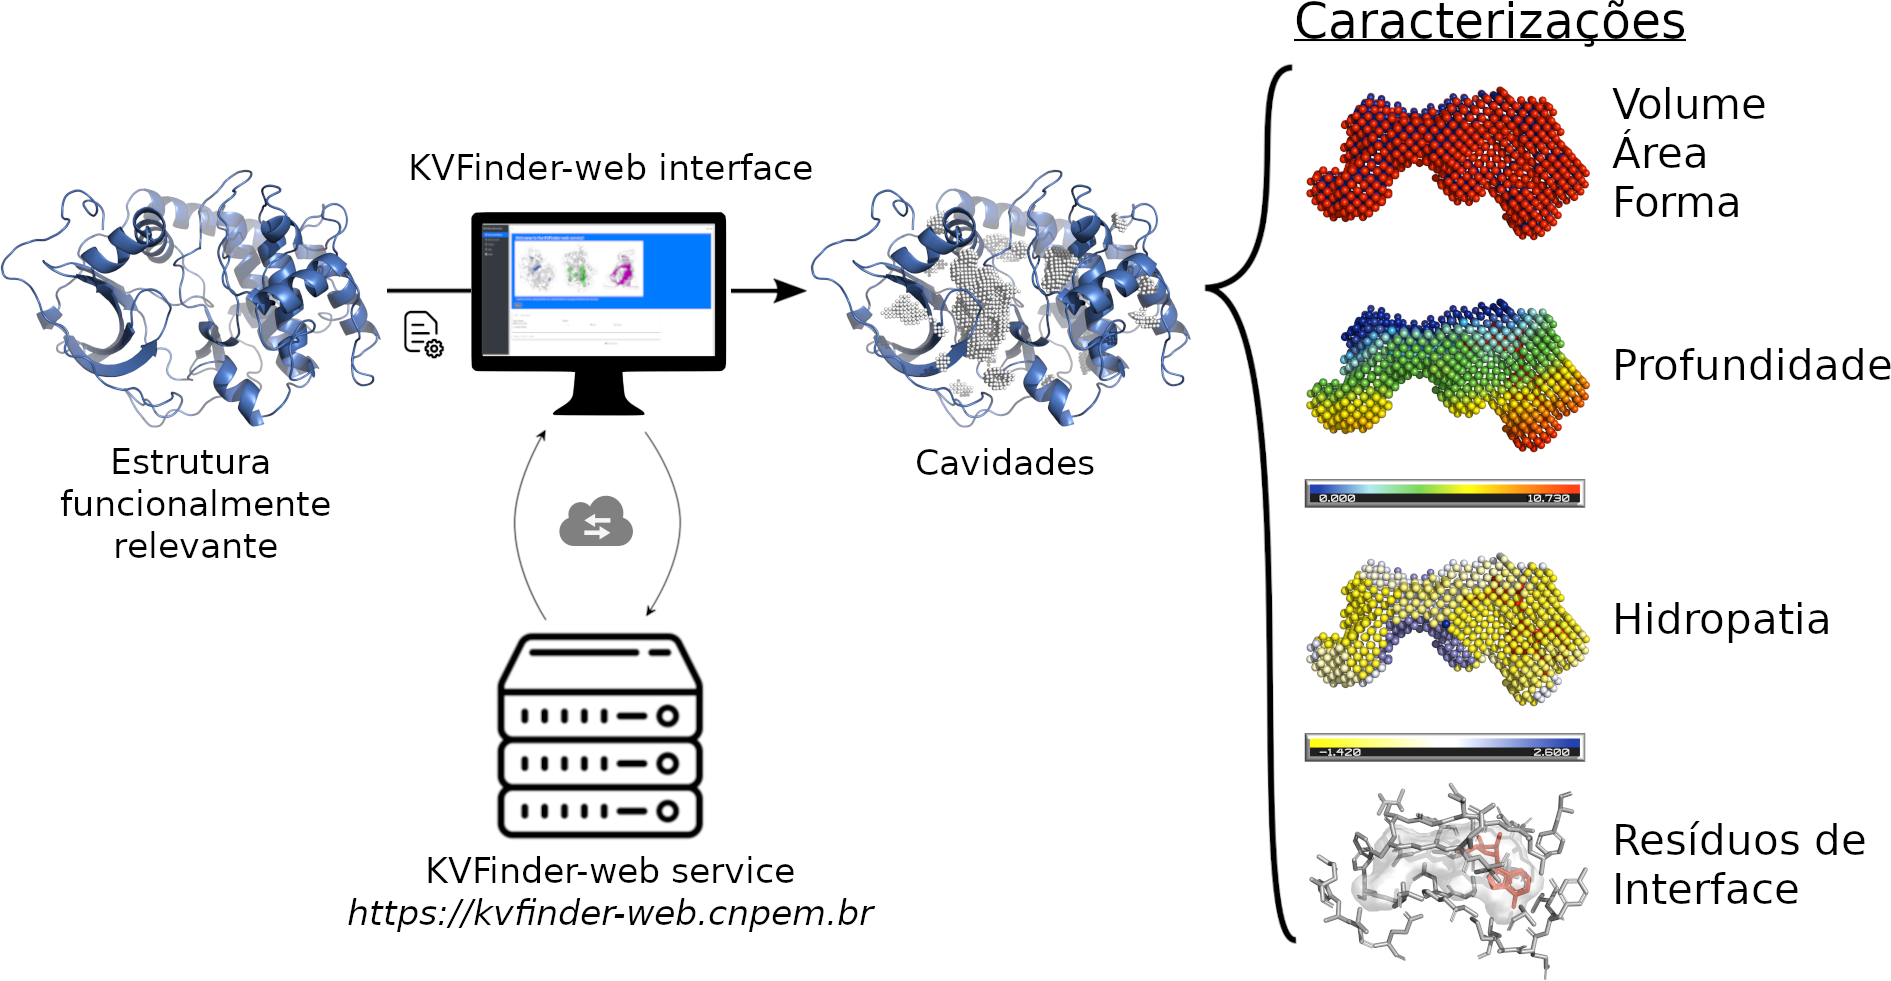
\includegraphics[scale=1.6]{images/kvweb-overview.png}
  \centerline{\tiny{\textbf{Source:} Adapted from \cite{guerra2023A}. Licensed under \href{https://creativecommons.org/licenses/by/4.0/}{CC BY 4.0}.}}
  \caption[Representative scheme of the KVFinder-web workflow to detect and characterize cavities in functionally relevant structures]{\textbf{Representative scheme of the KVFinder-web workflow to detect and characterize cavities in functionally relevant structures.}}
  \label{fig:kvweb-overview}
\end{figure}

Beyond the advancements in parKVFinder's performance and usability, the installation and configuration procedures of our cavity detection tool, alongside other independent tools, still present a significant barrier for users without the ideally required technical knowledge. Additionally, scientists, educators, and students may encounter limitations in their local computational resources, affecting the proper use of cavity detection and characterization methods. 

In this scenario, we introduced KVFinder-web \cite{guerra2023A}, an open-source web application for detecting and characterizing cavities in a wide range of biomolecular structures, including but not limited to proteins and nucleic acids. Subsequently, KVFinder-web was published in \textit{Nucleic Acids Research} \cite{guerra2023A} and released as KVFinder-web \href{https://github.com/LBC-LNBio/KVFinder-web/releases/tag/v1.1.0}{v1.1.0}, with the current version being \href{https://github.com/LBC-LNBio/KVFinder-web/releases/tag/v1.1.1}{v1.1.1}. Accessible at \url{https://kvfinder-web.cnpem.br}, KVFinder-web operates on a standard client-server architecture, consisting of two independent components: a RESTful web service (KVFinder-web service) and a graphical web interface (KVFinder-web portal). To further enhance the user experience, we also provide a graphical plugin for PyMOL (PyMOL KVFinder-web Tools). Next, we will describe each of these components in detail.

\subsection{KVFinder-web portal}

The KVFinder-web portal is an interactive graphical interface of KVFinder-web that provides users, especially those inexperienced, with an easy-to-use web application to run parKVFinder (\href{https://github.com/LBC-LNBio/parKVFinder/releases/tag/v1.2.0}{v1.2.0}) and analyze results through any web browser. Developed in R Shiny \cite{rshiny}, the KVFinder-web portal offers a simple, direct, robust, and interactive protocol for cavity analysis and visualization, requiring only a biomolecule in \acs{PDB} format or its corresponding \acs{PDB} code. 

\begin{figure}[H]
  \centering
  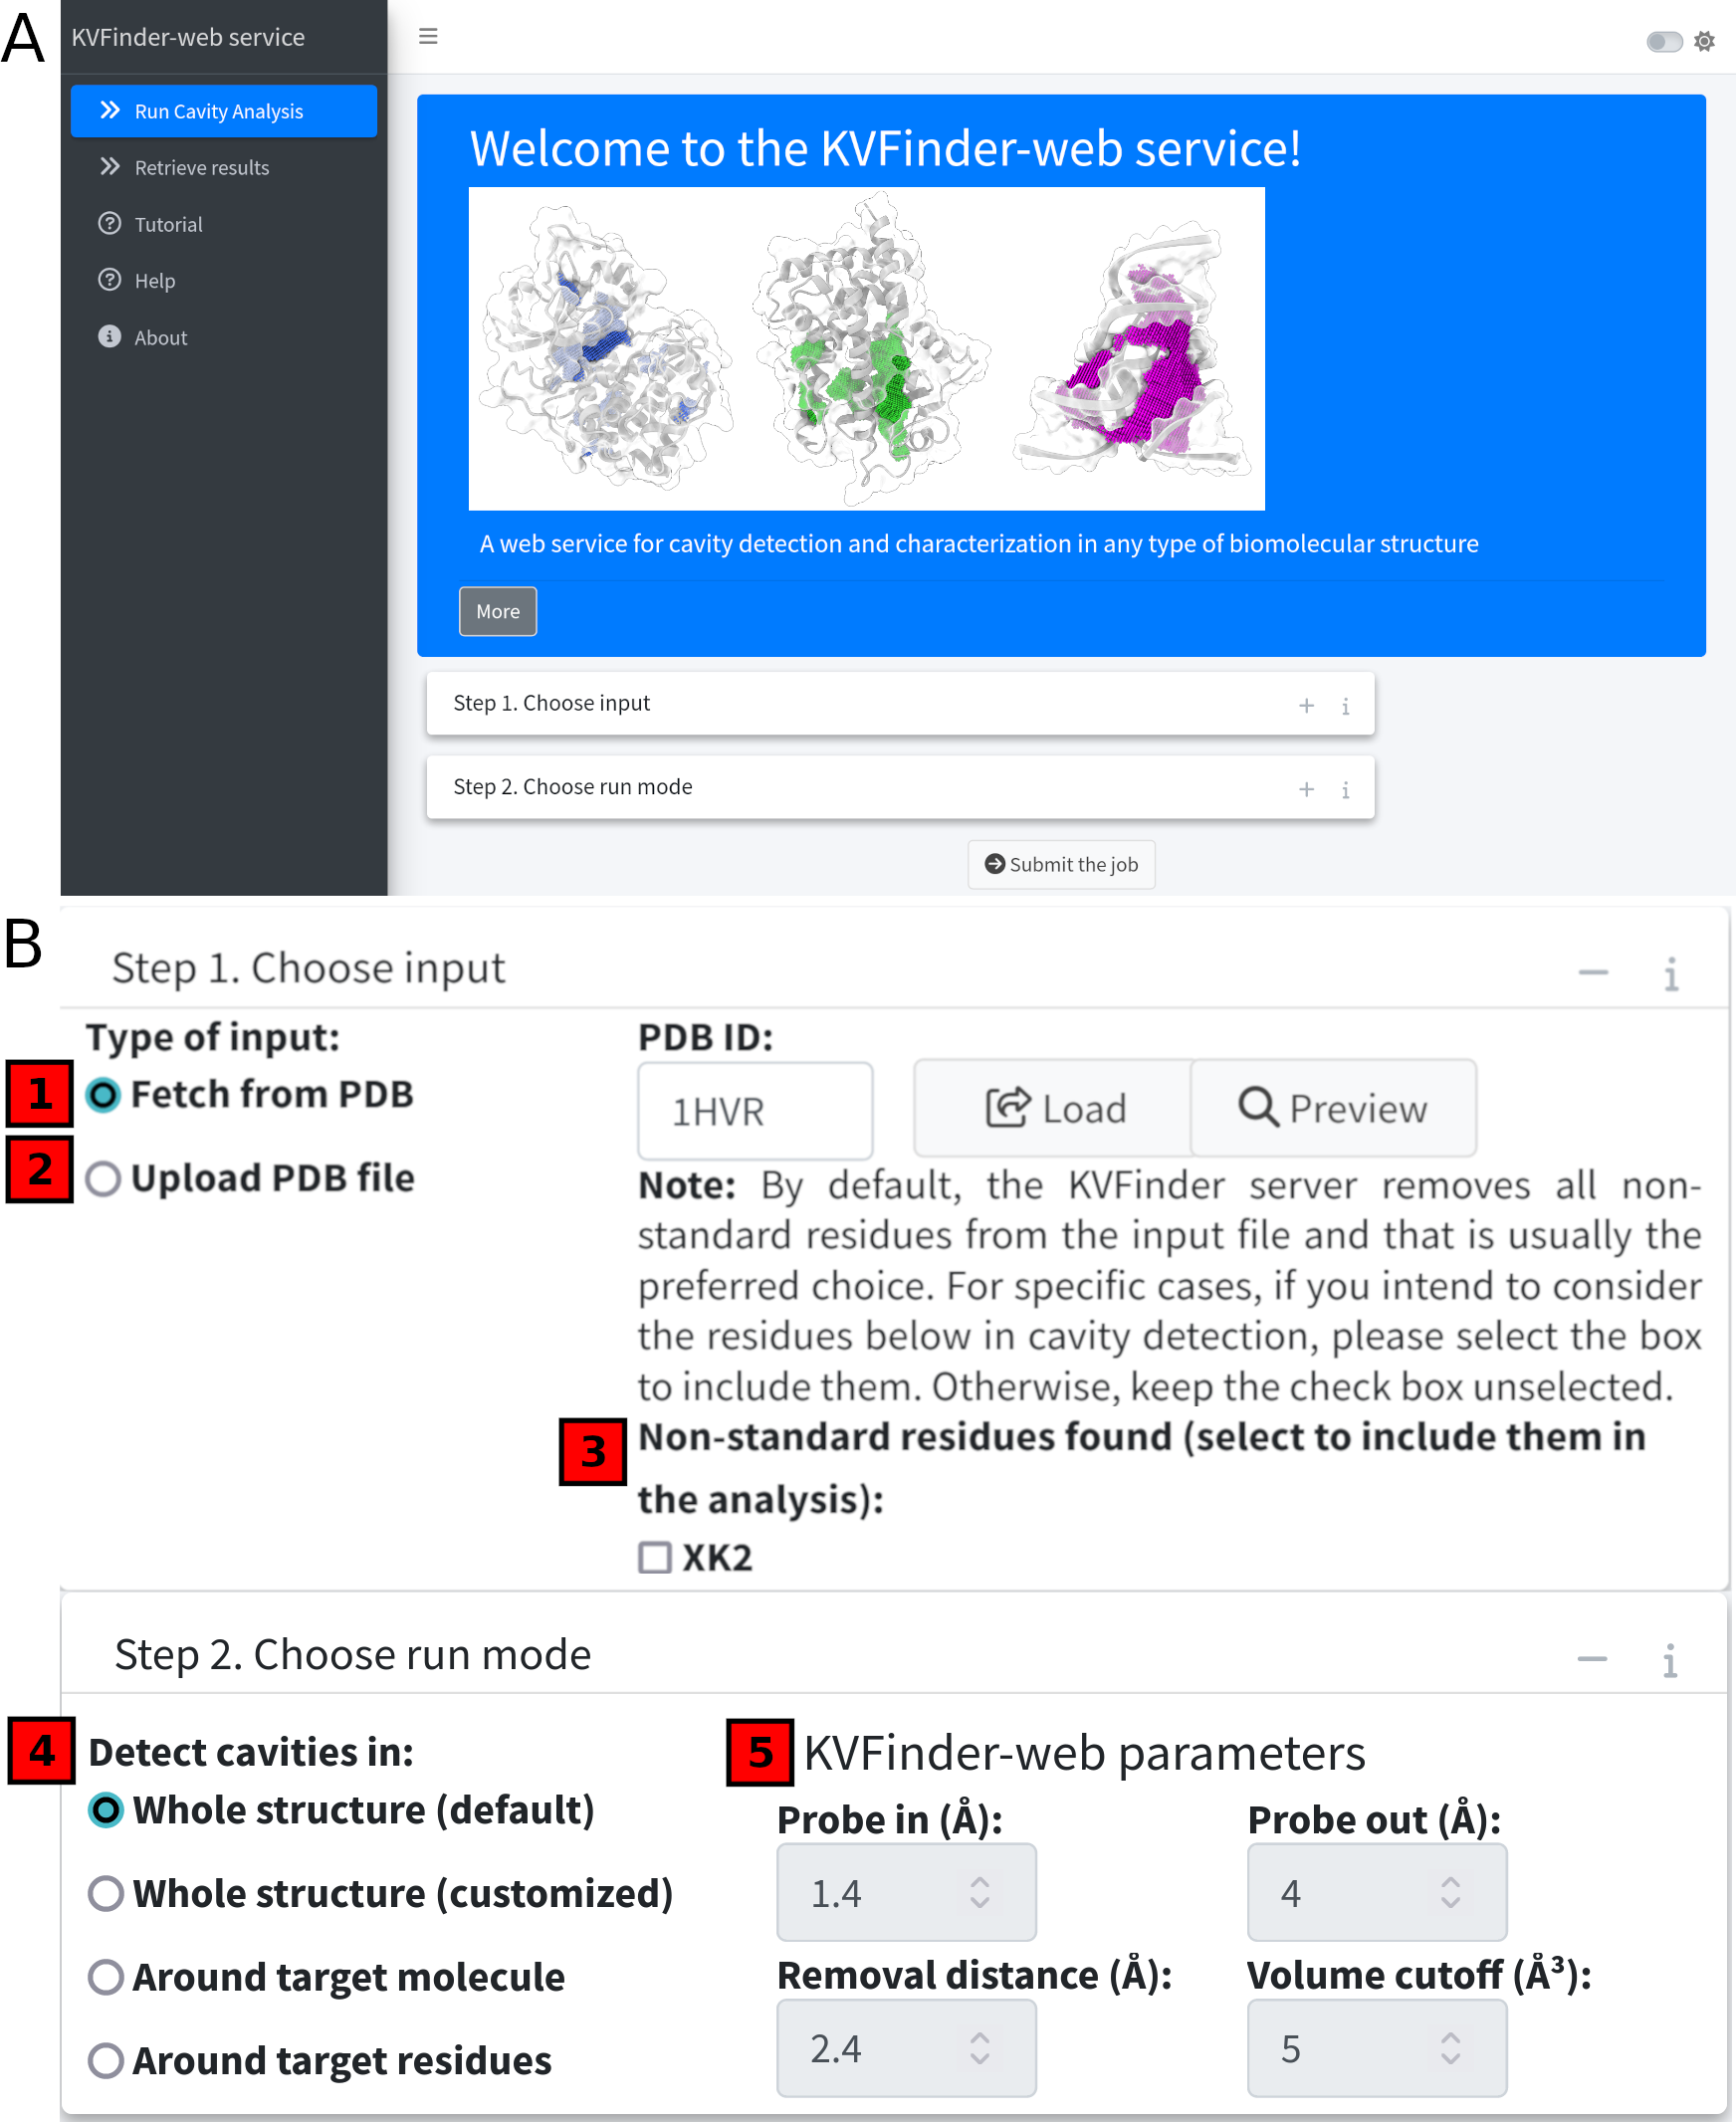
\includegraphics[scale=1]{images/kvweb-interface.png}
  \caption[KVFinder-web portal]{\textbf{KVFinder-web portal.} \textbf{(A)} Main page with the main tabs and sections for entering the target biomolecule and choosing the execution mode. \textbf{(B)} Detailed view of each step users must complete before submitting the target biomolecule for cavity analysis. The first step involves selecting the target biomolecule, which can be done by providing a PDB ID and searching the PDB database (1) or uploading a PDB file (2). After uploading the PDB, the KVFinder-web portal checks the PDB and informs about detected non-standard residues (3). In the next step, users must select a suitable execution mode (4) and customize, if necessary, the detection parameters (5).}
  \label{fig:kvweb-interface}
\end{figure}

The KVFinder-web portal was initially published in version \href{https://github.com/LBC-LNBio/KVFinder-web-portal/releases/tag/v1.1.0}{v1.1.0} in the \textit{Nucleic Acids Research} \cite{guerra2023A}. After collecting feedback from users, the graphical interface (Figure \ref{fig:kvweb-interface}) has undergone improvements in version \href{https://github.com/LBC-LNBio/KVFinder-web-portal/releases/tag/v1.1.1}{v1.1.1} to enhance user experience. Changes include revamping tab layouts, fixing critical bugs in the Retrieve Results tab, revising documentation for clarity, adding the LNBio/CNPEM logo, and aligning the color scheme with the LNBio institutional colors. These updates aim to provide a more polished and user-friendly KVFinder-web, ensuring visual consistency and addressing functional issues for a smoother user interaction. The source code is under continuous development and available at the following repository: \url{https://github.com/LBC-LNBio/KVFinder-web-portal}.
 

The interface provides the key functionalities of the KVFinder-web service, allowing users to upload a target biomolecule from a \acs{PDB} file or provide the corresponding \acs{PDB} code, and customize cavity detection parameters and execution modes (Figure \ref{fig:kvweb-interface}B). Four cavity detection modes are available, offering options that best suit users' cavity analysis needs:

\begin{itemize}
  \item \textbf{Whole structure (default)}: uses preset parameters to detect cavities across the whole biomolecular structure;
  \item \textbf{Whole structure (customized)}: allows users to customize the detection parameters for cavity detection across the whole biomolecular structure;
  \item \textbf{Around target molecule}: detects cavities around a chosen target molecule, focusing the search on the region surrounding that molecule, with customizable detection parameters;
  \item \textbf{Around target residues}: detects cavities within a custom box, defined by selecting specific residues within the target biomolecular structure, with customizable detection parameters.
\end{itemize}

Customizable detection parameters include \textit{Probe In}, \textit{Probe Out}, \textit{Removal Distance}, and \textit{Volume Cutoff} (Figure \ref{fig:kvweb-interface}B). In brief, \textit{Probe In} is a smaller probe (in \AA) that traverses the target biomolecule, defining its molecular surface (usually defined as a sphere the size of a water molecule - $1.4 \AA$), while \textit{Probe Out} is a larger probe (in $\AA$) that traverses the target biomolecule, defining regions of inaccessibility. Thus, cavities are defined as regions accessible to \textit{Probe In}, which are usually more inclusive but not to \textit{Probe Out}. \textit{Removal Distance} is a distance (in $\AA$) for removing cavity points from the cavity-border midpoint to delimit the outer limits of the cavity. \textit{Volume Cutoff} is a cavity volume filter (in $\AA^3$) to exclude cavities with volumes smaller than this limit, typically considered as functionally irrelevant cavities. For a more detailed explanation of each parameter, refer to the references \cite{oliveira2014,guerra2019,guerra2020,guerra2021,guerra2023A}.
 
Additionally, the graphical interface allows users to download and visualize results easily and interactively (Figure \ref{fig:kvweb-results}). Morphological (\ie, volume, area, and depth) and physicochemical (\ie, hydrophobicity) characterizations of each cavity are displayed in an interactive table, available for download in TOML format. A biomolecule viewer, powered by the graphical engine NGL for R (NGLVieweR \cite{nglviewerr}), displays the biomolecular structure with its cavities, available for download in \acs{PDB} format, and allows various customizations, such as highlighting cavities and displaying interface residues around them.

\begin{figure}[h]
  \centering
  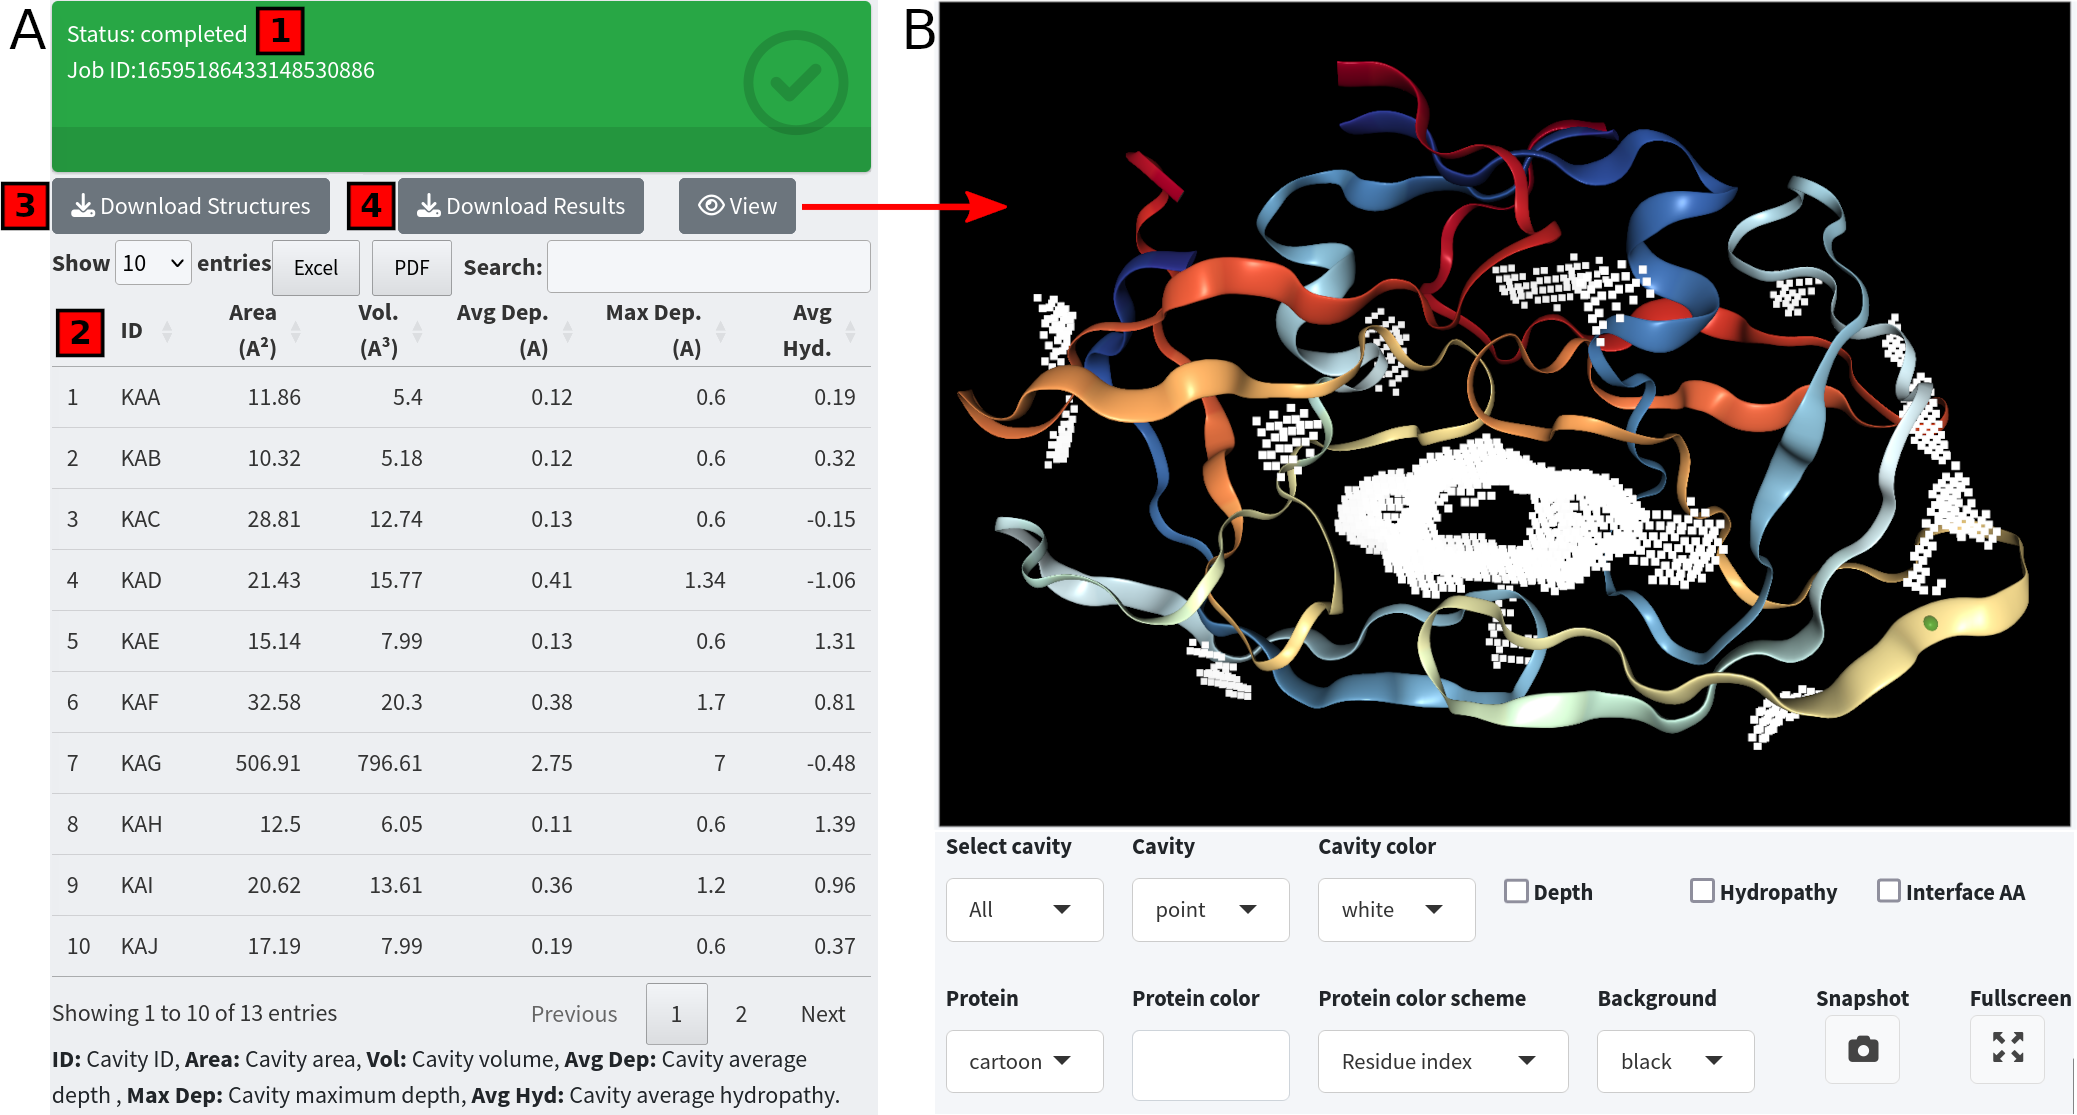
\includegraphics[scale=1.8]{images/kvweb-results.png}
  \centerline{\tiny{\textbf{Source:} Reprinted from \cite{guerra2023A}. Licensed under \href{https://creativecommons.org/licenses/by/4.0/}{CC BY 4.0}.}}
  \caption[Results visualization in KVFinder-web portal]{\textbf{Results visualization in KVFinder-web portal.} \textbf{(A)} Results section of the KVFinder-web portal. The job status box (green: 'completed'; yellow: 'running' or 'queued'; red: 'cancelled') (1). Upon completion, the interface presents the results in a table, including volume, area, average depth, maximum depth, and average hydrophobicity of the cavities (2). Users can download a ZIP file containing the target biomolecule and PDB files of the cavities (3) or a TOML file with cavity characterizations (4). \textbf{(B)} The target biomolecule with cavities can be viewed by clicking the 'View' button, and users can customize the visualization of the biomolecule and cavities.}
  \label{fig:kvweb-results}
\end{figure}

\subsection{KVFinder-web service}

The KVFinder-web service is a RESTful web service that employs parKVFinder (\href{https://github.com/LBC-LNBio/parKVFinder/releases/tag/v1.2.0}{v1.2.0}) to detect and characterize cavities in biomolecular structures, as described in \cite{guerra2019,guerra2020,guerra2023A}. Operating on a Web-Queue-Worker architecture (Figure \ref{fig:kvweb-service-architecture}), it handles HTTP requests and responses from the web interface, manages jobs, and executes parKVFinder on accepted jobs. Currently, KVFinder-web service is in version \href{https://github.com/LBC-LNBio/KVFinder-web-service/releases/tag/v1.1.1}{v1.1.1}. The source code is under continuous development and available at the following repository: \url{https://github.com/LBC-LNBio/KVFinder-web-service}.

\begin{figure}[h]
  \centering
  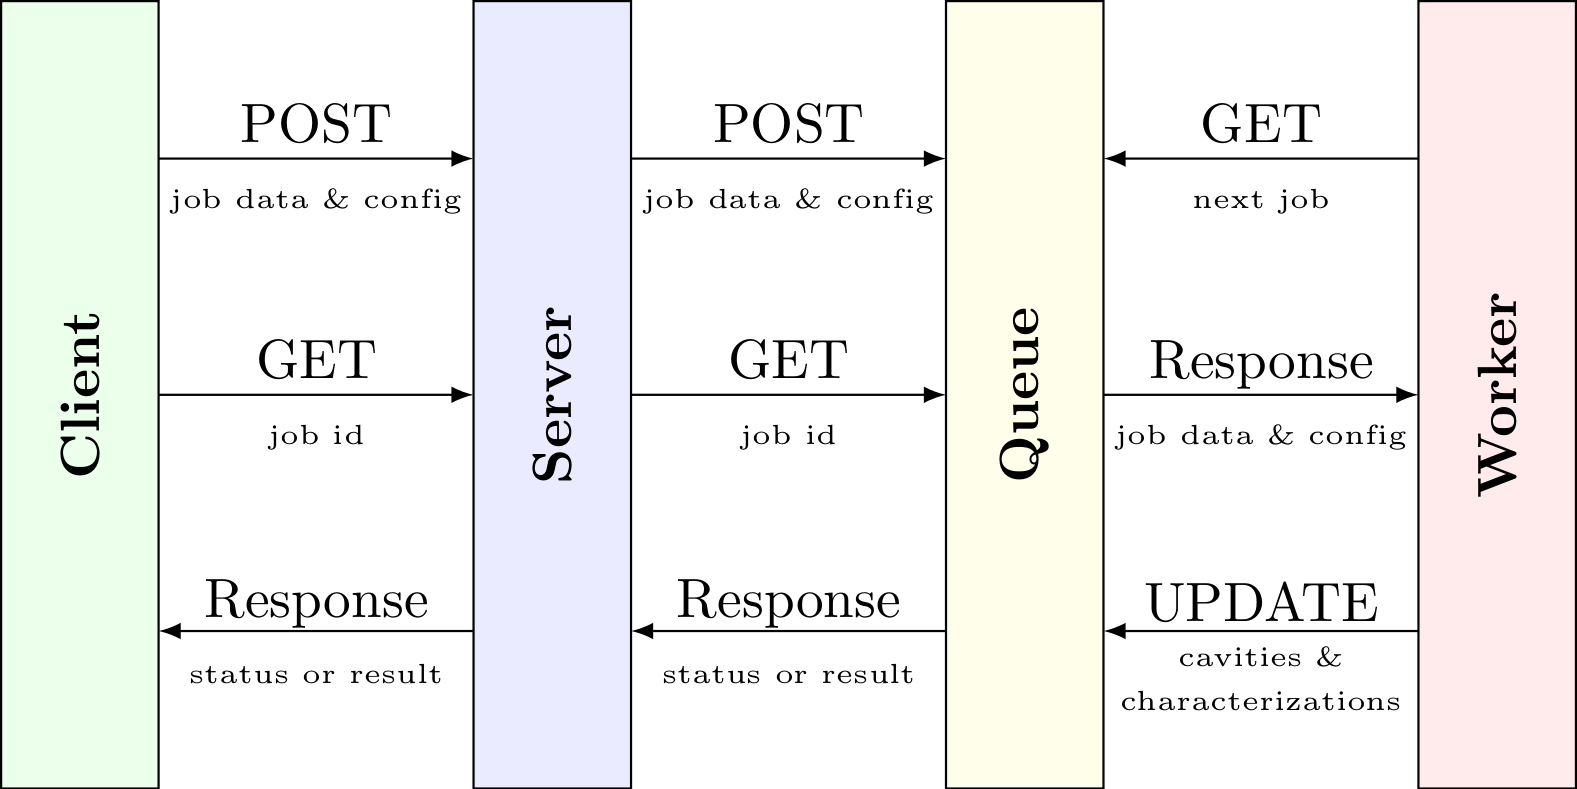
\includegraphics[scale=1.5]{images/web-queue-worker-architecture.png}
  \caption[KVFinder-web service architecture and communication]{\textbf{KVFinder-web architecture and communication.}}
  \label{fig:kvweb-service-architecture}
\end{figure}

The KVFinder-web service, written in Rust, comprises three modules: the \textit{Web server}, the \textit{Queue}, and the \textit{Worker}. The \textit{Web server} module, employing the Actix web framework (\url{https://actix.rs}), receives job requests via HTTP POST with a JSON-based configuration file containing molecular structures and parKVFinder detection parameters. The molecular structures of a target receptor and optionally a target ligand are stored in \textit{pdb} and \textit{pdb\_ligand} attributes of the JSON, respectively, as \acs{PDB}-formatted strings. Valid requests prompt the \textit{Web server} to return a response with a unique identifier, created using a hash function based on the incoming JSON data. In case of an invalid request, an HTTP error code with an error message is returned. The job ID creation through a hash function ensures that cached results are retrieved upon resenting a request.

Jobs accepted by the \textit{Web server} are sent to the \textit{Queue} module, an Ocypod job queue server instance (\url{https://github.com/davechallis/ocypod}), where they await processing by a \textit{Worker} module. The \textit{Worker} module communicates with the \textit{Queue} module, requesting the next job to be processed by parKVFinder software. To prevent resource exhaustion, some parKVFinder parameters are constrained or even pre-defined. Upon job completion, the cavity analysis (cavities and their characterizations) is sent back to the \textit{Queue} module, updating the job status and results, which are made available to clients through the \textit{Web server} module. 

Retrieving job results involves sending an HTTP GET request with the job ID, and the \textit{Web server} returns the current job status - \'queued\', \'running\', or \'completed\' - along with the corresponding results, if available. Each job remains cached in the queue for one day after completion. Depending on processing requirements, additional worker modules can be allocated to enable the simultaneous processing of multiple jobs. Each module of the KVFinder-web service is packaged into a Docker container \cite{docker}, making it available for execution in local or cloud computing environments. These modules are combined in a Docker Compose file for easy deployment.

The computational performance of the KVFinder-web service was also evaluated on kv1000 \cite{guerra2020}, varying two crucial parameters related to cavity detection: \textit{Probe Out} and \textit{Removal Distance} (Figure \ref{fig:kvweb-performance}). Varying the \textit{Probe Out} parameter creates a coarser molecular surface around the biomolecular structure, delineating the cavity-solvent boundary. Increasing the \textit{Probe Out} reduces the degree of accessibility of the molecular surface and increases the calculation time in the KVFinder-web service. Conversely, the \textit{Removal Distance} parameter removes cavity points close to the boundary, aiding in the identification of sub-cavities and surface cavities. The runtime does not exhibit a clear relationship with the \textit{Removal Distance} parameter, as it is influenced by the size of the boundary and the number of cavities, not the number of atoms. Generally, the runtime increases linearly with the number of atoms in the target biomolecular structure within the 3D grid.

\begin{figure}[h]
  \centering
  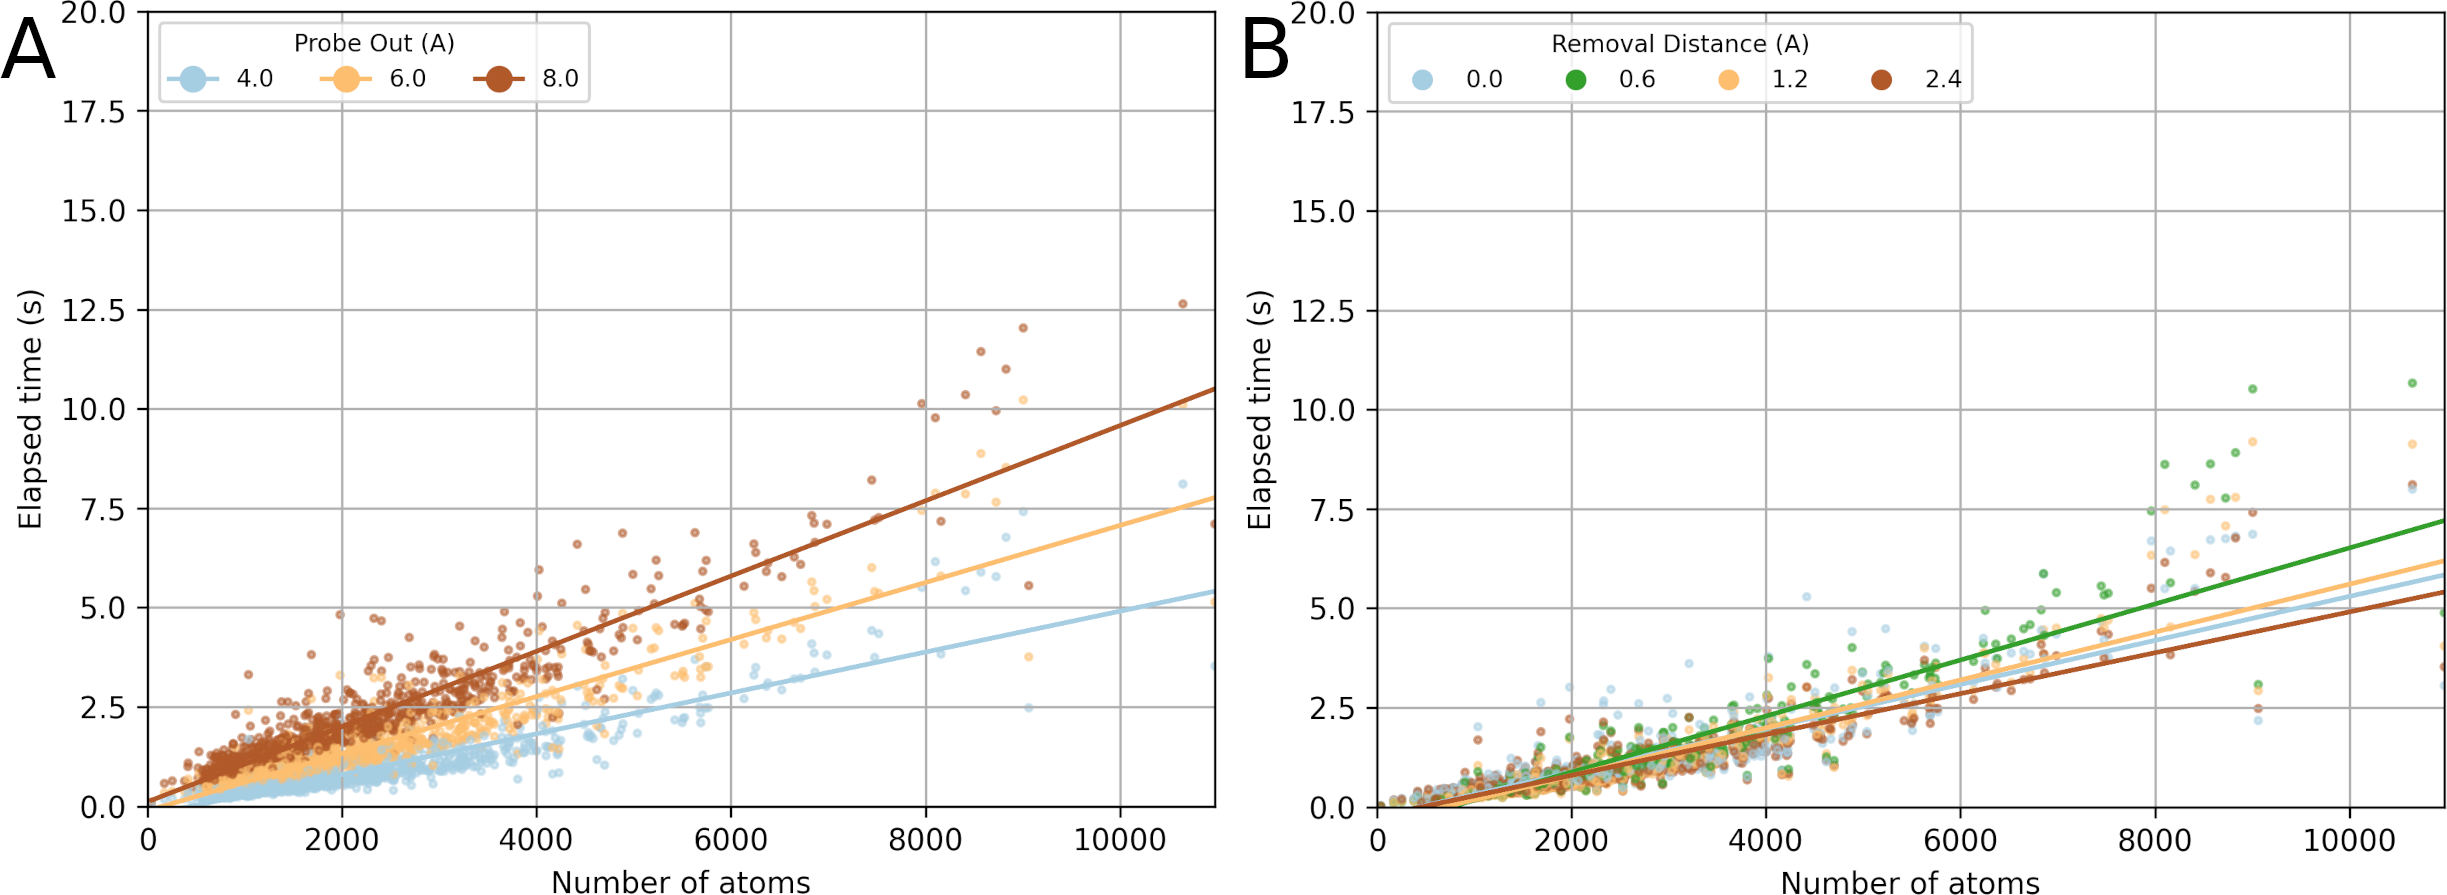
\includegraphics[scale=1.6]{images/kvweb-performance.png}
  \centerline{\tiny{\textbf{Source:} Reprinted from \cite{guerra2023A}. Licensed under \href{https://creativecommons.org/licenses/by/4.0/}{CC BY 4.0}.}}
  \caption[Effects of detection parameters on KVFinder-web service performance]{\textbf{Effects of detection parameters on KVFinder-web service performance.} Cavity detection was performed on kv1000 \cite{guerra2020}, varying \textbf{(A)} \textit{Probe Out} sizes and \textbf{(B)} \textit{Removal Distance}. Elapsed time relative the number of atoms in the target structure was recorded. Calculations were performed on a computer with an AMD Ryzen 7 1700 8-core, 3.0 GHz processor, 32GB of RAM, running Ubuntu 22.04 LTS.}
  \label{fig:kvweb-performance}
\end{figure}

\subsection{PyMOL KVFinder-web Tools}

For users familiar with PyMOL \cite{pymol}, the \textbf{PyMOL KVFinder-web Tools} (Figure \ref{fig:pymol-kvweb-tools}), developed in Python3 and Qt, integrates the KVFinder-web service with the molecular visualization program. This user-friendly \acs{GUI} allows customization of detection parameters for a target biomolecular structure and sends jobs to a configured KVFinder-web service (Figure \ref{fig:pymol-kvweb-tools}A). Currently, PyMOL KVFinder-web Tools is in version \href{https://github.com/LBC-LNBio/PyMOL-KVFinder-web-Tools/releases/tag/v1.0.0}{v1.0.0}. The source code is available at the following repository: \url{https://github.com/LBC-LNBio/PyMOL-KVFinder-web-Tools}.

Similar to the parKVFinder plugin for PyMOL \cite{guerra2020}, the search space can be adjusted to a custom box (box adjustment mode) and/or a radius around a ligand or target molecule (ligand adjustment mode), instead of detecting and characterizing cavities across the entire biomolecular surface (whole protein mode). Upon successful submission, accepted jobs are routinely and asynchronously requested from the KVFinder-web service. When a job is completed, the plugin automatically processes the received data, cavities, and characterizations into local files and makes them available in the GUI. This graphical plugin operates similarly to the KVFinder-web portal; characterizations are displayed in lists (Figure \ref{fig:pymol-kvweb-tools}B), and cavities are customized based on their properties in the PyMOL viewer (Figure \ref{fig:pymol-kvweb-tools}C and D). However, jobs submitted in the KVFinder-web portal can be loaded into PyMOL KVFinder-web Tools and vice versa.

\begin{figure}[H]
  \centering
  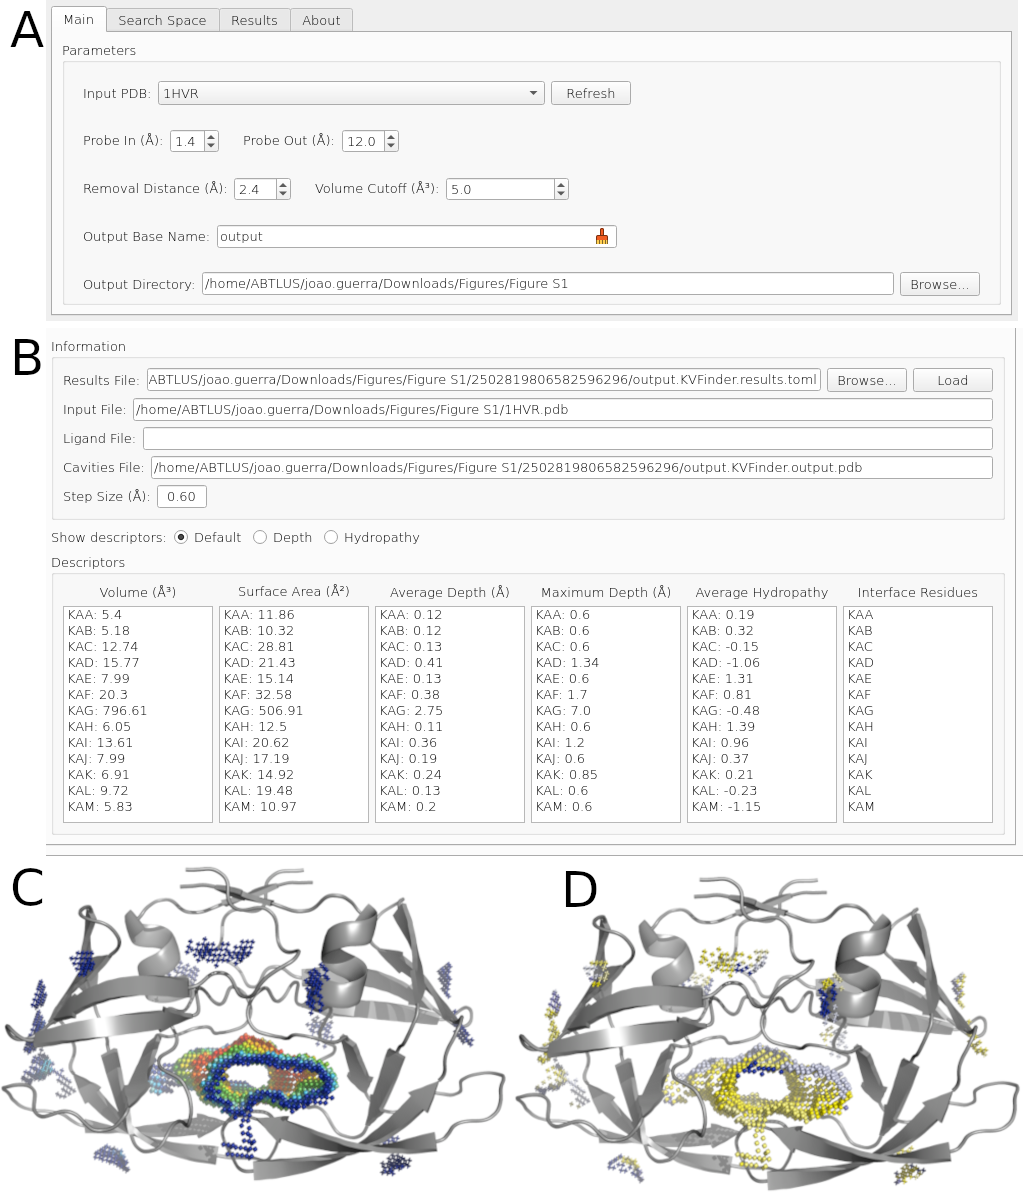
\includegraphics[scale=3.5]{images/pymol-kvweb-tools.png}
  \centerline{\tiny{\textbf{Source:} Reprinted from \cite{guerra2023A}. Licensed under \href{https://creativecommons.org/licenses/by/4.0/}{CC BY 4.0}.}}
  \caption[PyMOL KVFinder-web Tools]{\textbf{PyMOL KVFinder-web Tools.} Cavity detection in the HIV-1 protease structure (PDB ID: 1HVR), with \textit{Probe Out} set to 12 Å. \textbf{(A)} Main parameters tab containing detection parameters and molecular structures to explore. \textbf{(B)} Visualization tab displaying data received (cavities and characterizations) from the KVFinder-web service shown in the \acs{GUI}. \textbf{(C)} Depth characterization and \textbf{(D)} Eisenberg & Weiss hydrophobicity characterization, highlighting the active site (KAG cavity) in the \acs{GUI} and PyMOL viewer.}
  \label{fig:pymol-kvweb-tools}
\end{figure}

% TODO: revisar valores antes da publicação

\subsection{Monitoring and Analytics}

The monitoring and analytics of KVFinder-web are essential to ensure the web application's optimal functionality and deliver a high-quality user experience. This process provides valuable insights into user interaction, enabling maintainers and developers to tailor improvements and updates to user requirements. For a comprehensive approach, we implemented a monitoring process to track job execution and user behavior over time. 

Job submission tracking provides valuable information into system usage patterns, helping identify peak demand periods and optimize resources for smooth and efficient user experience. Additionally, it helps in assessing user adherence to our platform and gauging the impact of new features and updates. From March 1, 2023, to December 4, 2023, KVFinder-web executed 1,060 jobs, averaging of $\sim$106 jobs per month (Figure \ref{fig:job-execution}). During the developmental phase from March 2023 to May 2023, when KVFinder-web was accessible only to internal users from CNPEM, it averaged $\sim$65 jobs per month. After its public release in June 2023, alongside its publication in \textit{Nucleic Acids Research} \cite{guerra2023A}, KVFinder-web had an average of $\sim$124 jobs per month, indicating user adherence and the publication's impact.

\begin{figure}[h]
  \centering
  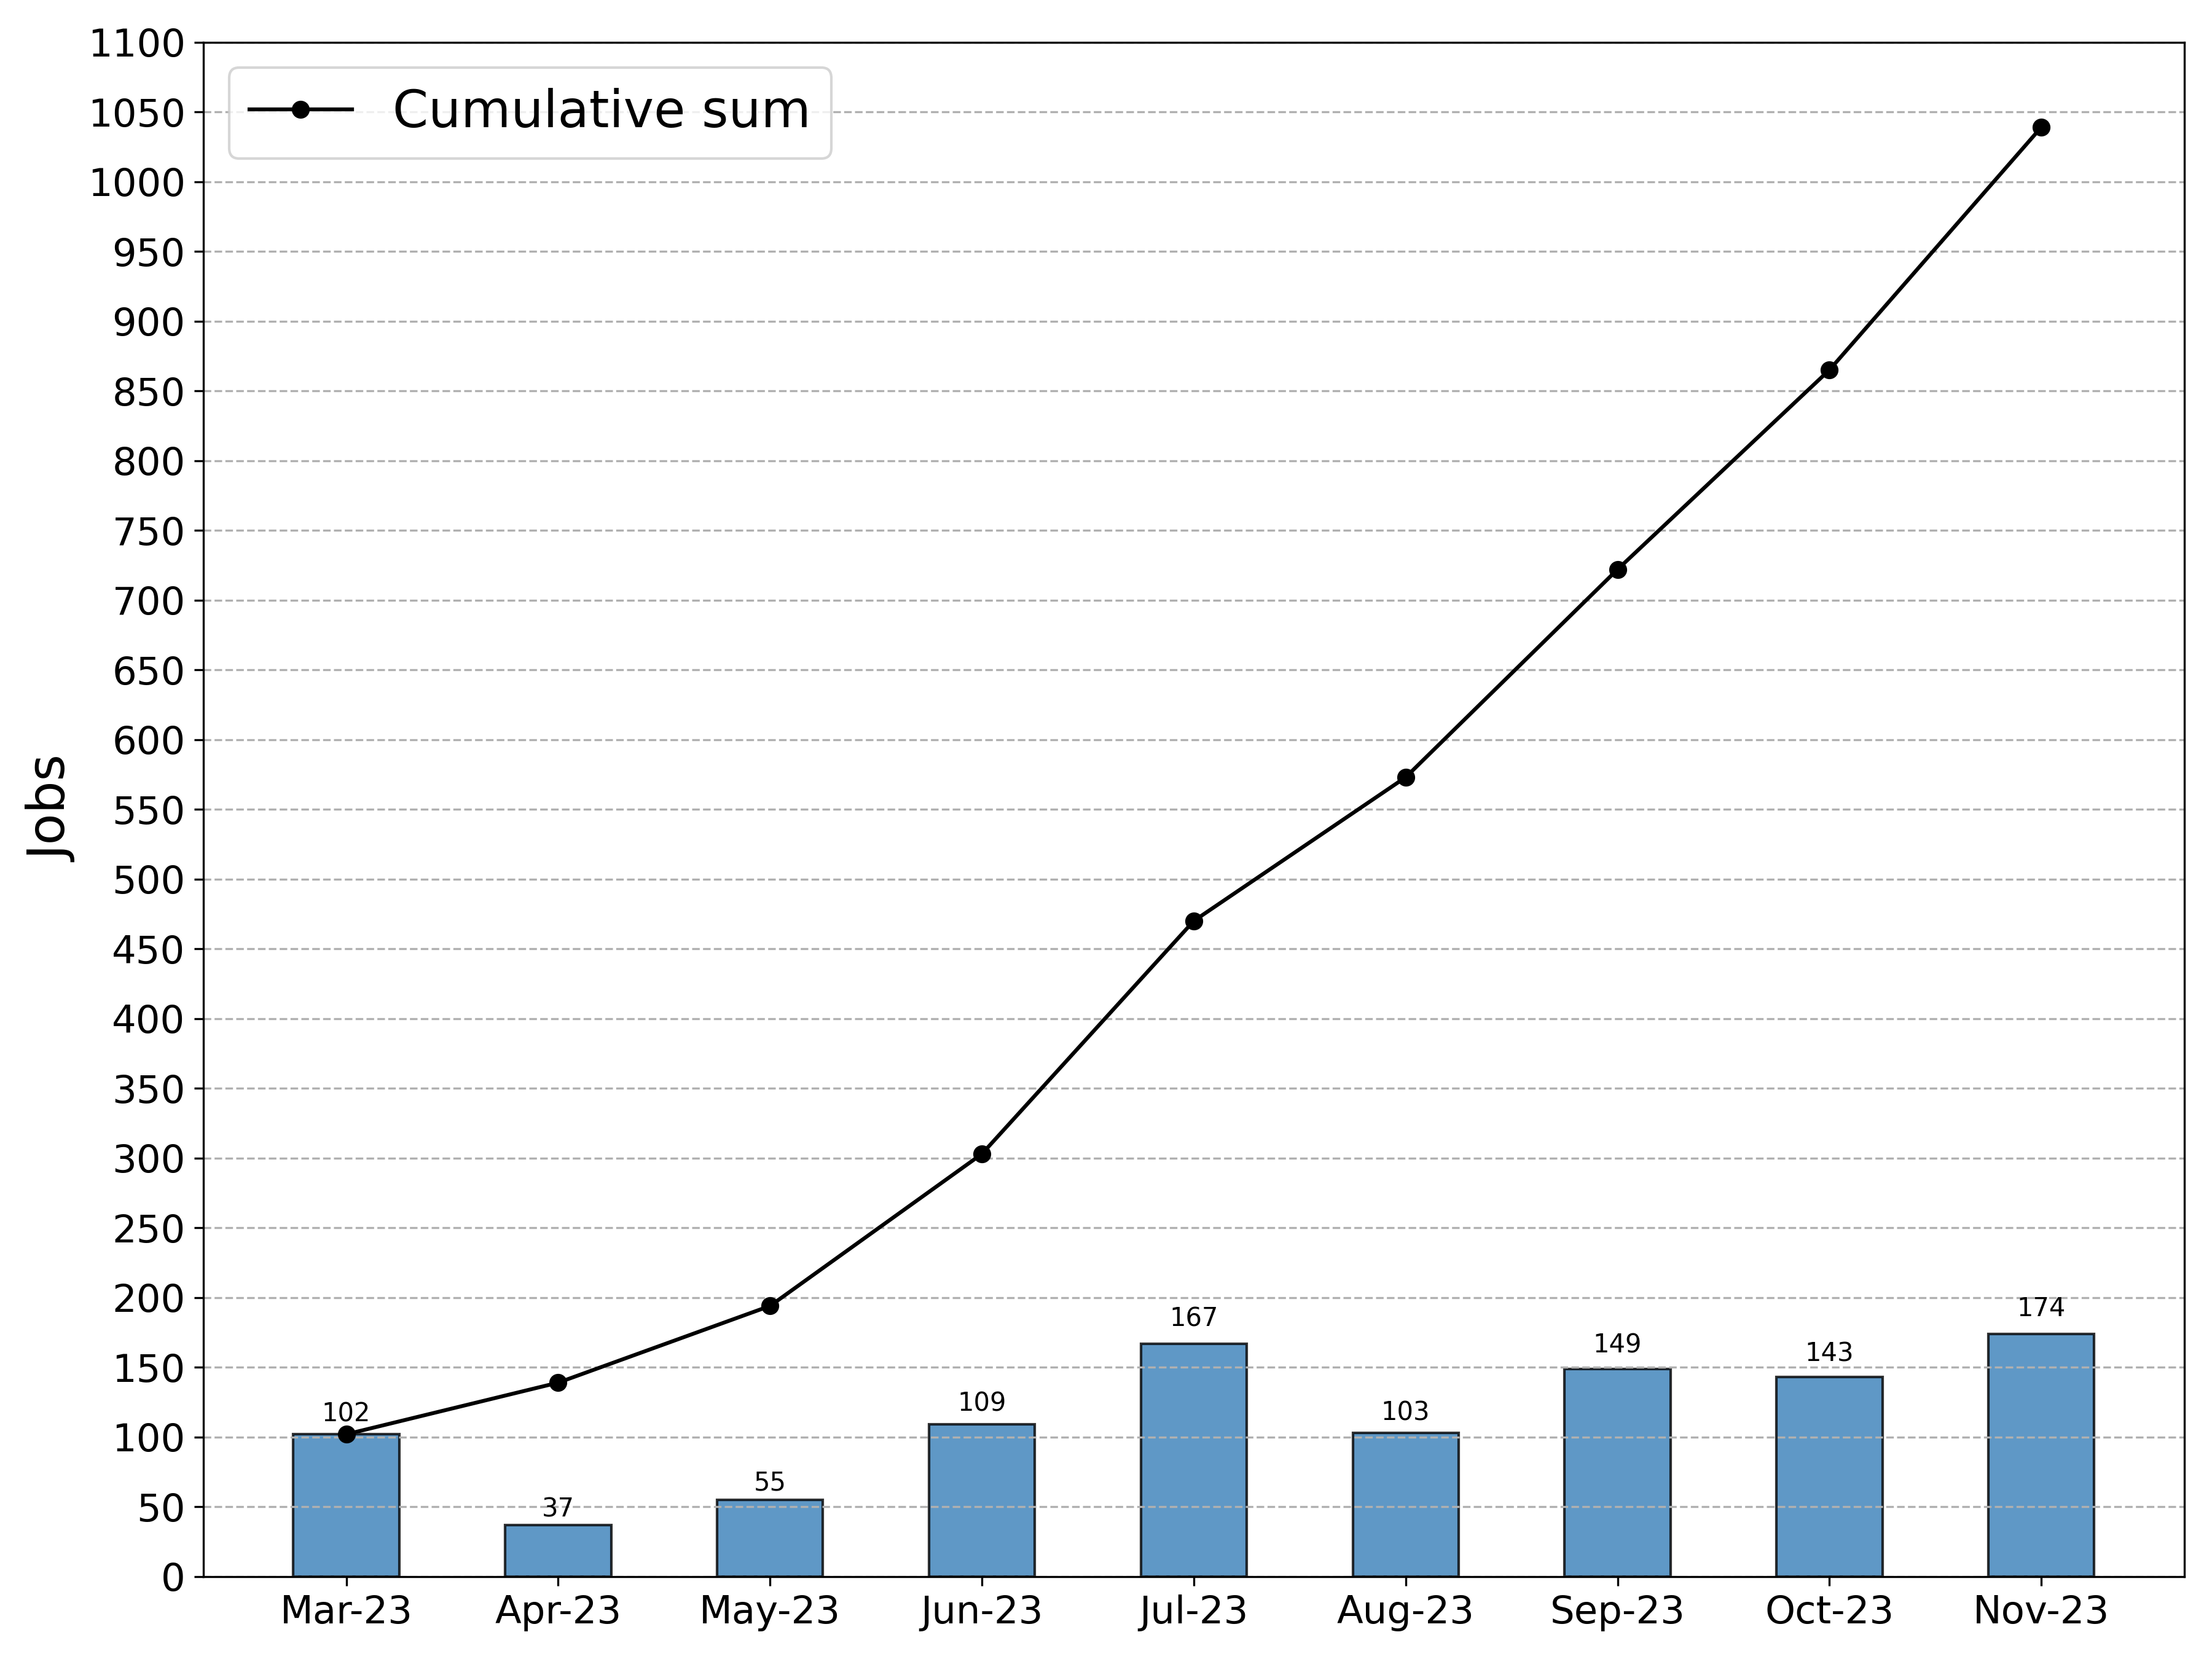
\includegraphics[scale=0.5]{images/jobs-executed-per-month.png}
  \caption[Jobs executed in KVFinder-web]{\textbf{Jobs executed in KVFinder-web.} Accepted jobs executed in KVFinder-web per month and their cumulative sum.}
  \label{fig:job-execution}
\end{figure}

Understanding user behavior through analytics is crucial for KVFinder-web development and maintenance, guiding iterative improvements, optimizing interface design, identifying popular features, and ensuring a smooth and efficient user experience. Initially, Cloudflare (\url{https://www.cloudflare.com}) was explored for user behavior analytics, but its collected data did not provide the desired insights due to its broader focus on content delivery, security, and performance services. Its monitoring capabilities are more centralized around overall website health and security. From October 21th, 2023 to November 21th, 2023, Cloudflare recorded 1,130 visitors, mainly from the United States (38.56\%), Netherlands (19.20\%), Germany (9.58\%), China (7.21\%), Spain (1.83\%), and Portugal (1.83\%). 

Subsequently, Microsoft Clarity (\url{https://clarity.microsoft.com}) emerged as a more suitable solution, offering a privacy-focused analytics tool that does not collect personal information (\eg, IP addresses or cookies). Leveraging Microsoft Clarity allowed for a deeper analysis of user interactions, offering valuable insights into navigation and engagement (\eg, click tracking, heatmaps, masked session recordings, and engagement metrics). Since its implementation from November 21, 2023 to December 4, 2023, KVFinder-web received 60 visitors, with 30 unique users from different countries, primarily Brazil (26.67\%), United States(26.67\%), Spain(10\%), Korea (10\%), and China (6.67\%) (Figure \ref{fig:clarity-analytics}A). Notably, the release of KVFinder-web has broadened our user base beyond Linux users, as users from different operating systems, such as Windows and MacOS, are now adopting KVFinder-web for cavity analysis (Figure \ref{fig:clarity-analytics}B). The average active session time was 7.0 minutes, with a variety of browsers being used (Figure \ref{fig:clarity-analytics}C). Microsoft Clarity has consistently provided valuable insights into user behavior, aiding in refining the user experience and addressing potential pain points. The data collected indicates that KVFinder-web is democratizing of parKVFinder in the structural biology community, with users worldwide and an average of $\sim$124 jobs per month since its official release.

\begin{figure}[h]
  \centering
  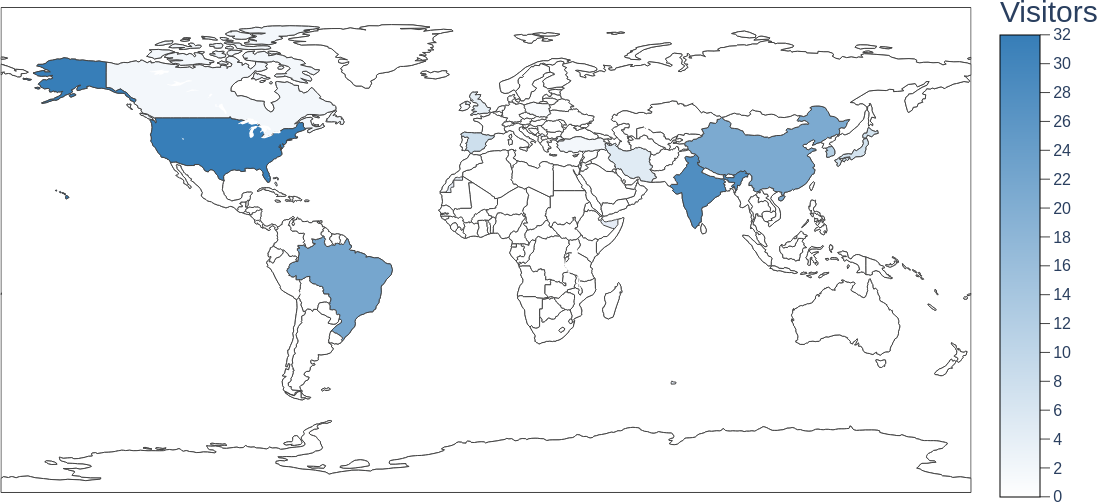
\includegraphics[scale=0.375]{images/clarity-monitoring/clarity-countries.png}
  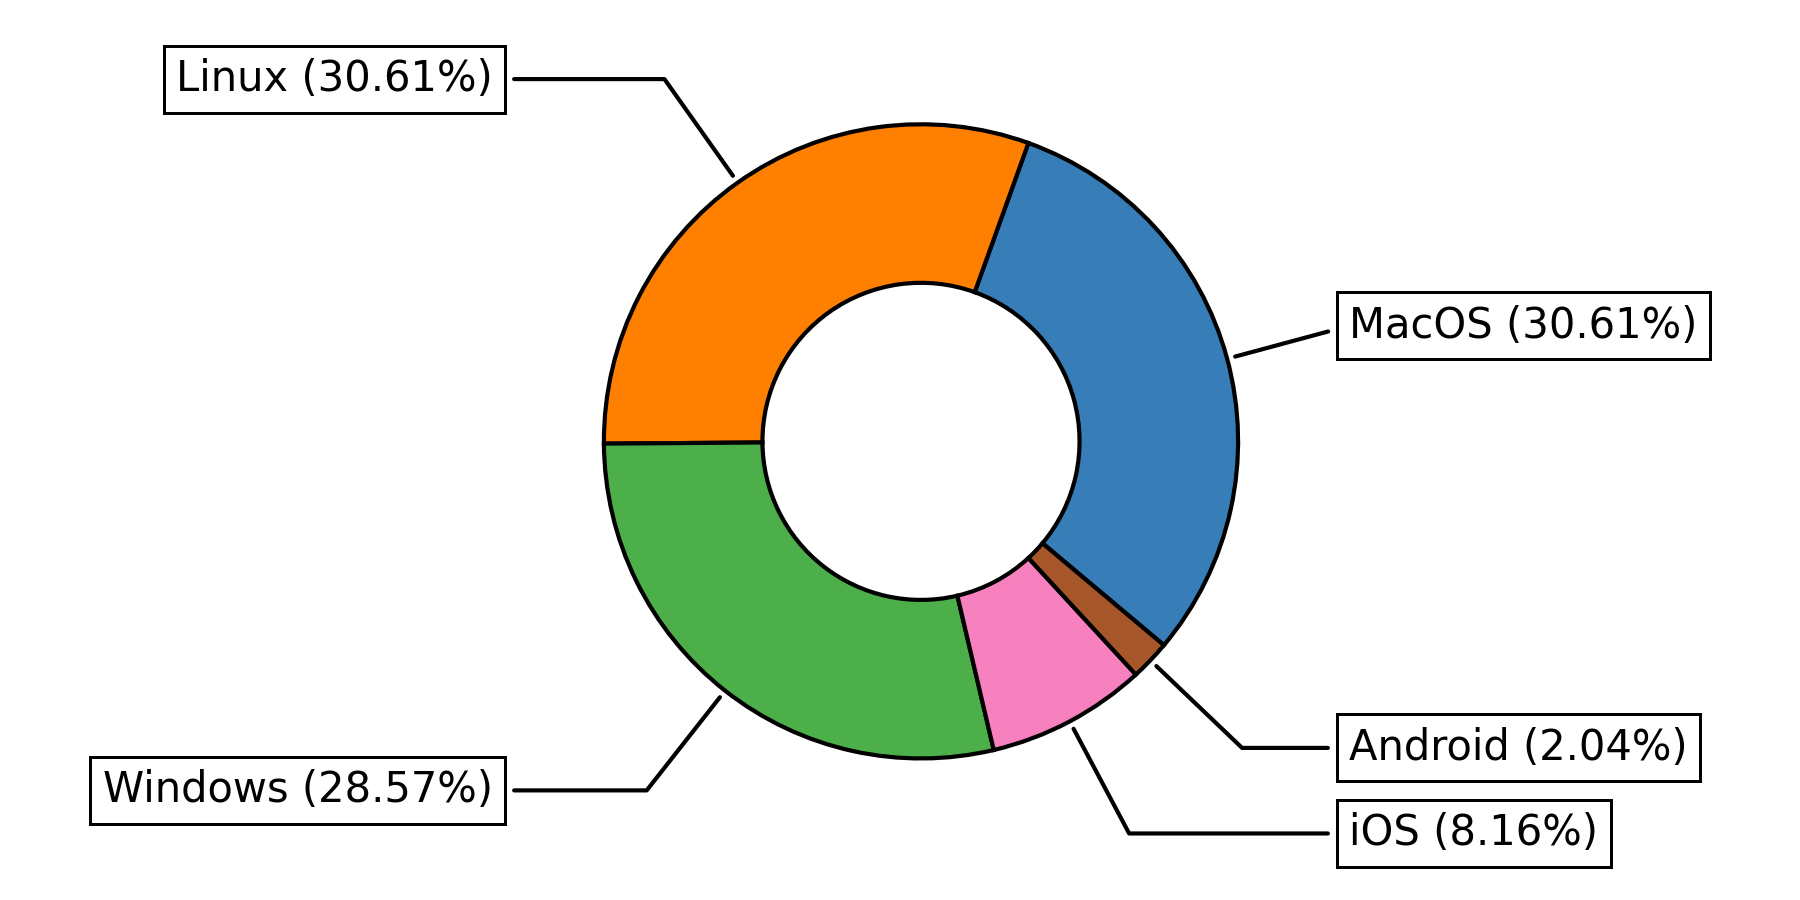
\includegraphics[scale=0.49]{images/clarity-monitoring/clarity-os.png}
  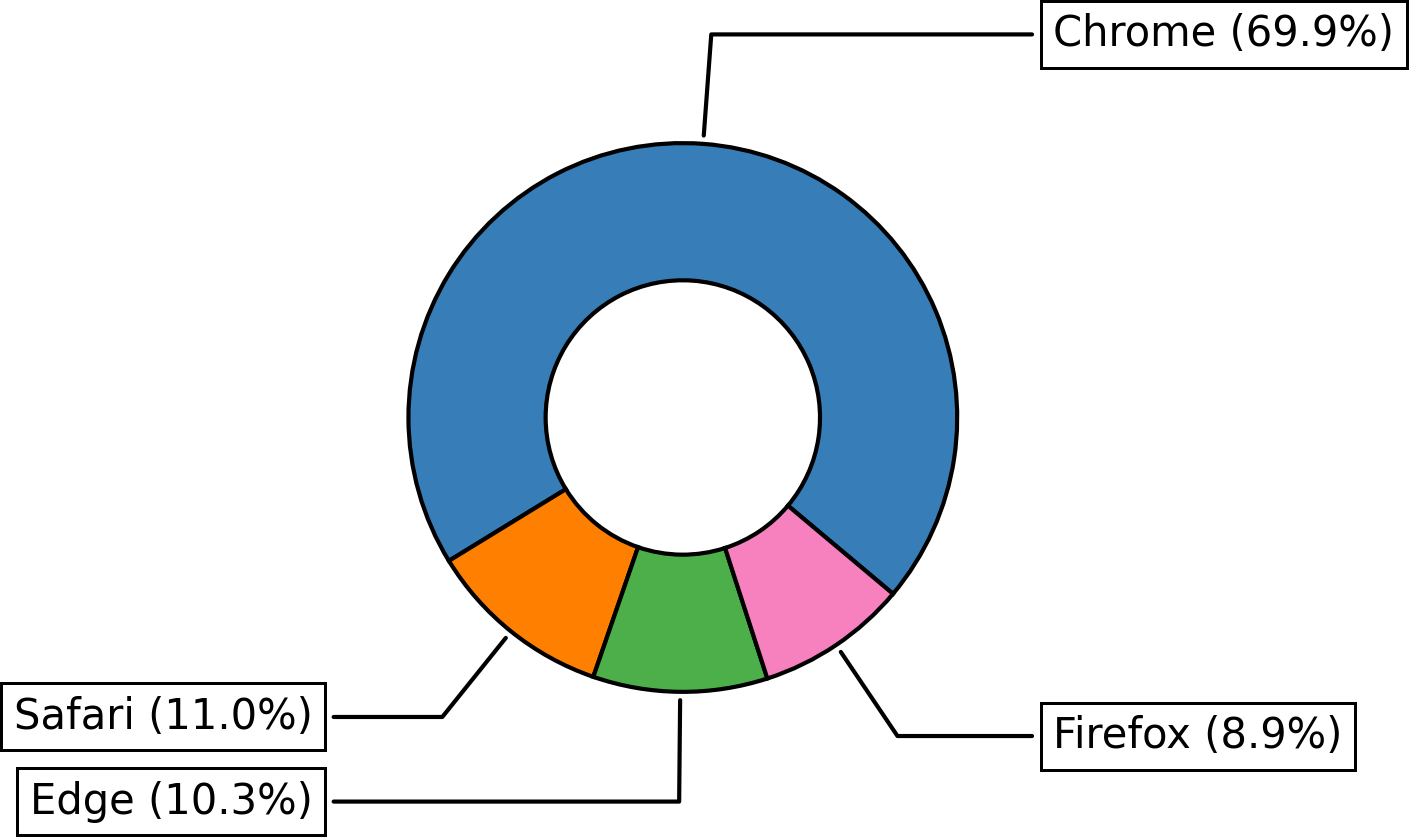
\includegraphics[scale=0.49]{images/clarity-monitoring/clarity-browsers.png}
  \caption[KVFinder-web user behaviour analytics]{\textbf{KVFinder-web user behaviour analytics.} \textbf{(A)} Countries. \textbf{(B)} Operating systems. \textbf{(C)} Browsers.}
  \label{fig:clarity-analytics}
\end{figure}

Finally, a crucial consideration in this monitoring process is data privacy. Recognizing the sensitivity of user data, stringent measures have been implemented to uphold privacy standards. Importantly, no one in the maintainer and developer teams has access to data submitted to KVFinder-web, ensuring the utmost privacy for our users. Additionally, KVFinder-web does not collect any personal information (\eg, IP addresses or cookies), and all data collected is anonymized.

\subsection{Case Studies}

The KVFinder-web was applied in two case studies published in a scientific journal to investigate proteins of therapeutic interest. These analyses explored the characterization of the catalytic site of the \acs{HIV-1} protease and the morphological comparison of the structures of this protein deposited in the \acs{wwPDB}. Next, we will describe each of these case studies in detail.

\subsubsection{Characterization of the Catalytic Site of the HIV-1 Protease}

Illustrating the capabilities of KVFinder-web (Figure \ref{fig:kvweb-case-study}), we conducted a comprehensive analysis of the catalytic site of the \acs{HIV-1} protease, bound to the carbonyl oxygen of cyclic urea \cite{lam1994}, utilizing the KVFinder-web portal. This analysis successfully identified and characterized cavities across the biomolecular surface of the \acs{HIV-1} protease (Figure \ref{fig:kvweb-case-study}A). Beyond mere detection and shape definition, KVFinder-web provides detailed metrics, including volume, area, depth, and hydropathy of the identified cavities (Figure \ref{fig:kvweb-results}; KAG cavity). Usually, the active site is the largest and deepest cavity in the enzymatic protein \cite{laskowski1996}, and this is also observed in the \acs{HIV-1} protease, as shown in Figure \ref{fig:kvweb-results}. In this sense, depth characterization can help researchers identify the active site across the molecular surface (Figure \ref{fig:kvweb-case-study}A).

As presented in Sections \ref{sec:parkvfinder-mayaro} and \ref{sec:pykvfinder-sars-cov-2}, hydropathy characterization gives valuable insights into the types of interaction and the water attractiveness of the binding site. In this scenario, an analysis of the hydrophobicity profile of the active site revealed a predominantly hydrophobic nature, particularly in the region near the catalytic aspartic acids (Asp-25 and Asp-25') \textbeta-hairpins, with limited hydrophilic regions around these catalytic residues, \ie Asp-25 and Asp-25' (Figure \ref{fig:kvweb-case-study}B). As expected, subsites S1 and S1' (yellow region) demonstrated hydrophobicity, and subsites S2 and S2' predominantly exhibited hydrophobic characteristics (yellow region), with exceptions like Asp-29 and Asp-30 (blue region). Moreover, the hydrophobic portions of subsites S2 and S2', accommodating substrates P2 and P2', respectively, displayed a preference for aliphatic side chains \cite{lam1994,brik2002,weber2009}.

\begin{figure}[hp]
  \centering
  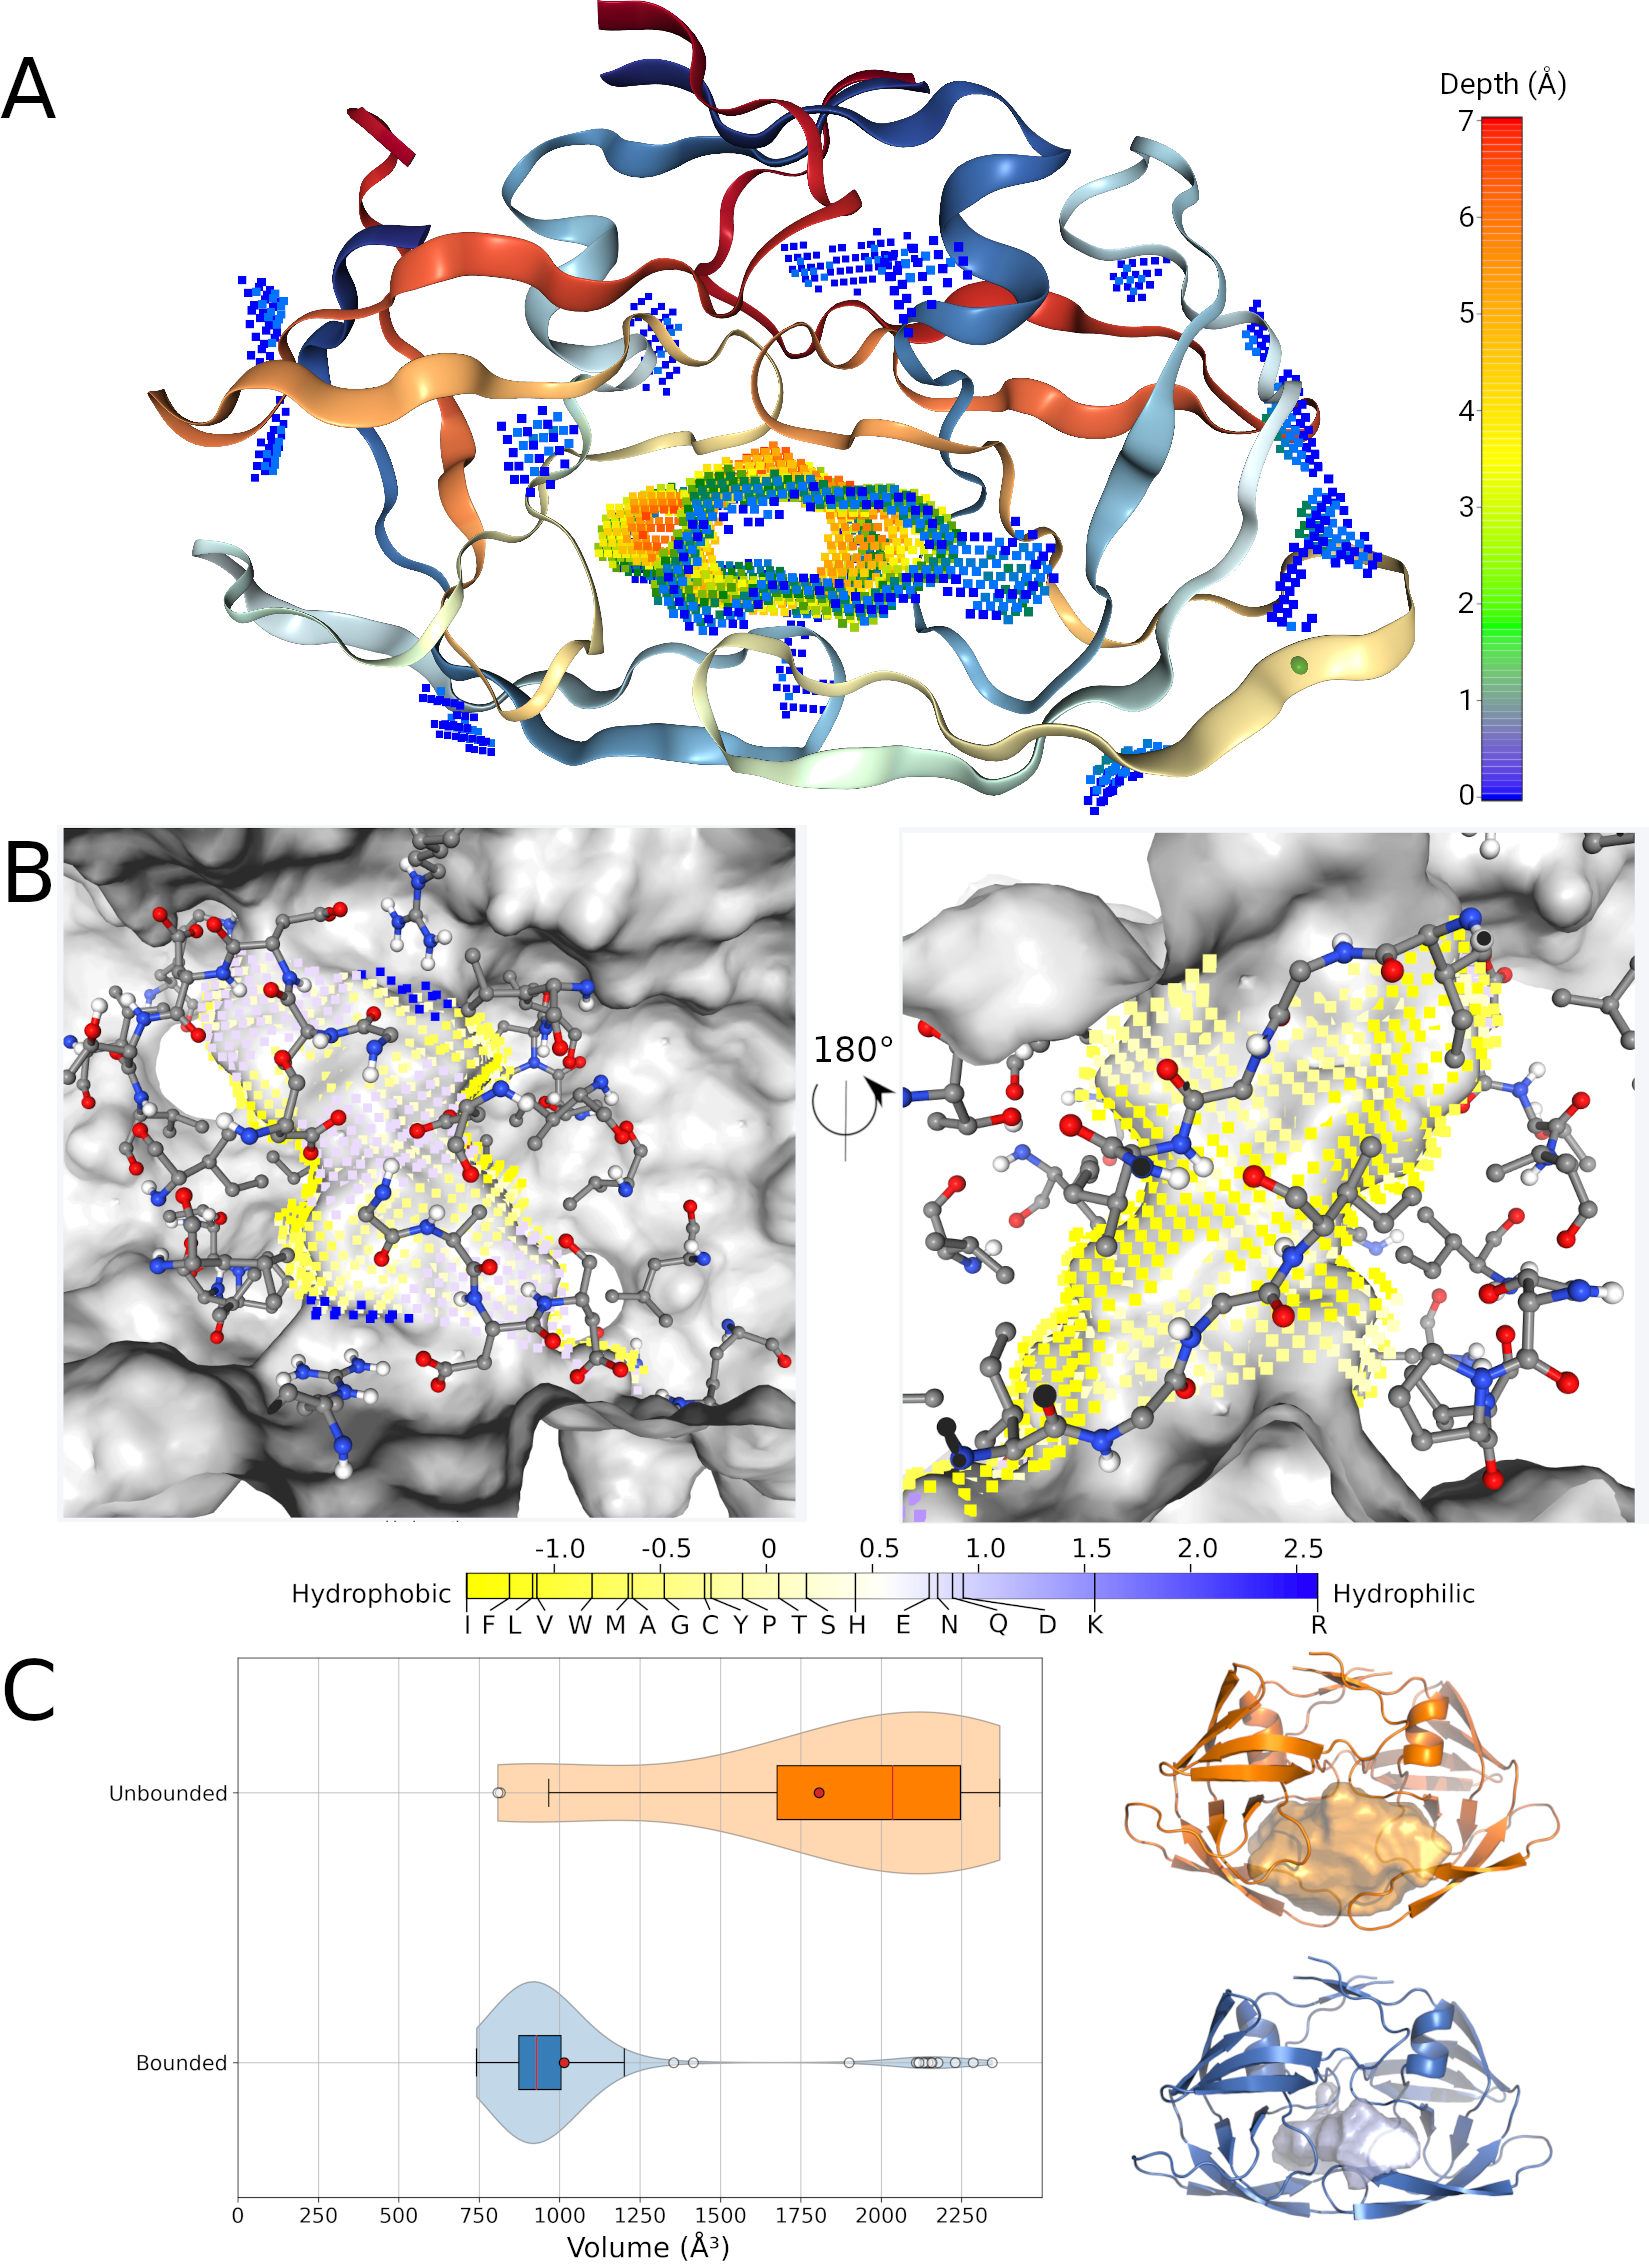
\includegraphics[scale=1.8]{images/kvweb-case-study.png}
  \centerline{\tiny{\textbf{Source:} Reprinted from \cite{guerra2023A}. Licensed under \href{https://creativecommons.org/licenses/by/4.0/}{CC BY 4.0}.}}
  \caption[Illustrative example of cavity detection and characterization in the HIV-1 protease]{\textbf{Illustrative example of cavity detection and characterization in the HIV-1 protease.}  \textbf{(A)} Cavities detected throughout the HIV-1 protease (PDB ID: 1HVR). Cavity points are colored according to depth in a rainbow color scale. \textbf{(B)} Hydropathy mapped on surface cavity points in regions around the catalytic aspartic acids (left panel) and around the \textbeta-hairpins (right panel). The Eisenberg & Weiss hydrophobicity scale ranges from -1.42 (highly hydrophobic) to 2.6 (highly hydrophilic). The protein is shown as a gray surface, and interface residues are shown as colored atoms in sticks. \textbf{(C)} Violin plot of the active site volume of HIV-1 protease structures from the RCSB PDB for structures with ligands bound at the active site (blue) and structures without ligands (orange). Structures with a median volume and the corresponding cavity are shown as a cartoon and surface model, respectively.}
  \label{fig:kvweb-case-study}
\end{figure}

\subsubsection{Morphological Comparison of the Catalytic Site of HIV-1 Protease Structures}

As discussed in Section \ref{sec:md-hiv1-protease}, the \acs{HIV-1} protease is an effective therapeutic target, with its catalytic site being target of various antiretroviral drugs. The catalytic cycle hinges on the movements of the \textbeta-hairpins, controlling the substrate accessibility to the active site \cite{lam1994,soares2016}. Consequently, we conducted a comprehensive analysis of \acs{HIV-1} protease structures available in the \acs{PDB}, comparing their cavities (refer to \cite{guerra2023A}). Thus, cavity volumes proved instrumental in clearly distinguishing ligand-bound and non-ligand-bound structures (Figure \ref{fig:kvweb-case-study}C), indicating geometric complementarity between the receptor and ligands, supported by physicochemical complementarity elucidated by the hydrophobicity profile.

\subsection{Discussion}

The KVFinder-web represents a significant advancement in the field of biomolecular structural and functional characterization, offering a user-friendly and efficient solution for cavity detection and characterization. The KVFinder-web portal, along with the PyMOL KVFinder-web Tools, provides an intuitive and user-friendly interface for users to perform cavity detection and characterization on any biomolecular structure. Both interfaces are designed with careful considerations to prevent overutilization of computational resources, ensuring a smooth and efficient operation of the KVFinder-web service. For users more familiarized with, the PyMOL plugin mirrors the key functionalities of the parKVFinder PyMOL plugin. The KVFinder-web service is a robust and scalable web service, providing a reliable and efficient computational infrastructure for cavity detection and characterization. Together, these components democratize the usage of parKVFinder software within the scientific community (\eg, scientists, educators, and students), eliminating barriers for users who may face challenges in employing computational tools independently.

In essence, KVFinder-web significantly simplifies the process of detecting and characterizing cavities, making it accessible even to less experienced users. Thus far, our data presented $\sim$124 jobs per month since its official release, indicating the adoption and utility of KVFinder-web in the scientific community. The success of KVFinder-web, as evidenced by its monitoring and analytics, highlights its effectiveness in achieving the goals of simplifying cavity analysis and promoting broader engagement within the scientific community.

\section{SERD \label{sec:serd}}

Molecular recognition hinges on the accessibility of a ligand to the binding site of its corresponding receptor. The atoms exposed to the solvent in a target biomolecule represent the potential interaction points for ligands. However, the identification of protein-protein interfaces through conventional methods, such cavity detection, poses a challenge. These interfaces are often large, flat, and featureless, earning the classification of "undruggable". \acsp{PPI} typically involve contiguous epitopes of one partner and a well-defined groove or series of specific small pockets \cite{jubb2012}, requiring the recognition of exposed residues to facilitate a more focused study of interaction hotspots in a target receptor, especially in molecular docking studies (\eg, protein-ligand docking and protein-protein docking).

\begin{figure}[h]
  \centering
  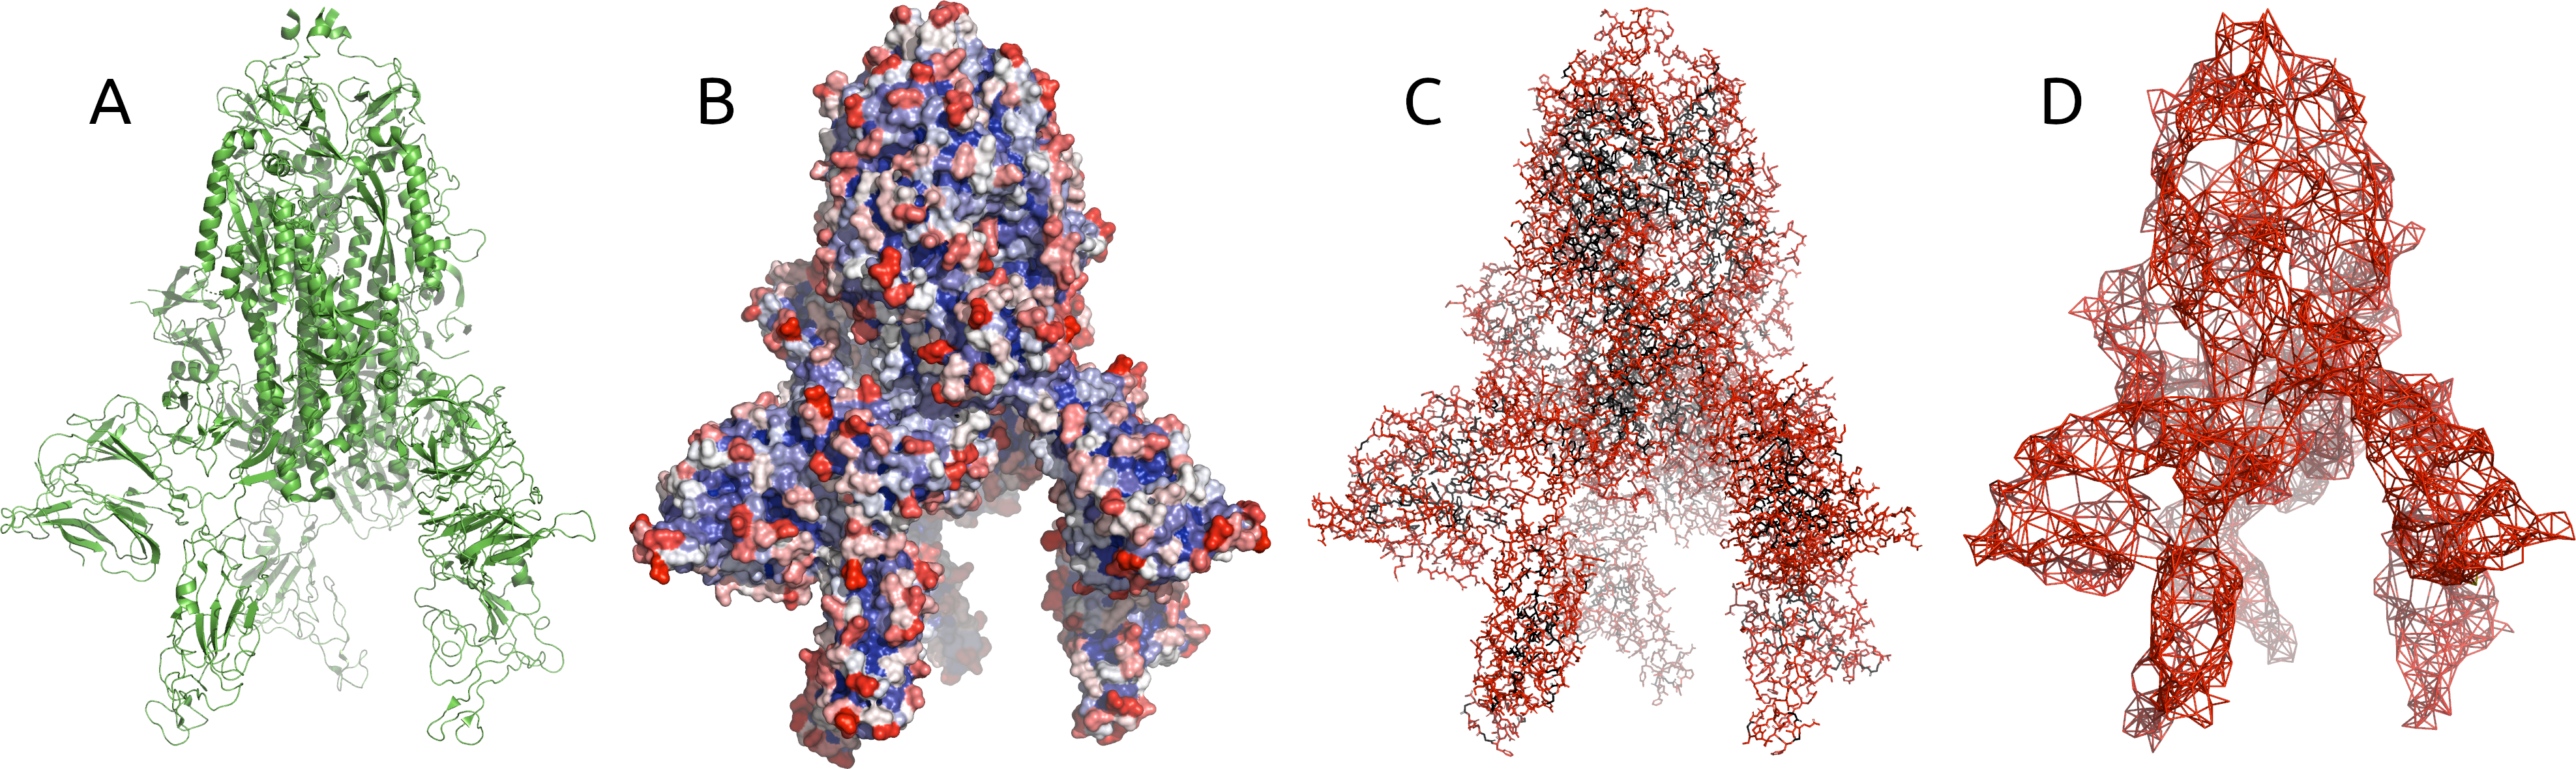
\includegraphics[scale=0.475]{images/serd-spyke.png}
  \caption[Solvent accessibility and graph-based representation in SERD.]{\textbf{Solvent accessibility and graph-based representation in SERD.} \textbf{(A)} SARS-CoV-2 Spike Glycoprotein (PBD ID: 7A98), represented as green cartoon. \textbf{(B)} Solvent accessibility, from low accessibility (blue) to high accessibility (red). \textbf{(C)} Solvent-exposed residues (red sticks). \textbf{(D)} Graph-based representation of solvent-exposed residues. Edges are formed up to the limit distance of 10 Å between \acs{CA} (red).}
  \label{fig:serd-spyke}
\end{figure}

In this scenario, we developed \ac{SERD} \cite{SERD}, an open-source tool licensed under GPL v3.0, designed to detect solvent-exposed residues of a target biomolecule (Figure \ref{fig:serd-spyke}). The algorithm employs a spherical probe, approximating a solvent or ligand molecule, to scan the target biomolecule and identify regions (\ie, residues) accessible to this spherical probe. This process mirrors the 3D grid scanning of the \textit{Probe Out} in parKVFinder (Figure \ref{fig:parkvfinder-schema}). Essentially, the probe size establishes a cutoff for the solvent- or ligand-accessible surfaces (Figure \ref{fig:serd-spyke}B), selectively picking residues beyond this cutoff (Figure \ref{fig:serd-spyke}C).

Transitioning to a broader context, graph theory has been relevant in both biology and pharmaceutical sciences, applied in the study of protein structure, function, and evolution, as well as in \acs{MD} analysis and receptor-ligand interaction networks \cite{vishveshwara2002,mason2007,hummer2023}. As presented in Graphinity \cite{hummer2023}, a graph-based representation of protein-protein complexes, such as antibody-antigen complexes, can be harnessed in deep learning techniques for predicting experimental $\Delta \Delta G$. Moreover, graph-based representations can be employed in a broad range of machine learning techniques and data science applications, as exemplified in Section \ref{sec:graph-representation} and discussed in previous studies \cite{majeed2020,vishveshwara2002,mason2007}. In this context, \acs{SERD} further contributes by representing exposed residues in graph form using the NetworkX library \cite{networkx}. This involves forming edges up to a specified distance between \acs{CA}, \acs{CB}, or any atoms of the residue, optionally including these distances as attributes of the edges of these graphs, as illustrated in Figure \ref{fig:serd-spyke}D.

\begin{figure}[H]
  \centering
  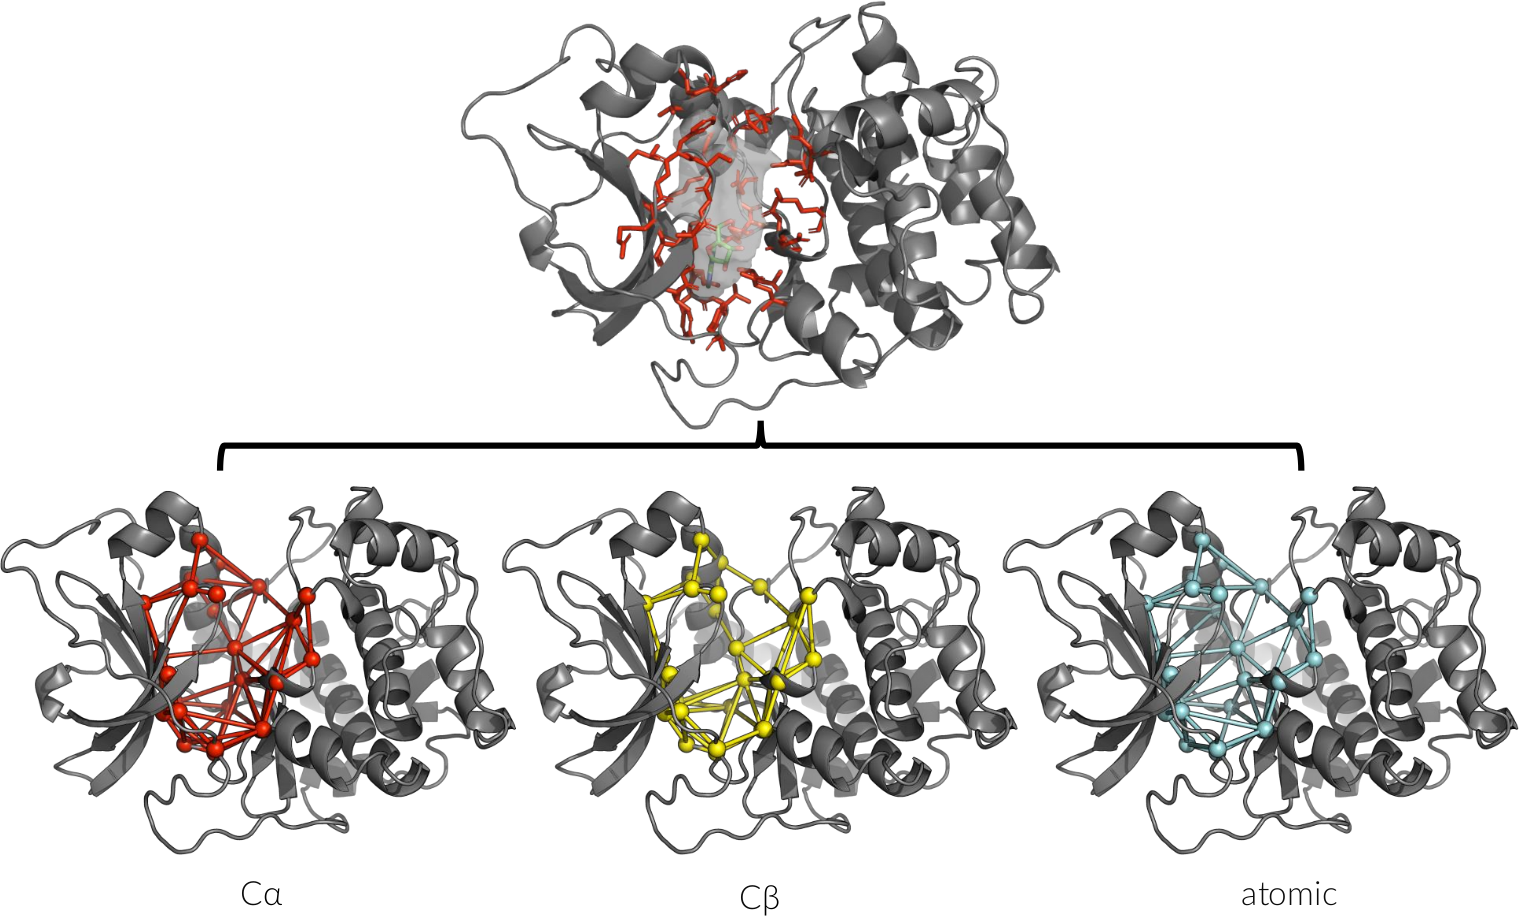
\includegraphics[scale=0.75]{images/graph-representation-of-binding-sites.png}
  \caption[Graph-based representation of the adenosine binding site of protein kinase A.]{\textbf{Graph-based representation of the adenosine binding site of protein kinase A (PDB ID: 1FMO).} Upper panel: Binding site represented in pyKVFinder as a cavity (gray surface) and by the residues surrounding the cavity (red). Lower panel: Binding site represented as graphs. Edges are formed up to the limit distance of 10 Å between \acs{CA} (red), 8 Å between \acs{CB} (yellow), and 5 Å between any atoms of different residues (cyan).}
  \label{fig:serd-cavity}
\end{figure}

Expanding the scope beyond its initial purpose, the graph-based representations developed in SERD find applicability in binding sites detected by pyKVFinder (Figure \ref{fig:serd-cavity}). This topological representation takes into account intramolecular interactions to construct the edges of the graphs, offering novel perspectives for analyzing binding sites in biomolecules using graph theory.

% TODO: Discuss differences between Ca, Cb and atomic distances for forming edges
% Ca: coarser representation ()
% Cb: intermediate representation
% Atomic: finer representation -> less edges, but more computational intensive (more calculations per residue)
% Image: presenting this idea

In summary, SERD can represent biomolecular structures as graphs, from ligand-binding sites (\eg, cavities identified by the KVFinder suite) to biomolecular complexes (\eg, \acs{PPI}, \acs{PLI}, \acs{PRI}, and \acs{PDI}), as shown in Figure \ref{fig:graph-representation}. To date, this tool has been applied in two collaborations at \acs{LBC}: the Master's project of student Marcos Rogério Simões from \acs{PPGCF}/\acs{FCF}, entitled "Description and characterization of binding sites through graph theory", studying the similarity between binding sites among kinase families, and the research project, led by Dr. Gabriel Ernesto Jara, exploring antibody-antigen complexes through surface fragments, represented as graphs. Currently, \acs{SERD} is in version \href{https://github.com/LBC-LNBio/SERD/releases/tag/v0.1.2}{v0.1.2}. The source code is available at the following repository: \url{https://github.com/LBC-LNBio/SERD}.

\section{KVFinderMD}

In specific scenarios, receptors utilize binding sites for the formation of the receptor-ligand complex, which are not easily identified in the unbound form. Certain biomolecular interactions (\eg, \acsp{PPI}, \acs{PLI}, \acs{PRI}, and \acs{PDI}) rely on the intrinsic dynamics of the target receptor, where the classical lock-and-key model fails, and more recent binding models, \eg, induced fit and conformational selection, thrive. In summary, while the lock-and-key model implies a rigid active site, the induced fit model introduces flexibility in both enzyme and substrate, and the conformational selection model highlights the role of pre-existing enzyme conformations that can be selected by substrate binding \cite{holyoak2013} (Figure \ref{fig:molecular-recognition}). In this context, \acs{MD} simulations serve as a useful tool to comprehend molecular recognition process and, ultimately, biomolecular function.

\begin{figure}[h]
  \centering
  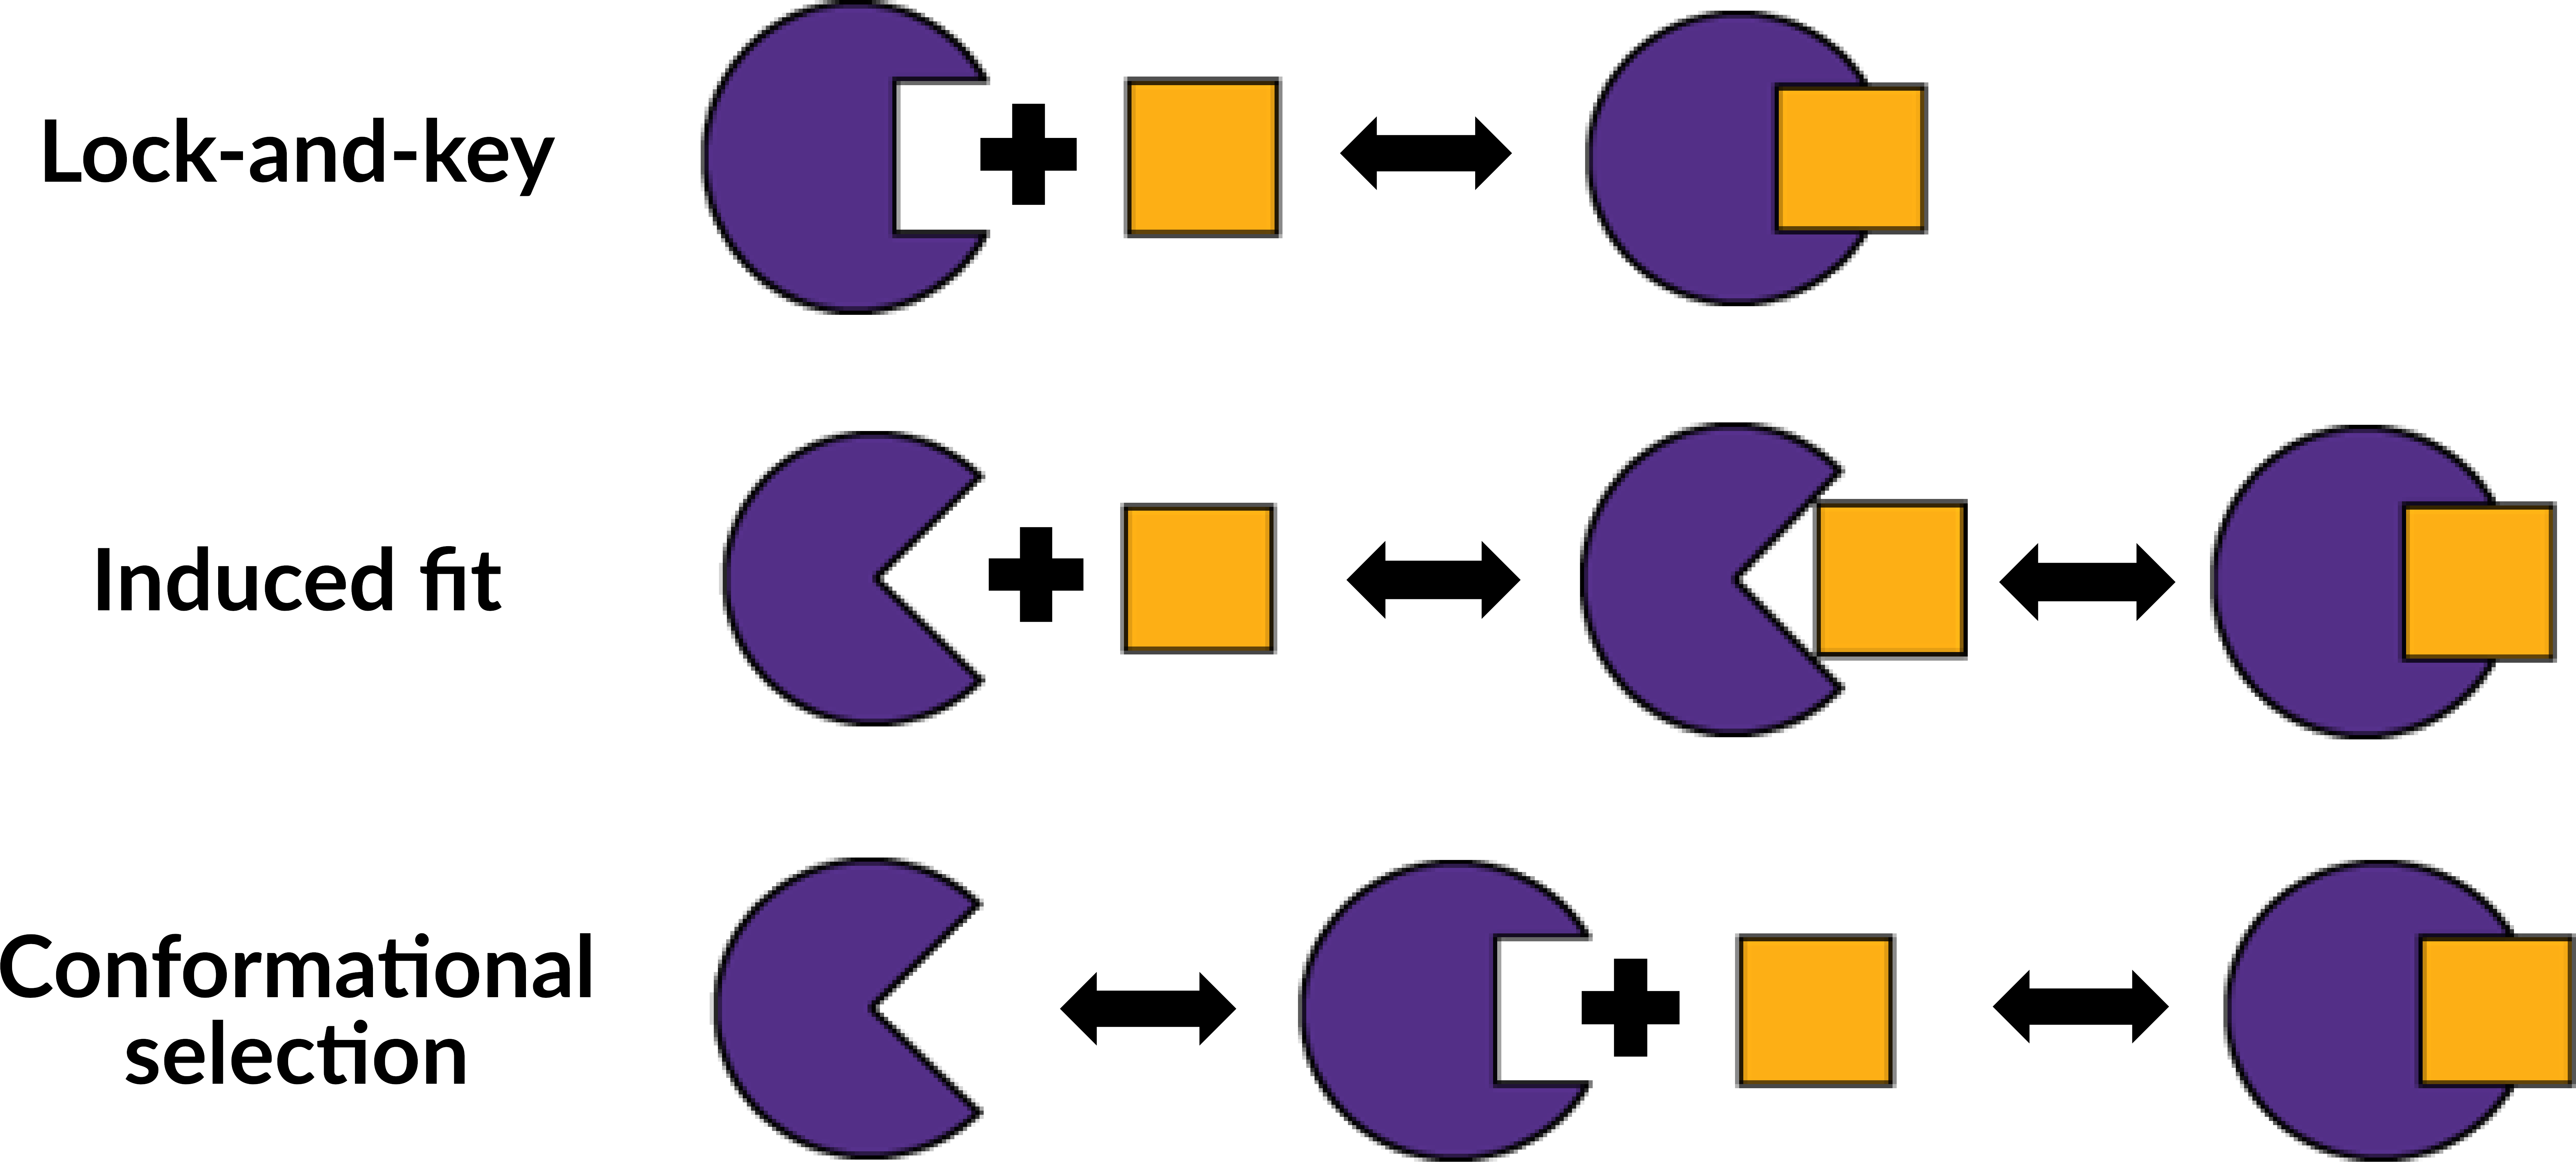
\includegraphics[scale=0.3]{images/molecular-recognition.png}
  \caption[Schematic representation of binding models]{\textbf{Schematic representation of binding models.}}
  \label{fig:molecular-recognition}
\end{figure}

Recently, we developed pyKVFinder \cite{guerra2021} as a foundational element for more complex applications, such as analyses of MD simulations. Building upon it, we developed a new tool, called \ac{KVFinderMD}, a Python package to explore binding site dynamics in biomolecular structures of interest (Figure \ref{fig:kvmd-overview}). For the reading of binary data generated by \acs{MD} simulation programs such as GROMACS \cite{gromacs}, AMBER \cite{amber}, and CafeMol \cite{kenzaki2011}, we employ the MDAnalysis package \cite{mdanalysis} to integrate the reading and processing of \acs{MD} trajectory files (\eg, GRO, CRD, NC, DCD, XTC/TRR) and topology files (\eg, PSF, PRMTOP, GRO, PDB) into KVFinderMD. Given that the intrinsic dynamics of the biomolecule can alter the shape and properties of the binding site over time, KVFinderMD characterizes cavities in respect to volume, area, depth, hydrophobicity, and interface residues---properties crucial for describing the molecular recognition process (Figure \ref{fig:kvmd-overview}A). Additionally, we implemented a protocol for the analysis of cavity conservation throughout MD (Figure \ref{fig:kvmd-overview}A; bottom right panel), similar to the conservation analysis of the ADP-ribose binding site in the \acs{ADRP} domain of \acs{SARS-CoV-2} and related proteins (Figure \ref{fig:conservation-analysis}). Besides that, we also integrated the graph-based representation implemented in SERD (see Sections \ref{sec:graph-representation} and \ref{sec:serd}), considering \acs{CA}, \acs{CB}, or atomic distances, to describe the binding site (Figure \ref{fig:kvmd-overview}B). With it, cavity similarity can be determined by hierarchically clustering different cavity representations available in KVFinderMD (\ie, 3D grid, residue-level representation, and graph-based representation), allowing for tracking cavities throughout \acs{MD} simulation.

\begin{figure}[h]
  \centering
  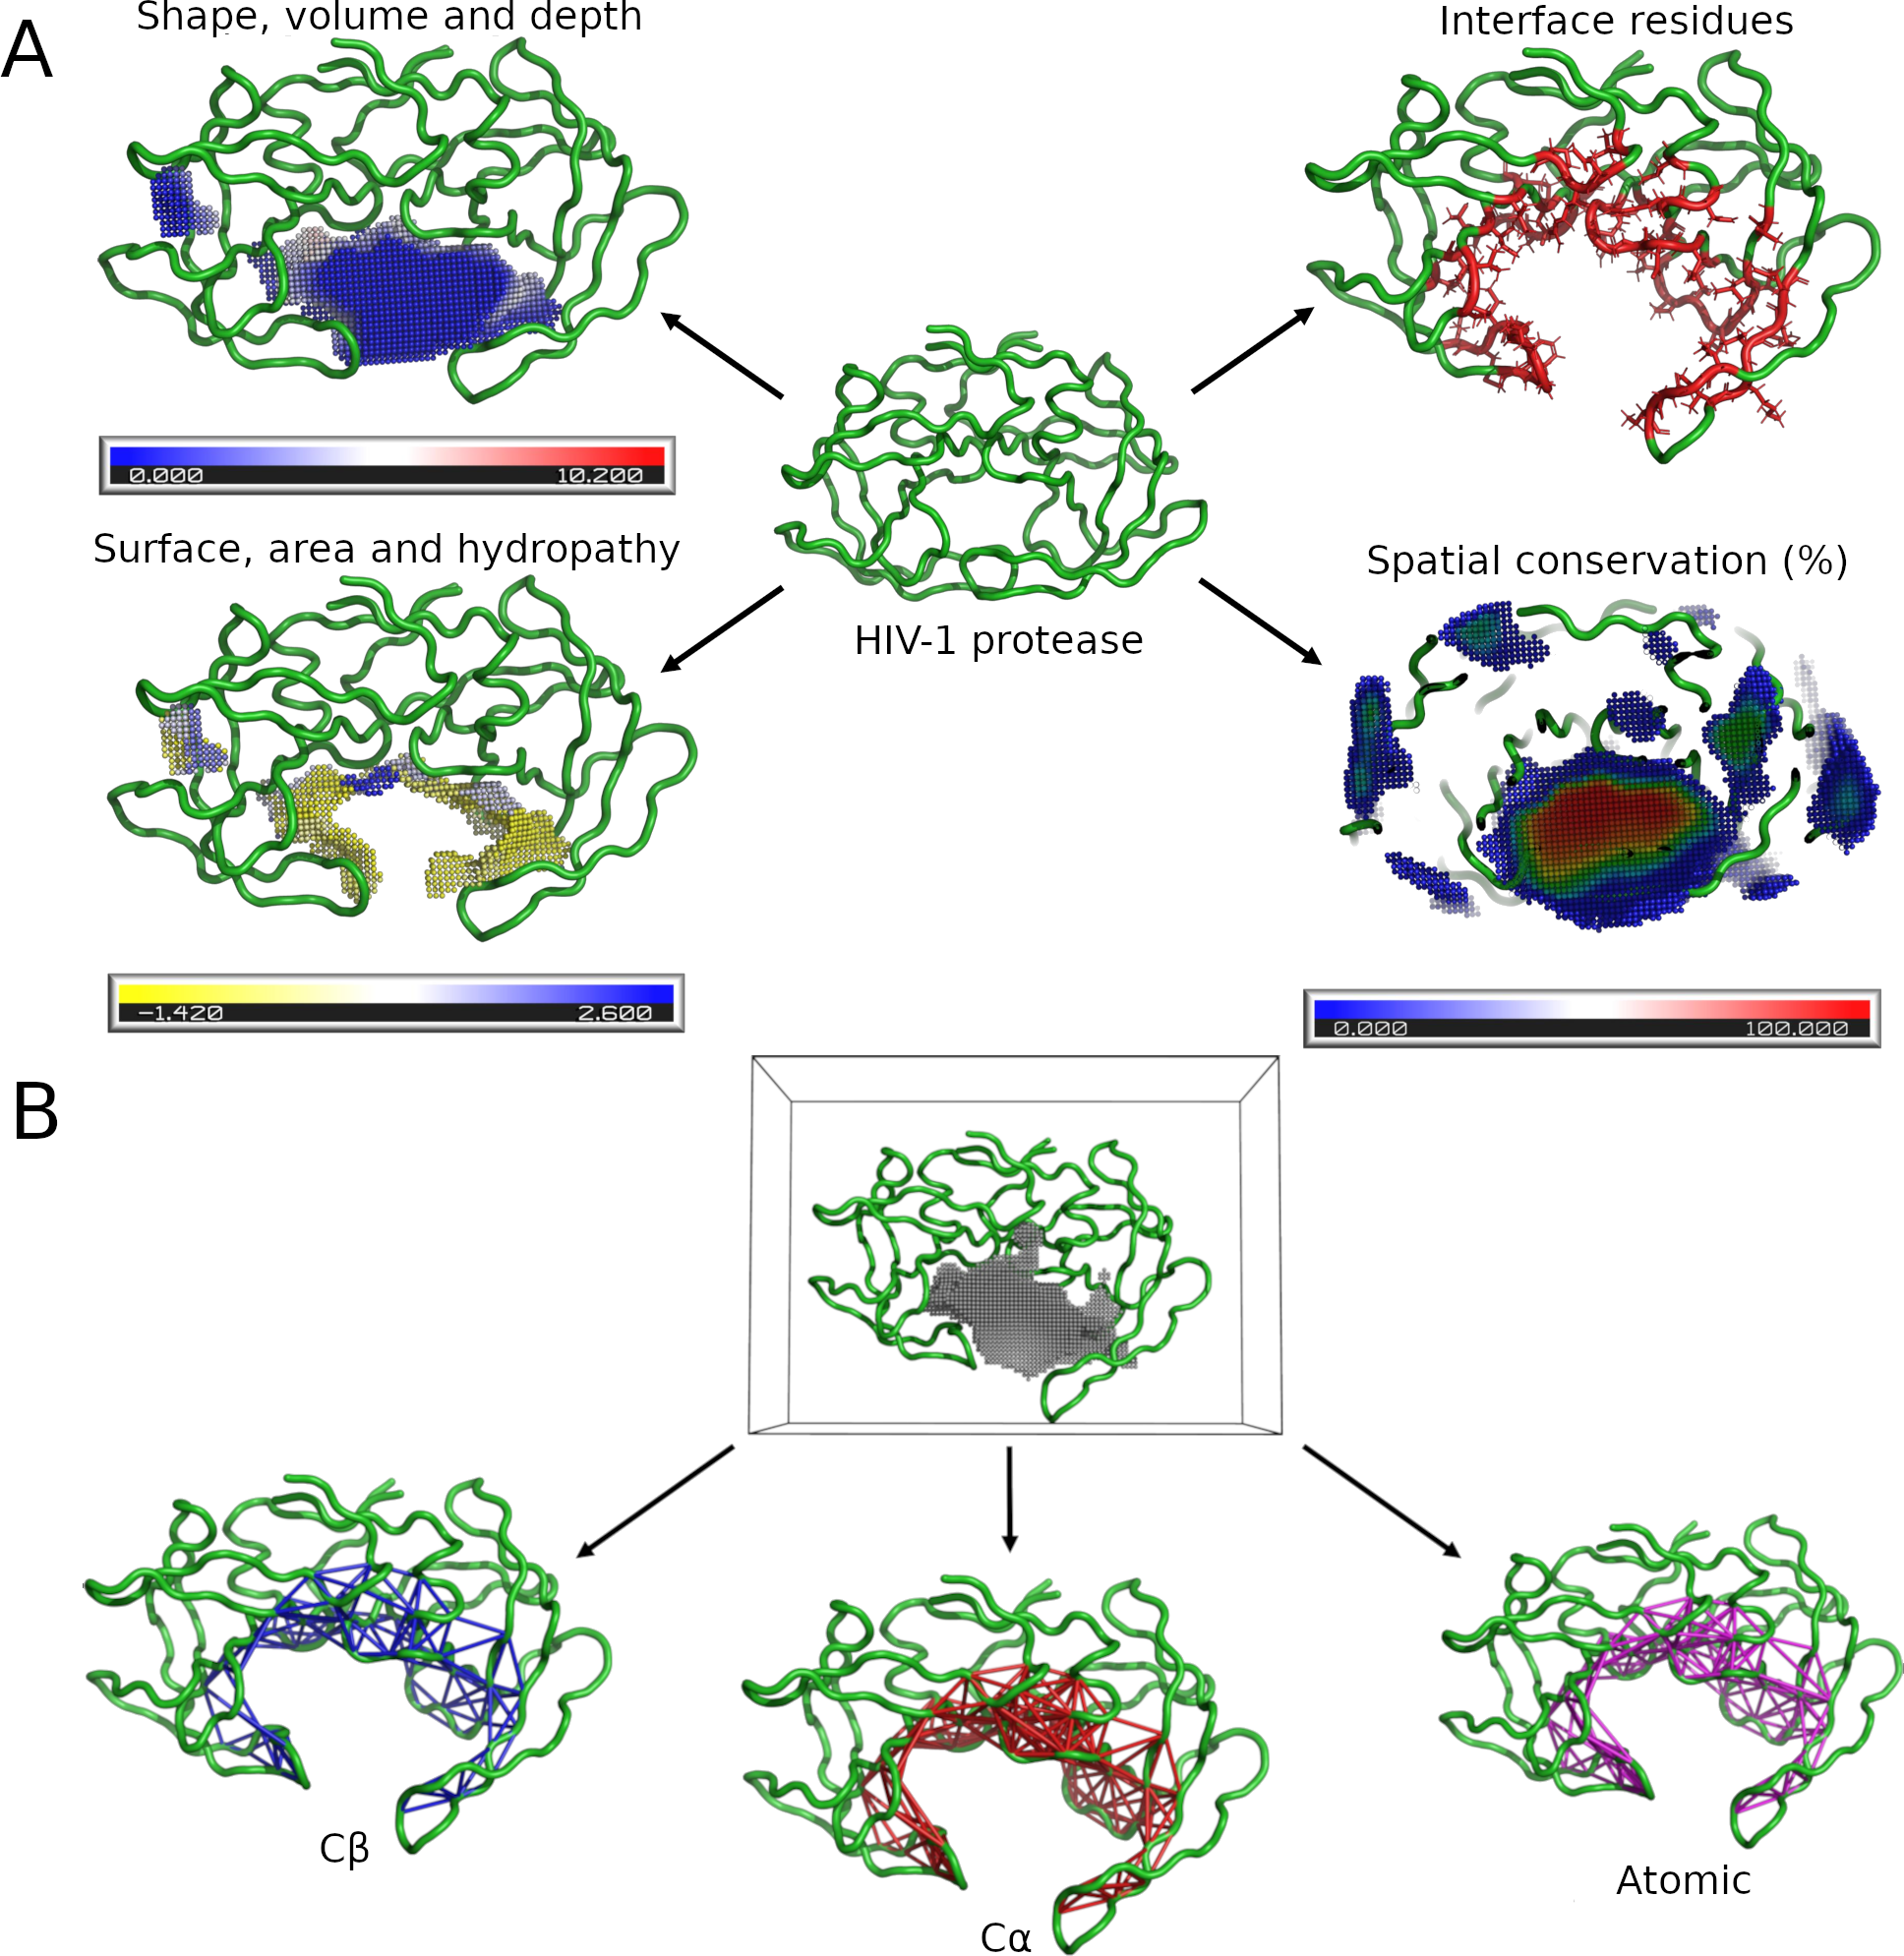
\includegraphics[scale=0.75]{images/kvmd-overview.png}
  \caption[Detection, characterizations, and representations of cavities in molecular dynamics studies using the KVFinderMD tool.]{\textbf{Detection, characterizations, and representations of cavities in molecular dynamics studies using the KVFinderMD tool.} \textbf{(A)} Morphological, topological, and physicochemical characterizations applied in KVFinderMD. \textbf{(B)} Graph-based representation of cavities based on interface residues and their topological relationships. Edges are formed up to the limit distance of  8 Å between \acs{CB} (blue), 10 Å between \acs{CA} (red), and 5 Å between any atoms of different residues (magenta).}
  \label{fig:kvmd-overview}
\end{figure}

\subsection{Case Study}

The KVFinderMD was applied in a case study to explore the cavity similarity of the HIV-1 protease throughout a \acs{MD} simulation. This case study was presented at the \ac{CEC}, held between November 22 and 24, 2022, and received an award for the presentation entitled "KVFinderMD: a Python package to detect and describe binding sites in molecular dynamics trajectories".

\subsubsection{Cavity Similarity of HIV-1 Protease throughout Molecular Dynamics Simulation}

Computational tools for studying \acs{MD} simulations face challenges in defining the continuity of cavities over time, mainly due to shape changes and the merging and splitting of cavities. To address this issue algorithmically, we can calculate cavity similarity through a structural alignment. From the \acs{MD} simulation of the \acs{HIV-1} protease, where we successfully described the conformational dynamics of the active site (see Section \ref{sec:md-hiv1-protease}), we developed a structural cavity alignment methodology to determine cavity similarity throughout a \acs{MD} simulation, using KVFinderMD. The methodology consists of three steps:

\begin{enumerate}
  \item Detection and characterization of cavities in the \acs{HIV-1} protease throughout the entire \acs{MD} simulation using KVFinderMD;
  \item Representation of these cavities in various formats, including 3D grid representation, residue-level representation, and graph-based representation;
  \item Application of hierarchical clustering by KVFinderMD to group cavities based on the similarity of their representations, exploring different affinity metrics.
\end{enumerate} 

In the \acs{MD} simulation of the \acs{HIV-1} protease, we detected 672 cavities over 201 simulation frames, using \textit{Probe Out} of 12 $\AA$ and \textit{Volume Cutoff} of 50 $\AA^3$. Subsequently, each cavity was treated as an independent data structure---represented in a 3D grid, residue-level representation, and graph-based representation (Figure \ref{fig:hiv-1-representation}). The 3D grid represents cavities as a boolean grid of dimensions (160, 126, 105), totaling $2.1 \cdot 10^6$ voxels. Cavity points are assigned with 1, while other points (biomolecule, solvent, and empty space) are marked as 0. For the residue-level representation, cavities are expressed as a square matrix depicting distances between constituent residues. In the graph-based representation, cavities are represented as a square matrix presenting contacts between constituent residues. These contacts are determined by the distance between the \acs{CB} atoms of residues, employing a distance cutoff of 8 $\AA$, the default metric of SERD. Both square matrices are ordered according to the protein sequence with 198 aminoacids, totalizing $3.9 \cdot 10^4$ points.

\begin{figure}[h]
  \centering
  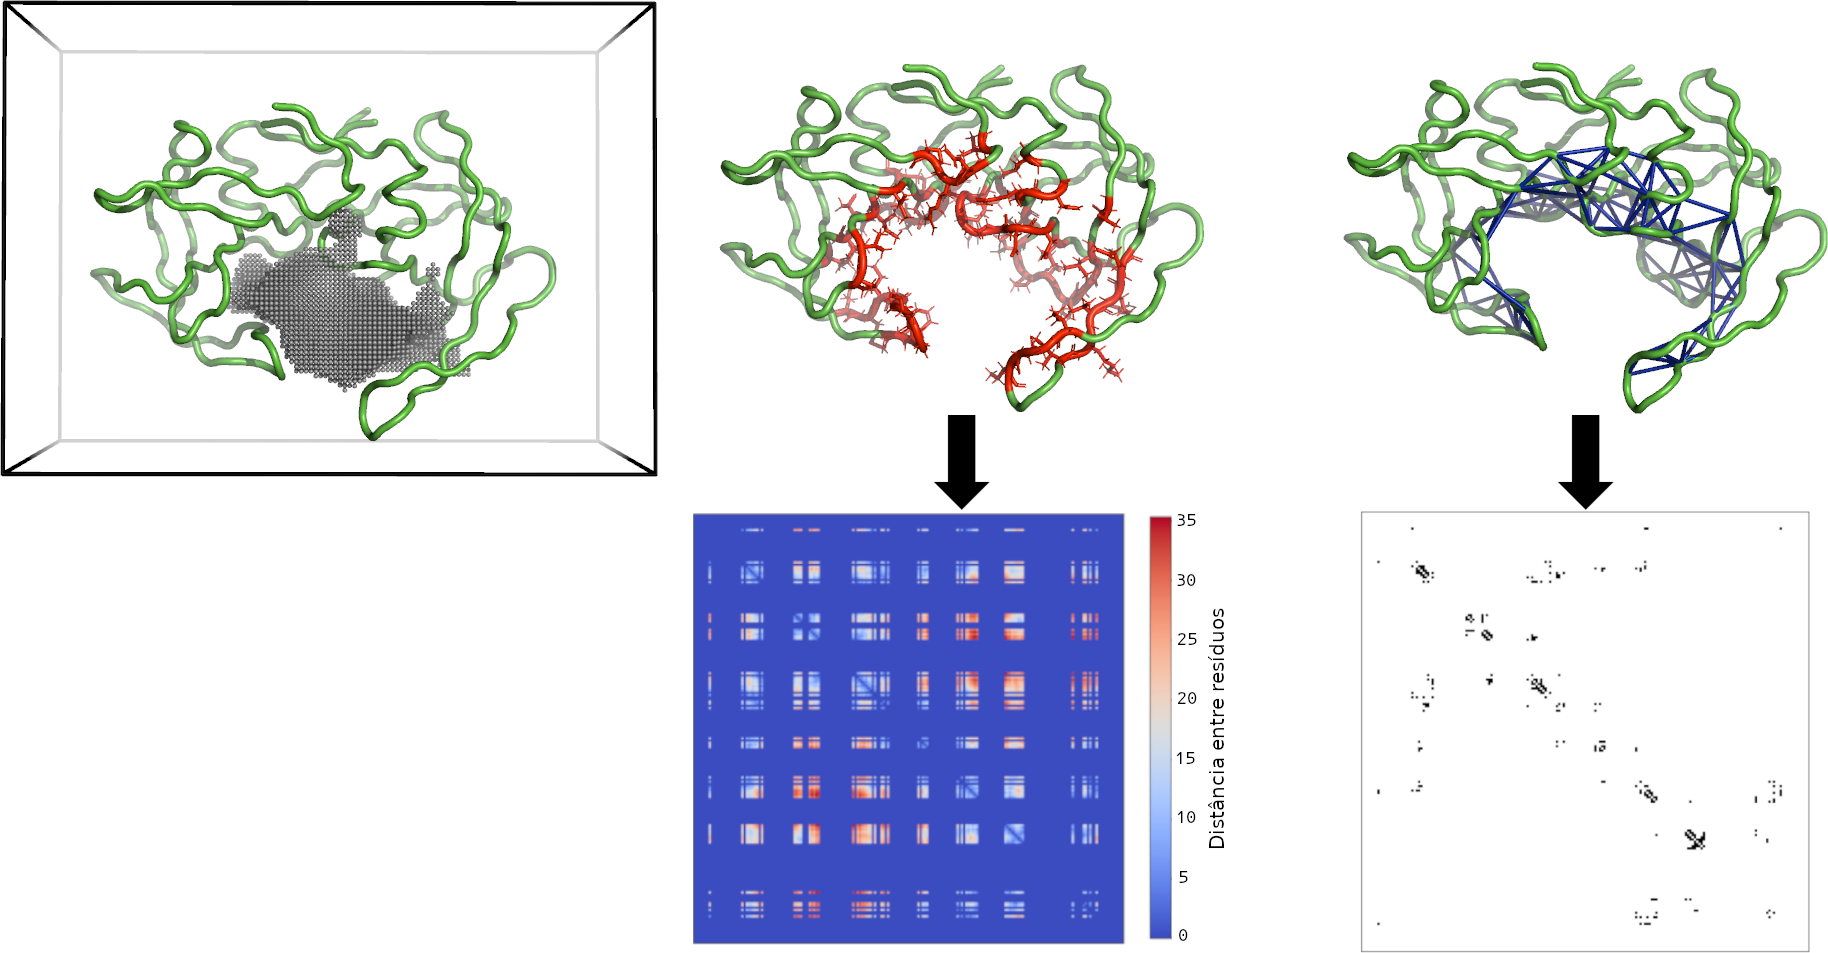
\includegraphics[scale=1]{images/HIV-1-representation.png}
  \caption[Cavity representation for the study of HIV-1 protease cavity similarity throughtout molecular dynamics trajectory]{\textbf{Cavity representation for the study of HIV-1 protease cavity similarity throughtout molecular dynamics trajectory.} Representation of the active site cavity in 3D grid (left panel), where cavity points are identified by 1, while other points (biomolecule points, solvent points, and empty space points) are identified by the value 0. Residue-level representation of the active site (central panel), where we abstract cavities as a distance matrix between \acs{CB} atoms of residues, ordered by the protein sequence. Graph-based representation of relationships between active site residues (right panel), where we abstract cavities as a contact matrix, ordered by the protein sequence.}
  \label{fig:hiv-1-representation}
\end{figure}

With these cavity representations, clustering analysis groups them based on their similarity. Hierarchical clustering, compared to other unsupervised clustering methods, yield more interpretable results, by providing a similarity relationship between cavity representations. As there is no ground truth for an unlabeled cluster analysis (\ie, structural cavity alignment), the silhouette score ($s$; Eq. \ref{eq:silhouette}), proposed by Peter Rousseeuw \cite{rousseeuw1987}, was used to evaluate the quality of the clustering. This metric measures the similarity of a cavity to its own group (cohesion) compared to other groups (separation), based on an affinity metric. Thus, achieving a silhouette score of 1 is optimal for cluster validity, while a score of -1 signifies poor clustering, and 0 implies clusters with overlapping boundaries.

\begin{equation}
  s \colon (i) \mapsto \frac{(b(i) - a(i))}{max(a(i), b(i))} \in [-1, 1]
  \label{eq:silhouette}
\end{equation}

\noindent where $a$ is the mean intra-cluster distance, $b$ is the mean nearest-cluster distance, and $i$ is a given cavity.

In simpler terms, 672 data structures (\ie, cavities) are clustered by hierarchical clustering, exploring appropriate affinity metrics for each cavity representation. Since the silhouette score cannot be compared between different affinity metrics, we compared affinity metrics based on the ideal number of clusters by maximizing the mean silhouette score over all cavity representations (Eq. \ref{eq:silhouette-coefficient}), as proposed by Leonard Kaufmann and Peter Rousseeuw \cite{kaufman1990}.

\begin{equation}
  k \mapsto \argmax_k \tilde{s}(k) \in [2,\infty)
  \label{eq:silhouette-coefficient}
\end{equation}

\noindent where $\tilde{s}(k)$ represents the mean $s(i)$ over all cavities of the \acs{MD} simulation for a specific number of clusters $k$.

For non-negative real-valued vectors, we evaluated the following metrics available in the SciPy package \cite{scipy}: correlation distance ($\rho$; Eq. \ref{eq:correlation}), Bray-Curtis distance, Canberra distance, Chebyshev distance, Manhattan distance (also known as City Block distance), cosine distance ($d_{\sf cosine}$; Eq. \ref{eq:cosine}), Jensen-Shannon distance, and squared Euclidean distance. For boolean vectors, we evaluated the following metrics available in the SciPy package \cite{scipy}: Dice dissimilarity ($d_{\sf dice}$; Eq. \ref{eq:dice}), Hamming distance, Jaccard-Needham dissimilarity, Kulczynski dissimilarity, Rogers-Tanimoto dissimilarity, Russell-Rao dissimilarity, Sokal-Michener dissimilarity, Sokal-Sneath dissimilarity, and Yule dissimilarity.

\begin{equation}
  \rho \colon (u,v) \mapsto 1 - \frac{(u - \bar{u}) \cdot (v - \bar{v})}{{\|(u - \bar{u})\|}_2 {\|(v - \bar{v})\|}_2} \in [-1, 1]
  \label{eq:correlation}
\end{equation}

\noindent where $\bar{u}$ is the mean of elements in $u$, $\bar{v}$ is the mean of elements in $v$, and $x \cdot y$ is the dot product of $x$ and $y$.

\begin{equation}
  d_{\sf cosine} \colon (u,v) \mapsto 1 - \frac{u \cdot v}{\|u\|_2 \|v\|_2} \in [-1, 1]
  \label{eq:cosine}
\end{equation}

\noindent where $u \cdot v$ is the dot product of $u$ and $v$.

\begin{equation}
  d_{\sf dice} \colon (u,v) \mapsto \frac{C_{VF}(u,v) + C_{FV}(u,v)}{2 C_{VV}(u,v) + C_{VF}(u,v) + C_{FV}(u,v)} \in [0,1]
  \label{eq:dice}
\end{equation}

\noindent where $C_{ij}$ is the number of occurrences of $u[k] = i$ and $v[k] = j$ for $k<n$.

Following this methodology for structural cavity alignment, cavities are grouped by hierarchical clustering, using the complete linkage method, optimizing the mean silhouette score to find the ideal number of clusters for each affinity metric. Then, the clustered cavities and their respective silhouettes scores of the affinity metrics with the highest number of clusters, for each cavity representation, are presented in Figure \ref{fig:hiv-1-clustering-results}. The structural cavity alignment results are summarized in Table \ref{tab:hiv-1-clustering-summary}. 

\begin{table}[h]
  \caption[Summary of structural cavity analysis in the molecular dynamics simulation of the HIV-1 protease]{\textbf{Summary of structural cavity analysis in the molecular dynamics simulation of the HIV-1 protease.}}
  \centering
  \begin{tabular}{ccccl}
    \cline{1-4}
     &
      \textbf{\begin{tabular}[c]{@{}c@{}}3D grid\\ aligment\end{tabular}} &
      \textbf{\begin{tabular}[c]{@{}c@{}}Distance matrix\\ alignment\end{tabular}} &
      \textbf{\begin{tabular}[c]{@{}c@{}}Contact matrix\\ alignment\end{tabular}} &
       \\ \cline{1-4}
      \textbf{Clusters}  & 10                  & 15                  & 16                  &  \\
      \textbf{Data size} & $\sim$$10^6$/cavity & $\sim$$10^4$/cavity & $\sim$$10^4$/cavity &  \\
      \textbf{Data type} & Boolean (4-bit)     & Float (32-bit)      & Boolean (4-bit)     &  \\ \cline{1-4}
  \end{tabular}
  \label{tab:hiv-1-clustering-summary}
\end{table}

The hierarchical clustering of the 3D grid representation resulted in 10 groups with a mean silhouette score of $\sim$0.42. Due to data size ($\sim$$10^6$ points per cavity), we did not explore different affinity metrics, and therefore, we only used correlation distance (Eq. \ref{eq:correlation}). For the residue-level representation, we explored different affinity metrics, and cosine distance (Eq. \ref{eq:cosine}) showed the highest number of groups among non-negative real-valued metrics (\ie, 15 groups) with a mean silhouette score of $\sim$0.54. For the graph-based representation representation, we explored different affinity metrics, and Dice dissimilarity (Eq. \ref{eq:dice}) showed the highest number of groups among boolean metrics (\ie, 16 groups) with a mean silhouette score of $\sim$0.52.

\begin{figure}[h]
  \centering
  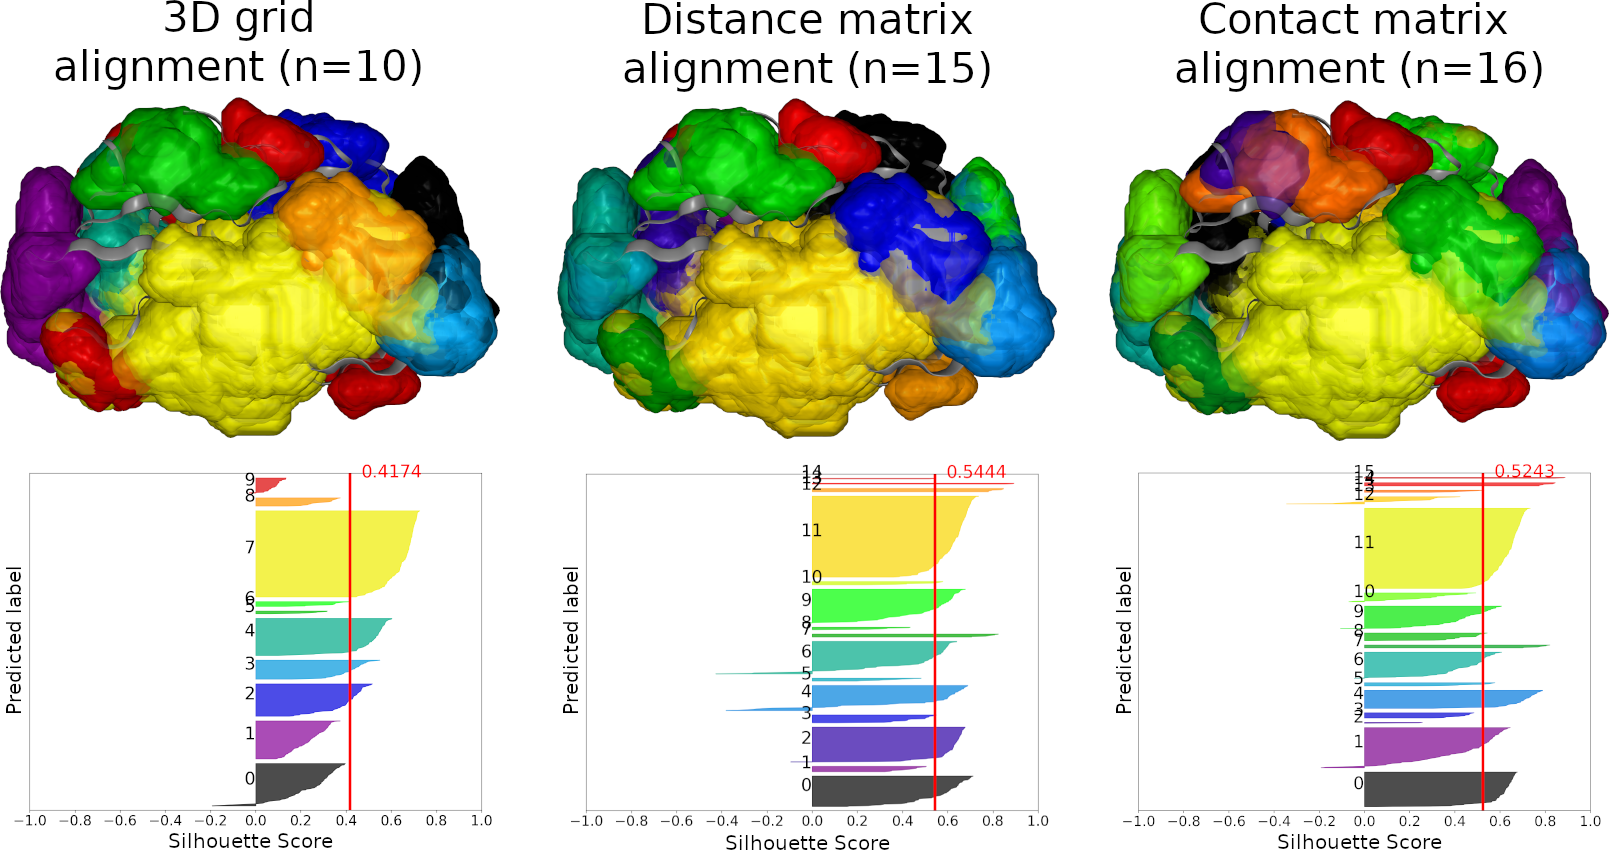
\includegraphics[scale=1]{images/HIV-1-clustering-results.png}
  \caption[Hierarchical clustering of HIV-1 protease cavities]{\textbf{Hierarchical clustering of HIV-1 protease cavities.} All cavities detected throughout the molecular dynamics were overlaid on the same structure and colored according to labels assigned by hierarchical clustering of 3D grid (left panel), distance matrix (central panel), and contact matrix (right panel). The silhouette score plot is presented for each sample according to the assigned label. The red line indicates the silhouette coefficient for hierarchical clustering.}
  \label{fig:hiv-1-clustering-results}
\end{figure}

Furthermore, the data size of the cavity representations highly influences the time complexity of the hierarchical clustering, which is $\mathcal{O}(n^3)$, where $n$ represents the number of points. Thus, the 3D grid is the most computationally intensive ($\sim$$10^6$ points per cavity), followed by the residue-level representation ($\sim$$10^4$ points per cavity) and the graph-based representation ($\sim$$10^4$ points per cavity). With data size simplification for the latter two representations, it was possible to explore different affinity metrics. Basically, the data size decreases by 100 times per cavity compared to the 3D grid structure. Therefore, considering we have 672 cavities in this case study, the size reduction is approximately 67,200 times. Conversely, the data type used by each cavity representation influences the memory usage for the structural cavity alignment. The 3D grid representation uses boolean (8-bit), while the residue-level representation uses float (32-bit floating-point) and the graph-based representation use boolean (8-bit). Thus, the graph-based representation uses less memory than the other representations, with a smaller data size. In summary, the 3D grid representation is the most computationally intensive, followed by the residue-level representation and the graph-based representation. 

In summary, we successfully grouped cavities and tracked their continuity throughout the \acs{MD} simulation, which simplified the comparison of characteristics between cavities over time. The use of distance matrices and contact matrices proved effective due to their ability to cluster cavities. Moreover, these representations were faster and simpler for clustering cavities over time in MD simulations since the hierarchical clustering algorithm has a time complexity of approximately $\mathcal{O}(n^3)$, and the data size decreases by 100 times per cavity compared to the original structure (\ie, 3D grid).

\subsection{Discussion}

The application of KVFinderMD illustrates the integration of tools within the KVFinder suite (\ie, pyKVFinder and SERD) to conduct a systematic analysis of cavities through an automated protocol. By employing hierarchical clustering algorithms and different affinity metrics across various representations (\ie, 3D grid, residue-level representation, and graph-based representation), we identified clusters of similar cavities, enabling the assessment of the temporal evolution of binding sites (\ie, cavity continuity). Additionally, we managed to reduce the data size required for analysis and simplify the comparison between cavities in \acs{MD} simulations, showcasing the practical applicability of the KVFinder suite.

The analysis of cavity similarity in the \acs{HIV-1} protease throughout the \acs{MD} simulation allowed us to track the evolution of these cavities and compare their characteristics over time, as depicted in Figure \ref{fig:hiv1-protease-dm-analysis}. This was achieved without human intervention, utilizing the automated features of KVFinderMD. However, it is important to note that, while KVFinderMD is a valuable tool for cavity analysis in \acs{MD} simulations, there are some limitations to consider. For instance, the choice of affinity metrics and hierarchical clustering parameters can influence the obtained results. Therefore, careful evaluation and exploration of different configurations are essential for optimal outcomes.

Despite these limitations, KVFinderMD represents a significant advancement in the study of biomolecular interactions over time. ts ability to automate cavity analysis in \acs{MD} simulations, coupled with other tools in the KVFinder suite, provides a comprehensive approach to investigate binding sites and understand their evolution. This can be valuable in the development of therapeutic strategies and the rational design of new drugs, especially in transient binding sites.

\section{Benchmarking of Well-established Cavity Detection Tools}

Cavity detection methods are usually only benchmarked on their ability to detect binding sites (\ie, qualitative assessment), and not on their ability to accurately characterize their volume (\ie, quantitative assessment). Quantitative descriptors still remains a challenge in the cavity detection field, because the "real" cavity volume in biological systems is not experimentally measurable. In collaboration with Dr. György Szalóki (Laboratoire Hétérochimie Fondamentale et Appliquée - Université Toulouse III Paul Sabatier - France), we developed a benchmarking protocol to evaluate the performance of cavity detection tools in a dataset of well-defined artificial supramolecular cages. The source code for the benchmarking protocol (\href{https://github.com/LBC-LNBio/SMC-Benchmarking/releases/tag/v1.0.0}{v1.0.0}) is available at the following repository: \url{https://github.com/LBC-LNBio/SMC-Benchmarking}.

The "real" cavity volume could be derived from the Rebek's rule of thumb \cite{mecozzi1998}, that states, in any biological or artificial host-guest system, the ratio of the guest and host's cavity is $0.55\pm0.09$, termed as packing  coefficient ($PC$; Eq. \ref{eq:packing-coefficient}), when guest encapsulation is only driven by weak intermolecular interactions (\eg, Keesom forces, Debye forces, and London dispersion forces). However, this rule of thumb is not applicable to systems with strong intermolecular forces (\eg, hydrogen bonds), where the packing coefficient can reach up to $0.70$. 

\begin{equation}
  PC \colon (V_{guest},V_{cavity}) \mapsto \frac{V_{guest}}{V_{cavity}} \in [0,1]
  \label{eq:packing-coefficient}
\end{equation}

\noindent where $PC$ is the packing coefficient, $V_{guest}$ is the guest \acs{vdW} volume, and $V_{cavity}$ is the host's cavity volume.

Within this context, there are no existing benchmark dataset to test the performance of cavity characterization methods. Thus, two benchmark datasets, comprising 22 well-known supramolecular cages from the \ac{CSD} \cite{csd}, have been selected from the supramolecular chemistry literature to evaluate the well-established cavity detection tools (see Section \ref{sec:computational-tools}). Since topology and morphology of supramolecular cages differ from biomolecules, cavity detection parameters of the well-established tools (\ie, KVFinder suite, Fpocket, GHECOM and CAVER tools) had to be optimized for the supramolecular cages in both benchmark datasets. The benchmark datasets, Benchmark dataset 1 and Benchmark dataset 2, used in this study, which include the structural data files of each supramolecular cage and guest, are available at Zenodo: \url{https://doi.org/10.5281/zenodo.7702311}.

\subsection{Benchmarking Dataset 1}

The benchmark dataset 1 (Figure \ref{fig:benchmark-dataset-1}) comprises 13 X-ray structures of well-known supramolecular cages, with guest molecules being encapsulated in their void or void-like cavities, following the Rebek's rule of thumb. The guests molecules were removed from their cages and their \acs{vdW} volumes were estimated using \textit{volume} method from \textit{pyKVFinder.Molecule} class (see Section \ref{sec:molecular-volume-estimation}). With it, the "real" cavity volume were calculated using the Rebek's rule of thumb. Then, the cavities of the supramolecular cages were detected and their volumes estimated for each cavity detection tool. As good prediction metrics, the relative error (\acs{RE}; Eq. \ref{eq:re}) and the mean relative absolute error (\acs{MRAE}; Eq. \ref{eq:mrae}) were calculated between cavity volumes.

\begin{equation}
  RE \colon (V,\hat{V}) \mapsto \frac{\hat{V} - V}{V} \in [-\infty,\infty]
  \label{eq:re}
\end{equation}

\noindent where $RE$ is the relative error, $V$ is the "real" cavity volume, and $\hat{V}$ is the estimated cavity volume.

\begin{equation}
  MRAE \colon (V,\hat{V},i) \frac{1}{N_c} \sum_{i=1}^{N_c} \left| \frac{\hat{V_i} - V_i}{V_i} \right| \in [0,\infty]
  \label{eq:mrae}
\end{equation}

\noindent where $MRAE$ is the mean relative absolute error, $V_i$ is the "real" volume of cavity $i$, $\hat{V_i}$ is the estimated volume of cavity $i$, and $N_c$ is the number of cavities.

\begin{figure}[ht]
  \centerline{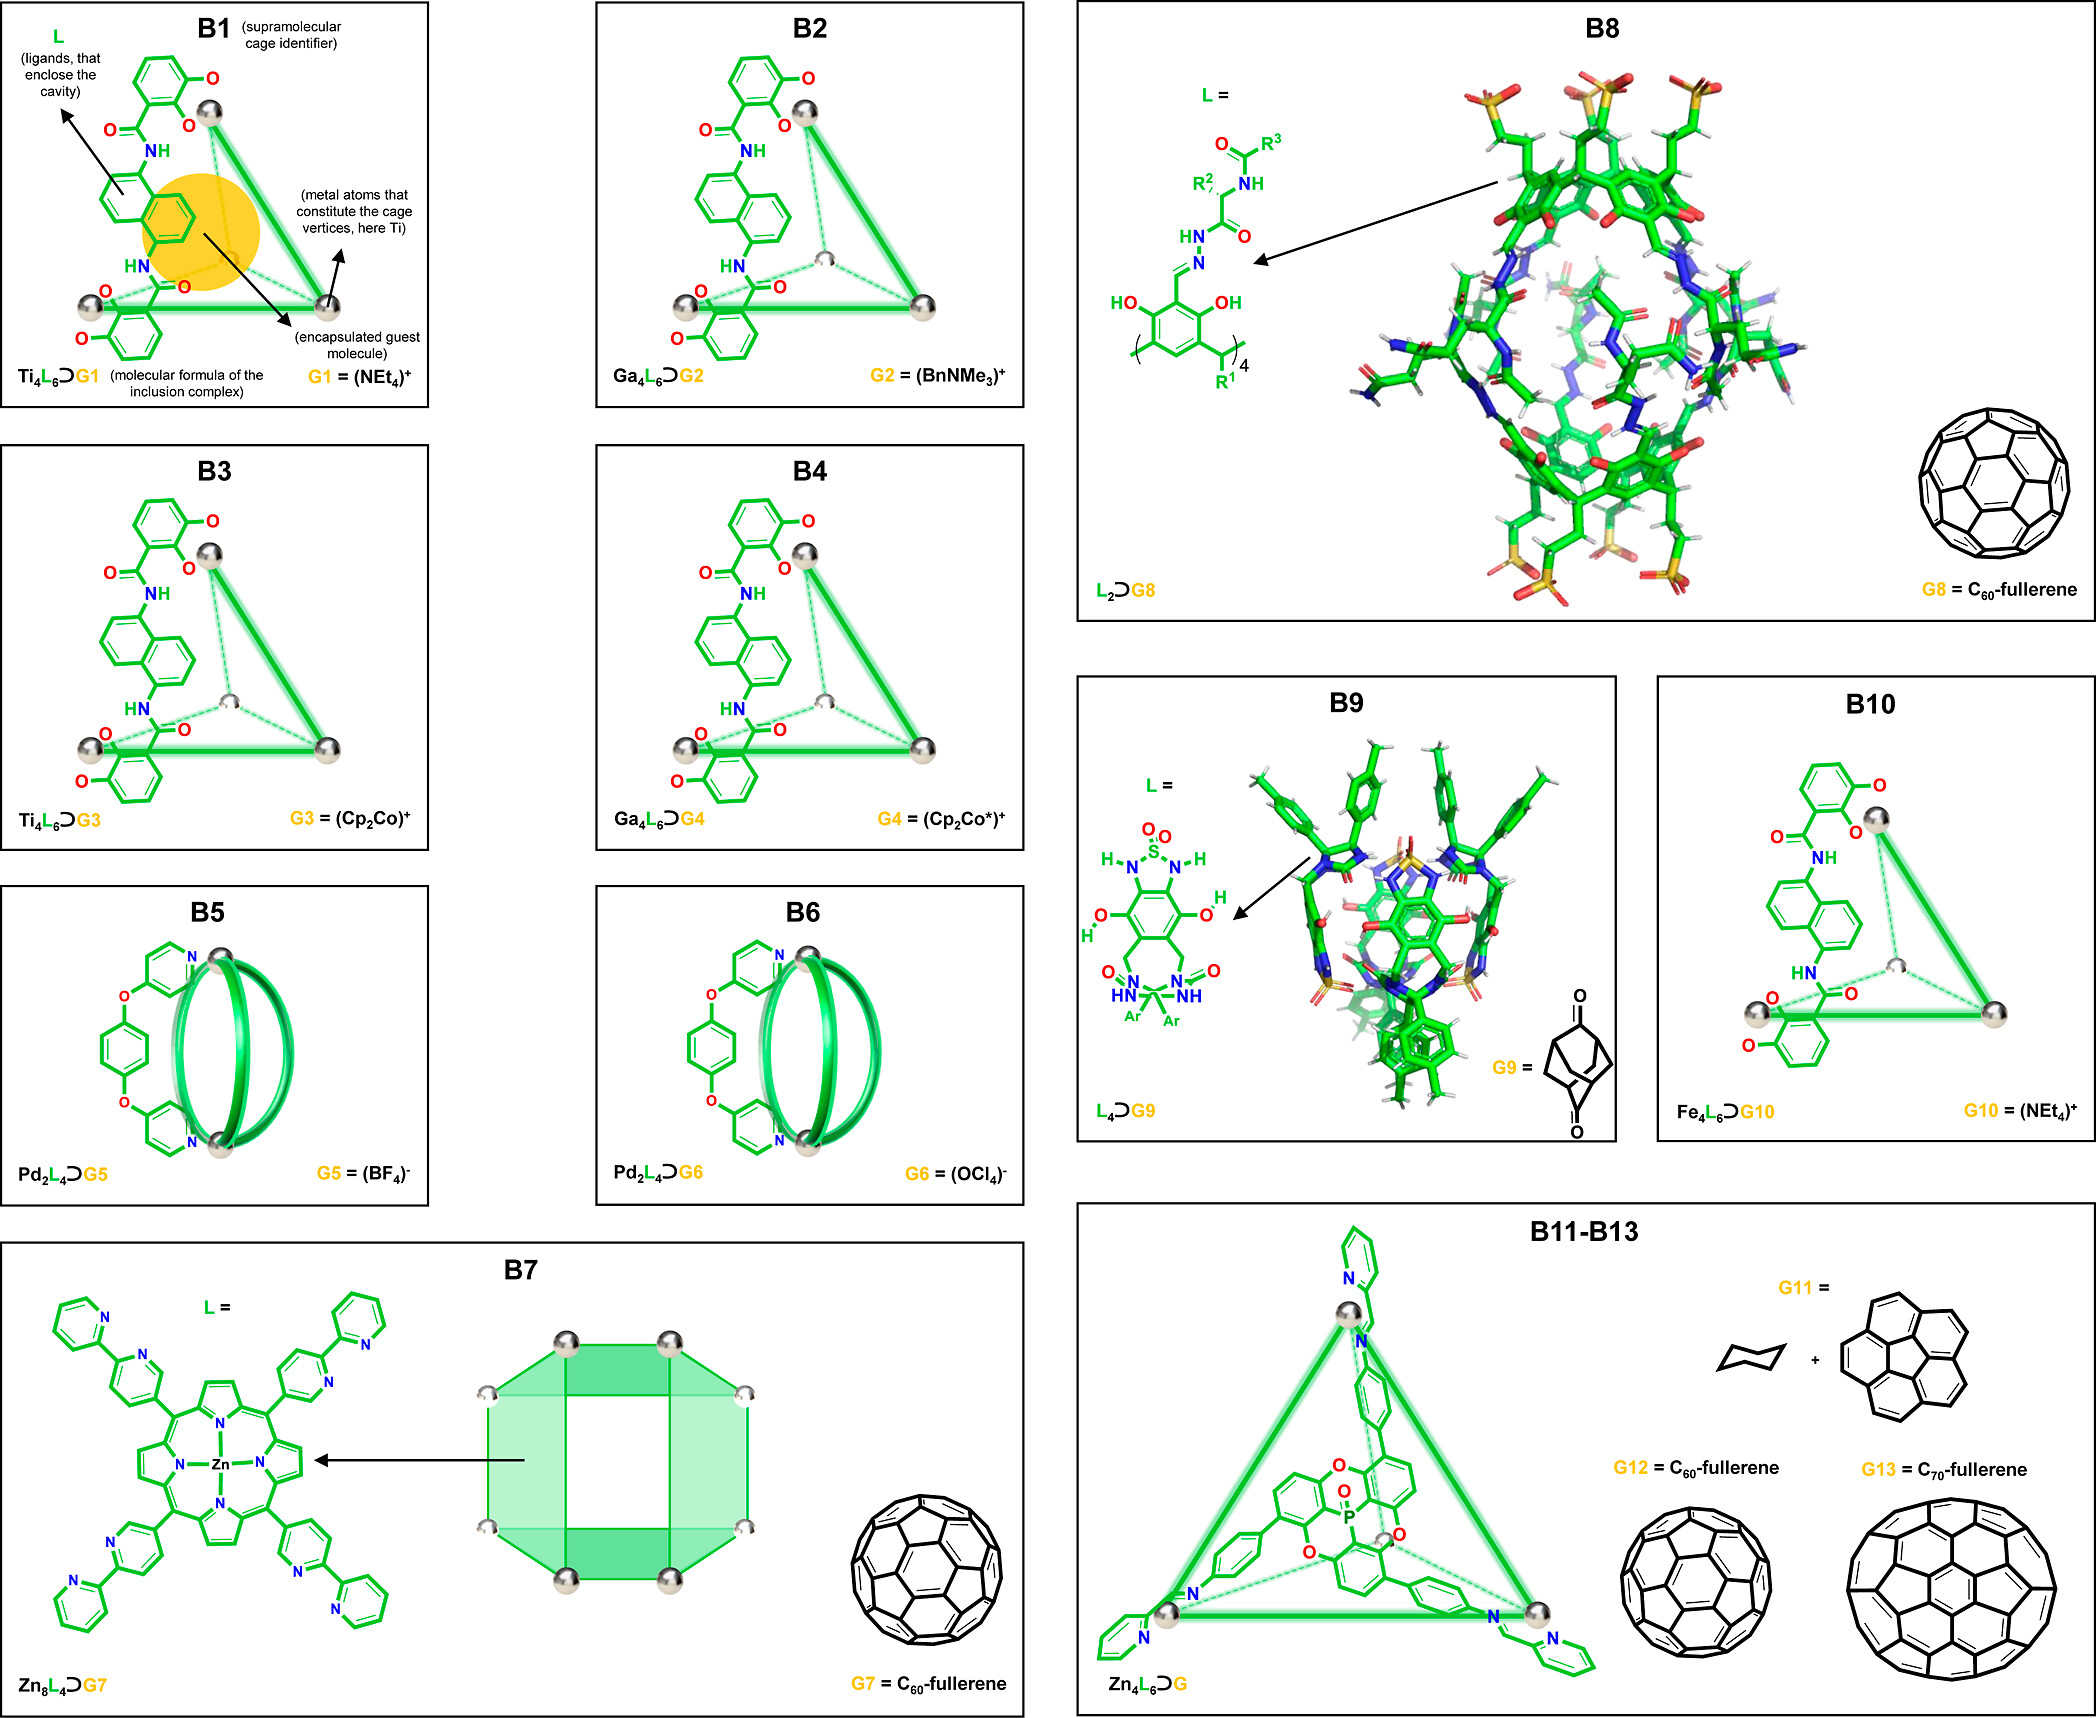
\includegraphics[scale=0.9]{images/benchmark-dataset-1.png}}
  \centerline{\tiny{\textbf{Source:} Reprinted with permission from \cite{guerra2023B}. Copyright 2023 American Chemical Society.}}
  \caption[Benchmark dataset 1]{\textbf{Benchmark dataset 1.} Each of these inclusion complexes features guest molecule(s) ($G_i$) within the cavity of a supramolecular cage ($B_i$). B1: \ch{(NEt4)+} $\subset$ \ch{Ti4L6} (CSD ID: 718468) \cite{pluth2008}. B2: \ch{(BnNMe3)+} $\subset$ \ch{Ga4L6} (CSD ID: 718469) \cite{pluth2008}. B3: \ch{(Cp2Co)+} $\subset$ \ch{Ti4L6} (CSD ID: 718470) \cite{pluth2008}. B4: \ch{(Cp2Co\ast)+} $\subset$ \ch{Ga4L6} (CSD ID: 718471) \cite{pluth2008}. B5: \ch{(BF4)-} $\subset$ \ch{Pd2L4} (CSD ID: 1862753) \cite{steel2018}. B6: \ch{(OCl4)-} $\subset$ \ch{Pd2L4} (CSD ID: 1862752) \cite{steel2018}. B7: \ch{C60} $\subset$ \ch{Zn8L4} (CSD ID: 942782) \cite{nakamura2013}. B8: \ch{C60} $\subset$ \ch{Pd2L4} (CSD ID: 1872778) \cite{eichstaedt2019}. B9: Adamantane-2,6-dione $\subset$ \ch{Pd2L4} (CSD ID: 183906) \cite{johnson2002}. B10: \ch{(NEt4)+} $\subset$ \ch{Pd2L4} (CSD ID: 100947) \cite{caulder1998}. B11: [Corannulene+Cyclohexane] $\subset$ \ch{Pd2L4} (CSD ID: 2068665) \cite{yang2021}. B12: \ch{C60} $\subset$ \ch{Pd2L4} (CSD ID: 2068666) \cite{yang2021}. B13: \ch{C70} $\subset$ \ch{Pd2L4} (CSD ID: 2068667) \cite{yang2021}.}
  \label{fig:benchmark-dataset-1}
\end{figure}

The performance of each cavity detection tool was assessed by comparing the estimated cavity volumes with the "real" cavity volumes (Table \ref{tab:benchmark-1}). 
% TODO: Rewrite this paragraph
% First, to assess this quantitative analysis of the benchmark data set 1, we must analyze the RE values, which consist of the following: (1) error related to the definitions of the cavity boundaries and (2) error related to deviations in the PC from Rebek's rule. To minimize the first error, benchmark data set 1 only contains supramolecular cages with well-defined, closed cavities (void, Figure 10), where the characterization of cavity boundaries is simple and straightforward. On the other hand, deviations from Rebek's rule are more elusive. It has been shown that higher PCs can be reached in inclusion complexes, where in addition to weak dipole-dipole interactions, other forces such as H-bonding, π--π, and CH--π are at work. This results in tighter packing (i.e., PC > 0.55), where the extra stabilization enthalpy counterbalances the loss of entropy (restricted movement of the guest within the cage). Therefore, negative RE is expected in these cases due to the overestimation of cavity volume. For B4--B9, B12, and B13 cages, this trend can be clearly observed in the results of KVFinder project, Fpocket, MoloVol, and CAVER. For B5, B6, and B9, there is experimental evidence for H-bonding interactions. Furthermore, when considering the examples with fullerenes (B7, B8, B12, and B13) and (Cp*)2Co+ (B4) as guests, in addition to weak dipole-dipole interactions, additional π–π and CH-π interactions favor strong host-guest association. For ghecom, pywindow, and POVME, a large negative RE is observed for each supramolecular cage, which suggests that the calculation error of these software becomes more significant. On the other hand, MRAE values clearly show that KVFinder project and Fpocket provide the most reliable cavity volumes.

\begin{table}[H]
  \centering
  \caption[Performance of the well-established cavity detection tools in Benchmark dataset 1]{\textbf{Performance of the well-established cavity detection tools in Benchmark dataset 1.} Estimated cavity volumes by the well-established cavity detection tools. The relative error are calculated using the "real" cavity volume as reference and can be found in paratheses. $V$: "real" cavity volume. $V_{guest}$: guest \acs{vdW} volume. $V = V_{guest} / 0.55$.}
  \scalebox{0.725}{  
    \begin{tabular}{ccccabef}
      \hline
      \textbf{Cage} & \textbf{Guest} & $\boldsymbol{V_{guest}}$ & $\boldsymbol{V}$ & \textbf{KVFinder suite} & \textbf{fpocket} & \textbf{CAVER} & \textbf{GHECOM} \\ \hline
      B1 & \ch{(NEt4)+} & 150 & 273 & 283 (3.7\%) & 247 (-9.5\%) & 396 (44.8\%) & 175 (-35.9\%) \\
      B2 & \ch{(BnNMe3)+} & 155 & 281 & 283 (0.8\%) & 279 (-0.6\%) & 339 (20.8\%) & 192 (-31.7\%) \\ 
      B3 & \ch{(Cp2Co)+} & 137 & 248 & 269 (8.1\%) & 277 (11.6\%) & 335 (34.9\%) & 191 (-23.3\%) \\
      B4 & \ch{(Cp2Co\ast)+} & 309 & 562 & 438 (-22.1\%) & 434 (-22.7\%) & 474 (-15.7\%) & 343 (-39.0\%) \\ 
      B5 & \ch{(BF4)-} & 50 & 90 & 78 (-13.6\%) & 84 (-6.5\%) & 65 (-27.5\%) & 29 (-67.6\%) \\ 
      B6 & \ch{(OCl4)-} & 53 & 96 & 81 (-15.6\%) & 82 (-14.3\%) & 79 (-17.4\%) & 64 (-33.7\%) \\ 
      B7 & \ch{C60} & 519 & 944 & 757 (-19.8\%) & 771 (-18.3\%) & 778 (-17.6\%) & 734 (-22.3\%) \\ 
      B8 & \ch{C60} & 512 & 930 & 731 (-21.4\%) & 805 (-13.5\%) & 682 (-26.7\%) & 704 (-24.3\%) \\ 
      B9 & Adamantane-2,6-dione & 141 & 257 & 155 (-39.5\%) & 181 (-29.5\%) & 173 (-32.5\%) & 159 (-38.0\%) \\ 
      B10 & \ch{(NEt4)+} & 151 & 274 & 251 (-8.4\%) & 225 (-17.7\%) & 351 (28.1\%) & 161 (-41.1\%) \\ 
      B11 & [Corannulene+Cyclohexane] & 307 & 558 & 496 (-11.0\%) & 482 (-13.6\%) & 457 (-18.1\%) & 401 (-28.1\%) \\ 
      B12 & \ch{C60} & 524 & 954 & 737 (-22.7\%) & 627 (-34.2\%) & 742 (-22.2\%) & 606 (-36.5\%) \\ 
      B13 & \ch{C70} & 618 & 1123 & 872 (-22.3\%) & 811 (-27.7\%) & 1031 (-8.1\%) & 752 (-33.0\%) \\ \hline
      \textbf{MRAE} &  &  &  & \textbf{16.1\%} & \textbf{16.9\%} & \textbf{24.2\%} & \textbf{35.0\%} \\ \hline
    \end{tabular}
  }
  \label{tab:benchmark-1}
\end{table}

% TODO: Rewrite this paragraph
% A visual representation of the software performance (Figure 12A) shows that volumes calculated with KVFinder project and Fpocket are close to the estimated volume with a small spread compared to other software. Despite a few outlying results, the overall trend (vide supra) supports our approach of using Rebek's rule as the best estimate for the “real” cavity volume within these supramolecular cages.

\subsection{Benchmarking Dataset 2}

% TODO: Rewrite this paragraph
% The benchmark dataset 2 (Figure \ref{fig:benchmark-dataset-2}) comprises 9 X-ray structures of well-known supramolecular cages, without the guest molecules, but with different topological and morphological features (\ie, cavity size, opening size, and shape). This dataset aims to evaluate the capabilities and limitations of the well-established cavity detection tools in detecting different types of cavities (Figure \ref{fig:cavity-classification}). However, these supramolecular cages do not contain guests inside their cavity, so the "real" cavity volume estimation cannot be calculated by the Rebek's rule of thumb. Consequently, the average volume of detected cavities was chosen as the point of comparison to calculated volumes (Table \ref{tab:benchmark-2}), which establishes an agreement between methods by mitigating deviations in volume data.

\begin{figure}
  \centerline{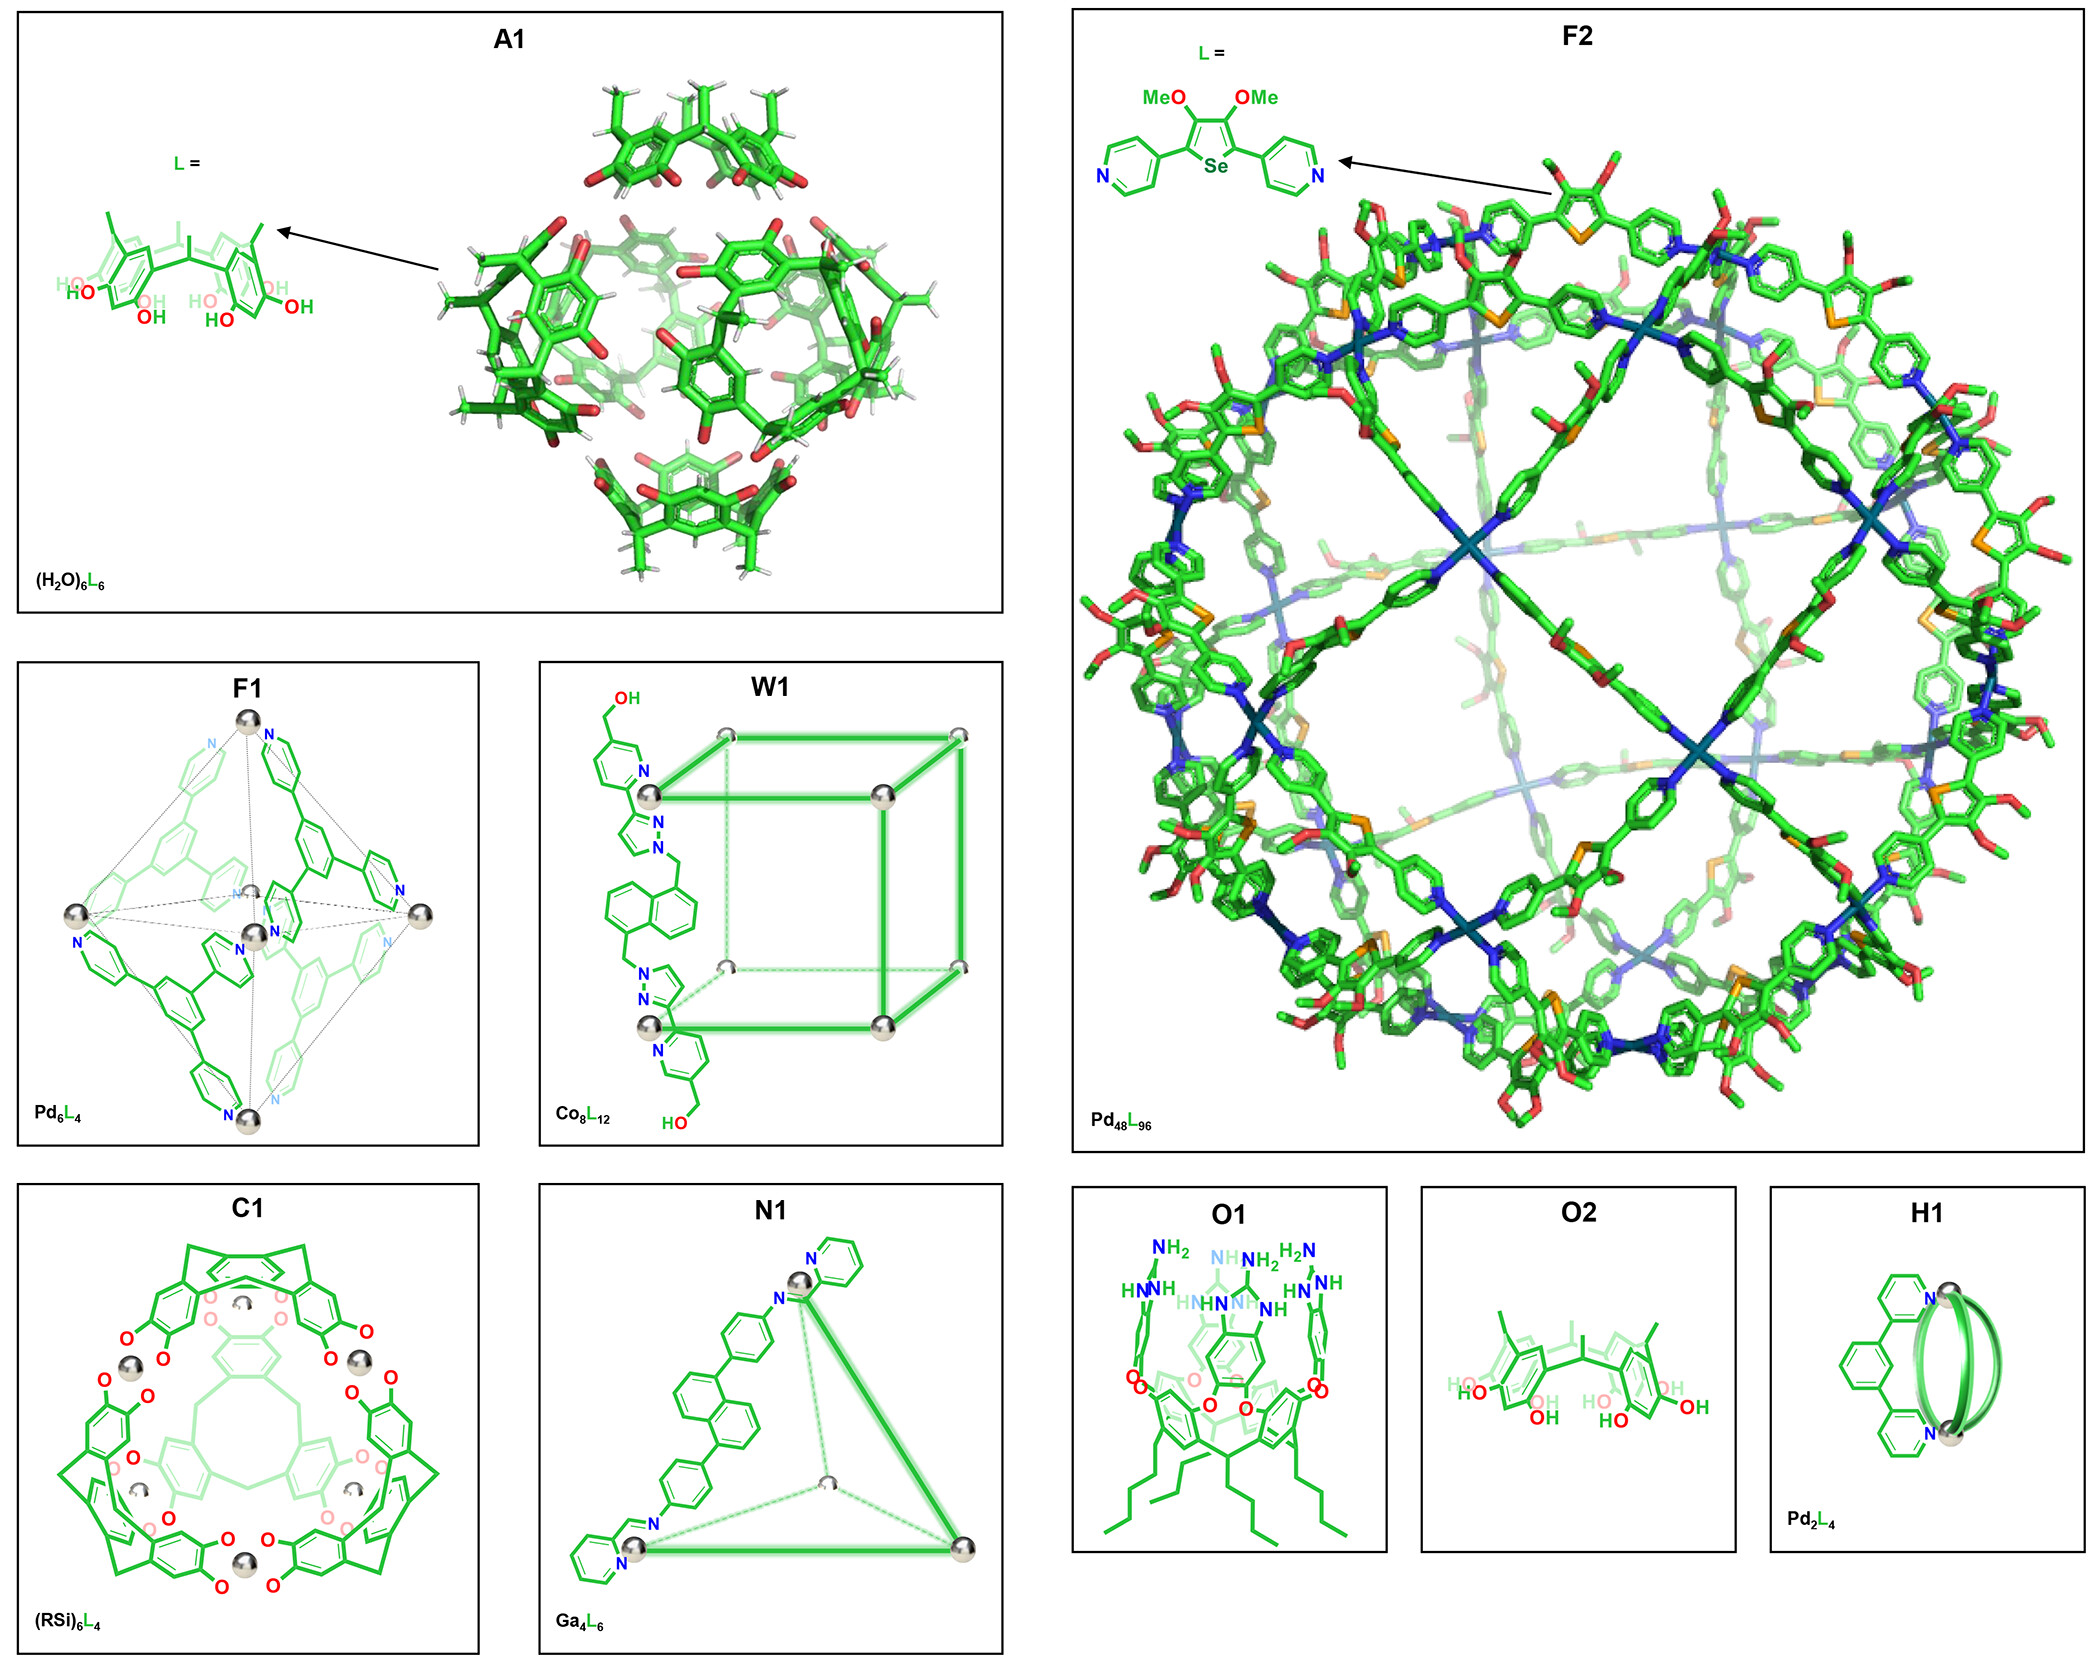
\includegraphics[scale=0.9]{images/benchmark-dataset-2.png}}
  \centerline{\tiny{\textbf{Source:} Reprinted with permission from \cite{guerra2023B}. Copyright 2023 American Chemical Society.}}
  \caption[Benchmark dataset 2]{\textbf{Benchmark dataset 2.}
  A1: \ch{(H2O)6L6} (CSD ID: 1207879) \cite{macgillivray1997}.
  C1: \ch{(RSi)6L4} (CSD ID: 1892128) \cite{kawakami2019}.
  F1: \ch{Pd6L4} (CSD ID: 293777) \cite{yoshizawa2006}.
  F2: \ch{Pd48L96} (CSD ID: 1831430) \cite{fujita2016}.
  H1: \ch{Pd2L4} (CSD ID: 768969) \cite{liao2010}.
  N1: \ch{Ga4L6} (CSD ID: 1541839) \cite{ronson2017}.
  O1: Cavitand bearing 2-Aminobenzimidazole walls and pyridinium feet (CSD ID: 2074472) \cite{zhang2021}.
  O2: Resorcin[4]arene (CSD ID: 1207879) \cite{macgillivray1997}.
  W1: \ch{Co8L12} (CSD ID: 1416694) \cite{cullen2016}.}
  \label{fig:benchmark-dataset-2}
\end{figure}

It is important to note that the cavity detection benchmarking procedure, optimized detection parameters, and detailed results are available in the article published in the \textit{Journal of Chemical Information and Modeling} \cite{guerra2023B}. 

\subsection{Discussion}

% TODO: Rewrite this paragraph
% In summary, each software has its own capabilities and shortcomings that derive from the type of cavity detection method applied, its implementation, and its software interfaces (Table 3). In general, grid-and-sphere-based and tessellation-based methods give the most precise cavity volumes, while grid-based and sphere-based methods performed worse. As previously described, pywindow uses an algorithm that defines the cavity volume as the volume of the largest sphere that can be fitted within the cavity. Therefore, pywindow consistently underestimates the cavity size of nonspherical cavities (F1, H1, N1, W1, and O1) and shallow grooves (O2). Grid-, sphere-, and grid-and-sphere-based methods can detect any type of cavities in supramolecular cages, except for ghecom and CAVER Analyst 2.0, which, together with tessellation-based methods, fail to detect clefts and grooves. Taking into account our assessment, KVFinder project and Fpocket overperformed the other software in benchmarking as they provide volumes closest to the estimated and average volumes, with a small spread compared to other software (Figure 12A and 12B).

% All these methods are accessible to users with a simple and well-documented installation, configuration, and execution. From this perspective, the software interfaces available to users, i.e., graphical user interface (GUI), command line interface (CLI), application programming interface (API), and web application, dictate the pool of viable applications for each software. Commonly, GUIs and Web Applications are simpler and easier for less-experienced users to execute due to visual aids that intuitively guide the user through the analysis pipeline. However, these interfaces lack efficiency when performing analysis with large data sets, e.g., high-throughput analysis (HTA), MD simulations, machine learning (ML), deep learning (DL), virtual screening (VS) applications, and automating pipelines. In this sense, CLIs and APIs are efficient and integrable software interfaces, which allow the development of applications with large data sets and pipeline automation; however, they are highly dependent on their documentation to the user interaction with the software efficiently. Also, the main drawback of CLI is that it provides black-box applications, which do not allow users to fully customize pipeline automation since some variables are not definable by the user. On the other hand, APIs (e.g., pyKVFinder, pywindow, and fpocket) are the most versatile interfaces, where users can use them as building blocks for more complex applications and/or integrate them with third-party scientific packages, e.g., numpy, scipy, scikit-learn, and matplotlib. Additionally, pyKVFinder has its core data structures accessible and easy-to-handle, allowing the development of new characterizations and applications built around them.

\section{Perspectives}

% Data science
% DL/ML applications
% Druggability/Ligandability
% Virtual Screening
% New characterizations such as skeletonize cavities (measure of accessibility)

%%% Chapter 6

\chapter{Conclusion}

% Após estudo cuidadoso das demandas de ferramentas computacionais da comunidade de biologia estrutural, desenvolvemos com sucesso a plataforma computacional KVFinder suite. Essa plataforma foi projetada para estudos de sistemas biomoleculares, fornecendo ferramentas abrangentes de codificação e caracterização de biomoléculas e seus sítios de ligação. O KVFinder suite é composto por 5 ferramentas computacionais, englobando diferentes demandas e objetivos da comunidade de biologia estrutural, que são o KVFinder-web, parKVFinder, pyKVFinder, SERD e KVFinderMD. 

% O KVFinder-web é uma aplicação web de código aberto para detecção e caracterização de cavidades, usando o parKVFinder, em qualquer tipo de estrutura biomolecular. O KVFinder-web visa ampliar o uso do parKVFinder na comunidade científica, além de democratizar o acesso e remover barreiras para usuários que não possuem conhecimento técnico para instalar e configurar uma ferramenta computacional, que possuem recursos computacionais limitados ou que desejam realizar uma análise simples e rápida. A aplicação web está disponível em \url{https://kvfinder-web.cnpem.br}.

% O parKVFinder é uma ferramenta de código aberto desenvolvida para a detecção e caracterização de cavidades biomoleculares. Ele inclui um plugin gráfico integrado ao visualizador molecular PyMOL, que oferece uma interface intuitiva para explorar parâmetros personalizáveis e visualizar as cavidades detectadas e suas características. Embora o parKVFinder tenha limitações em aplicações automatizadas e comparações sistemáticas de sítios de ligação, ele desempenha um papel importante na otimização dos parâmetros de detecção e caracterização por meio do plugin gráfico do PyMOL (PyMOL2 parKVFinder Tools), devido aos seus recursos visuais. Estes parâmetros otimizados podem ser posteriormente adotados em estudos automatizados e comparações sistemáticas de sítios de ligação.

% O pyKVFinder é um pacote Python de código aberto para detectar e caracterizar cavidades em estruturas biomoleculares em protocolos automatizados e aplicações de ciência de dados. Além de possuir as mesmas funcionalidades do KVFinder-web e parKVFinder, o pyKVFinder fornece estruturas de dados acessíveis e flexíveis no ecossistema Python, como \textit{ndarrays} e dicionários. Isso permite que os usuários desenvolvam novas caracterizações de cavidades e protocolos de análise baseados nessas estruturas de dados, facilitando a exploração eficiente e eficaz das cavidades biomoleculares e impulsionando a descoberta de novos alvos terapêuticos e o desenvolvimento de medicamentos mais eficazes.

% Dentro do contexto do pyKVFinder, em colaboração com o Dr. György Szalóki, expandimos a metodologia de detecção e caracterização de cavidades para uma nova classe de moléculas chamadas de gaiolas supramoleculares. Além disso, desenvolvemos novas caracterizações aplicáveis tanto à gaiolas quanto à biomoléculas, incluindo a modelagem da superfície molecular em grades 3D, a estimativa de volume molecular e a caracterização de aberturas das cavidades. Essas implementações podem servir como guia para os usuários desenvolverem novas caracterizações.

% Ao longo do projeto, avaliamos continuamente o desempenho computacional e a capacidade de detecção de cavidades das ferramentas do KVFinder suite (\eg, KVFinder-web, parKVFinder e pyKVFinder), comparando-as com outras metodologias disponíveis. Os resultados atestaram a eficácia e o desempenho computacional dessas ferramentas. No entanto, estas ferramentas citadas acima dependem da modelagem e descrição em grades 3D. Para abranger uma gama mais ampla de codificações de biomoléculas e sítios de ligação, desenvolvemos a ferramenta SERD. Essa ferramenta expandiu as possibilidades de codificação na plataforma KVFinder suite, incluindo a representação topológica dos resíduos de interface e a representação em forma de grafos. Essa flexibilidade permite a aplicação de diferentes codificações em estudos de sistemas biomoleculares.

% Por fim, desenvolvemos o KVFinderMD, um pacote em Python que permite explorar a dinâmica dos sítios de ligação em estruturas biomoleculares de interesse farmacológico. Essa ferramenta exemplifica a capacidade do pyKVFinder de fornecer protocolos automatizados para análises sistemáticas de sítios de ligação. A análise da similaridade das cavidades da protease do HIV-1 ao longo de uma simulação de DM permitiu acompanhar a evolução das cavidades e comparar suas características ao longo do tempo. Utilizando algoritmos de agrupamento hierárquico e diferentes métricas de afinidade em diferentes codificações (\ie, representações em grade 3D, representação topológica e representação em grafo), identificamos grupos de cavidades mais similares. Além disso, pudemos reduzir o tamanho dos dados necessários à análise de similaridade e simplificar da comparação entre as cavidades em simulações de DM, demonstrando a aplicabilidade prática do KVFinder suite.

% Em resumo, a plataforma computacional KVFinder suite simplifica o estudo de sistemas biomoleculares de interesse terapêutico, incluindo a caracterização de biomoléculas e seus sítios de ligação, mesmo para usuários menos experientes. Isso tem um impacto direto na busca e no desenho racional de fármacos, assim como na compreensão das estruturas de biomoléculas.

% As referências:
\bibliographystyle{abnt-num}
\bibliography{phdthesis}

% Os anexos, se houver, vêm depois das referências:
\appendix

% \section{KVFinderMD}

% \subsection{Estudo comparativo dos sítios de ligação do substrato da ALDH1 e ALDH2}

% o caso das ALDH1/2, exploramos as diferenças topológicas e volumétricas entre os sítios de ligação do substrato de ALDH1 e ALDH2, o que dita a preferência por aldeídos menores e maiores entre eles.

\end{document}
